The search for supersymmetric particles is among the most important goals of the LHC physics program. As discussed in Sec.~\ref{subsec:susy_collider}, searches performed at $\sqrt{s} = 7$\tev have constrained the allowed parameter space for light-flavour squarks and gluinos already up to around 800\gev and 1\tev for light LSP masses, respectively. However, the increased centre of mass energy from 7\tev to 8\tev and the recorded dataset, which is around four times larger than at 7\tev, provide the opportunity to extend the reach of such searches into entirely unexplored parameter regions. In Fig.~\ref{fig:susy_theory_xs}, the theory cross section for the production of supersymmetric particles is shown as a function of the SUSY particle mass. The $y$-axis on the right indicates how many events are expected in 20\fbinv of \pp collision data at the LHC at $\sqrt{s}=8$\tev. 
\begin{figure}[!h]
  \centering
  \begin{tabular}{c}
                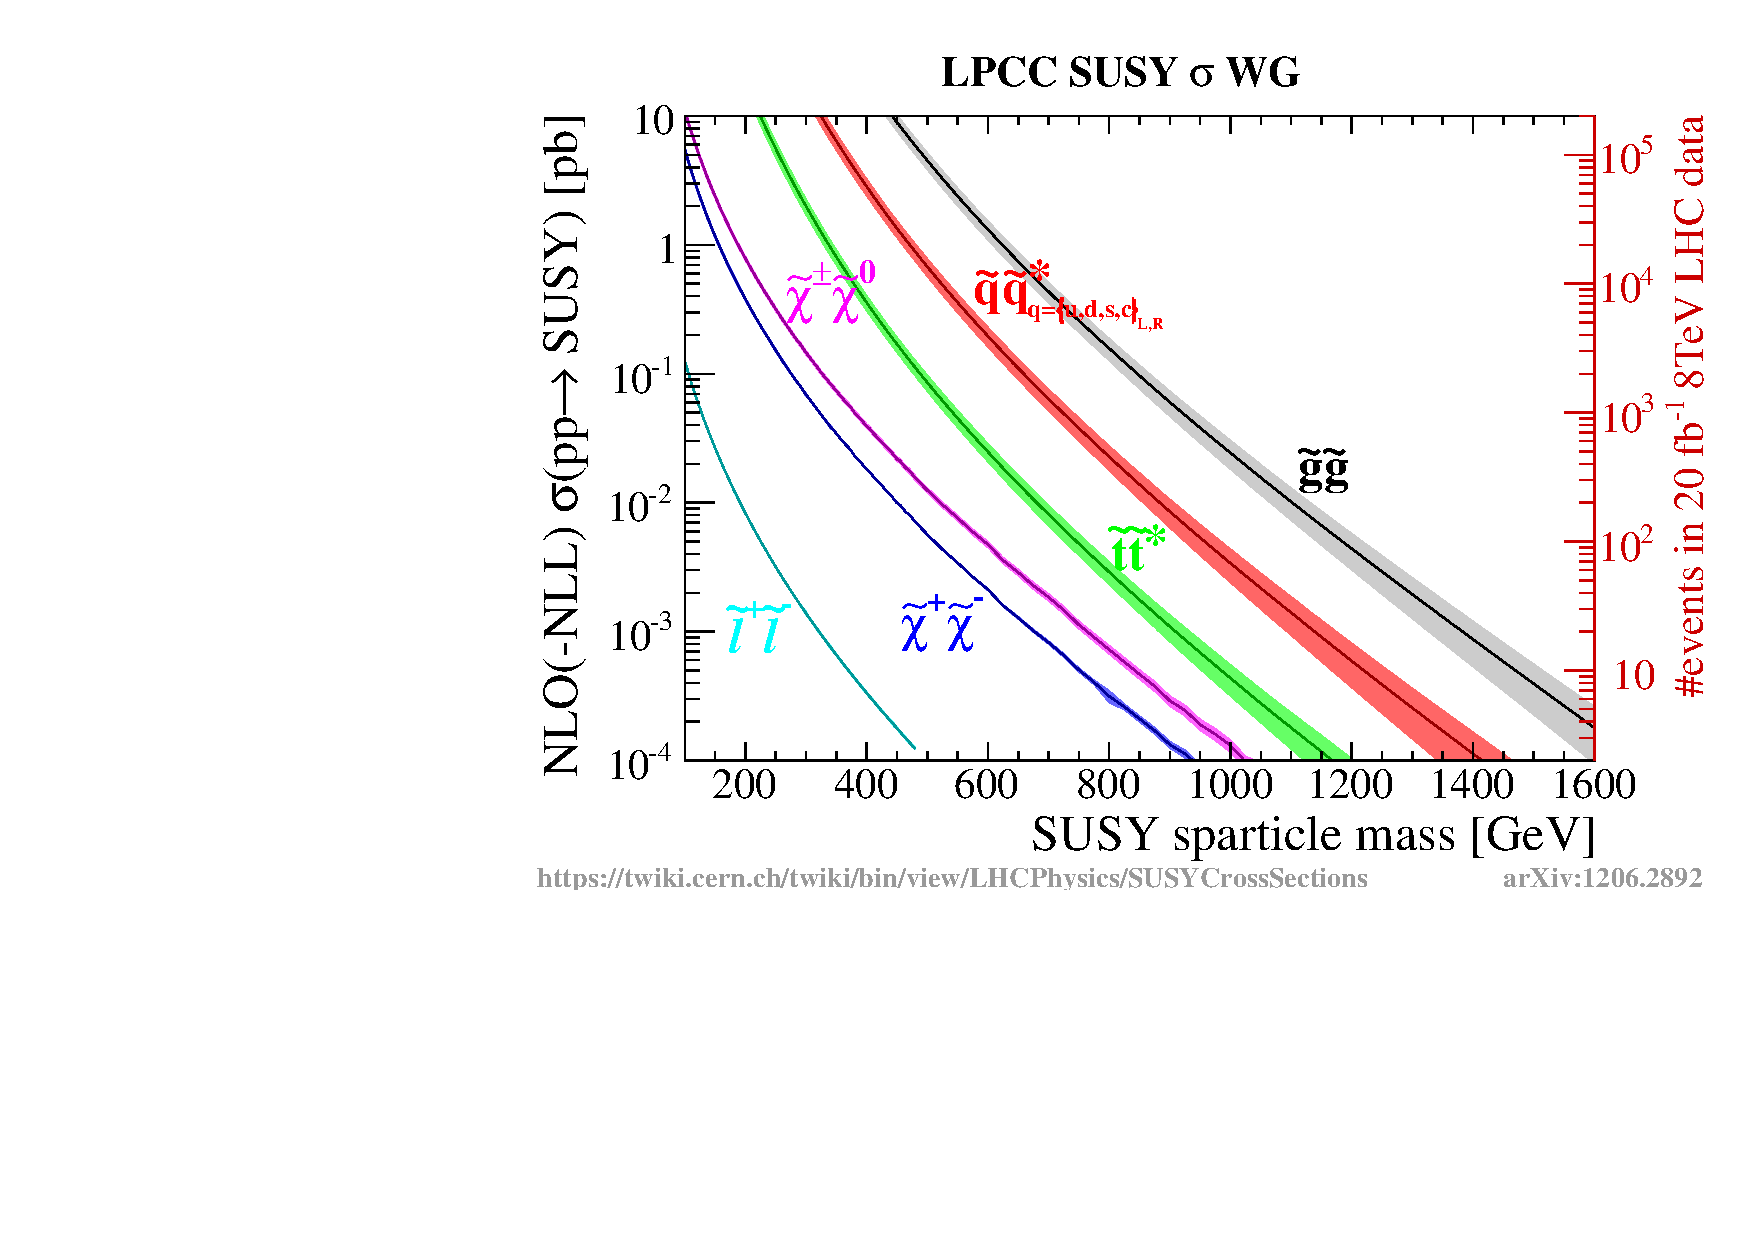
\includegraphics[width=0.65\textwidth]{figures/xsections_strong.pdf} 
  \end{tabular}
  \caption{Theory cross sections for selected SUSY processes as a function of the sparticle mass. The $y$-axis on the right indicates the expected number of events in 20\fbinv of \pp collision data at the LHC at $\sqrt{s}=8$\tev~\cite{Kramer:2012bx}.}
  \label{fig:susy_theory_xs}
\end{figure}
\\
Especially light-squarks and gluinos are expected at a sizable rate, even for high masses above 1\tev. For instance, around 100 pairs of gluinos are expected at a mass of 1200\gev. \\
The analysis presented in this chapter searches for supersymmetric cascade decays arising from strongly produced light-flavour squarks or gluinos. As introduced in Sec.~\ref{subsec:susy_collider}, the expected experimental signature contains several hard jets and a certain amount of missing transverse energy. Thus, events are selected based on the number of jets (\NJets), the scalar sum of the jet transverse momenta (\HT) and the missing transverse momentum calculated from the jet momenta (\MHT). However, the generic structure makes the analysis in principle sensitive to any new physics model that manifests in final states containing several hard jets accompanied by missing transverse energy, in case the cross section of the process and the acceptance of the selection is large enough. \\
After the description of the event selection (Sec.~\ref{sec:RA2_sel}), it is discussed how contributions from standard model processes to the selected final state are estimated. Special emphasis is put on the estimation of the QCD multijet background (Sec.~\ref{subsec:RA2_QCD}). Finally, results are presented and interpreted in various simplified supersymmetric models (Sec.~\ref{sec:RA2_results}). Parts of this chapter are taken from~\cite{bib:AN-12-350}, written by the author. This analysis follows previous inclusive searches~\cite{springerlink:10.1007/JHEP08(2011)155, Chatrchyan:2012lia} and is published in~\cite{Chatrchyan:2014lfa}.
    
\section{Event Selection}
\label{sec:RA2_sel}
\subsection{Data Samples}
\label{subsec:RA2_samples_trigger}
The analysis is based on \pp collision data recorded with the CMS detector at a centre of mass energy of $\sqrt{s} = 8$\tev. This corresponds to an integrated luminosity of 19.5\fbinv for all sub-detectors fully functional. \\
In addition, it is made use of several simulated samples describing SM background processes. These are especially employed in the validation of the background estimation methods described in Sec.~\ref{sec:RA2_Non-QCD} and~\ref{subsec:RA2_QCD}. The standard model processes for \ttbar, \WJets, \ZJets, $\gamma + \mathrm{{jets}}$ and QCD multijet events are generated with the \madgraph~\cite{Alwall:2014hca} generator at leading order and are interfaced with the parton-shower model in \pythia 6.4.24~\cite{Sjostrand:2006za}. While \ttbar events are generated with up to three additional jets, other background samples contain up to four additional jets. The samples are scaled to cross-section predictions at next-to-leading order or next-to-next-to-leading order, when available~\cite{Kidonakis:2010dk, Melnikov:2006kv}. The events are processed with the full detector simulation. 
%\begin{table}[!t]
%\fontsize{9 pt}{1.2 em}
%\selectfont
%\centering
%\caption{Overview of simulated background samples used in the analysis and corresponding production cross sections.}
%\makebox[\linewidth]{
%\begin{tabular}{llrc}
%\multicolumn{4}{c}{} \\
%\toprule
%   Process &  & $\sigma$ [pb] & Precision \\
%   \midrule
%   \midrule
%   \ttbar & semi-leptonic decays & 102.5 & NNLO \\
%          & fully-leptonic decays & 24.6 & NNLO \\
%          & hadronic decays & 106.9 & NNLO \\
%   \midrule
%   \WJets & \HT = [400, $\infty$]\gev  & 30.1 & NNLO \\
%   \midrule
%   \ZJets & \HT = [400, $\infty$]\gev & 6.3 & NNLO \\
%   \midrule
%   QCD multijet & \HT = [100, 250]\gev & $1.04 \cdot 10^7$& LO \\
%                & \HT = [250, 500]\gev & $276\,000.0$ & LO \\
%                & \HT = [500, 1000]\gev & 8426.0 & LO \\
%                & \HT = [1000, $\infty$]\gev & 204.0 & LO \\
%   \bottomrule
%\end{tabular}}
%\label{tab:ra2_samples}
%\end{table}    
\\
Furthermore, SUSY signal samples are obtained from simulation. They are generated with \madgraph~\cite{Alwall:2014hca} (with up to two additional partons), the CTEQ6L parton distribution functions~\cite{Pumplin:2002vw} and processed with the fast detector simulation. Cross sections are determined at NLO with a resummation of soft gluon emission at the accuracy of next-to-leading-log~\cite{Beenakker:1996ch, PhysRevLett.102.111802, PhysRevD.80.095004, Beenakker:2009ha, Beenakker:2011fu, Kramer:2012bx}. The cross section calculation as well as the generation of signal events for a certain type of sparticle is performed by effectively removing contributions from other sparticles by assuming their mass to be very large.

\subsection{Trigger}
\label{subsec:RA2_trigger}
\begin{table}[!t]
\centering
\caption{Signal trigger paths used in different run ranges listed together with the integrated luminosity.}
\label{tab:RA2_trigger}
 \makebox[\linewidth]{
\begin{tabular}{lccc}
\multicolumn{4}{c}{} \\
\toprule
 Trigger path & Run range & Luminosity [\fbinv] \\
\midrule
 HLT\_PFHT350\_PFMET100 & 190456--196531 & 0.9 \\
 & & & \\
 HLT\_PFHT350\_PFMET100 & 190782--190949 & 4.4 \\
 & & & \\
 HLT\_PFNoPUHT350\_PFMET100 & 198022--198523 & 6.9 \\
 & & & \\
 HLT\_PFNoPUHT350\_PFMET100 & 198524--208686 & 7.3 \\
\bottomrule
\end{tabular}}
\end{table}  
The data have been collected by triggering on \HT, the scalar sum of the jet transverse momenta, and \met, the missing transverse energy. An overview of the considered runs and the integrated luminosity is shown together with the respective HLT trigger paths in Tab.~\ref{tab:RA2_trigger}. \HT and \met are calculated from particle-flow objects at trigger level with nominal thresholds of 350\gev and 100\gev, respectively. Jets considered in this calculation are reconstructed with the anti-$k_T$ algorithm and distance parameter $R = 0.5$. The labelling \textit{PFNoPU} indicates that, for that particular runs, also charged-hadron subtraction was applied to jets at trigger level. \\
In order to determine the offline values for \HT and \MHT (calculated according to the definition following in Sec.~\ref{subsec:RA2_baseline}) for which the triggers reach the plateau efficiency, the trigger efficiencies are measured with respect to a single electron trigger (HLT\_Ele27\_WP80), \ie it is tested how many events that are triggered by the reference electron trigger also pass the trigger under study. In principle, an independent trigger is desirable in order to get an unbiased estimate of the trigger efficiency. However, due to the PF-algorithm all subdetectors are used simultaneously to reconstruct the particles in an event. Hence, no independent trigger paths providing enough statistical precision are available. Consequently, only the reach and position of a plateau efficiency for a certain trigger path can be determined. \\
The determination of the relative trigger plateau efficiency is performed for different jet multiplicity intervals ($3 \leq \NJets \leq 5$, $6 \leq \NJets \leq 7$ and \NJets~$ \ge 8$). The obtained trigger turn-on curves for the two different HLT paths are shown as a function of \HT and \MHT, as used in the analysis, for jet multiplicity $3 \leq \NJets \leq 5$ in Fig.~\ref{fig:trig_eff_3njets5}. The respective turn-on curves for jet multiplicities $6 \leq$ \NJets $\leq 7$ and \NJets~$ \ge 8$ are shown in App.~\ref{fig:trig_eff_6njets7} and App.~\ref{fig:trig_eff_njets8}. For both trigger paths, the efficiency plateau is reached around values of \HT$ = 500$\gev and \MHT$ = 200$\gev. \\
The integrated trigger efficiencies for these particular values in different jet multiplicity intervals are summarized with statistical uncertainties in Tab.~\ref{tab:trig_eff}. In general, they are close to 100\% with small uncertainties below 1\%. However, for the highest jet multiplicity selection of \NJets~$ \ge 8$ only few events where selected such that statistical uncertainties are few 10\% large. Though, no hints for a systematic inefficiency have been observed and the signal triggers are considered as fully efficient with an uncertainty of $2\%$ for values of \HT$ > 500$\gev and \MHT$ > 200$\gev independent of the jet multiplicity. 
\begin{figure}[!t]
  \centering
  \begin{tabular}{cc}
                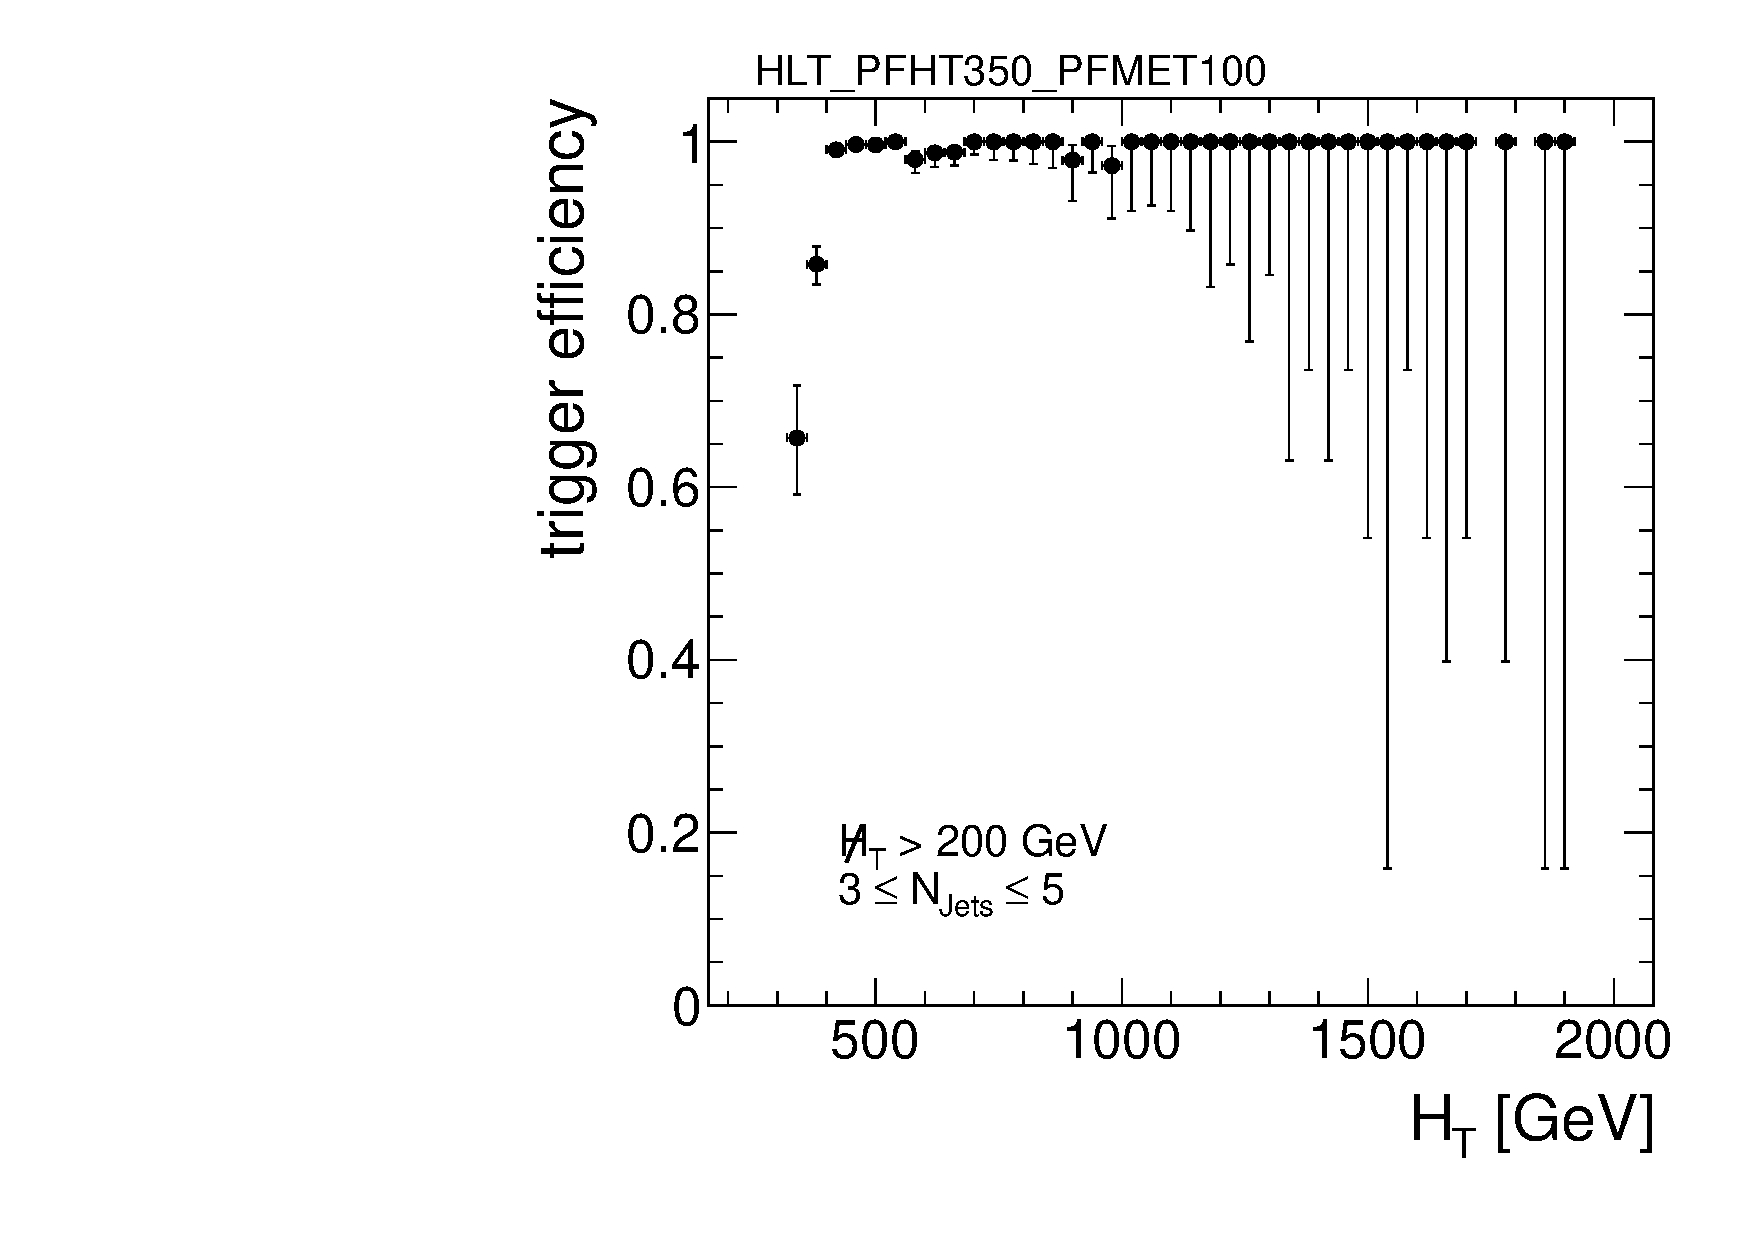
\includegraphics[width=0.47\textwidth]{figures/turn_on_HT_TagEle27WP80_ProbePFHT350PFMET100_MHT200_chs_NJets3-5.pdf} &
                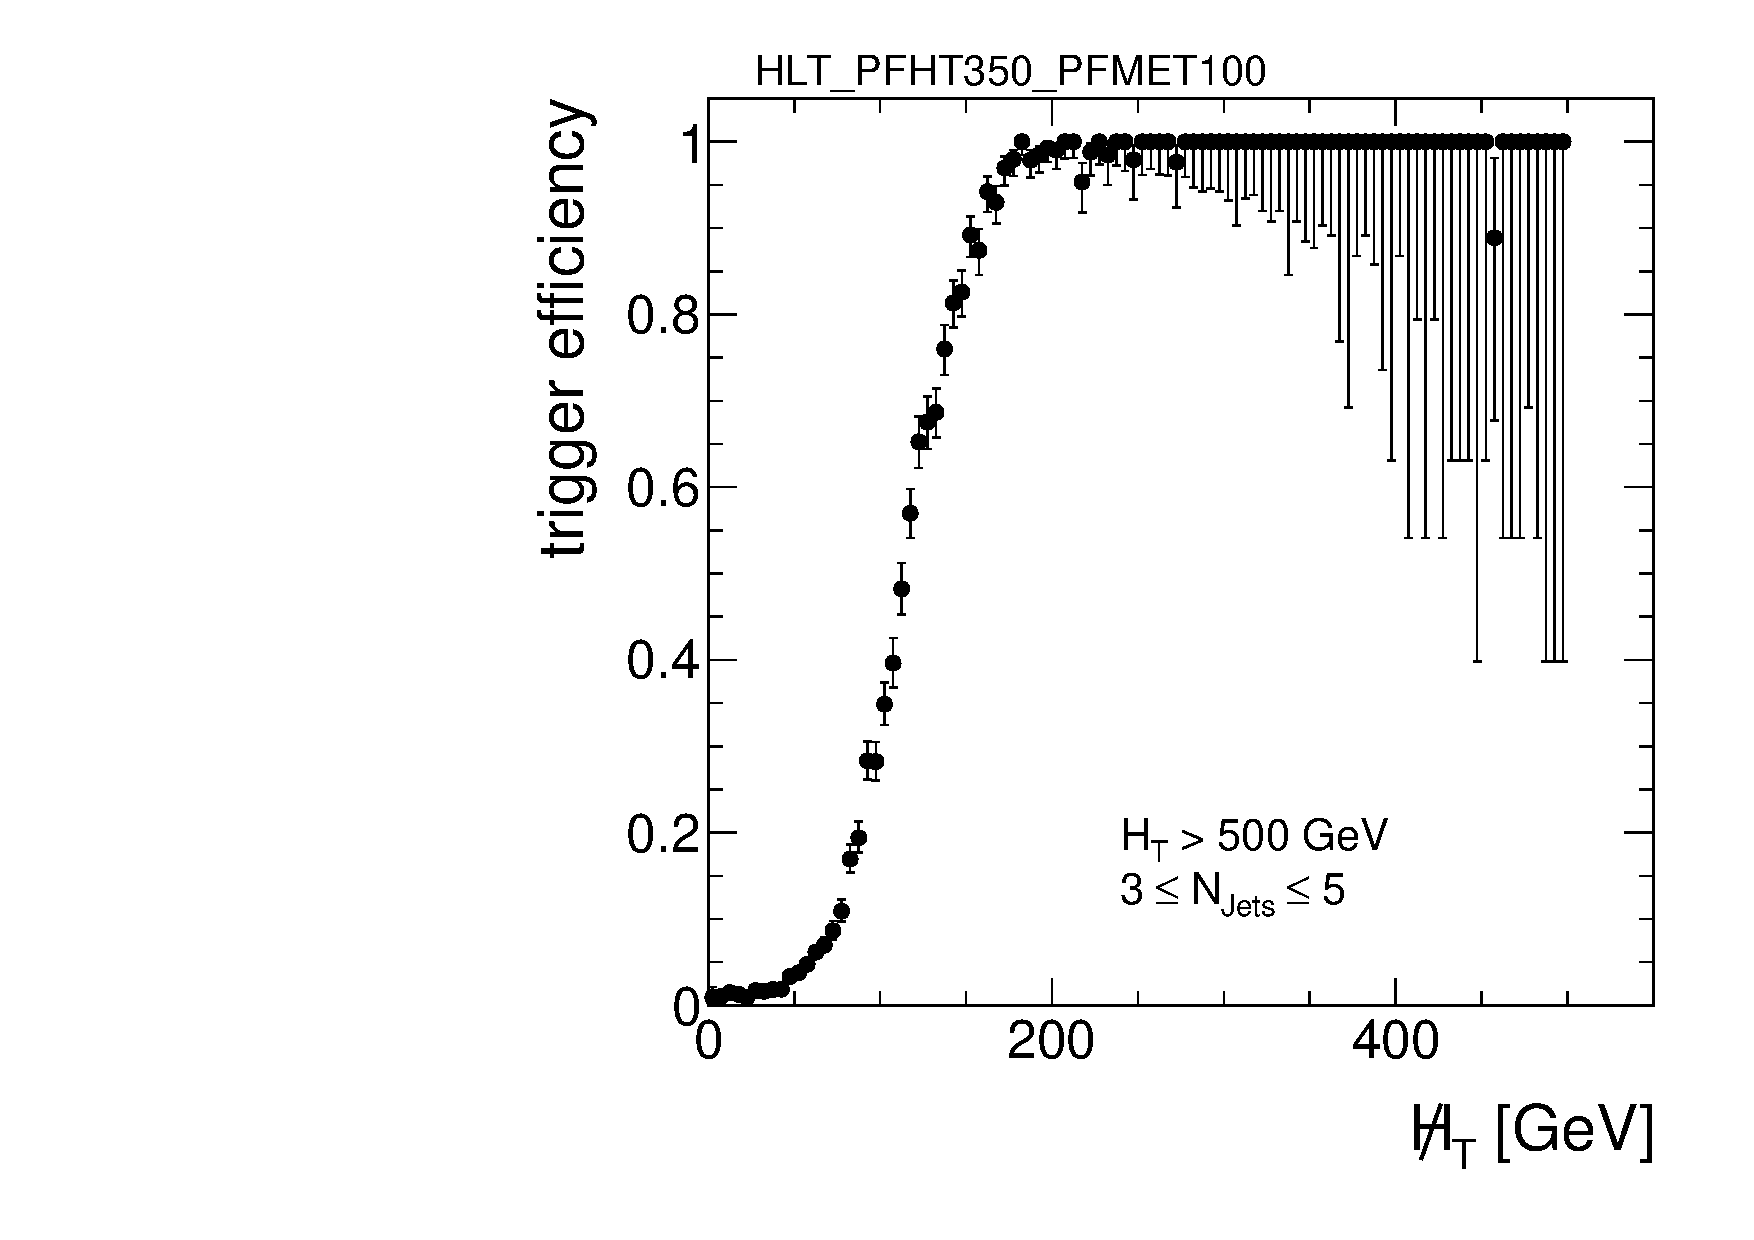
\includegraphics[width=0.47\textwidth]{figures/turn_on_MHT_TagEle27WP80_ProbePFHT350PFMET100_HT500_chs_NJets3-5.pdf} \\
                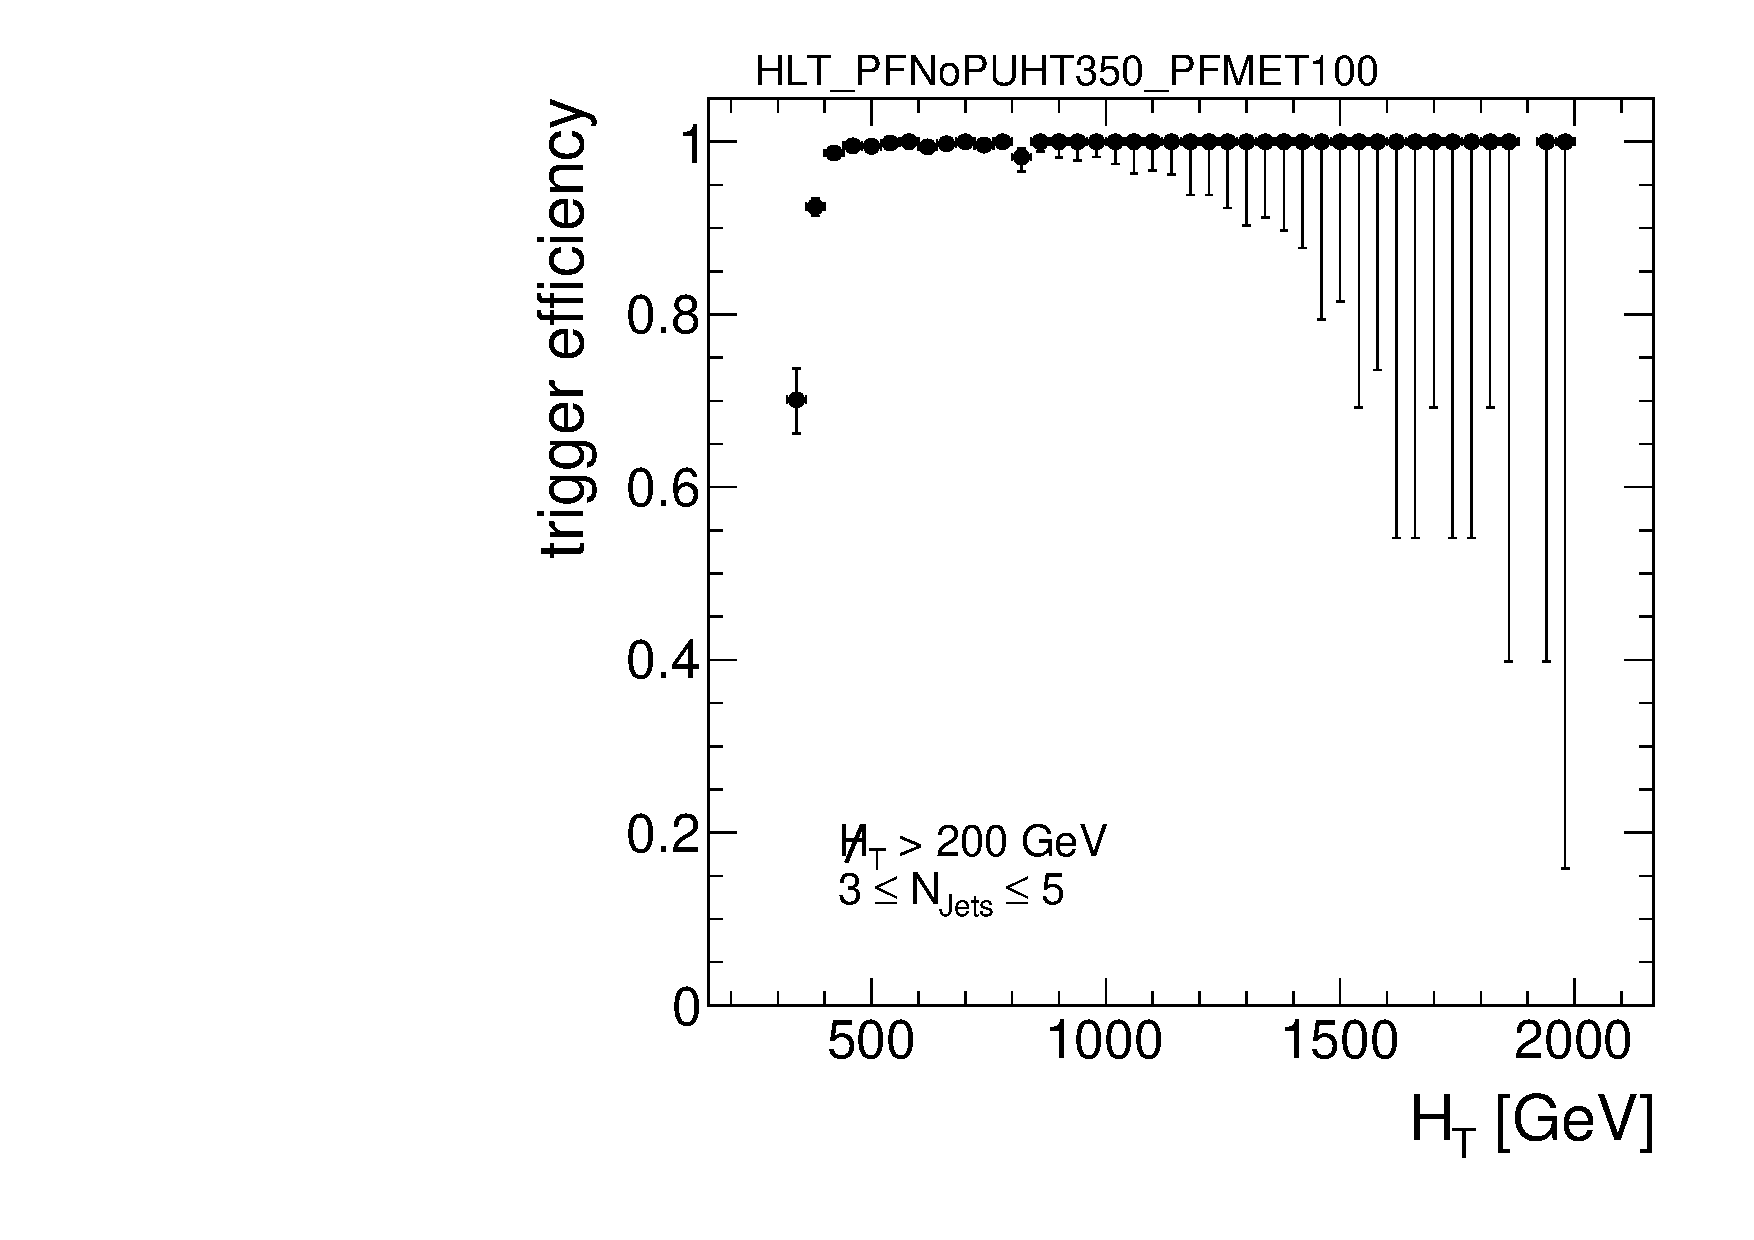
\includegraphics[width=0.47\textwidth]{figures/turn_on_HT_TagEle27WP80_ProbePFNoPUHT350PFMET100_MHT200_chs_NJets3-5.pdf} &
                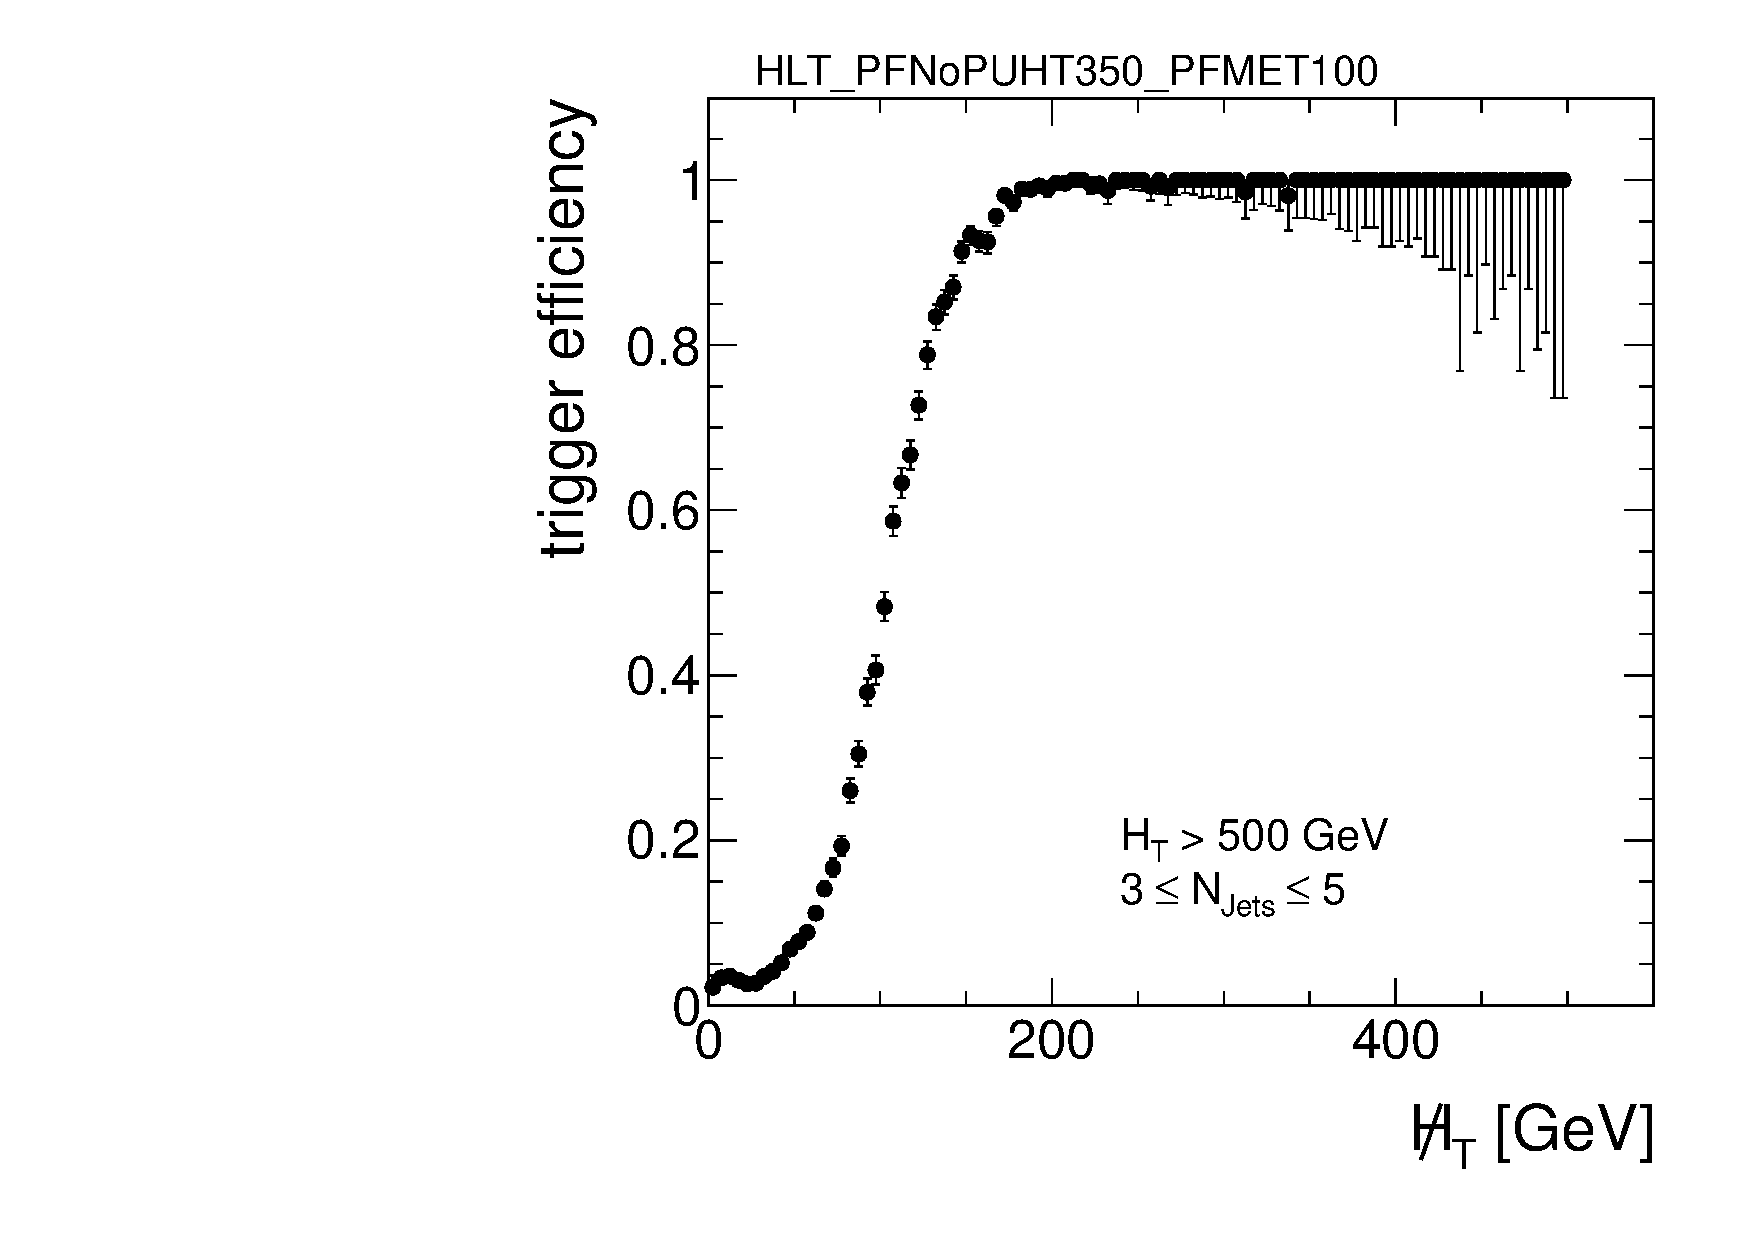
\includegraphics[width=0.47\textwidth]{figures/turn_on_MHT_TagEle27WP80_ProbePFNoPUHT350PFMET100_HT500_chs_NJets3-5.pdf} \\
  \end{tabular}
\caption{Measured relative trigger efficiency for paths HLT\_PFHT350\_PFMET100 (\textit{top}) and HLT\_PFNoPUHT350\_PFMET100 (\textit{bottom}) as a function of \HT (\textit{left}) and \MHT (\textit{right}) shown for $3 \leq$ \NJets $\leq 5$.} 
  \label{fig:trig_eff_3njets5}
\end{figure}
\begin{table}[!b]
  \caption{Summary of total trigger efficiencies of the signal triggers for selections of \HT$ > 500$\gev and \MHT$ > 200$\gev in different jet multiplicity intervals determined with respect to the reference trigger path.} 
  \label{tab:trig_eff}
  \begin{center}
    \begin{tabular}{lcc}
      \toprule
      \NJets & HLT\_PFHT350\_PFMET100 &  HLT\_PFNoPUHT350\_PFMET100\\
      \midrule
      3--5   & $99.4 _{-0.3} ^{+0.2}$   & $99.8 _{-0.1} ^{+0.1}$\\
      6--7   & $99.1 _{-2.0} ^{+0.7}$   & $100.0 _{-0.6} ^{+0.0}$\\
      $\ge$ 8 & $100.0 _{-36.9} ^{+0.0}$ & $100.0 _{-10.9} ^{+0.0}$\\
      \bottomrule
    \end{tabular}
  \end{center}
\end{table}

\subsection{Event Cleaning}
\label{subsec:RA2_cleaning}
The analysis presented in this chapter relies on a precise measurement of the momentum imbalance in the event. In order to remove events with large values of fake missing momentum arising from detector noise, a dedicated sequence of cleaning filters is applied: 
\begin{description}
 \item{\textbf{Primary Vertex and Beam Halo:}} Only events with at least one high-quality primary vertex are considered in the analysis. A primary vertex is classified as good, if it has more than four associated tracks and is located within 24\,cm in $z$ and 2\,cm in $xy$ direction from the nominal interaction point (\textit{good-vertex filter}). In order to detect events in which protons from the beam interact with residual gas molecules in the beam pipe, the CSC subdetector is used to identify muons moving parallel to the beam and removing them accordingly (\textit{beam-halo filter}).
 \item{\textbf{Anomalous Calorimeter Signals:}} Some events are affected by particles hitting the readout electronics or other technical instrumentation and cause anomalous signals in the ECAL or HCAL. For instance, noise in the readout system can fake artifical energy deposits at random times. Such events are identified based on timing and pulse-shape information (\textit{HBHE noise filter}). Furthermore, two $5 \times 5 $ supercrystal regions in the EE have been observed to give anomalously high energies. They are removed by imposing selections on the deposited energy in the identified supercrystals (\textit{EE bad supercrystal filter}). In order to account for transparency losses in the ECAL crystals, the system is calibrated with a dedicated laser. However, in the data some crystals are observed which receive unphysically large corrections. Events affected by this unusually large ECAL laser correction factors are rejected (\textit{ECAL laser correction filter}). The HCAL is also monitored by a dedicated laser system. Sometimes the laser fires into the collision bunch-crossing resulting in unwanted signals. These events are removed according to an event list indicating the affected events (\textit{HCAL laser filter}). The jet reconstruction utilizes information from the HO. This is used as identifier of significant leakage beyong the HCAL barrel. However, events with anomalous energy deposits in the HO result in fake \MHT and have to be rejected. Thus, events in which the fraction of the momentum deposited in the HO is $> 40\%$ are removed (\textit{HO filter}).
 \item{\textbf{Dead ECAL Cells:}} Some single crystals in the ECAL are malfunctioning. These dead ECAL cells make up around $1\%$ in total and can be responsible for energy losses resulting in large values of fake-\MHT. Such events can be identified by using the separate trigger primitive information of the L1 trigger to determine how much energy was lost (\textit{TP filter}) or by using the energy of the cells surrounding the masked cells (\textit{BE filter}).
 \item{\textbf{Tracking Failure:}} In some events, the track reconstruction is observed to fail which manifests in large calorimeter energy deposits with lack of associated tracks. This can be caused, \eg by too many seed clusters or by collisions not taking place in the actual centre of the detector. Thus, the scalar sum of track momenta associated to the good vertices divided by \HT in the event has to be larger than 10\% (\textit{tracking failure filter}) and if at least ten tracks are present in the event, good-quality tracks have to be more than 25\% (\textit{beam-scraping filter}). In addition, events with misreconstructed muon momenta in the PF algorithm (\textit{inconsistent muon filter}) or events in which energy from energetic HCAL towers traversed by soft muons is wrongly associated to the muon momentum (\textit{greedy muon filter}) are rejected. Furthermore, events with coherent noise in the strip tracker can occur. These cause several clusters distributed across the whole detector and lead to the identification of fake tracks. Such events, in which the track reconstruction aborted, can be identified by comparing the number of pixel clusters to the number of strip clusters (\textit{many strip clusters filter}, \textit{too many strip clusters filter}, \textit{log error too many strip clusters filter}). Another failure of track reconstruction occurs sometimes when track seeds from the TOB and TEC are used. Thus, events are rejected, if a jet with number of charged hadrons above 200 is reconstructed within $0.9 < |\eta| < 1.9$ (\textit{TOB/TEC tracking filter}).
 \item{\textbf{Noise Induced Jets:}} In order to reject events with fake jets arising for instance from detector noise, events are discarded, if the energy of a jet with \pt$ > 30$\gev is composed of more than 95\% from PF photon candidates or more than 90\% from PF neutral hadron energy (\textit{PBNR filter}).
\end{description}

\subsection{Baseline Selection}
\label{subsec:RA2_baseline}
The physics objects used in the analysis are reconstructed with the PF algorithm. Jets are clustered from the particle-flow objects with the anti-$k_\mathrm{T}$ algorithm using $R = 0.5$. Furthermore, they are calibrated, as discussed in Sec.~\ref{subsec:jets_calib}, including residual correction factors for data. \\
The following \textit{baseline selection} criteria are used to define the event sample used for the analysis. This selection defines a validation region and provides a basis for tighter criteria.
\begin{itemize}
 \item{The number of jets (\NJets) is required to be $\ge 3$. \NJets is defined as the number of jets with $\pt > 50$\gev and $|\eta| < 2.5$. This requirement is imposed in order to select multijet events.}
 \item{The scalar sum of jet momenta (\HT) is required to be $\ge 500$\gev with 
\begin{equation*}
\HT = \sum_{\mathrm{jets}} \pt 
\end{equation*}
for all jets that have $\pt > 50$\gev and $|\eta| < 2.5$. This condition selects events with a large visible energy in the event indicating a high energy scale of the hard interaction.}   
 \item{The absolute value of the negative vectorial sum of the jet momenta (\MHT) is required to be $\ge 200$\gev with
\begin{equation*}
\MHT = |\MHTvec|= |- \sum_{\mathrm{jets}} \ptvec |
\end{equation*}
for all jets with $\pt > 30$\gev and $|\eta| < 5.0$. This selection reduces contributions from standard model processes where missing transverse momentum is expected to be small. In particular, QCD multijet background is suppressed. } 
 \item{In order to suppress events in which missing transverse energy is mainly arising from jet mismeasurements, as for QCD multijet events, it is required that \MHT is not aligned with any of the leading three jets and events with
\begin{equation*}
\Delta \phi(\mathrm{jet}_n, \MHT) > 0.5 \;\; \mathrm{for} \;\; n = 1,2 \;\; \mathrm{and} \;\; \Delta \phi(\mathrm{jet}_3, \MHT) > 0.3
\end{equation*} 
are selected. The value of 0.5 is chosen according to the jet distance parameter. However, this is reduced in case of the third jet in order to retain signal efficiency. }
 \item{Background contributions arising from \ttbar and \WJets events are reduced by rejecting events containing isolated electrons or muons with $\pt > 10$\gev. These are required to have a good quality track that can be associated with the primary interaction vertex~\cite{CMS-PAS-EGM-10-004, CMS-PAS-MUO-10-002}. The isolation is given as the scalar sum of transverse momenta of PF particles (except for the lepton itself) within a cone of radius $\Delta R = 0.3$ for the electron and $\Delta R = 0.4$ for the muon, respectively. It is required to be less than 15\% of the transverse momentum of the electron and less than 20\% of the transverse momentum of the muon.}
\end{itemize}
After the application of the baseline selection, 26909 events are selected in data without the application of event cleaning filters. When imposing in addition the cleaning sequence, 11753 events constitute the event sample in data used for the analysis. This corresponds to a cleaning efficiency of around 56\%. In simulated events, around 28\% of the QCD multijet sample are rejected by the filters after the baseline criteria while it is less than 4\% for other background contributions. \\
A comparison of the events selected by the baseline criteria, including cleaning filters, in data and simulation is shown in Fig.~\ref{fig:ra2_baseline_mc}. In general, a reasonable agreement between data and MC distributions is observed. Especially in the bulk of the distributions, deviations are only at the order of 10--20\%. However, the background estimation from simulation is not further used in the analysis, but is meant to give an impression of the relative background contributions. Since the analysis is performed in extreme tails of the \HT, \MHT and \NJets phase space with only few events and large uncertainties in the simulation, SM background contributions are estimated solely with data-based methods.

\begin{figure}[!t]
  \centering
  % \makebox[\linewidth]{
  \begin{minipage}[c]{1.\textwidth}
    \begin{center}
      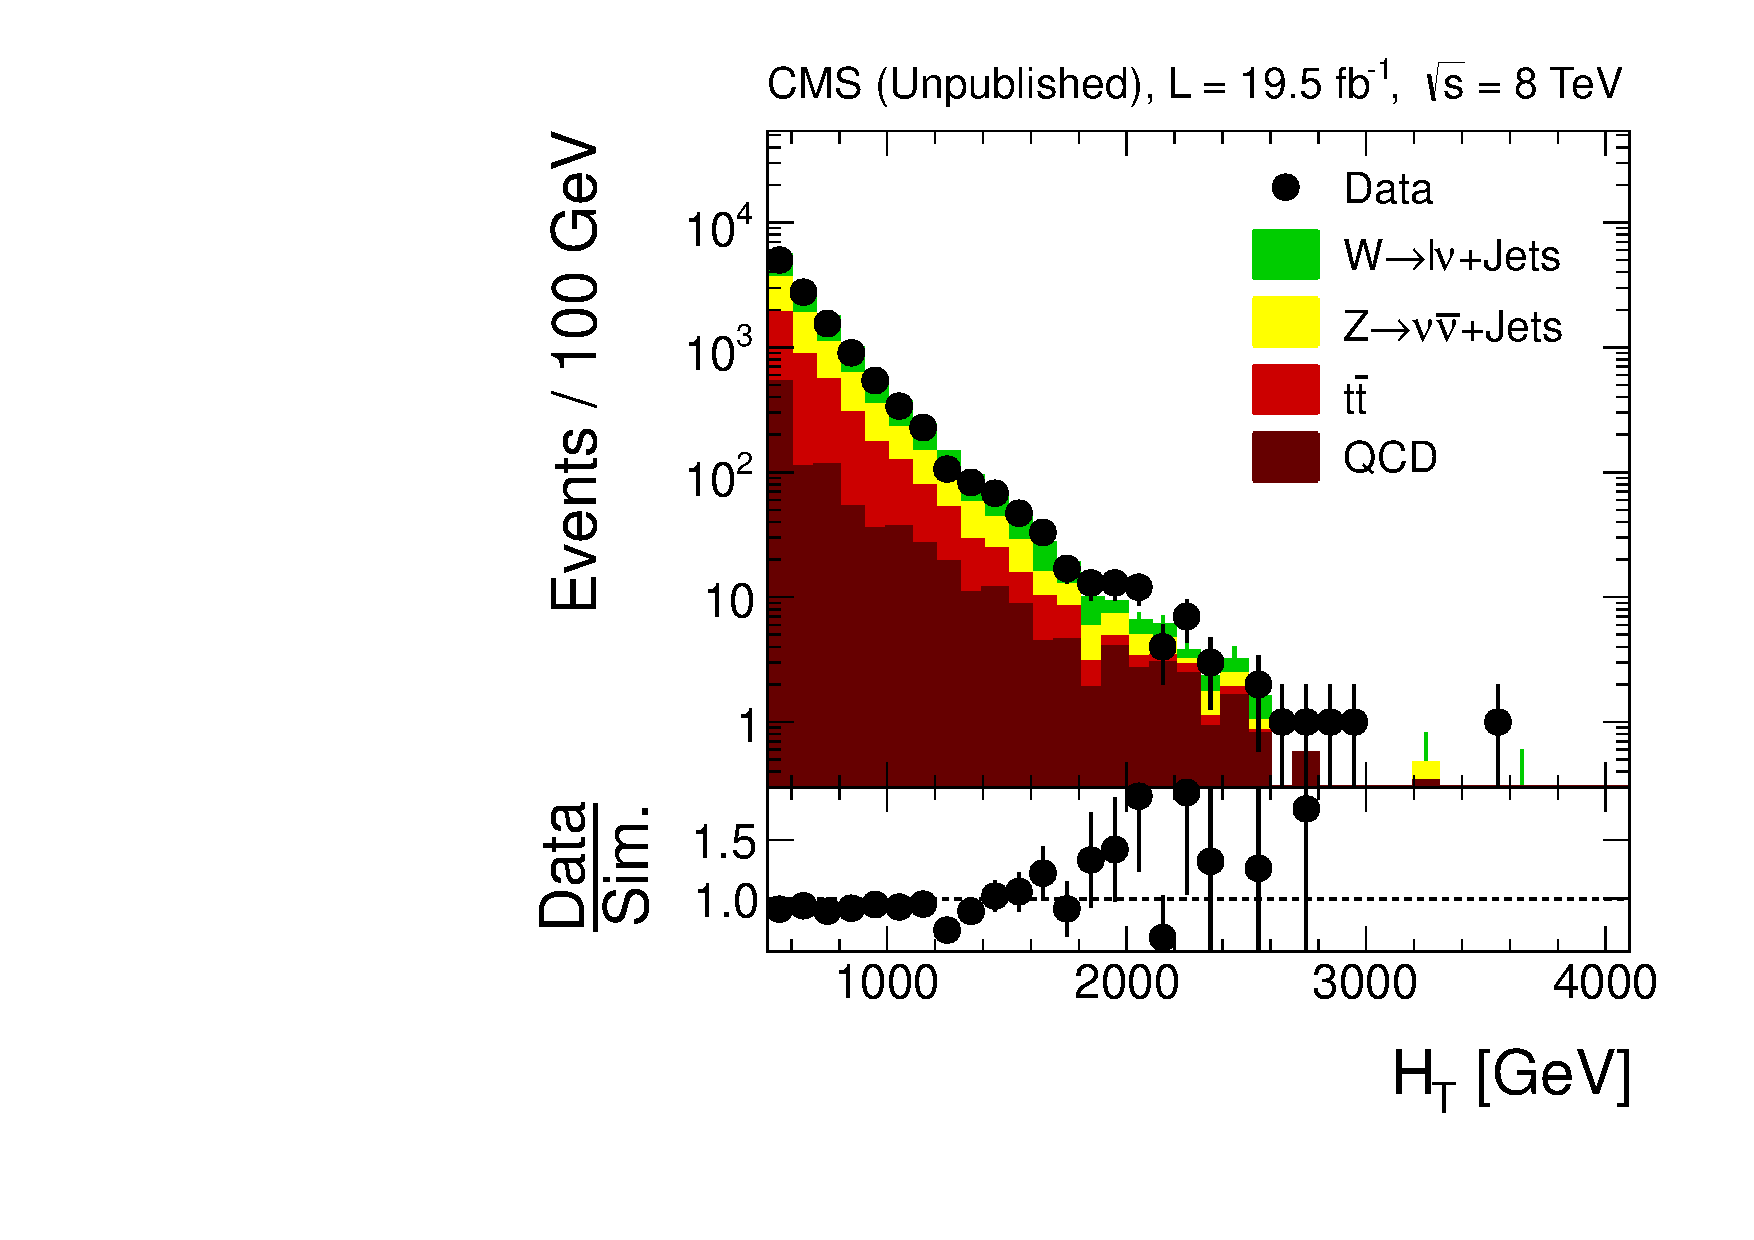
\includegraphics[width=0.49\textwidth]{figures/RA2_baseline_MC_HT.pdf}  
      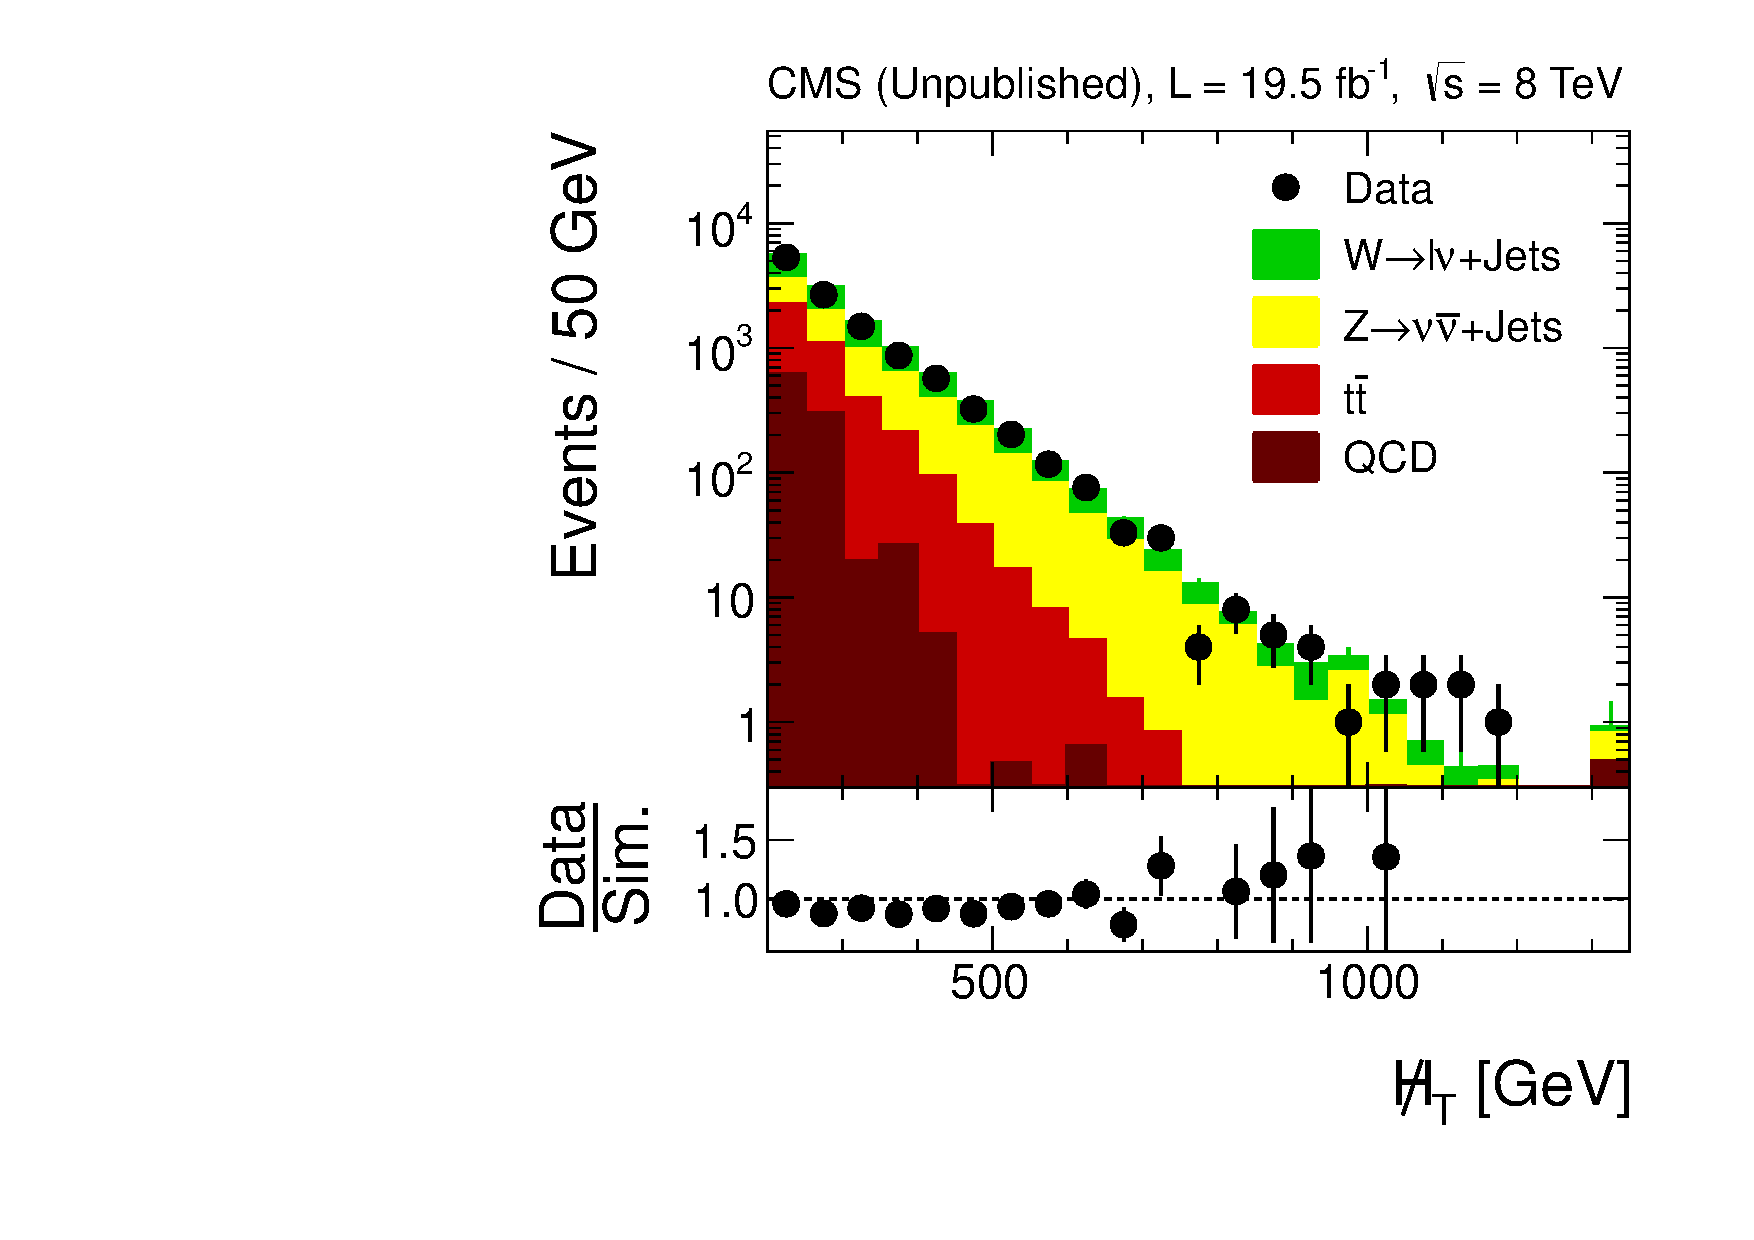
\includegraphics[width=0.49\textwidth]{figures/RA2_baseline_MC_MHT.pdf} \\
      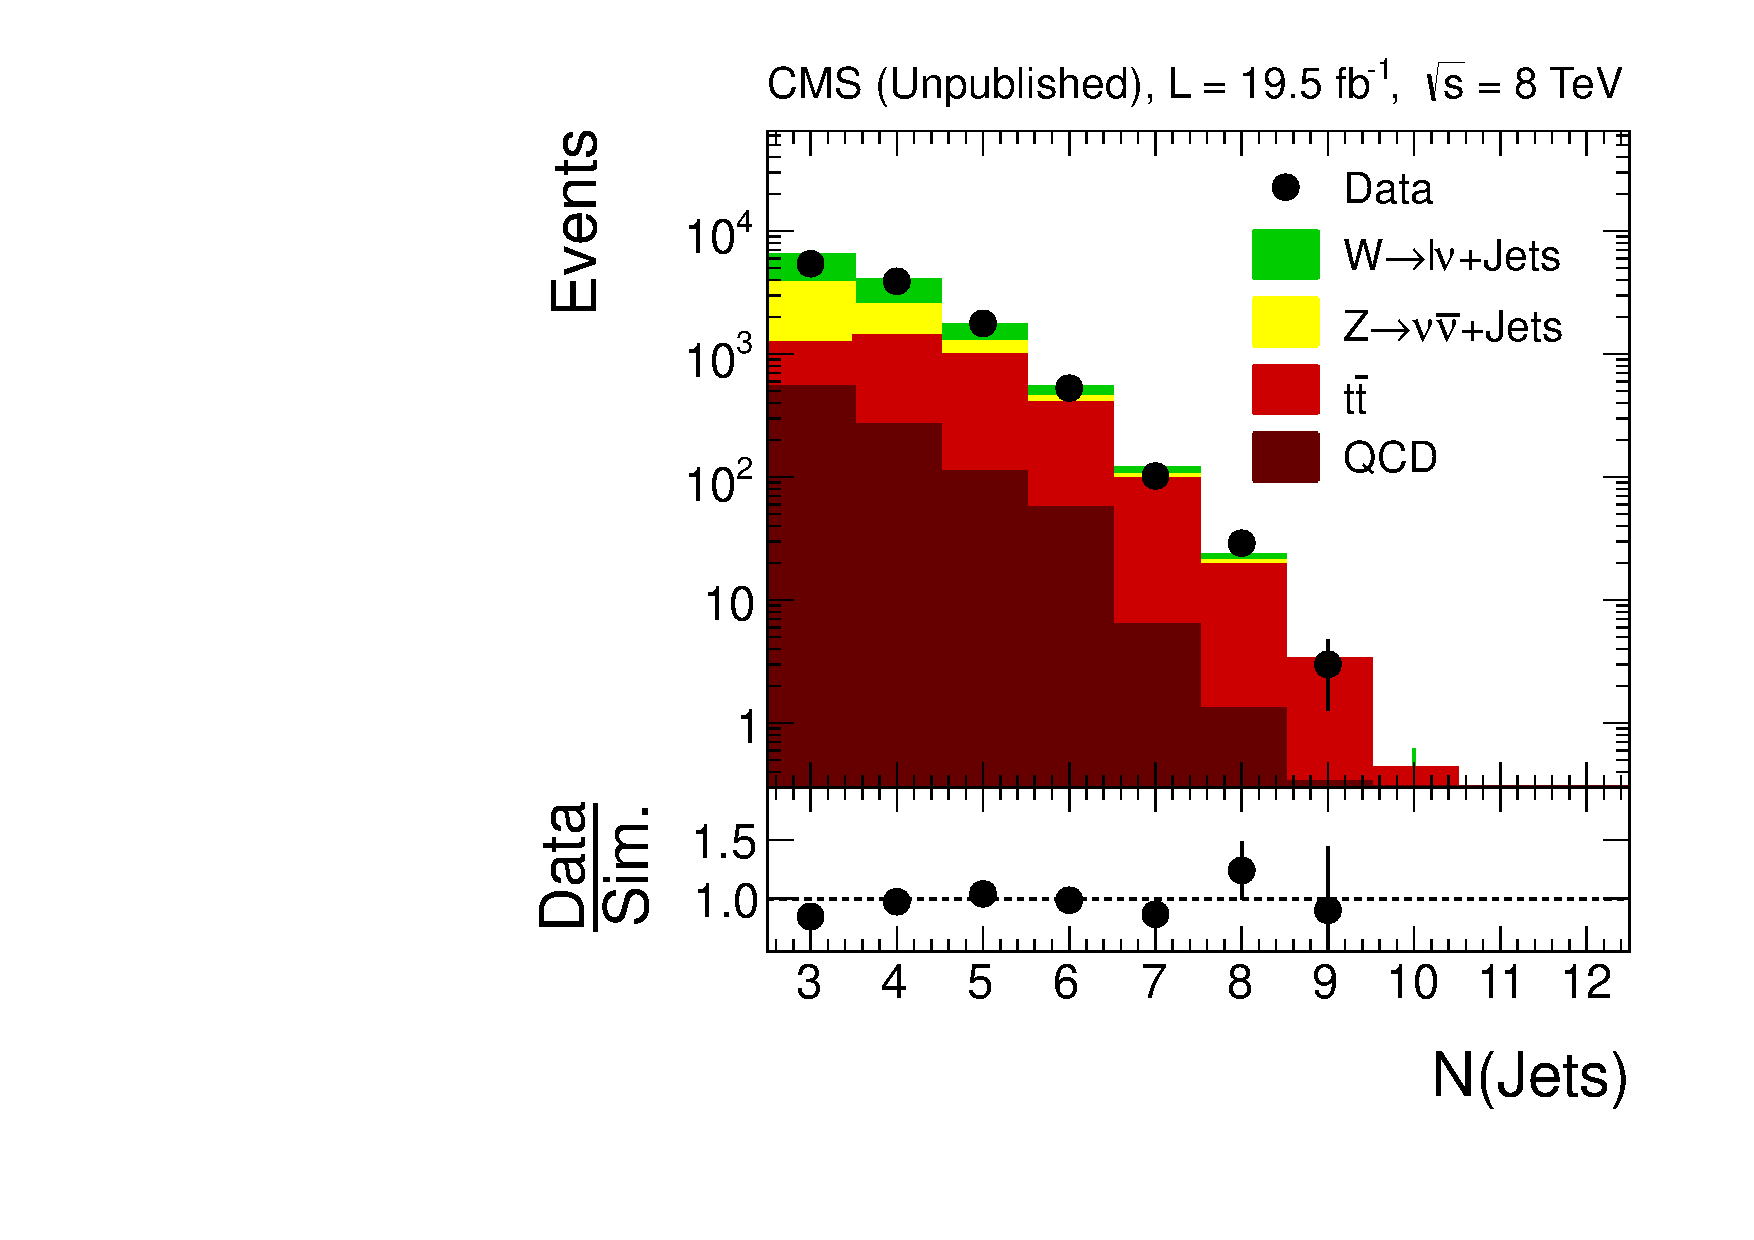
\includegraphics[width=0.49\textwidth]{figures/RA2_baseline_MC_NJets.pdf}
    \end{center}
  \end{minipage}

  \caption{Comparison of selected \HT (\textit{top left}), \MHT (\textit{top right}) and \NJets (\textit{bottom}) distributions in data (\textit{black dots}) and simulated events (\textit{shaded curve}) found from applying the event cleaning and baseline selection criteria described in Sec.~\ref{subsec:RA2_cleaning} and~\ref{subsec:RA2_baseline}. Only statistical uncertainties are shown. Taken from~\cite{Chatrchyan:2014lfa}.}
  \label{fig:ra2_baseline_mc}
\end{figure}

\subsection{Exclusive Search Regions}
\label{subsec:RA2_search_regions}
As mentioned in the beginning, the analysis presented in this chapter is an extension of previous inclusive searches. These were based on the requirement of at least three jets in the final state. In this analysis, the data are further subdivided into three exclusive jet multiplicity categories: $3 \leq \NJets \leq 5, 3 \leq \NJets \leq 5, \NJets \ge 8$. This enhances the sensitivity of the search towards multijet final states. These are typically the manifestations of long cascade decays from squarks and gluinos. Furthermore, it improves the sensitivity of the analysis to models in which gluinos often decay into top quarks. By requiring a large number of jets, this analysis utilizes a complementary approach to other analyses which often use the presence of bottom-quark jets in the final state to discriminate against background~\cite{Chatrchyan:2013lya, Chatrchyan:2013wxa, CMS-PAS-SUS-13-019, CMS-PAS-SUS-14-011}. \\
In order to gain sensitivity to a variety of models, the jet categories are further classified according to \HT and \MHT. With this approach, various exclusive search regions are defined. An overview of the exact definition of all 36 exclusive regions in \NJets, \HT and \MHT is given in Tab.~\ref{tab:excl_search_bins}.
\begin{table}[!t]
%\fontsize{10 pt}{1.2 em}
%\selectfont
\centering
\caption{Exclusive search regions used in the analysis binned in \HT, \MHT and \NJets.}
\begin{tabular}{lccc}
\multicolumn{4}{c}{} \\
  \toprule
   \NJets & [3-5] & [6-7] & [$\geq$8]  \\
  \midrule
             & \MHT [GeV]  & \MHT[GeV]  & \MHT[GeV]       \\
  \midrule
   500 $<$ \HT [GeV] $<$ 800   & 200--300 & 200--300 & $>$ 200 \\
                     & 300--450 & 300--450 &        \\
                     & 450--600 & $>$ 450  &        \\
                     & $>$ 600 &         &        \\
  \midrule
   800 $<$ \HT [GeV] $<$ 1000  & 200--300 & 200--300 & $>$ 200 \\
                     & 300--450 & 300--450 &        \\
                     & 450--600 & $>$ 450  &        \\
                     & $>$ 600 &         &        \\
  \midrule
   1000 $<$ \HT [GeV] $<$ 1250 & 200--300 & 200--300 & $>$ 200 \\
                     & 300--450 & 300--450 &        \\
                     & 450--600 & $>$ 450  &        \\
                     & $>$ 600 &         &        \\
  \midrule
   1250 $<$ \HT [GeV] $<$ 1500 & 200--300 & 200--300 & $>$ 200 \\
                     & 300--450 & 300--450 &        \\
                     & $>$ 450 & $>$ 450 &        \\
  \midrule
  \HT [GeV] $>$ 1500         & 200--300 & 200--300 & $>$ 200 \\
                     & $>$ 300  & $>$ 300  &        \\
  \bottomrule
\end{tabular}
\label{tab:excl_search_bins}
\end{table}    

\section{Estimation of Non-QCD Backgrounds}
\label{sec:RA2_Non-QCD}
As discussed in Sec.~\ref{subsec:susy_collider}, events from the SM processes \ZInvJets, \WJets or semi-leptonic \ttbar events (in which either the lepton is lost or a hadronically decaying $\tau$ lepton) and mismeasured QCD multijet events constitute important background contributions to all-hadronic final states. In this analysis, dedicated data-based methods are employed to estimate their size in the selected data. \\
In this section, those data-based background estimation methods are described. First, the estimation of non-QCD backgrounds (Sec.~\ref{subsec:RA2_Zinv}, Sec.~\ref{subsec:RA2_tauhad} and Sec.~\ref{subsec:RA2_lostlepton}) is reviewed. This is followed by a detailled discussion of the QCD background estimation (Sec.~\ref{subsec:RA2_QCD}). 

\subsection{Invisible Z Background}
\label{subsec:RA2_Zinv}
\begin{figure}[!t]
  \centering
\makebox[\linewidth]{
  \begin{tabular}{cc}
                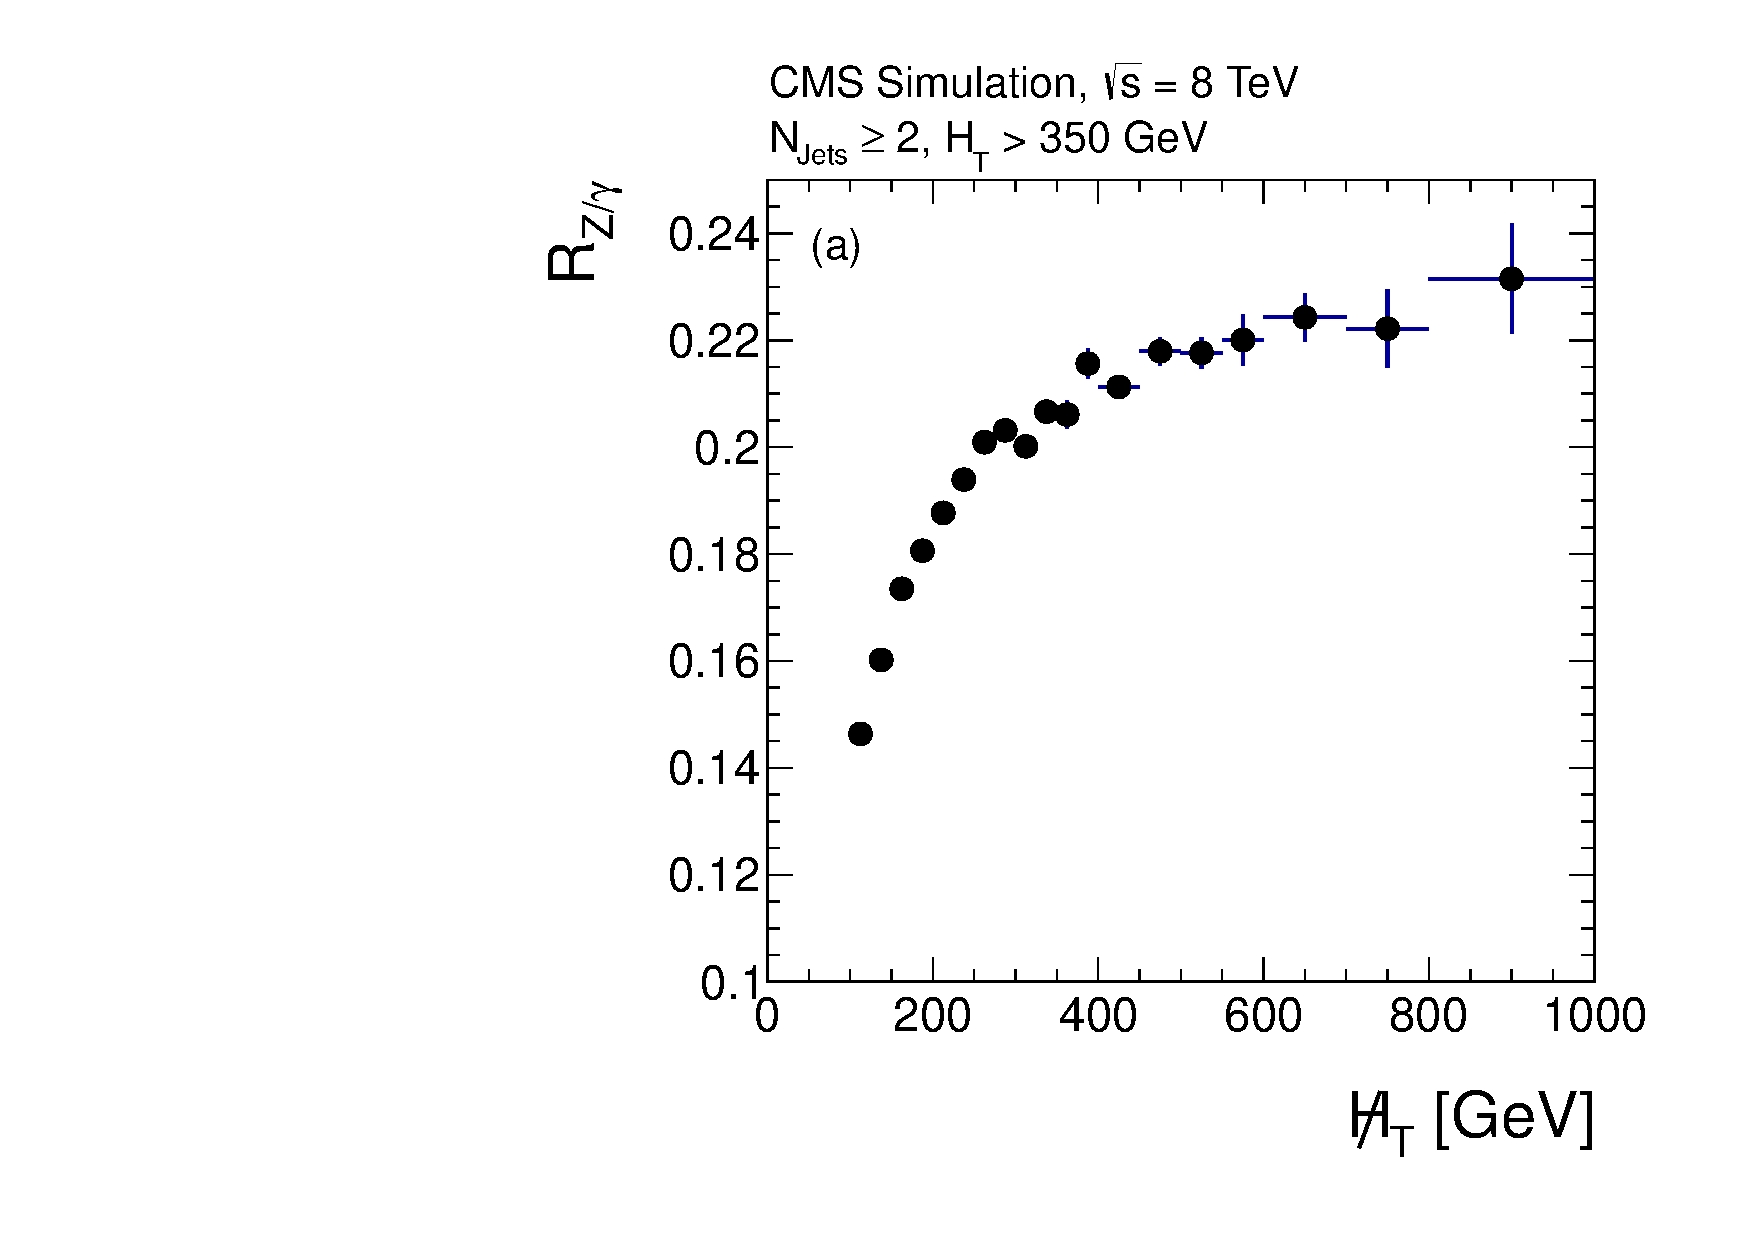
\includegraphics[width=0.49\textwidth]{figures/RA2_Zinv1.pdf} & 
                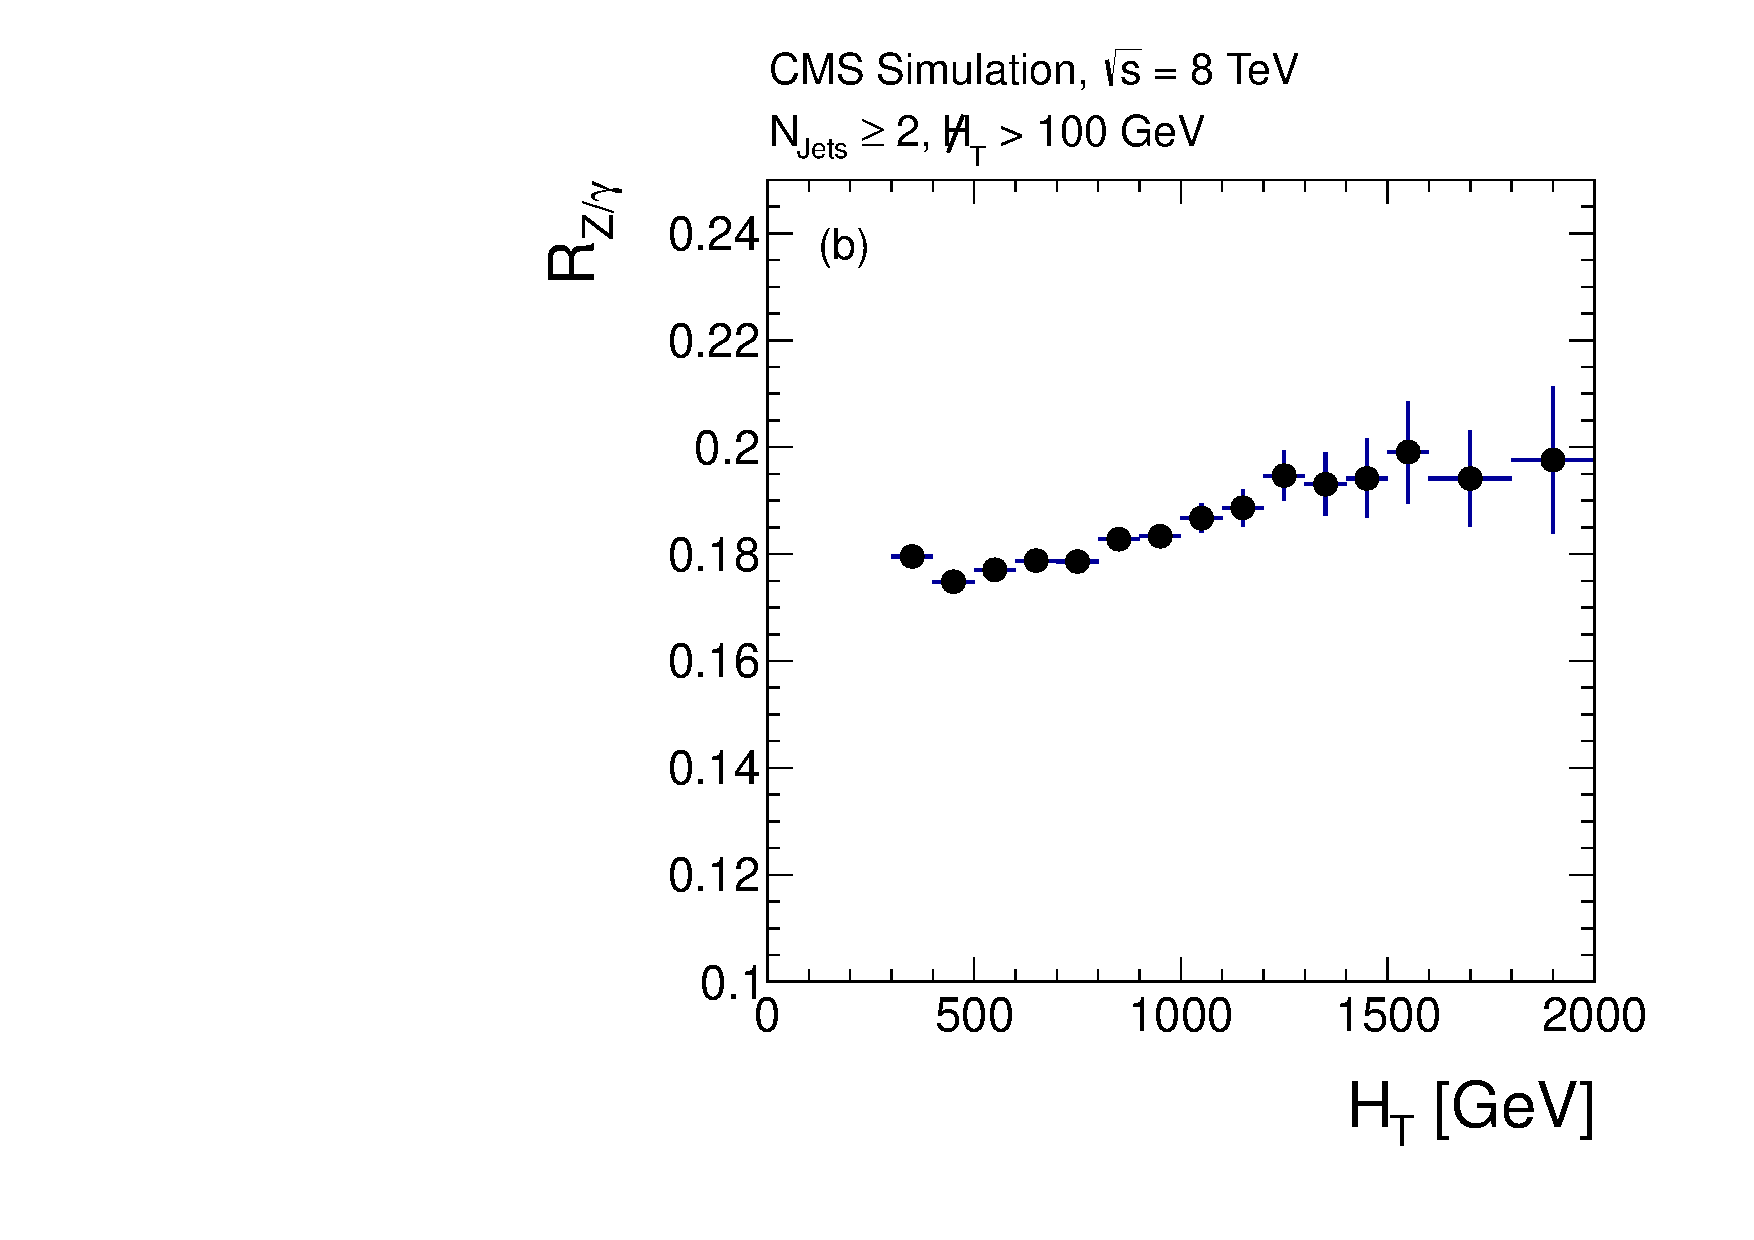
\includegraphics[width=0.49\textwidth]{figures/RA2_Zinv2.pdf} \\
                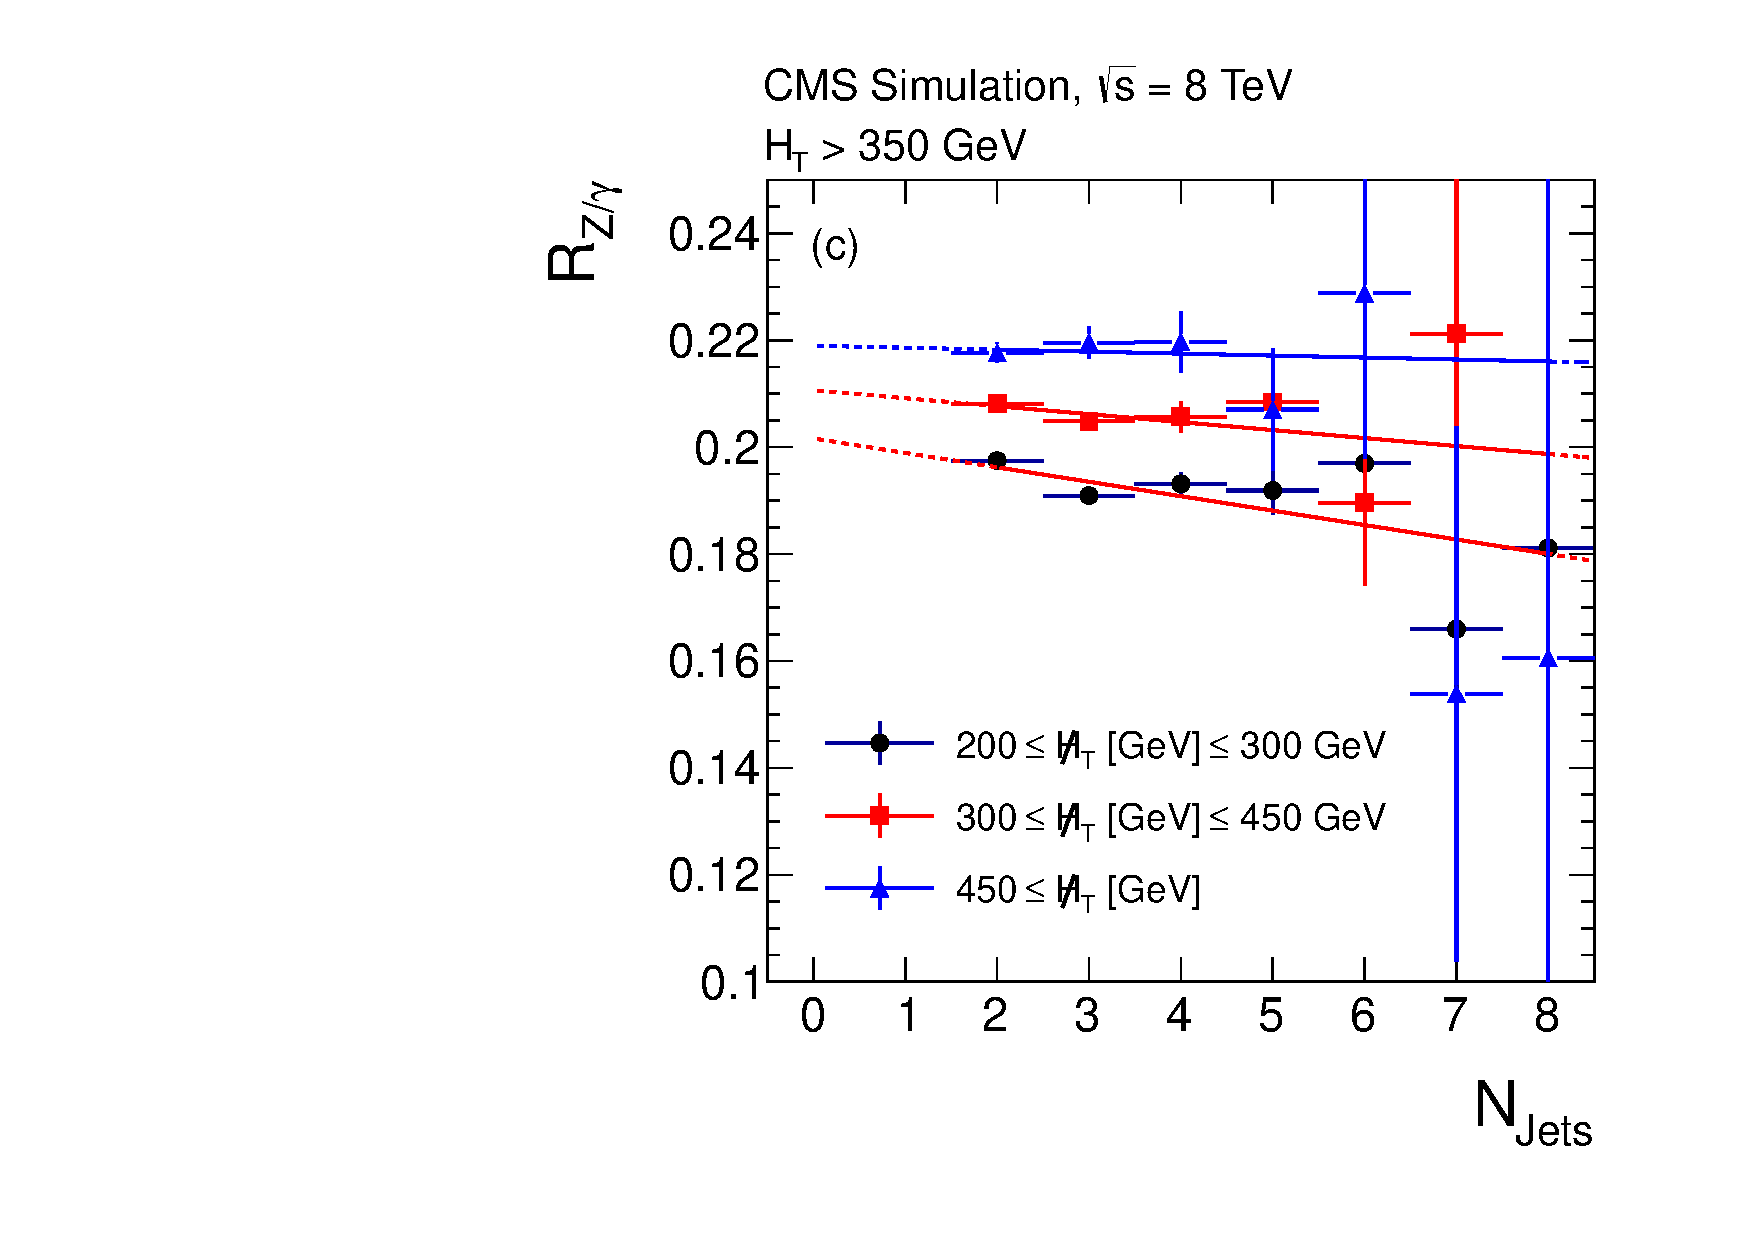
\includegraphics[width=0.49\textwidth]{figures/RA2_Zinv3.pdf} &
                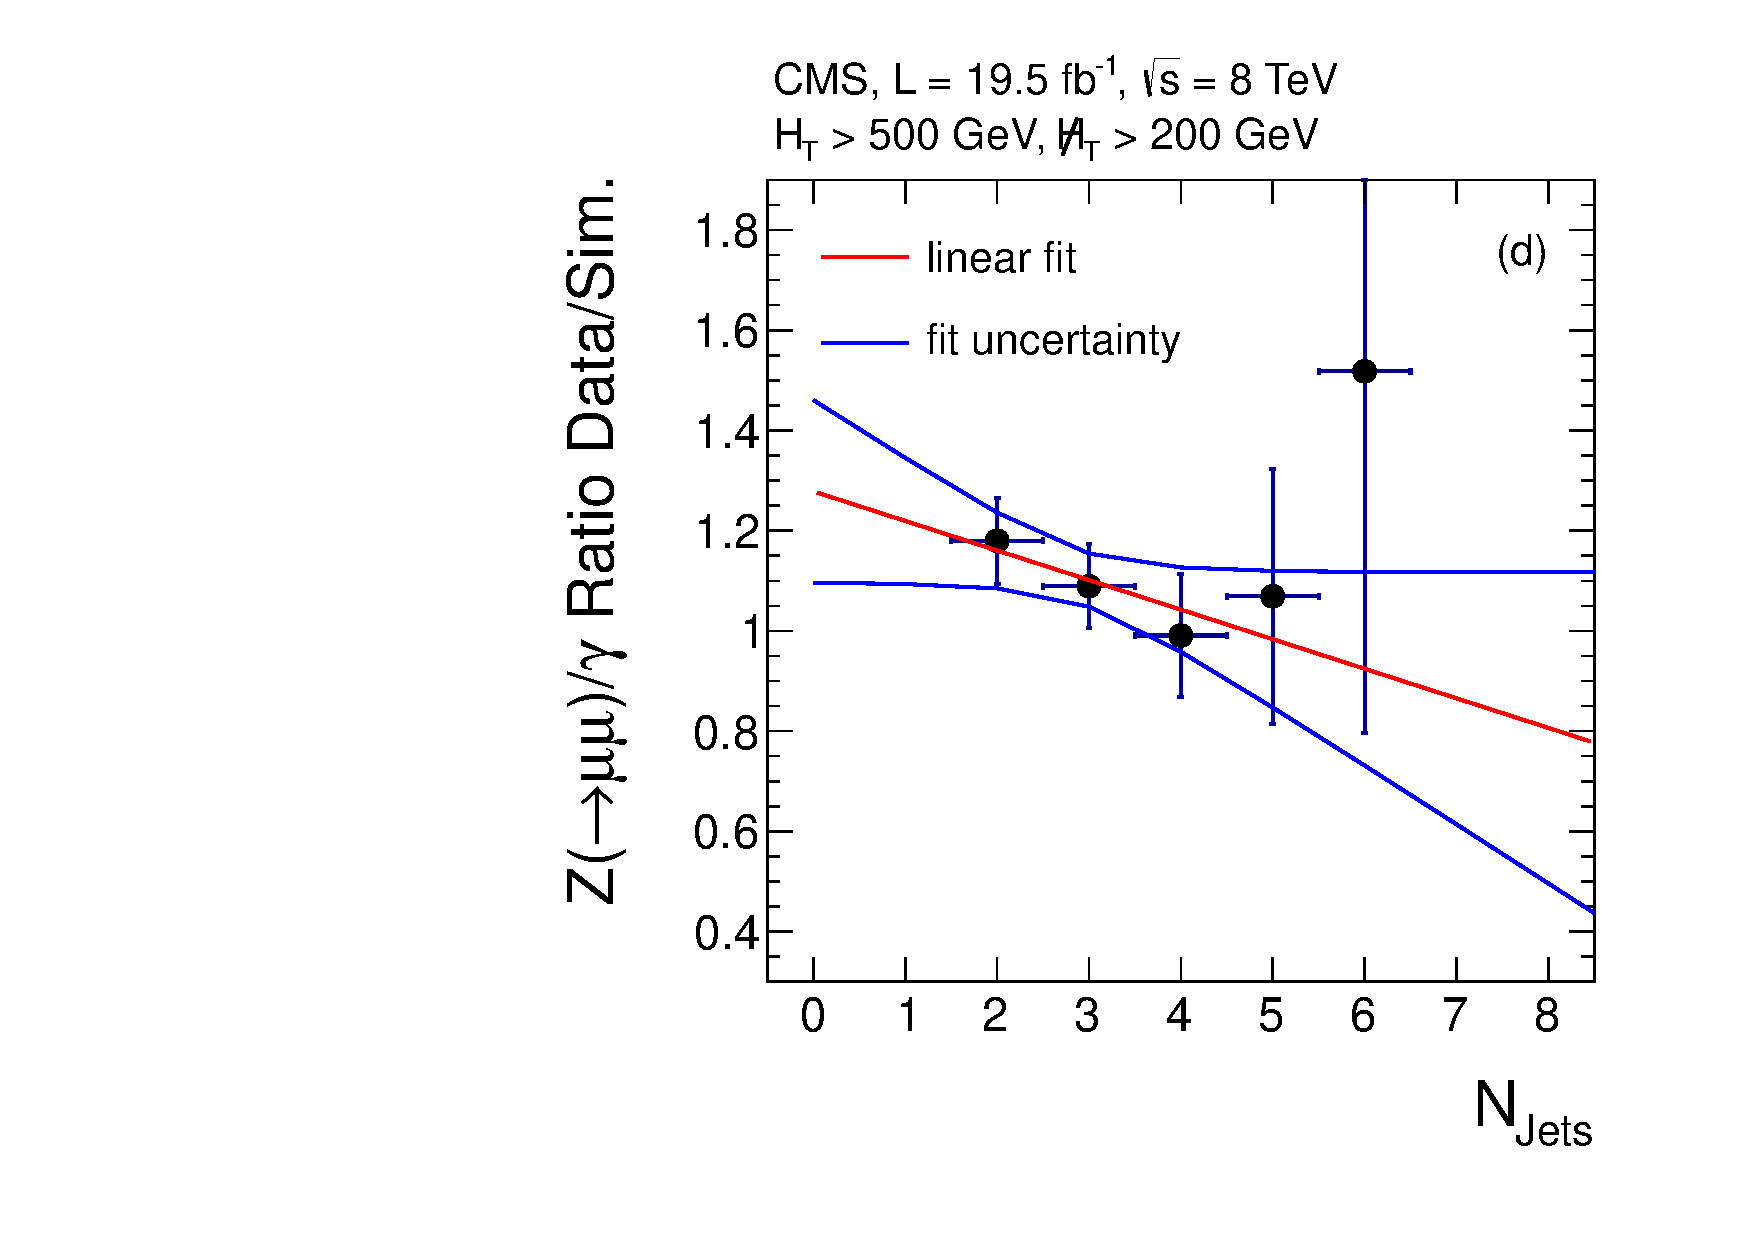
\includegraphics[width=0.49\textwidth]{figures/RA2_Zinv4.pdf}
  \end{tabular}}
  \caption{The simulated ratio $R_{Z/\gamma}$ as a function of (a) \MHT, (b) \HT, (c) \NJets, where the values for three \MHT selections are shown with linear fits, and (d) the double ratio of $R_{Z(\mu\mu)/\gamma}$, using events from data to those from simulation; the linear fit and its uncertainty band are overlaid~\cite{Chatrchyan:2014lfa}.}
  \label{fig:ra2_zinv}
\end{figure}
The irreducible background contributions arising from \ZInvJets events are estimated using \photonJets events. This is a well suited method as for high transverse momenta of the vector boson the event kinematics are the same and the cross sections differ mainly according to the different boson-quark couplings~\cite{Ask:2011xf, Bern:2012vx}. \\
The \photonJets sample is collected by triggering on a $\photon$ candidate and large values of \HT. Photon candidates are selected, if they satisfy \pt$ > 100$\gev and $|\eta| < 1.44$ or $1.566 < |\eta| < 2.5$. Furthermore, they have to have a shower profile consistent with that of a prompt photon produced directly in the hard interaction. In order to distinguish photons from misidentified electrons they must not have an associated track in the pixel detector. In addition, photon candidates are required to be isolated meaning that in a cone of radius $\Delta R = 0.3$ the summed transverse momenta of PF candidates around the momentum direction of the photon candidate are not allowed to exceed a certain value. The number of selected \photonJets events is corrected for photon acceptance, reconstruction and isolation efficiency. Furthermore, the purity of the \photonJets sample, which is the fraction of selected photon candidates emerging from direct production, has to be taken into account. The number of background photons caused for instance by misidentified jet fragments, is estimated by exploiting the difference between the shower profile of prompt and background photons. The average purity of the \photonJets sample is measured to be 93\%. Subsequently, the number of \ZInvJets events in data $N_{\ZInvJets}^{\text{data}} (\HT, \MHT, \NJets)$ using the number of selected \photonJets events $N_{\photonJets}^{\text{data}} (\HT,\MHT,\NJets)$ is obtained according to
\begin{equation*}
N_{\ZInvJets}^{\text{data}} (\HT, \MHT, \NJets) = R^{\text{MC}}_{Z(\nu\bar{\nu})/\gamma} (\HT,\MHT,\NJets)
                                                        \times 
                                                       N_{\photonJets}^{\text{data}} (\HT,\MHT,\NJets)
                                                       \times 
                                                       \frac{R_{Z(\mu\mu)/\gamma}^{\text{data}}}{R_{Z(\mu\mu)/\gamma}^{\text{MC}}}
\label{eqn:photoncorr}
\end{equation*}
with the ratio relating the production cross section of \ZInvJets and \photonJets events $R^{\text{MC}}_{Z(\nu\bar{\nu})/\gamma} (\HT,\MHT,\NJets)$ determined in simulation and the double ratio $\frac{R_{Z(\mu\mu)/\gamma}^{\text{data}}}{R_{Z(\mu\mu)/\gamma}^{\text{MC}}}$ selected in data and MC to account for theoretical uncertainties on $R_{Z/\gamma}$ especially for high jet multiplicities~\cite{Bern:2012vx, Bern:2011pa}. The missing momentum in the event is emulated by ignoring the momentum of the photon candidate in the calculation of \MHT. \\
The behaviour of $R_{Z/\gamma}$ is examined in simulated events as a function of \MHT, \HT and \NJets. The obtained distributions are shown in Fig.~\ref{fig:ra2_zinv}\,(a) -- (c). While a strong dependence on \MHT for small values ($\lesssim 500$\gev) is observed, the variation as function of \HT amounts to only $(12 \pm 5)\%$ in the relevant range for this analysis of $500 < \HT < 1500$\gev. The ratio as a function of the jet multiplicity is determined for different \MHT ranges, which are $200 < \MHT < 300$\gev, $300 < \MHT < 450$\gev and $\MHT > 450$\gev. The behaviour in each of these \MHT ranges is described by a linear function also displayed in Fig.~\ref{fig:ra2_zinv}\,(c). It is found that the ratio decreases slightly with increasing jet multiplicity which is consistent with findings from theory~\cite{Bern:2012vx, Bern:2011pa}. In order to take the theoretical uncertainty on $R_{Z/\gamma}$ obtained from simulated events into account, differences of this phenomenological ratio in data and simulated events are studied using $Z(\mu\mu)$ events. The double ratio of $R_{Z(\mu\mu)/\gamma}^{\text{data}}$ to $R_{Z(\mu\mu)/\gamma}^{\text{MC}}$ is derived as a function of the jet multiplicity and shown in Fig.~\ref{eqn:photoncorr}\,(d). It is fitted with a linear function, and the deviation from unity is considered as correction for the $R_{Z/\gamma}$ ratio in each jet multiplicity selection. \\
The main sources of uncertainty for the prediction of \ZInvJets events arise from the fit uncertainty to the double ratio which is at the order of 20\%, 25\% and 45\% for the different jet multiplicity intervals, the differences between data and simulation regarding the photon identification and isolation as well as the subtraction of background photons from QCD multijet events.

\subsection{Hadronic-tau Background}
\label{subsec:RA2_tauhad}
\begin{figure}[!t]
  \centering

  \begin{minipage}[c]{1.\textwidth}
    \begin{center}
      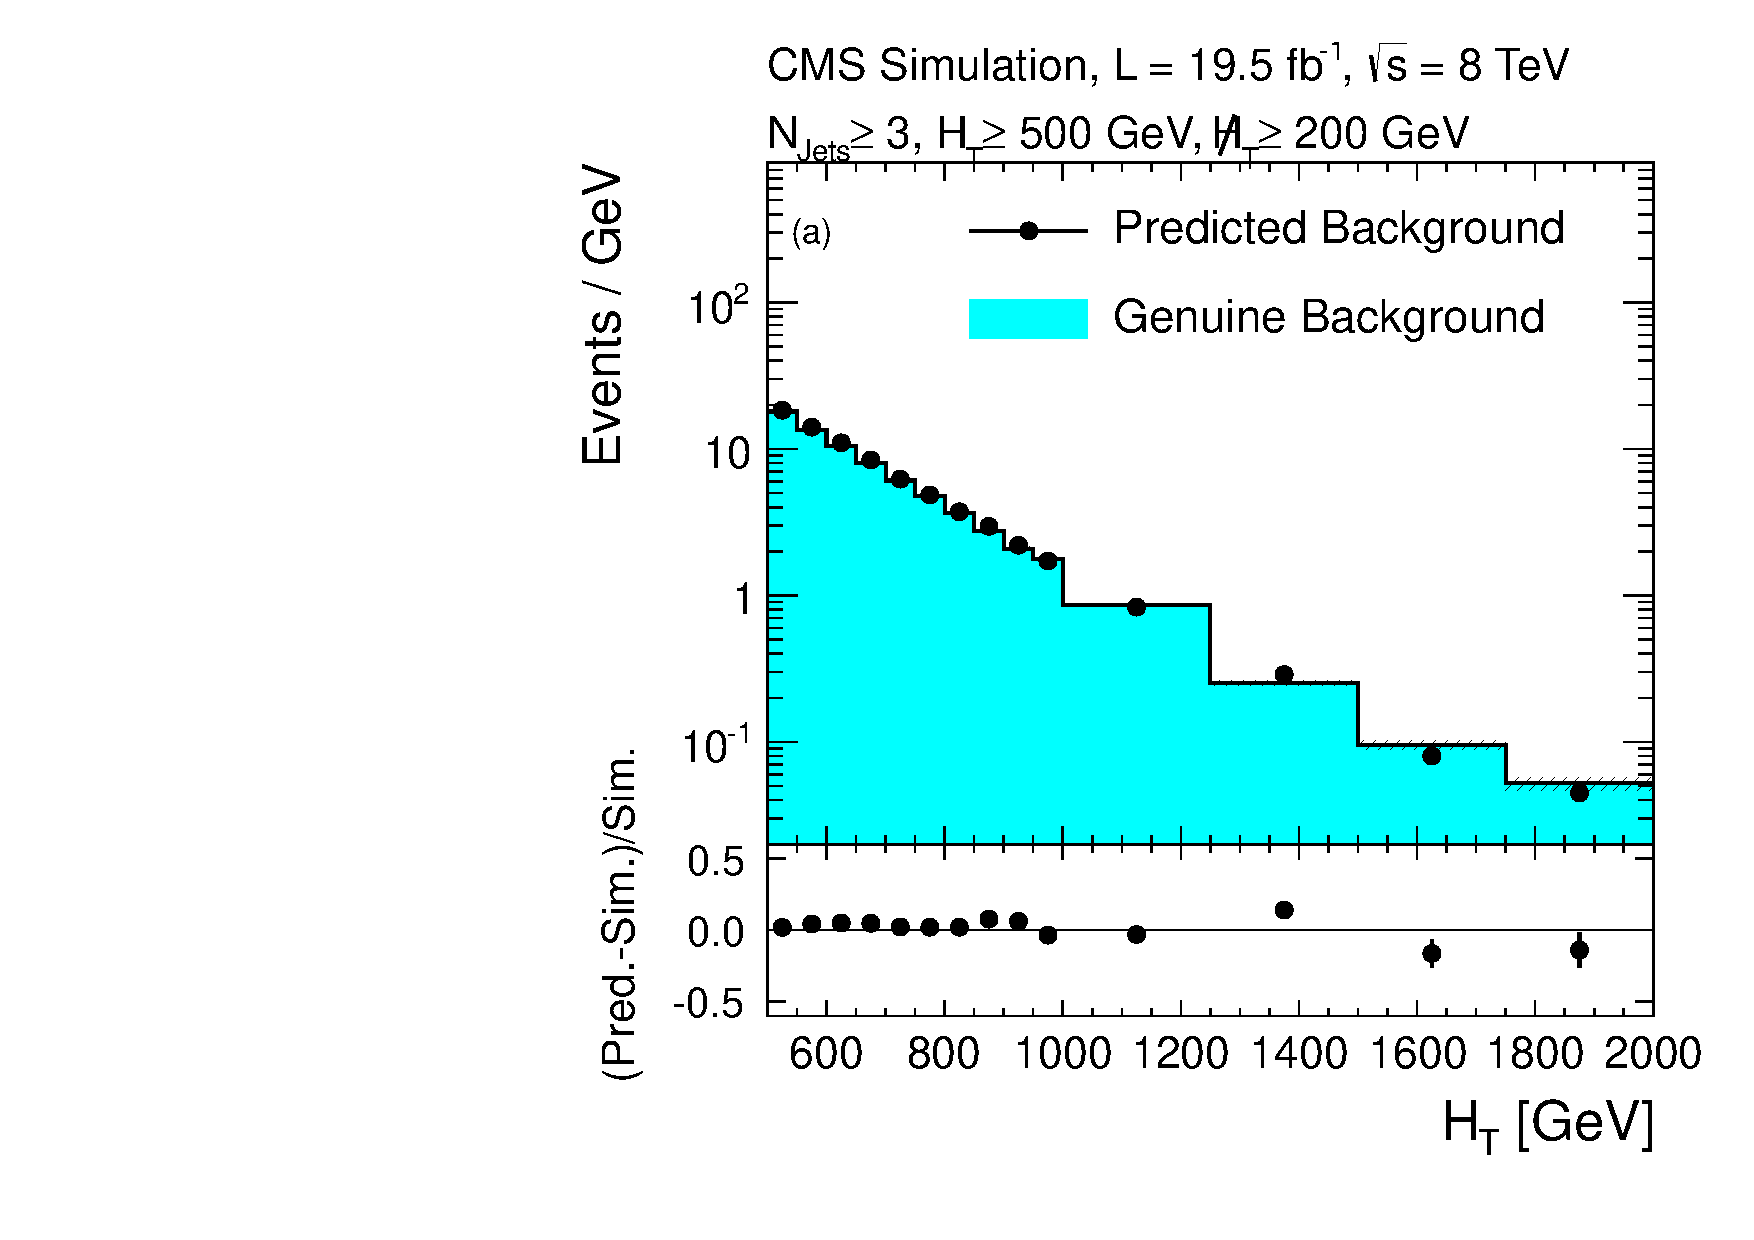
\includegraphics[width=0.49\textwidth]{figures/RA2_TauHad1.pdf}% \hspace {1.5 pt} 
      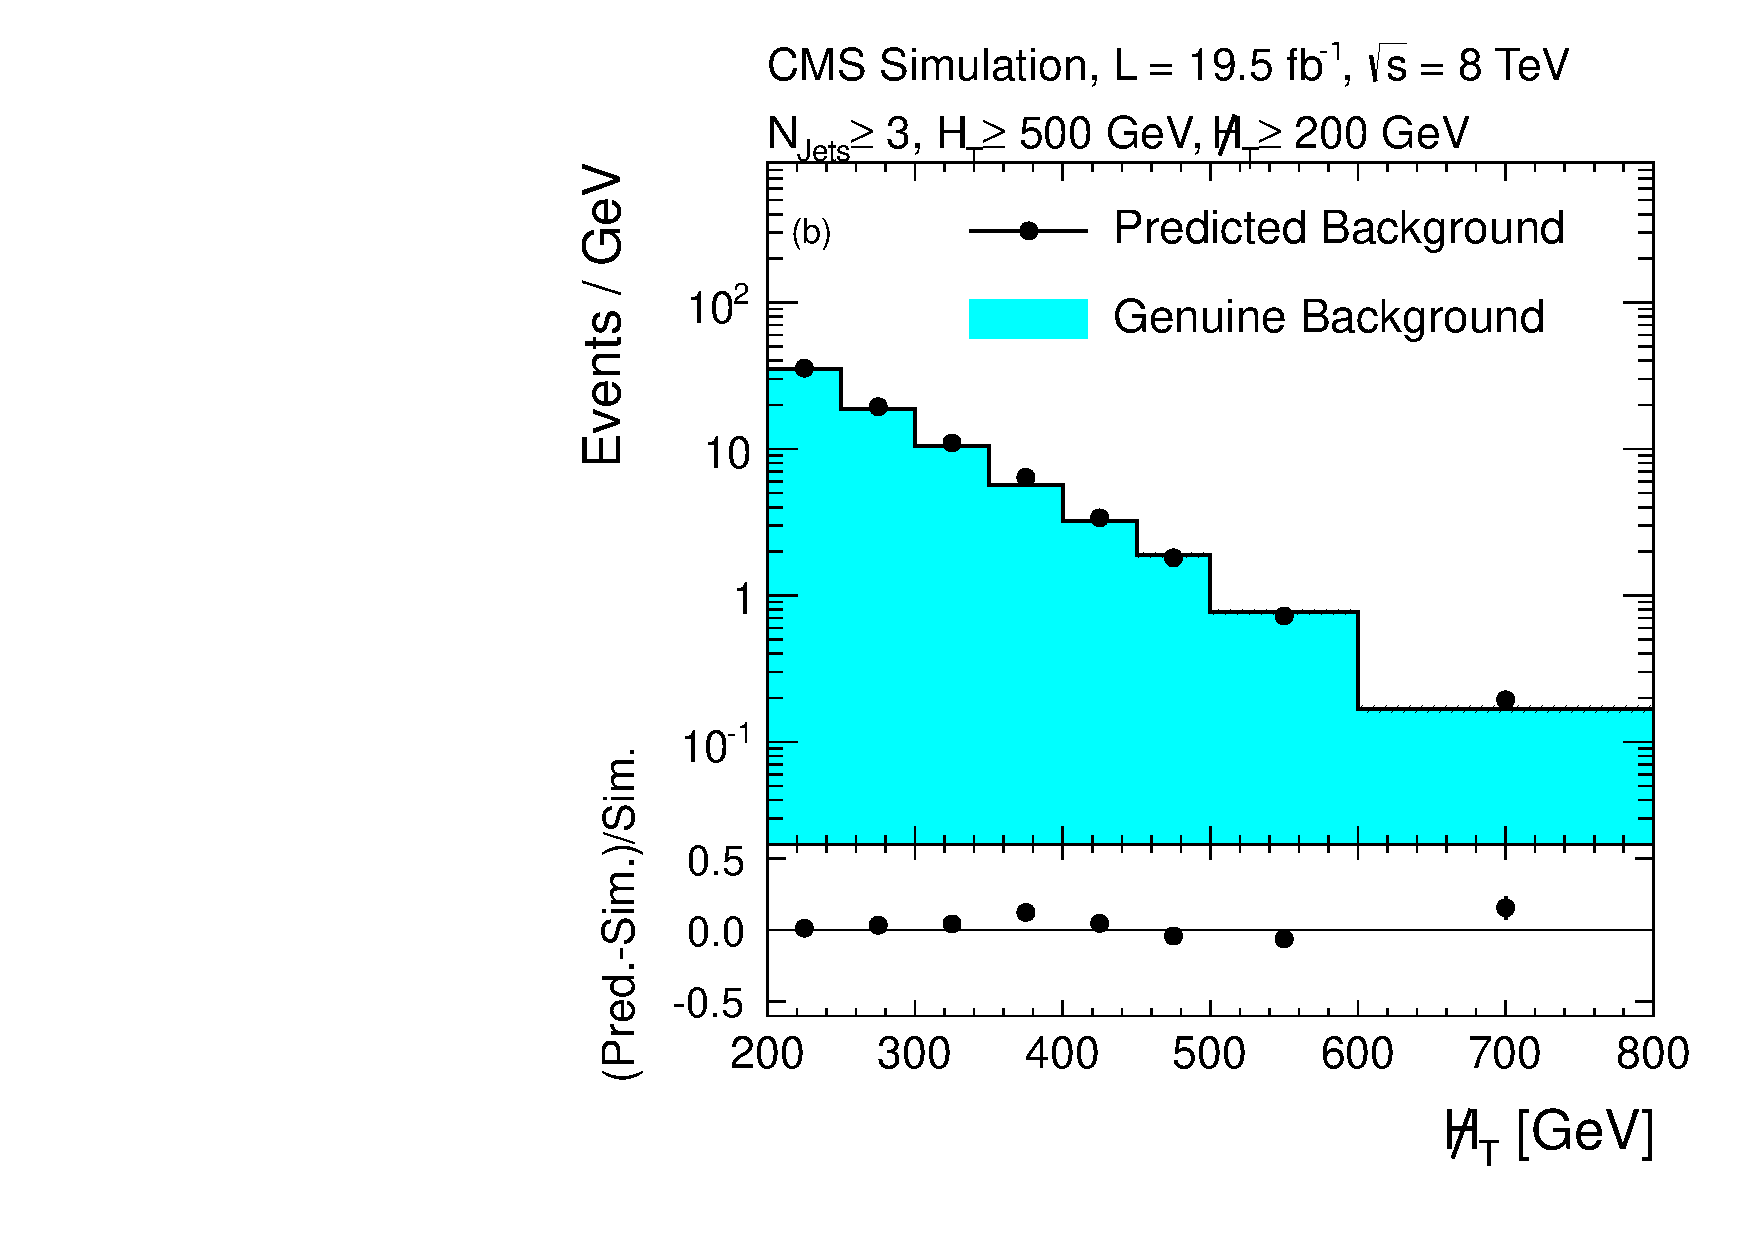
\includegraphics[width=0.49\textwidth]{figures/RA2_TauHad2.pdf}\\ 
      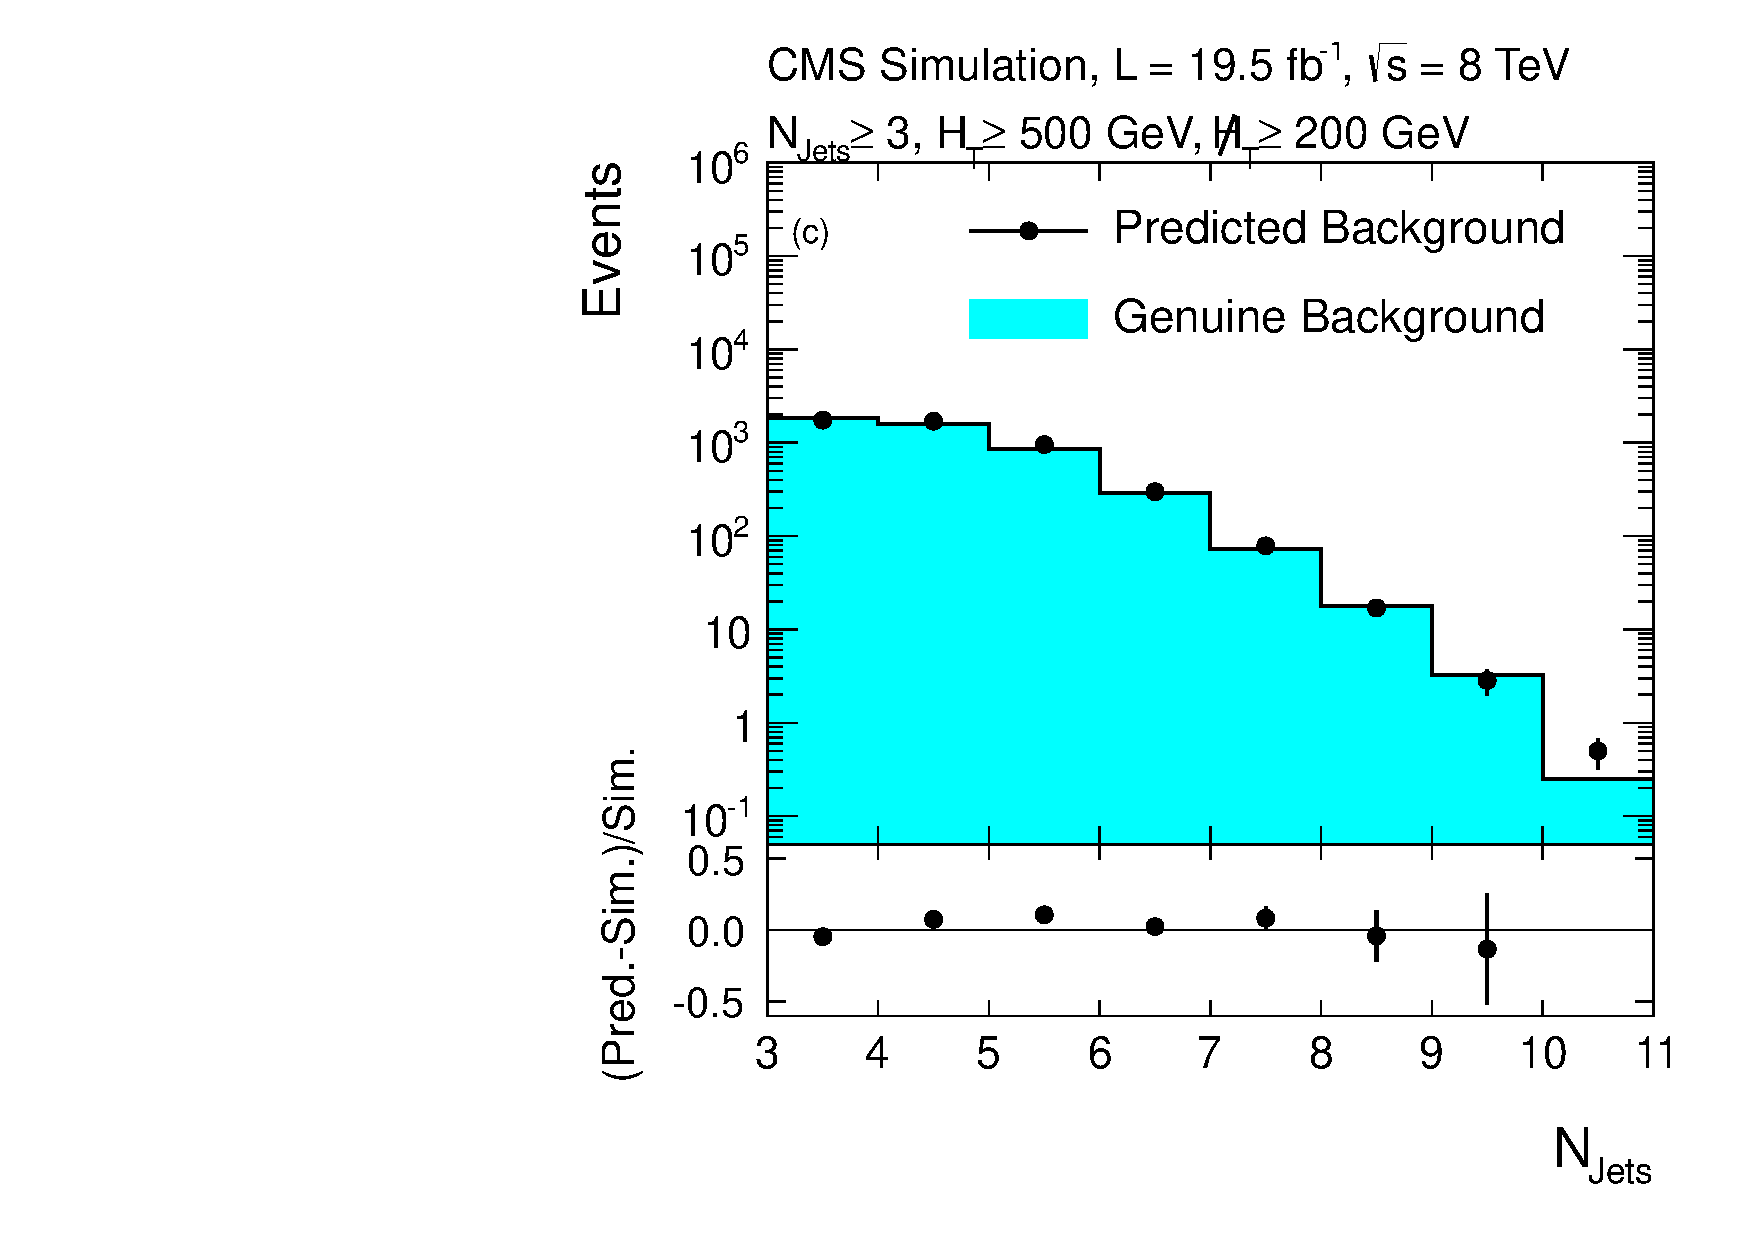
\includegraphics[width=0.49\textwidth]{figures/RA2_TauHad3.pdf}
    \end{center}
  \end{minipage}

  \caption{Predicted (a) \HT, (b) \MHT, and (c) \NJets distributions found from applying the hadronic-tau background evaluation method to simulated \ttbar and \WJets events (solid points) in comparison to the genuine \ttbar and \WJets background from simulation (shaded curve). Only statistical uncertainties are shown~\cite{Chatrchyan:2014lfa}.}
  \label{fig:ra2_tauhad}
\end{figure}
Background contributions arising from \WJets and \ttbar events with a hadronically decaying $\tau$ lepton are estimated using a $\mu + \mathrm{jets}$ control sample. Since $\mu + \mathrm{jets}$ and $\tau_h + \mathrm{jets}$ events arise from the same physics process, they feature the same kinematics except for the different response of the detector to a $\mu$ and a $\tau_h$.  \\
The $\mu + \mathrm{jets}$ sample is selected by triggering on a single isolated muon or a muon accompanied by at least two jets. Furthermore, instead of applying a lepton veto, exactly one $\mu$ with \pt$ > 20$\gev and $|\eta| < 2.1$ is required. In order to prevent the control sample from signal contamination, a selection on the transverse mass $m_\mathrm{T} = \sqrt{2\pt^{\mu}\met[1-\mathrm{cos(\Delta \phi)}]}$ of $m_\mathrm{T} \le 100$\gev is imposed with the azimuthal angle $\Delta \phi$ between the direction of the muon four-momentum and the \met vector. \\
The difference between the $\mu$ and the $\tau_h$ is taken into account by replacing the muon by a simulated $\tau_h$ jet. This is done by randomly sampling the transverse momentum of the $\tau_h$ jet from the response $\pt^\mathrm{jet}/\pt^{\tau}$, obtained from simulation, of a reconstructed jet with $\pt^\mathrm{jet}$ matched to a generated hadronically decaying $\tau$ lepton with $\pt^{\tau}$. Technically, sampling means that the four-momentum of the muon is scaled with the proper value from the $\tau_h$ response. However, if an event in the control sample is obtained from a prescaled trigger, the sampling is performed not only once but increased according to the prescale factor. For the calculation of the response, the generated $\tau$ lepton has to fulfill $\pt > 20$\gev and $|\eta| < 2.1$ and the distance for the matching is chosen to be $\Delta R < 0.2$ for tau-\pt$ < 50$\gev and $\Delta R < 0.1$ otherwise. The response is obtained from simulated \ttbar and \WJets events and subsequently mixed according to the cross sections of these processes. \\
In order to sample the complete response function, the random sampling of the response is repeated one hundred times for each event following a bootstrap method~\cite{GVK017474957}. The actual prediction is given by the mean of the set of predictions from the bootstrapping and the statistical uncertainty is obtained from the standard deviation. Furthermore, also the statistical uncertainty of the seed sample is taken into account by considering the number of occurences of a seed event in the signal region. \\
In the following, \HT, \MHT and \NJets are recalculated for each event, including the transverse momentum of the $\tau_h$ jet, and all selection criteria, as described in Sec.~\ref{subsec:RA2_baseline}, are applied to the sample. The background contribution due to hadronic-tau events is obtained for all search regions by further correcting the event yields for the trigger efficiency, muon reconstruction and isolation efficiency, kinematic and detector acceptance as well as the ratio of branching fractions of $W \rightarrow \tau_h \nu$ to $W \rightarrow \mu \nu$ events.  \\
The validity of this background estimation procedure is tested by comparing the event yields obtained from applying the prediction method to simulated events from \ttbar and \WJets events to the respective genuine background obtained from simulation. This comparison is shown as a function of \HT, \MHT and \NJets in Fig.~\ref{fig:ra2_tauhad} after the baseline selection. Although the agreement is quite reasonable and hence the method is observed to work reliable, uncertainties of 10\% are considered for $3 \leq \NJets \leq 5$ and 20\% for jet multiplicities $6 \leq \NJets \leq 7$ and $\NJets \ge 8$. These uncertainties mainly reflect the statistical precision of the validation test. \\
Further systematic uncertainties taken into account for the hadronic-tau background prediction cover differences between data and MC for the muon isolation and reconstruction efficiencies as well as uncertainties on the kinematic and geometric acceptance, the $\tau_h$ jet response and the acceptance of the transverse mass cut. 

\subsection{Lost-Lepton Background}
\label{subsec:RA2_lostlepton}
\begin{figure}[!t]
  \centering

  \begin{minipage}[c]{1.\textwidth}
    \begin{center}
      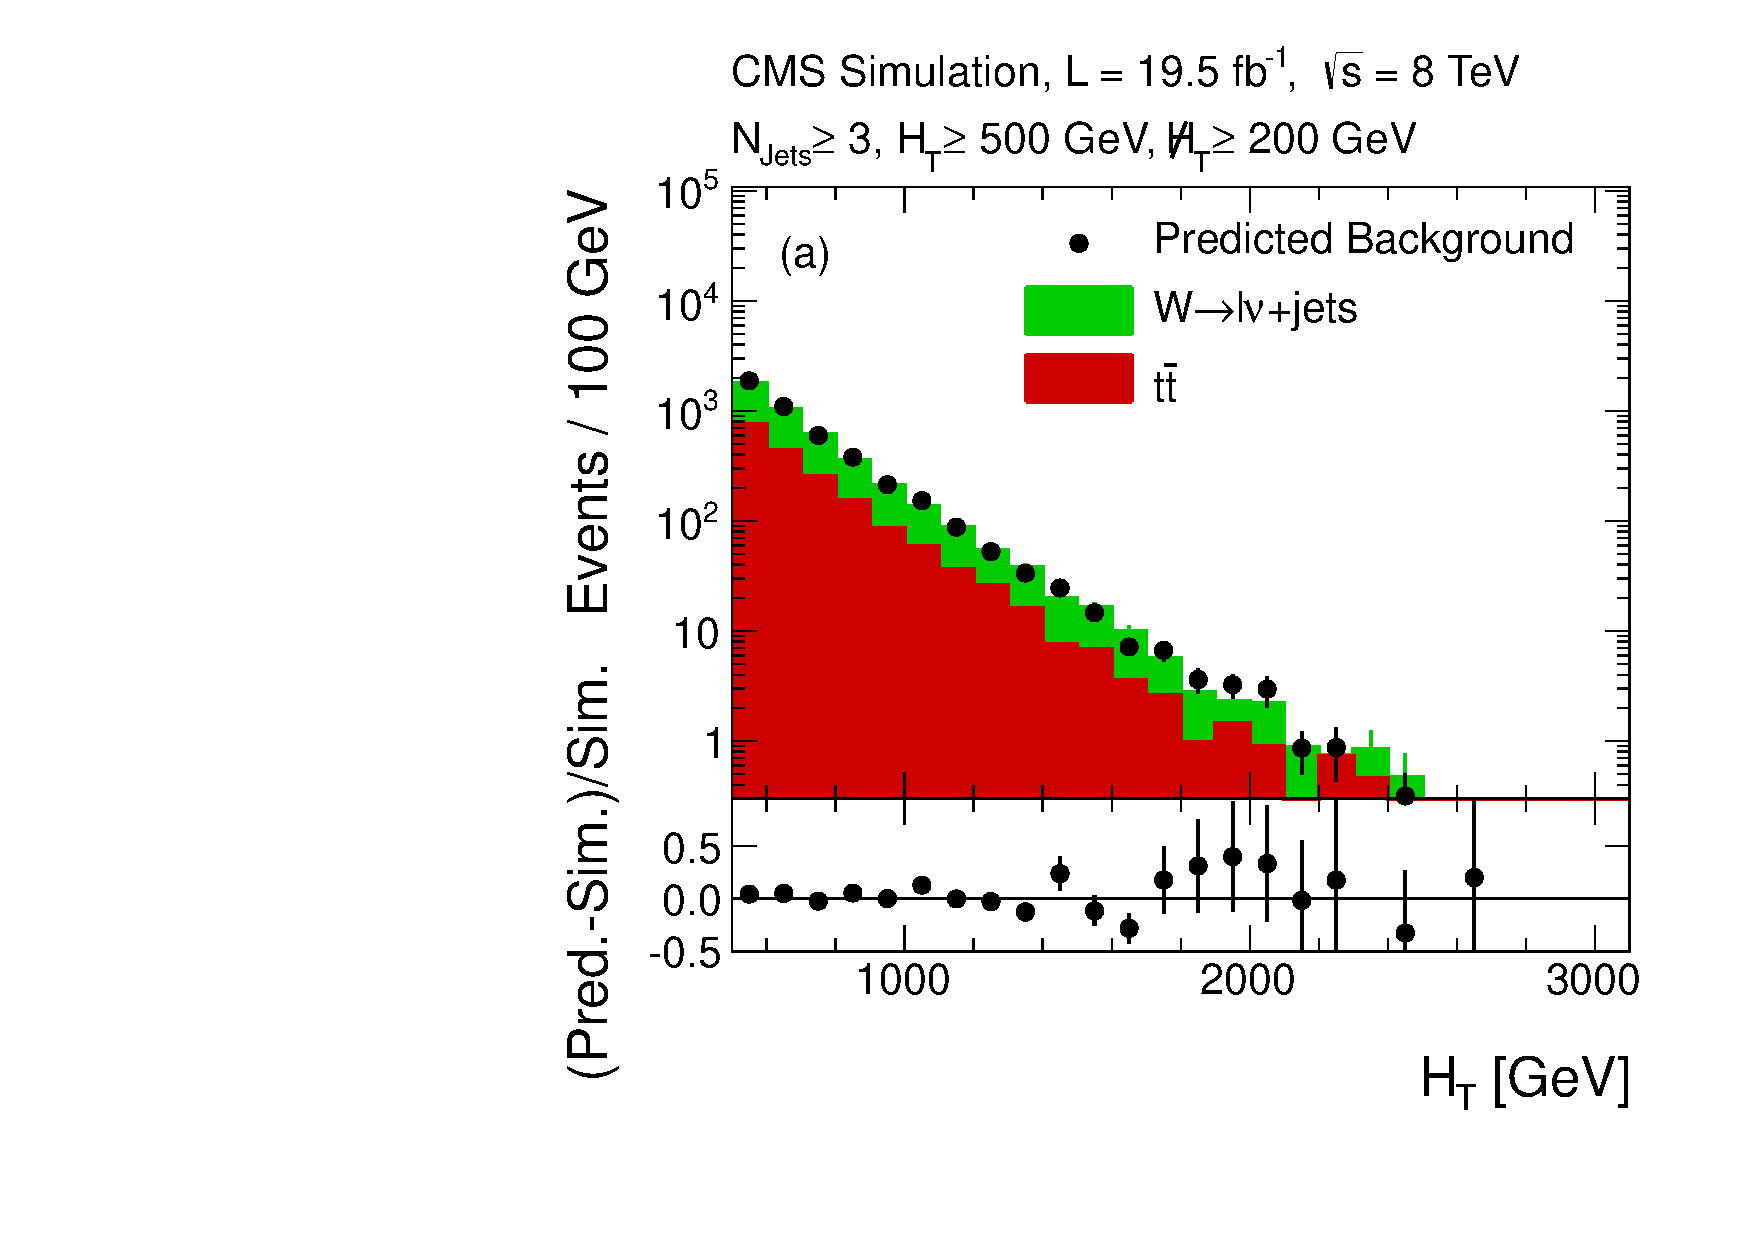
\includegraphics[width=0.49\textwidth]{figures/RA2_LL1.pdf}% \hspace {1.5 pt} 
      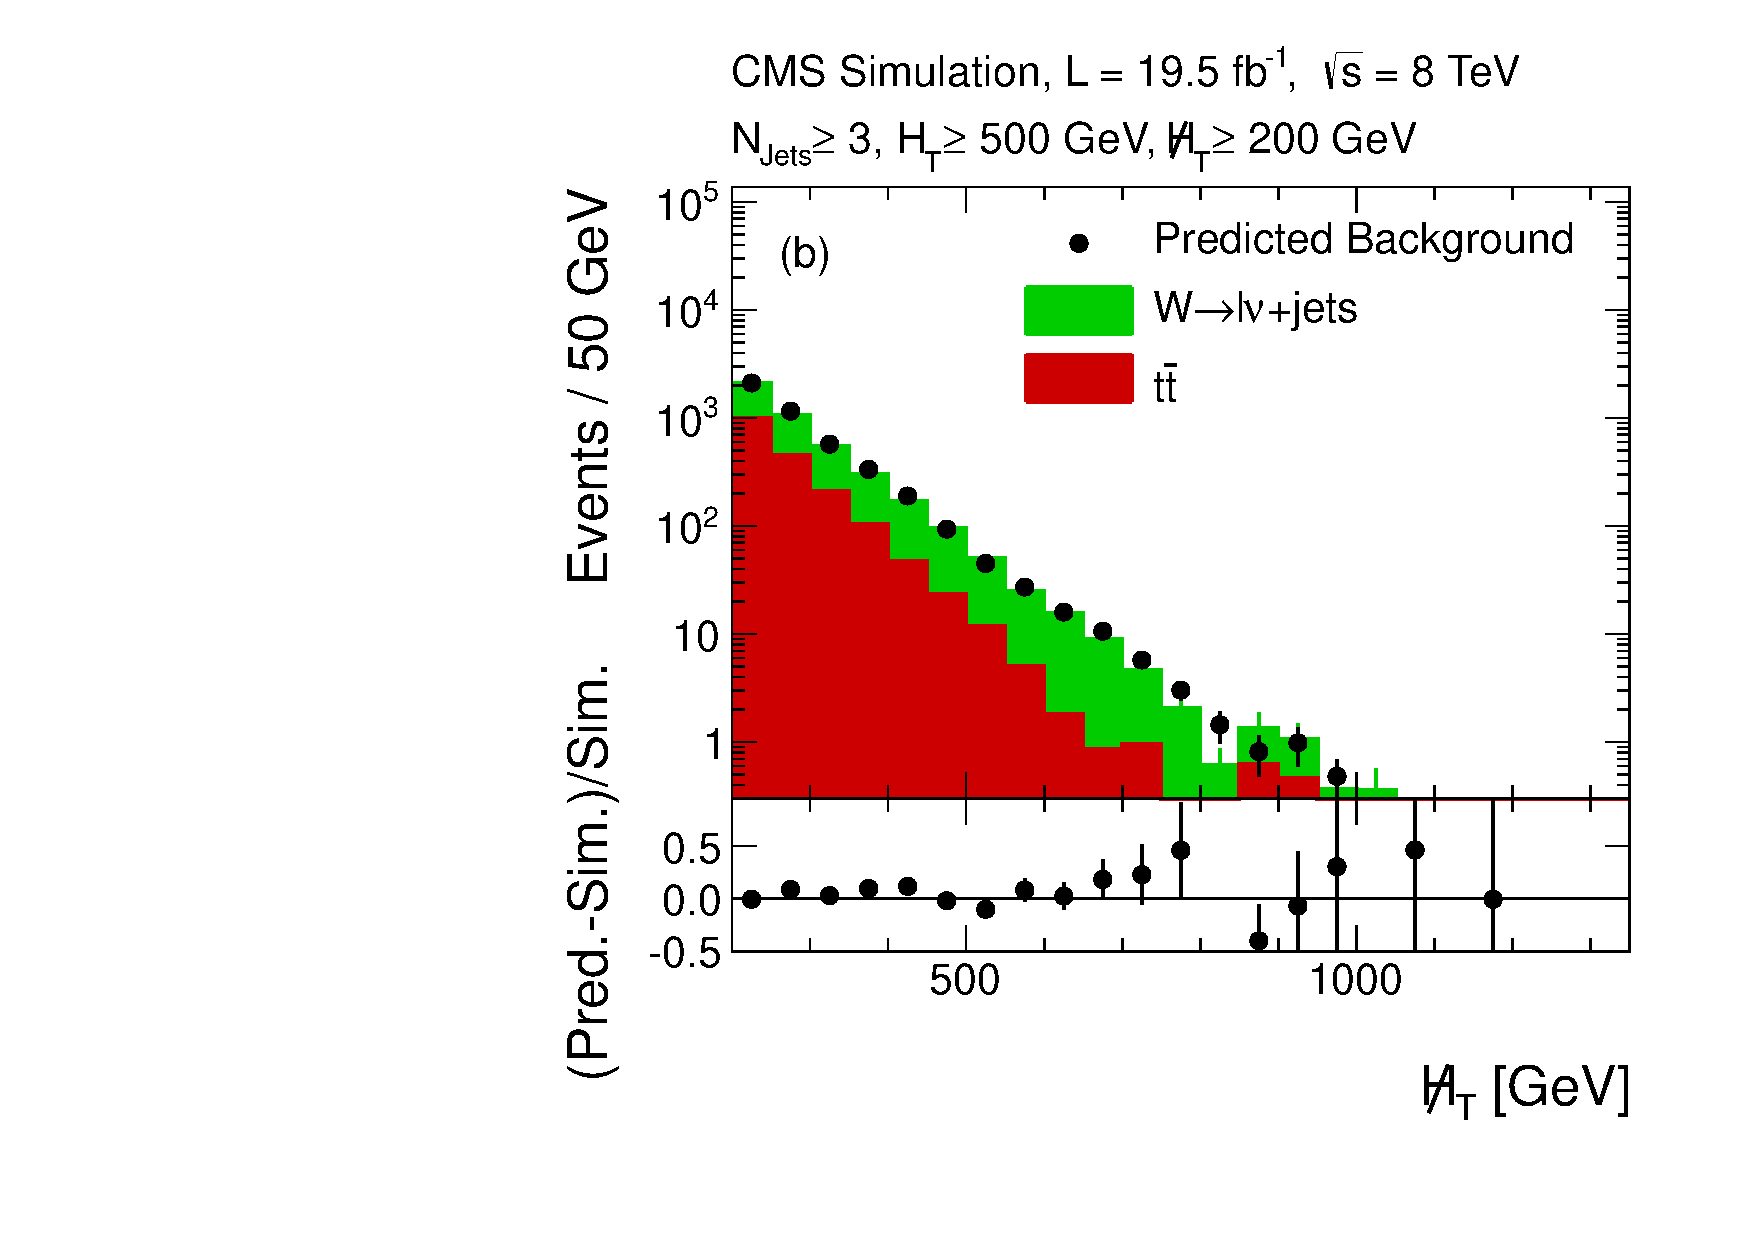
\includegraphics[width=0.49\textwidth]{figures/RA2_LL2.pdf}\\ 
      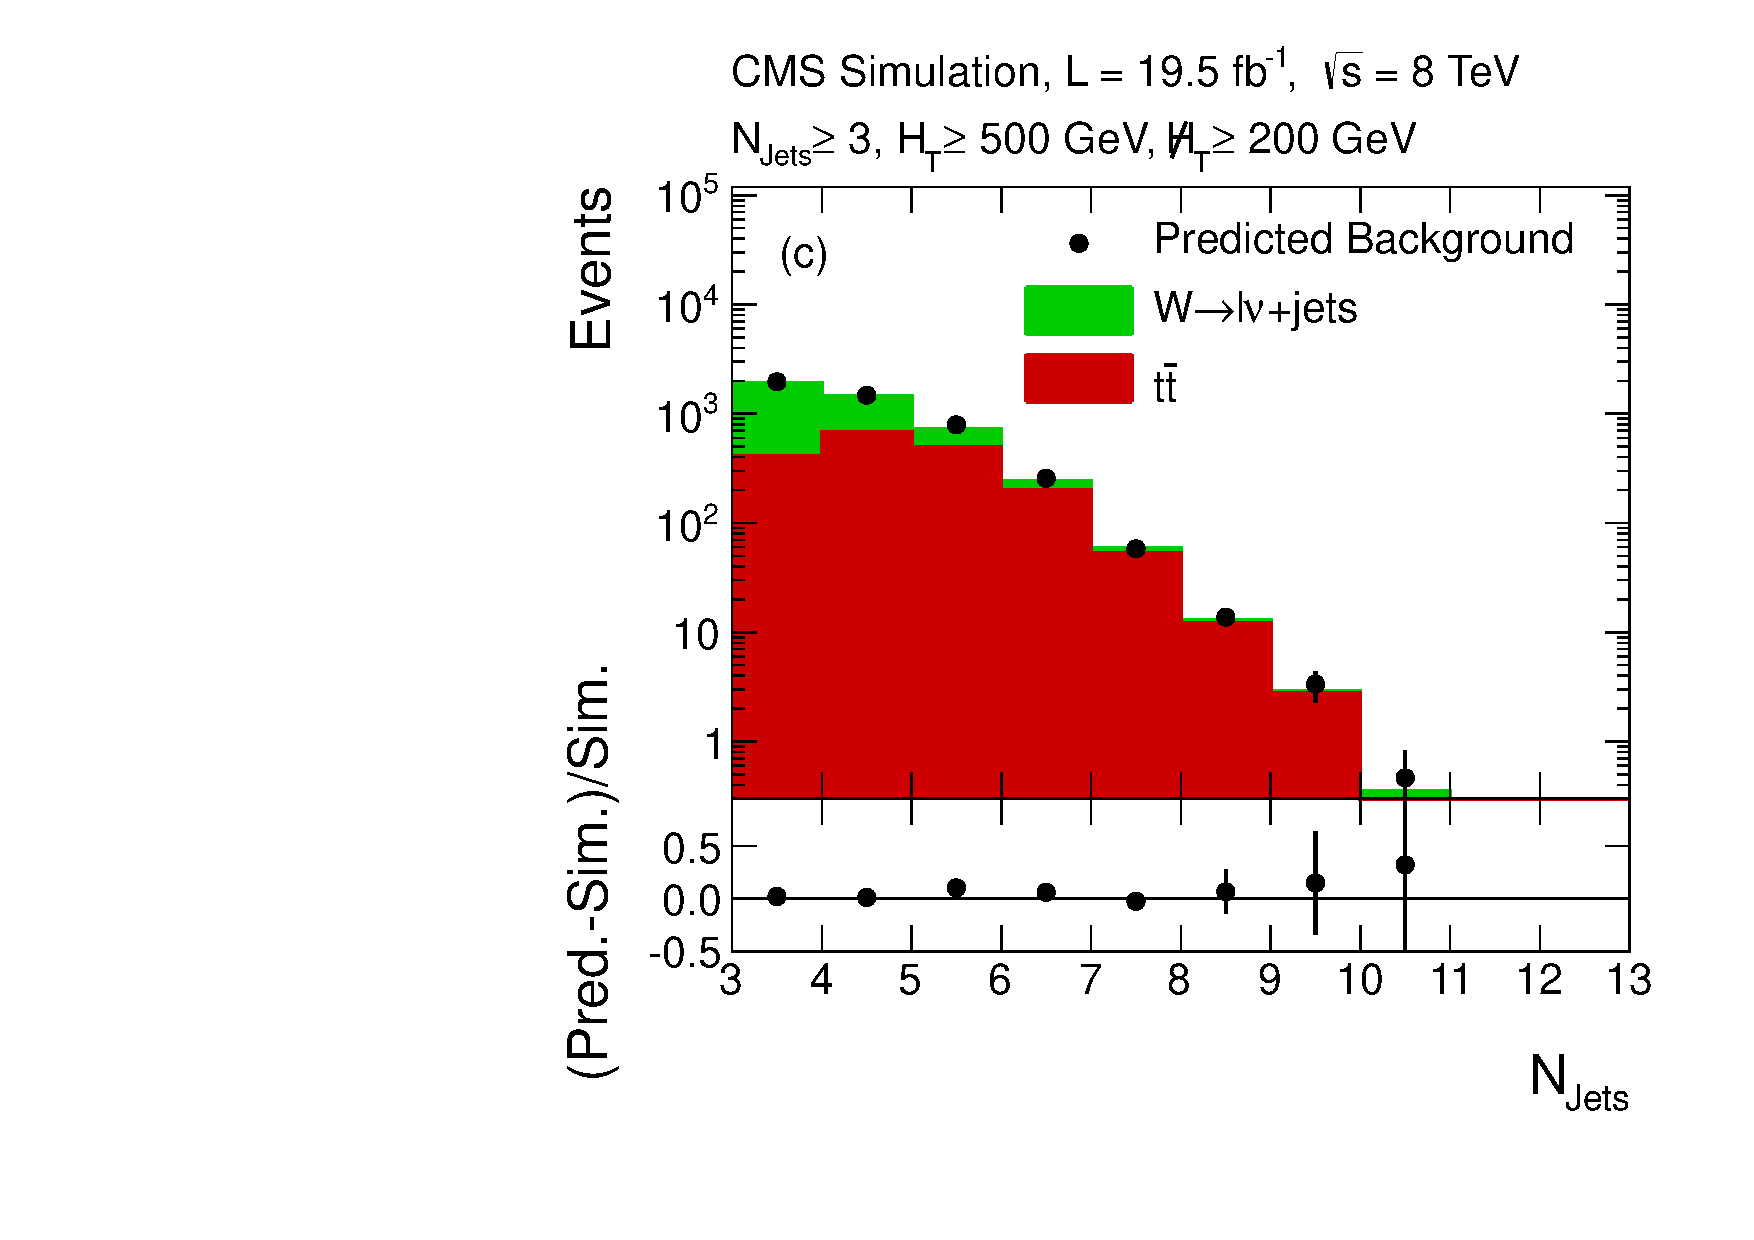
\includegraphics[width=0.49\textwidth]{figures/RA2_LL3.pdf}
    \end{center}
  \end{minipage}

  \caption{Predicted (a) \HT, (b) \MHT, and (c) \NJets distributions found from applying the lost lepton background evaluation method to simulated \ttbar and \WJets events (solid points) in comparison to the genuine \ttbar and \WJets background from simulation (shaded curves). Only statistical uncertainties are shown~\cite{Chatrchyan:2014lfa}.}
  \label{fig:ra2_ll}
\end{figure}
Similarly to background events from hadronic-tau decays, the background contribution due to a failed veto of a light lepton is estimated from a $\mu + \mathrm{jets}$ control sample. This is selected with the same trigger as used as signal trigger for the search. The sample is selected by requiring exactly one well-reconstructed and isolated muon with $\pt > 10$\gev. Furthermore, the same transverse mass requirement of $m_\mathrm{T} < 100$\gev, as for the hadronic tau background, is applied. \\
The number of events in the zero-lepton search regions can be estimated from the single-muon sample by weighting the events according to the lepton reconstruction $\epsilon_\mathrm{reco}^{e, \mu}$ and isolation $\epsilon_\mathrm{iso}^{e, \mu}$ inefficiencies as well as the detector and kinematic acceptance of the muons. The respective efficiencies and acceptances are obtained from simulated \ttbar and \WJets events and determined in intervals of \HT, \MHT and \NJets. \\
The number of events due to unidentified leptons is determined by weighting the events in the control sample according to
\begin{equation*}
\frac{1}{\epsilon_\mathrm{iso}^\mathrm{\mu}} \times \frac{1-\epsilon_\mathrm{reco}^{e, \mu}}{\epsilon_\mathrm{reco}^{\mu}} \; .
\end{equation*}
To account for non-isolated leptons, events in the control sample are weighted with
\begin{equation*}
\frac{\epsilon_\mathrm{reco}^{e, \mu}}{\epsilon_\mathrm{reco}^{\mu}} \times \frac{1-\epsilon_\mathrm{iso}^{e, \mu}}{\epsilon_\mathrm{iso}^{\mu}} \; .
\end{equation*}
\\
The method is validated in simulation by comparing the predicted event yields for lost-lepton events in \ttbar and \WJets from a single-muon control sample after the baseline selection to the simulated genuine background. This comparison is illustrated in Fig.~\ref{fig:ra2_ll} as a function of \HT, \MHT and \NJets and shows a good overall agreement. An uncertainty of 15\% is assigned to jet multiplicities 3--5 and 40\% to other jet multiplicity selections, in order to account for the statistical precision of this validation test.\\
Other uncertainties of the lost-lepton background prediction arise from a lack of events in the control sample in some search regions, differences in lepton reconstruction and isolation efficiency between data and simulation, impact on the acceptance when varying the used PDFs and the acceptance of the transverse mass cut.

\section{QCD Background Estimation with the Rebalance-And-Smear Method}
\label{subsec:RA2_QCD}
The background contribution which is most difficult to model in all-hadronic SUSY searches, is typically QCD background. This is caused by the fact that a precise description of the underlying particle-level jet spectrum and its manifestation in the detector is needed. Especially the former suffers from large theoretical uncertainties, in particular in the extreme kinematic phase space the analysis is performed in. To overcome this, the data-based \textit{Rebalance-and-Smear} (R+S) method was developed. It is based on the assumption that if the momenta of particle-level jets in an event are known, the reconstructed jet momenta can be modelled by a per-jet resolution function. This approach has been successfully used already in previous analyses~\cite{springerlink:10.1007/JHEP08(2011)155, Chatrchyan:2012lia}. In this thesis, essentially improvements of the R+S method are discussed that became necessary to handle the main changes of this analysis when extending the search regions in several jet mulitplicity intervals at $\sqrt{s} = 8$\tev. \\
After the discussion of the general concept of the R+S method in Sec.~\ref{subsec:RPlusS_concept}, the adjustment of the procedure to the actual conditions for 8\tev data are introduced in Sec.~\ref{subsec:RPlusS_app}. This is followed by a description of the validation procedure of the method in Sec.~\ref{subsec:validation_mc}. Furthermore, the application of the R+S method to data is introduced in Sec.~\ref{subsec:validation_data_R+S} and systematic uncertainties are discussed in Sec.~\ref{subsec:RA2_syst_unc}. This section concludes with a presentation of the results of the QCD background prediction in Sec.~\ref{subsec:RA2_qcd_pred}. 

\subsection{General concept of the Rebalance-and-Smear method}
\label{subsec:RPlusS_concept} 
In general, QCD background contributions arise from jet mismeasurements in the detector. The main contributions stem from QCD multijet events which have in principle no intrinsic missing energy, except for neutrinos in jets arising for instance from electroweak decays of heavy-flavour quarks. Minor contributions originate also from fully-hadronic decaying \ttbar, \WJets and \ZJets events. Since QCD background is caused by jet mismeasurements, the general idea is to estimate this background contribution by emulating the measurement of multijet events. \\
In order to do this, the prediction of the QCD background is performed in two subsequent steps. First, the events are \textit{rebalanced}, as described below, such that the missing energy in the event is removed and idealised multijet events denoted \textit{seed events} are obtained. These seed events are estimators of the true particle-level jet momenta. In a second step, all jets in the event are \textit{smeared} with the full jet response function to model the interaction of the multijet state with the detector. This means that all jet momenta are scaled with a factor randomly drawn according to the jet response distribution. Smeared events contain the whole information about event kinematics of the studied background contribution, such that these can be used to derive contributions to various kinematic distributions, like \HT or \MHT. This is a main advantage of the R+S method compared to other QCD background estimation methods which typically predict event rates rather than event kinematics. The general outline of the R+S method is illustrated in Fig.~\ref{fig:RPlusS_concept}.
\begin{figure}[!t]
  \centering
  \makebox[\linewidth]{
  \begin{tabular}{c}
                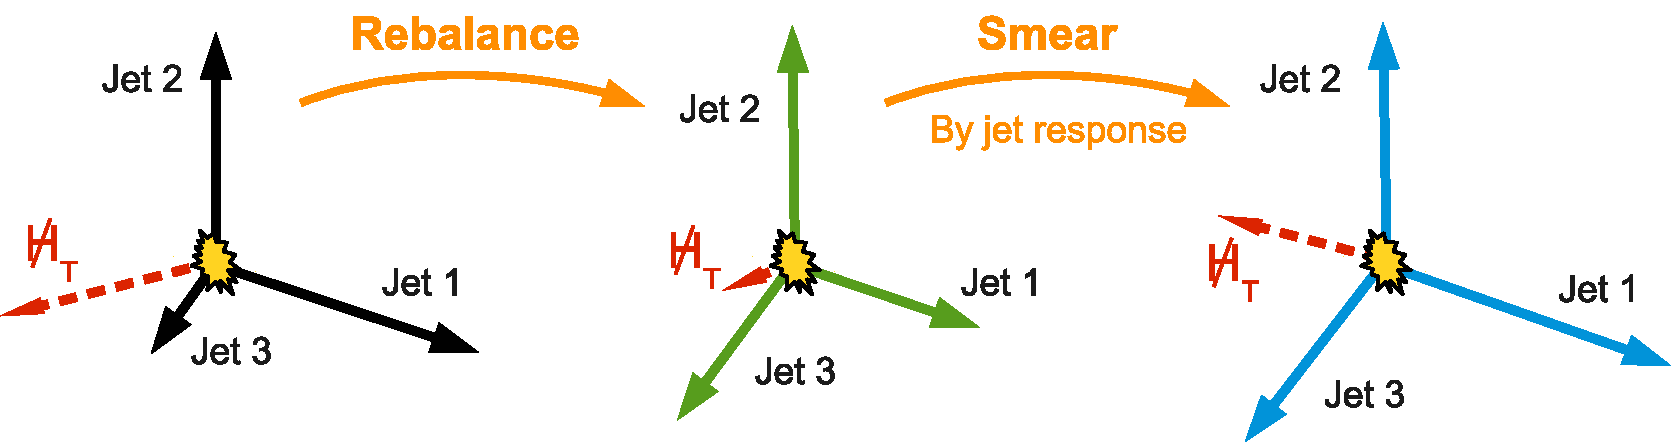
\includegraphics[width=0.99\textwidth]{figures/SketchJetSmearingMethod_LabelMHT.pdf}  
  \end{tabular}}
  \caption{Outline of the two steps performed in the R+S method for estimation of QCD background events. Sketch from~\cite{thesis:Schroeder}.}
  \label{fig:RPlusS_concept}
\end{figure}

 \subsubsection*{Response Templates}
\label{subsubsec:qcd_response}
As indicated above, the R+S method relies on a precise parametrization of the jet response to both perform the rebalancing and the jet smearing. The MC-truth response is derived for simulated QCD multijet events, including the full detector simulation, in intervals of $\pt^\mathrm{gen}$ and $|\eta^\mathrm{gen}|$ as summarized in Tab.~\ref{tab:RPlusS_binning}. Reconstructed jets at detector-level are particle-flow jets clustered with the anti-$k_\mathrm{T}$ algorithm using a distance parameter of $R = 0.5$ including charged-hadron subtraction. These jets are calibrated according to the description in Sec.~\ref{subsec:jets_calib}. Furthermore, the pileup scenario of the simulated sample is reweighted to match the one observed in data, as explained in Sec.~\ref{subsec:jer_sel_cuts}. Although a fine $\pt^\mathrm{gen}$ and $|\eta^\mathrm{gen}|$ binning is chosen, the response is averaged over a certain part of the $\pt^\mathrm{gen}$ spectrum in each interval. Thus, the response distribution tends to overestimate the width of the resolution for high-\pt jets while it behaves oppositely for low-\pt jets. \\
The truth jet response is derived by performing an unambigous one-to-one matching of reconstructed jet $i$ to generated jet $i$ using a distance criterion of $\Delta R < 0.1$. In order to avoid tails from splitting and merging effects of the jet reconstruction, any further reconstructed or generated jet $j \ne i$ around a matched jet pair is vetoed in a cone of size $R < 0.7$ by requiring
\begin{equation}
 \pt^{\rm{GenJet}_j} / \pt^{\rm{GenJet}_i} < 0.05
\end{equation} 
and
\begin{equation}
 \pt^{\rm{Jet}_j} < 30\,\mathrm{GeV} \;\; \mathrm{and} \;\; \pt^{\rm{Jet}_j} / \pt^{\rm{Jet}_i} < 0.05 \; .
\end{equation} 
The obtained jet response distributions are averaged over all jets in an event not separating them according to their rank, \ie their position in a descending \pt order, or according to the jet flavour. Thus, they reflect the flavour composition of an average QCD multijet sample. One example response distribution is illustrated in Fig.~\ref{fig:RPlusS_response}. Here, the blue line indicates the response as used in the R+S method, while the red line shows the response distribution for b jets. The latter illustrates that the lower tail of the response is mainly due to the decay of heavy-flavour quarks.
\begin{table}[!t]
\centering
\caption{Overview of the $|\eta^\mathrm{gen}|$ and $\pt^\mathrm{gen}$ interval boundaries used for the MC-truth response determination used as input for the R+S method.}
\label{tab:RPlusS_binning}
\makebox[\linewidth]{
\begin{tabular}{c}
\multicolumn{1}{c}{} \\
\toprule
 $|\eta^\mathrm{gen}|$ \\
 0, 0.3, 0.5, 0.8, 1.1, 1.4, 1.7, 2.0, 2.3, 2.8, 3.2, 4.1, 5.0 \\
\midrule
$\pt^\mathrm{gen} \; [\mathrm{GeV}]$ \\
0, 20, 30, 50, 80, 120, 170, 230, 300, 380, \\
470, 570, 680, 800, 1000, 1300, 1700, 2200, 2800, 3500 \\
\bottomrule
\end{tabular}}
\end{table} 
\\
The truth response templates to be used for applying the R+S method in simulated events, \eg for validation tests, are determined as described above. However, when using the truth response templates for the actual QCD background predictions in data, they have to be corrected for potential data-to-simulation jet resolution differences. As seen in Chap.~\ref{chap:Resolution}, the resolution in data is typically worse than in simulation. Thus, the determined truth response templates are adjusted accordingly. This correction is done for the Gaussian core and the non-Gaussian tails separately. For that purpose, the response function is splitted into the respective core and tail parts. This is done by fitting the response distribution with a Gaussian in the range of $\pm$ 1\,RMS around the mean which is then subtracted from the total response distribution in order to obtain the tail parts. The correction factors for the core resolution are applied by convoluting the MC-truth response with a Gaussian of width $\sigma_{c}$ according to Eq.~\ref{eq:res_adjust}. The considered correction factors are listed in Tab.~\ref{tab:jer_RPlusS_core} in the appendix and correspond to the data-to-simulation ratios obtained from dijet data at $\sqrt{s} = 7$\tev, as illustrated in Fig.~\ref{fig:result_comparison} (right).\footnote{Although the correction factors for the data-to-simulation ratio derived in the context of this thesis are more precise, these have not been available when the analysis presented here has been performed.} The residual tail contributions are scaled according to the correction factors $\rho_\mathrm{tail}$ listed in Tab.~\ref{tab:jer_RPlusS_tails} in the appendix derived from dijet asymmetry parts fulfilling $(\mathrm{A} > 2 \sigma_c)$~\cite{thesis:Schroeder}.   
\begin{figure}[!t]
  \centering
  \makebox[\linewidth]{
  \begin{tabular}{c}
                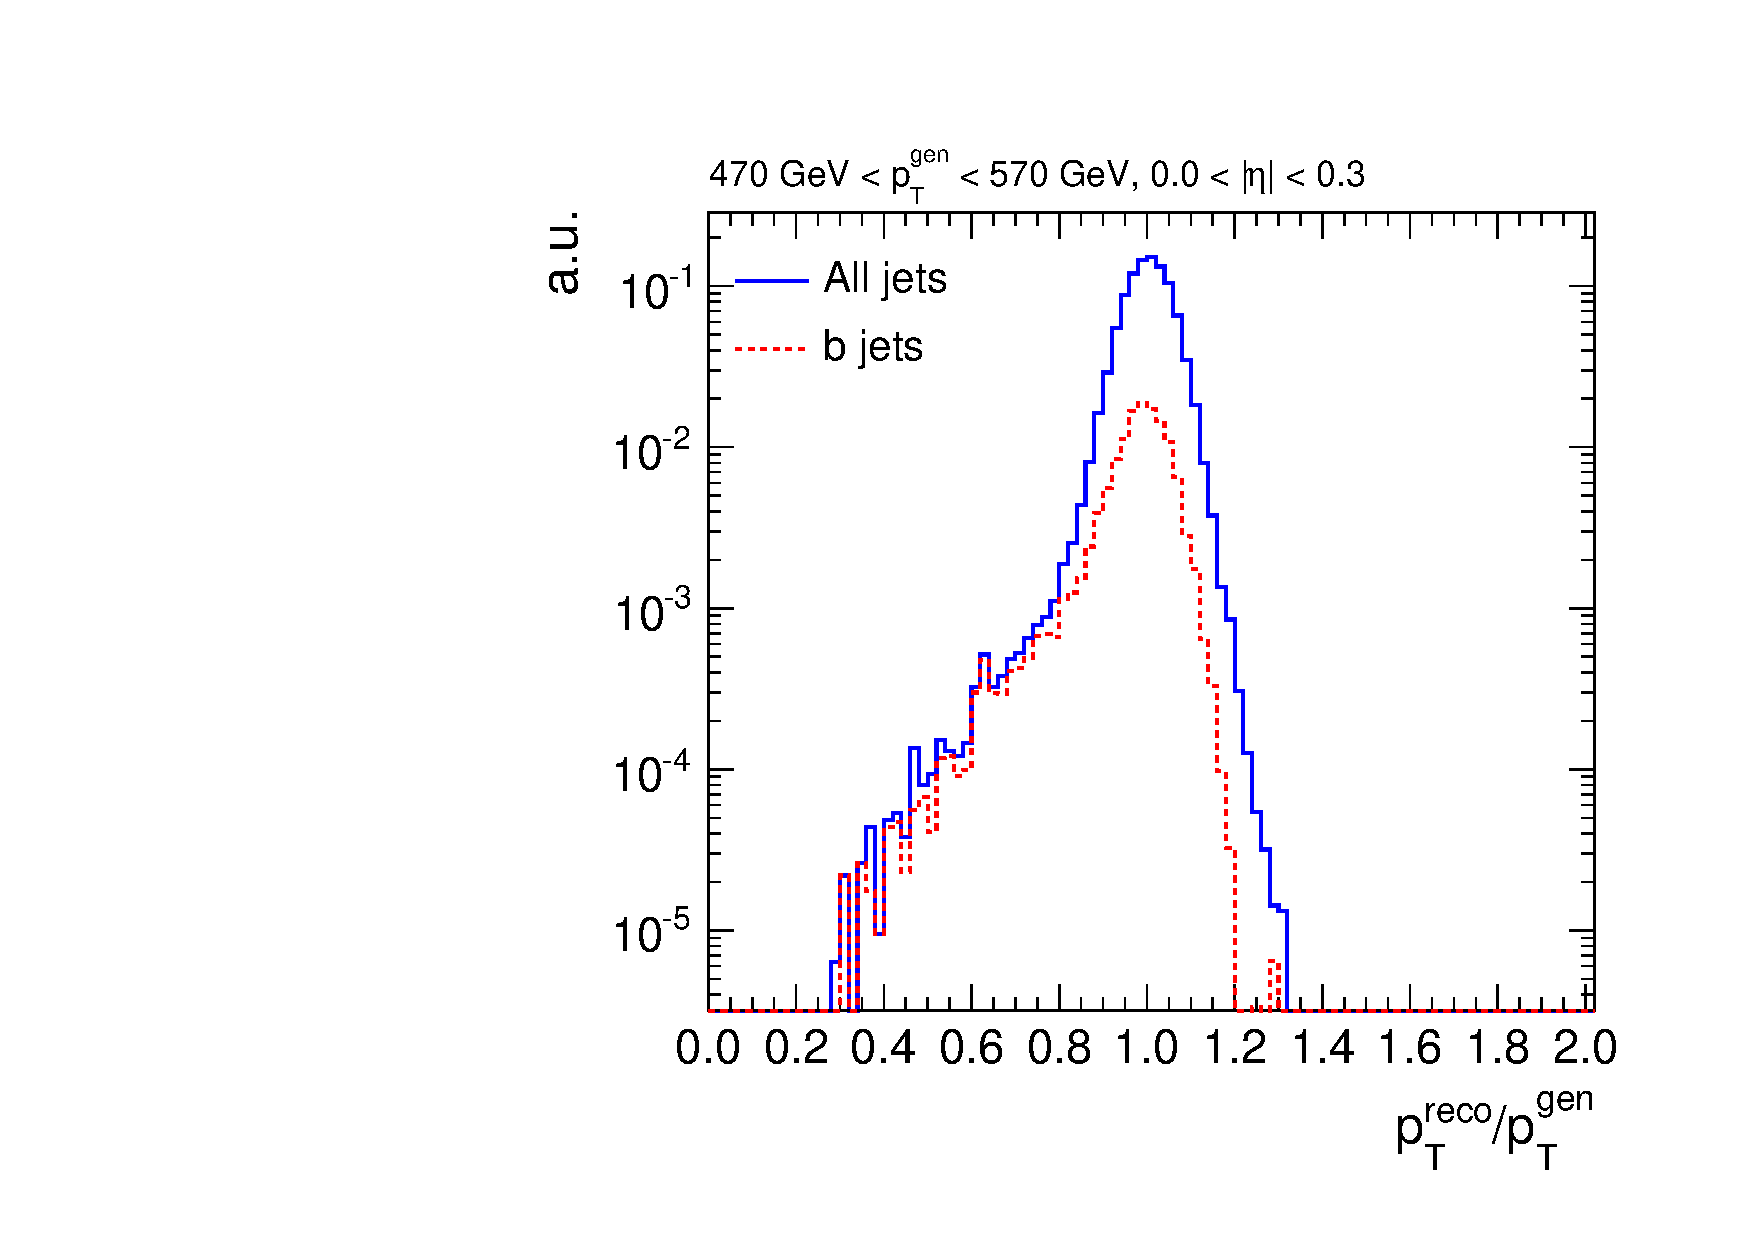
\includegraphics[width=0.49\textwidth]{figures/ResponseTemplate_b_all_pythia.pdf}  
  \end{tabular}}
  \caption{Example truth response template as used in the R+S method for one particular $\pt^\mathrm{gen}$ and $|\eta^\mathrm{gen}|$ interval averaged over all jets (\textit{blue line}) and for b jets only (\textit{red line}).}
  \label{fig:RPlusS_response}
\end{figure}

\subsubsection*{Rebalance Procedure}
\label{subsubsec:qcd_rebalancing}
As stated above, the first step in the R+S method is to create a sample of seed events that serve as estimator of the true particle-level jets by performing a rebalancing of the multijet events. This rebalancing is done based on a \textit{kinematic fit}~\cite{D'Hondt:926540}. \\
This fit is based on the assumption that for a given event, all measured and unmeasured quantities fulfill certain kinematic constraints, like energy and momentum conservation. However, due to the uncertainties of the measured quantities, these constraints are not exactly fulfilled. Thus, the constraints can be used to adjust the measured values within the uncertainties to meet the event hypothesis. This is done on an event-by-event basis by performing a least-square fit considering the kinematic constraints by Lagrange multipliers. These Lagrange multipliers provide a general method to determine local extrema of non-linear functions of many variables. Mathematically, the likelihood function 
\begin{equation}
-2 \; \mathrm{ln}[L(\vec{y}_\mathrm{true})] = d\vec{y}^{\,T} C^{-1} d \vec{y} 
\end{equation}
with $dy^i = y_{\mathrm{true}}^i - y_{\mathrm{measured}}^i$ and covariance matrix $C$ is minimised. In this particular case, the measured jet four-momenta correspond to the values of $y_{\mathrm{measured}}^i$ and are fitted using the constraint of transverse momentum balance. The covariance matrix is given by the jet resolution. However, since the resolution for the angular components is not explicitly determined, in fact no proper angular fit is performed. Thus, the imbalance in each multijet event is removed by actually scaling the jet transverse momenta within the range of the respective resolutions which are approximated by the Gaussian MC-truth resolution. For each response template, the Gaussian core is extracted, as described above, by performing a fit with a Gaussian function within $\pm$ 1\,RMS around the mean. The obtained resolutions with uncertainties from the Gaussian fit are illustrated as a function of $\pt^\mathrm{gen}$ for two example $|\eta^\mathrm{gen}|$ intervals in Fig.~\ref{fig:qcd_rs_truth_res}. Subsequently, the obtained resolution values are fitted with the function
\begin{equation}
\frac{\sigma_\mathrm{MC}(\pt)}{\pt} = \sqrt{\mathrm{sgn}(N) \cdot \left(\frac{N}{\pt}\right)^2 + S^2 \cdot \pt^{m-1} + C^2} \; ,
\end{equation} 
with free parameters $N, S, C$ and $m$. This function is a modified version of Eq.~\ref{eq:NSC} introduced in Chap.~\ref{chap:Resolution} for the characterization of the resolution. It is adjusted here to better describe the resolution of particle-flow jets. The term $\mathrm{sgn}(N)$ considers the improved momentum resolution at low \pt due to the employed tracking information. Since also at medium \pt the tracking information still compensates for non-linearities of the calorimeters, the parameter $m$ is introduced. The fitted functions are illustrated in Fig.~\ref{fig:qcd_rs_truth_res} as red curve and used as input for the kinematic fit. The whole set of truth resolution histograms displayed with the fitted resolution functions for all $|\eta^\mathrm{gen}|$ intervals used as input for the kinematic fit are illustrated in Fig.~\ref{app:fig:qcd_rs_truth_res} and Fig.~\ref{app:fig:qcd_rs_truth_res2} in the appendix. 
\begin{figure}[!t]
  \centering
  \begin{tabular}{cc}
                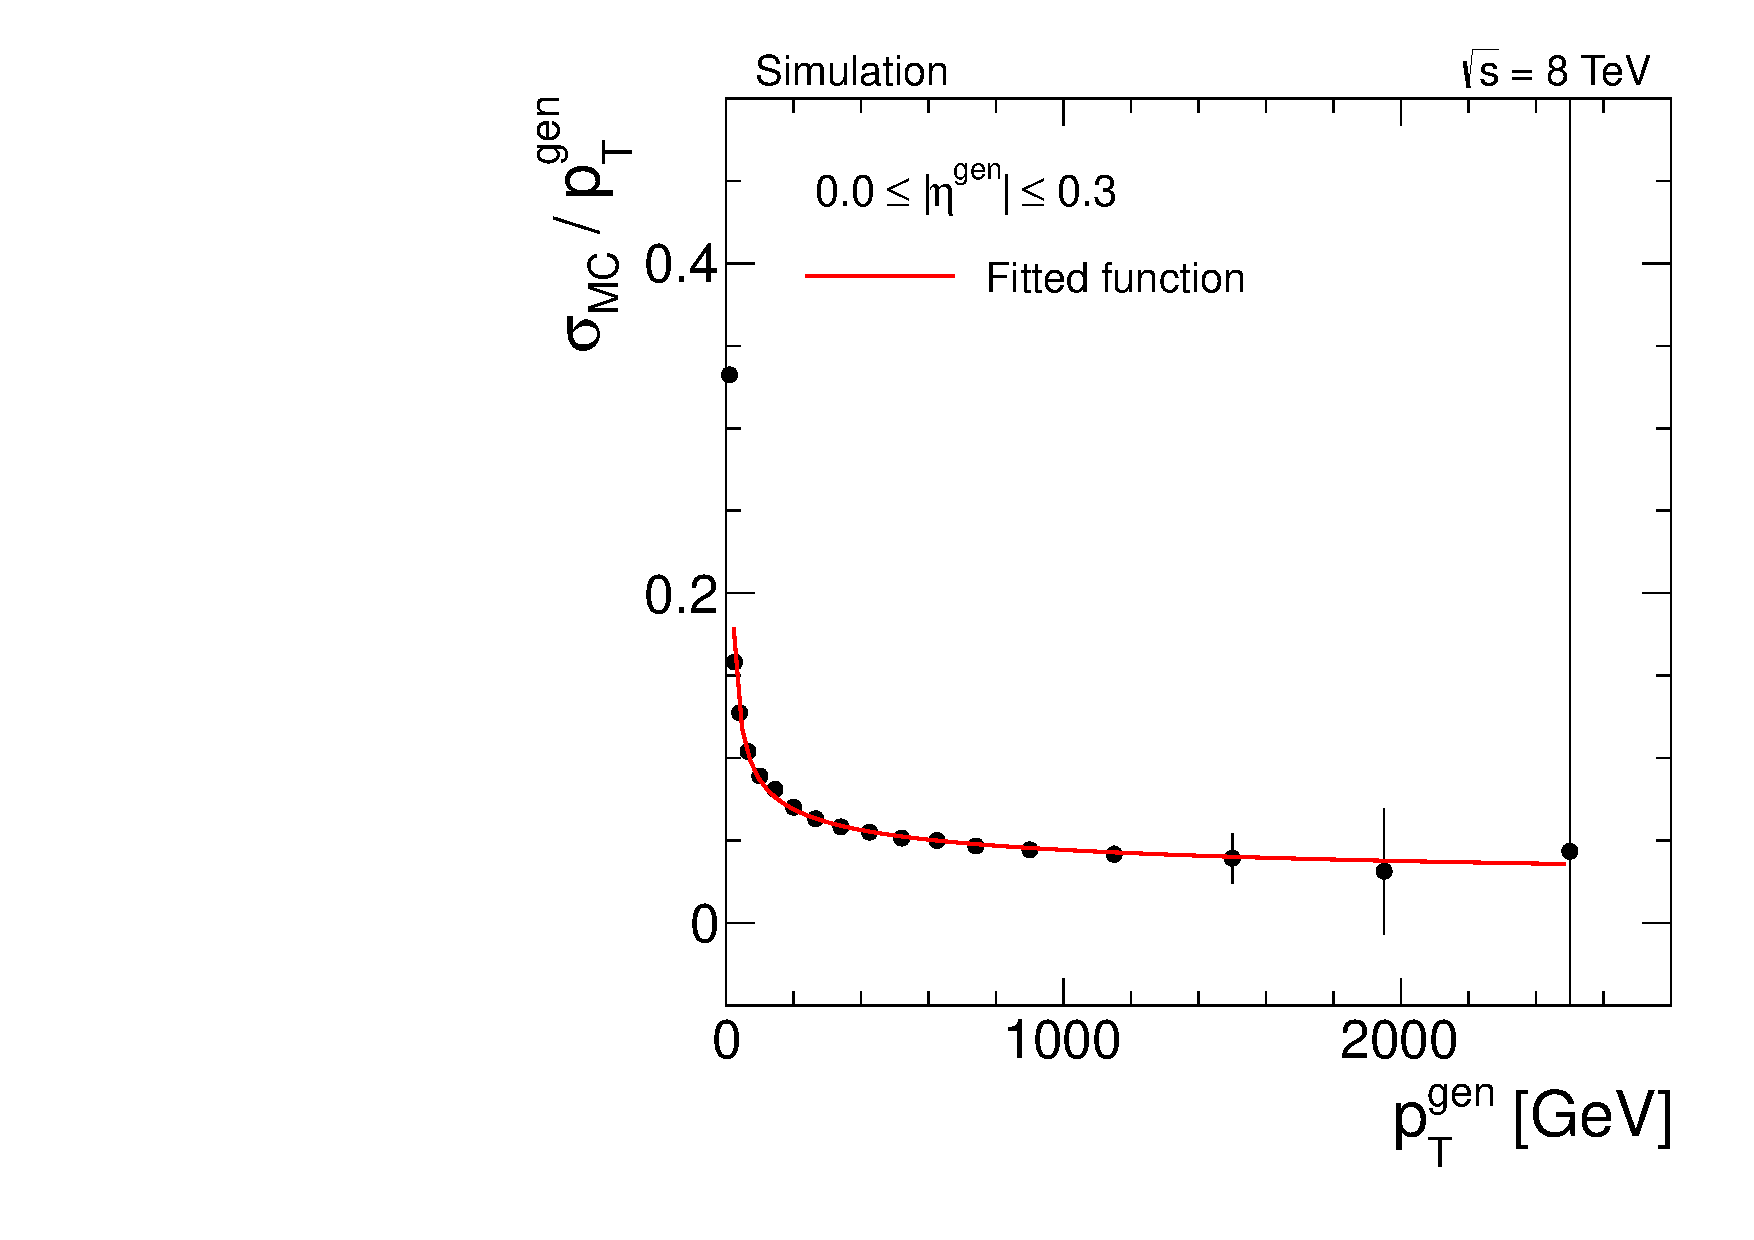
\includegraphics[width=0.49\textwidth]{figures/TruthRes_Eta0.pdf} &
                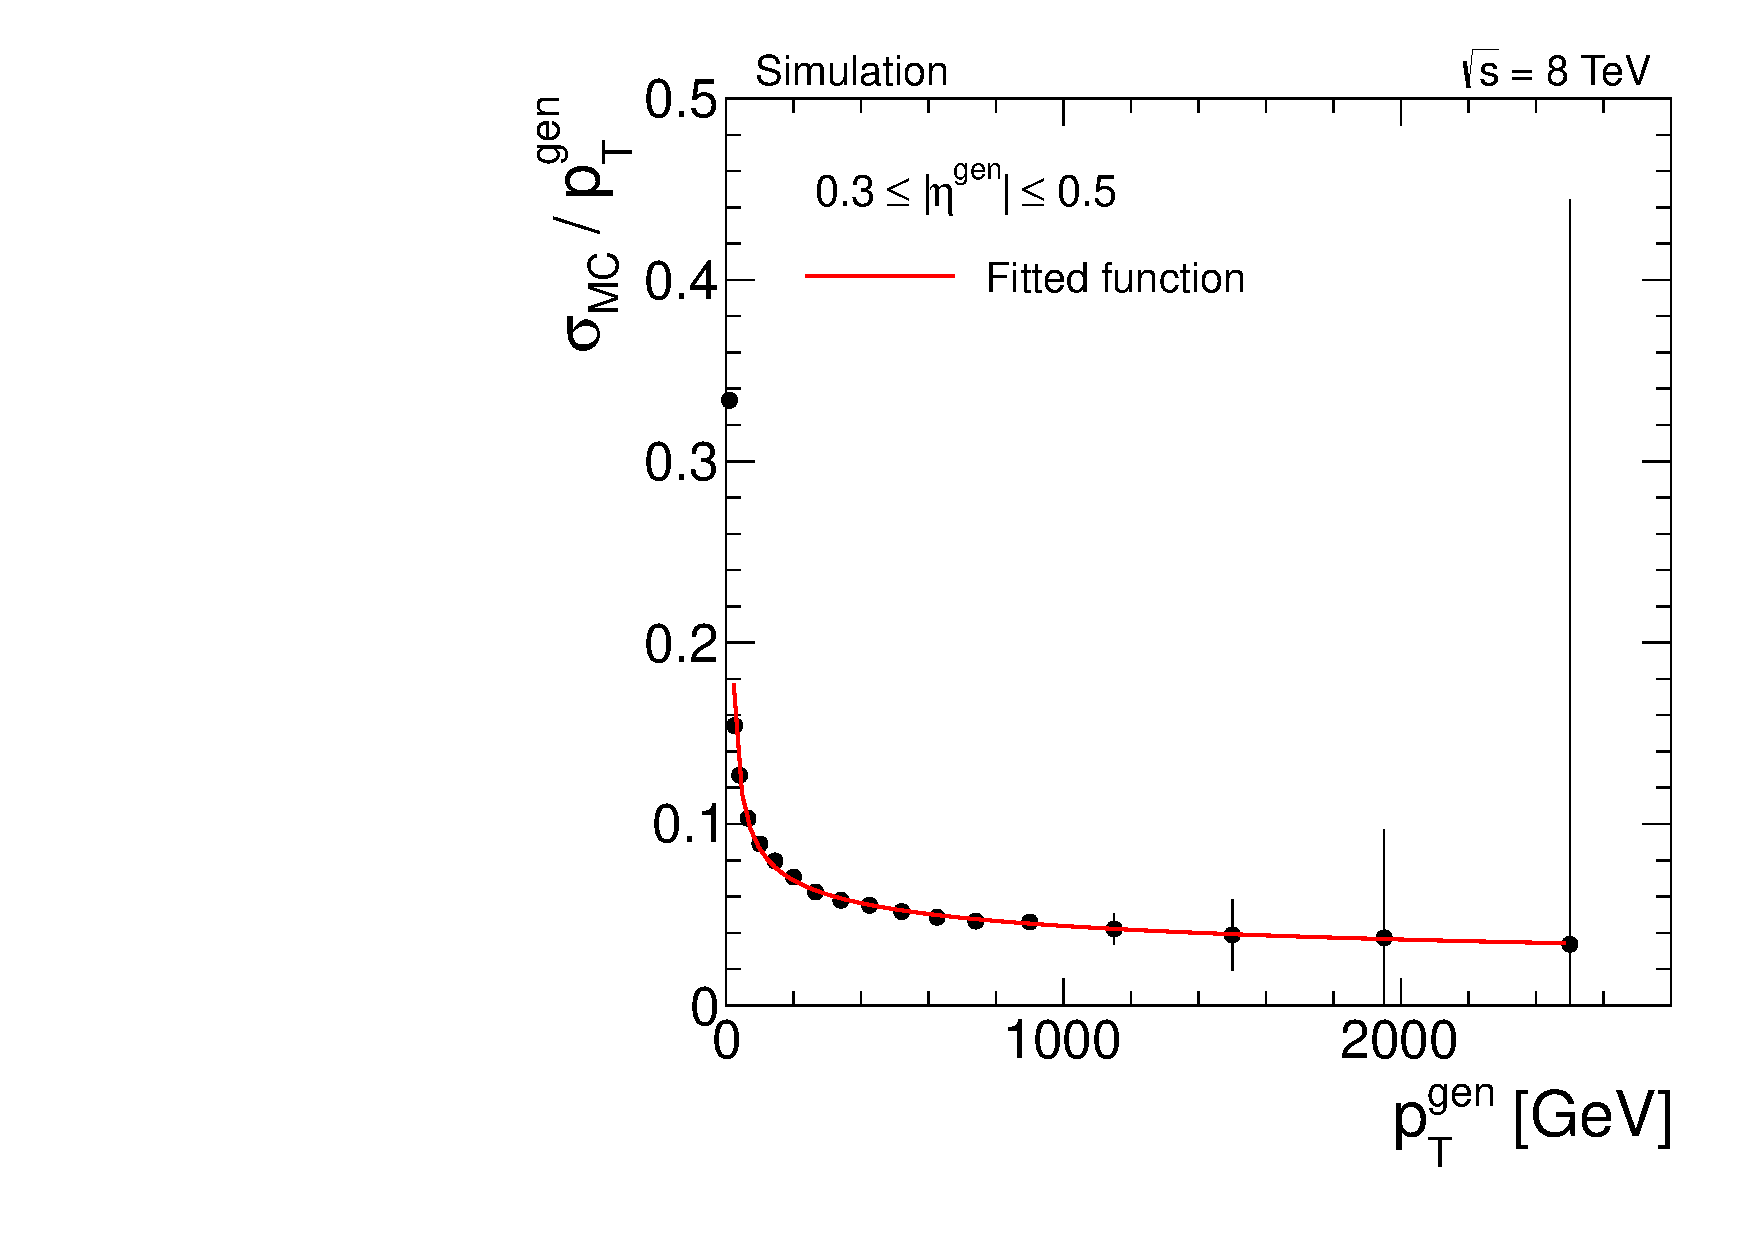
\includegraphics[width=0.49\textwidth]{figures/TruthRes_Eta1.pdf} 
  \end{tabular}
  \caption{Relative truth-\pt resolution derived from simulated events shown as a function of $\pt^\mathrm{gen}$. The distribution is fitted with a function as described in the text used as input for the kinematic fit employed to gain a balanced seed sample.}
  \label{fig:qcd_rs_truth_res}
\end{figure}
\\
Finally, all events for which the fit converged within ($|\MHT^x| + |\MHT^y| < 0.02$\gev) are kept as seed events. Contributions to the seed sample from non-QCD multijet SM processes or even signal events in data do not have to be treated specially. Although these events might get successfully balanced, their contribution to the seed sample is negligible, since their production cross section is orders of magnitudes smaller than the QCD multijet production cross section (\cf Fig.~\ref{fig:CrossSections}). \\
Furthermore, the kinematic fit allows to generate a seed sample from an inclusive sample. This is an advantage compared to for instance defining a seed sample by selecting data events with low values of \MHT, since selections suppressing high tails of missing energy often tend to bias the QCD kinematics. Typically, \HT and \MHT are correlated quantities in QCD events, as high values of \MHT caused by severe jet mismeasurements can only occur, if there is a certain amount of energy in the event. Consequently, selection cuts removing high-\MHT tails also remove parts of the \HT spectrum which results in an overall underestimation of QCD contributions to the high \HT and \MHT tails. Thus, the rebalancing of an inclusive sample with a kinematic fit allows to generate an unbiased seed sample.  

\subsubsection*{Response Smearing}
\label{subsubsec:qcd_smearing}
The second step of the R+S method is the smearing procedure. Here, all jets of a seed event are smeared with the full jet response distributions including non-Gaussian tails. This means that for each event the magnitudes of the transverse momenta of the jets are scaled with a factor that is randomly obtained from the jet response distribution histogram of the respective $\pt$ and $|\eta|$ interval to model the reconstructed transverse momentum. These smeared events hence resemble the full QCD event kinematics and thus contributions from QCD events to the search regions can be estimated by imposing the respective selection cuts to the smeared events. \\
However, this procedure typically results in predictions with large statistical uncertainties, since the probability that a seed event is smeared into the signal region is small. In order to obtain a more robust estimate of the prediction, each event is smeared not only once, but $N = 100$ times (bootstrap method). The mean of these $N$ predictions is considered as final result while the statistical uncertainty is obtained as the standard deviation of the mean estimate, \ie the standard deviation of the set of predictions divided by $1/\sqrt{N}$. This definition of the statistical uncertainty of the prediction ignores the statistical fluctuations of the seed sample. However, since the seed sample is very large, this uncertainty is negligible to good approximation. \\
In order to validate the smearing procedure, generated QCD multijet events obtained from the \madgraph generator are smeared as described above and compared to fully simulated events at reconstruction level. This is performed on a sample with loose pre-selection at detector-level of $\NJets \ge 2$ and $\HT > 350$\gev.\footnote{The same pre-selection is applied to all simulated and data samples studied in this chapter. This does not bias the QCD prediction, since both cut values are sufficiently below the analysis selection criteria.} The result of this generator-jet smearing is shown in Fig.~\ref{fig:qcd_rs_genjets}. 
\begin{figure}[!t]
  \centering

  \begin{minipage}[c]{1.\textwidth}
    \begin{center}
      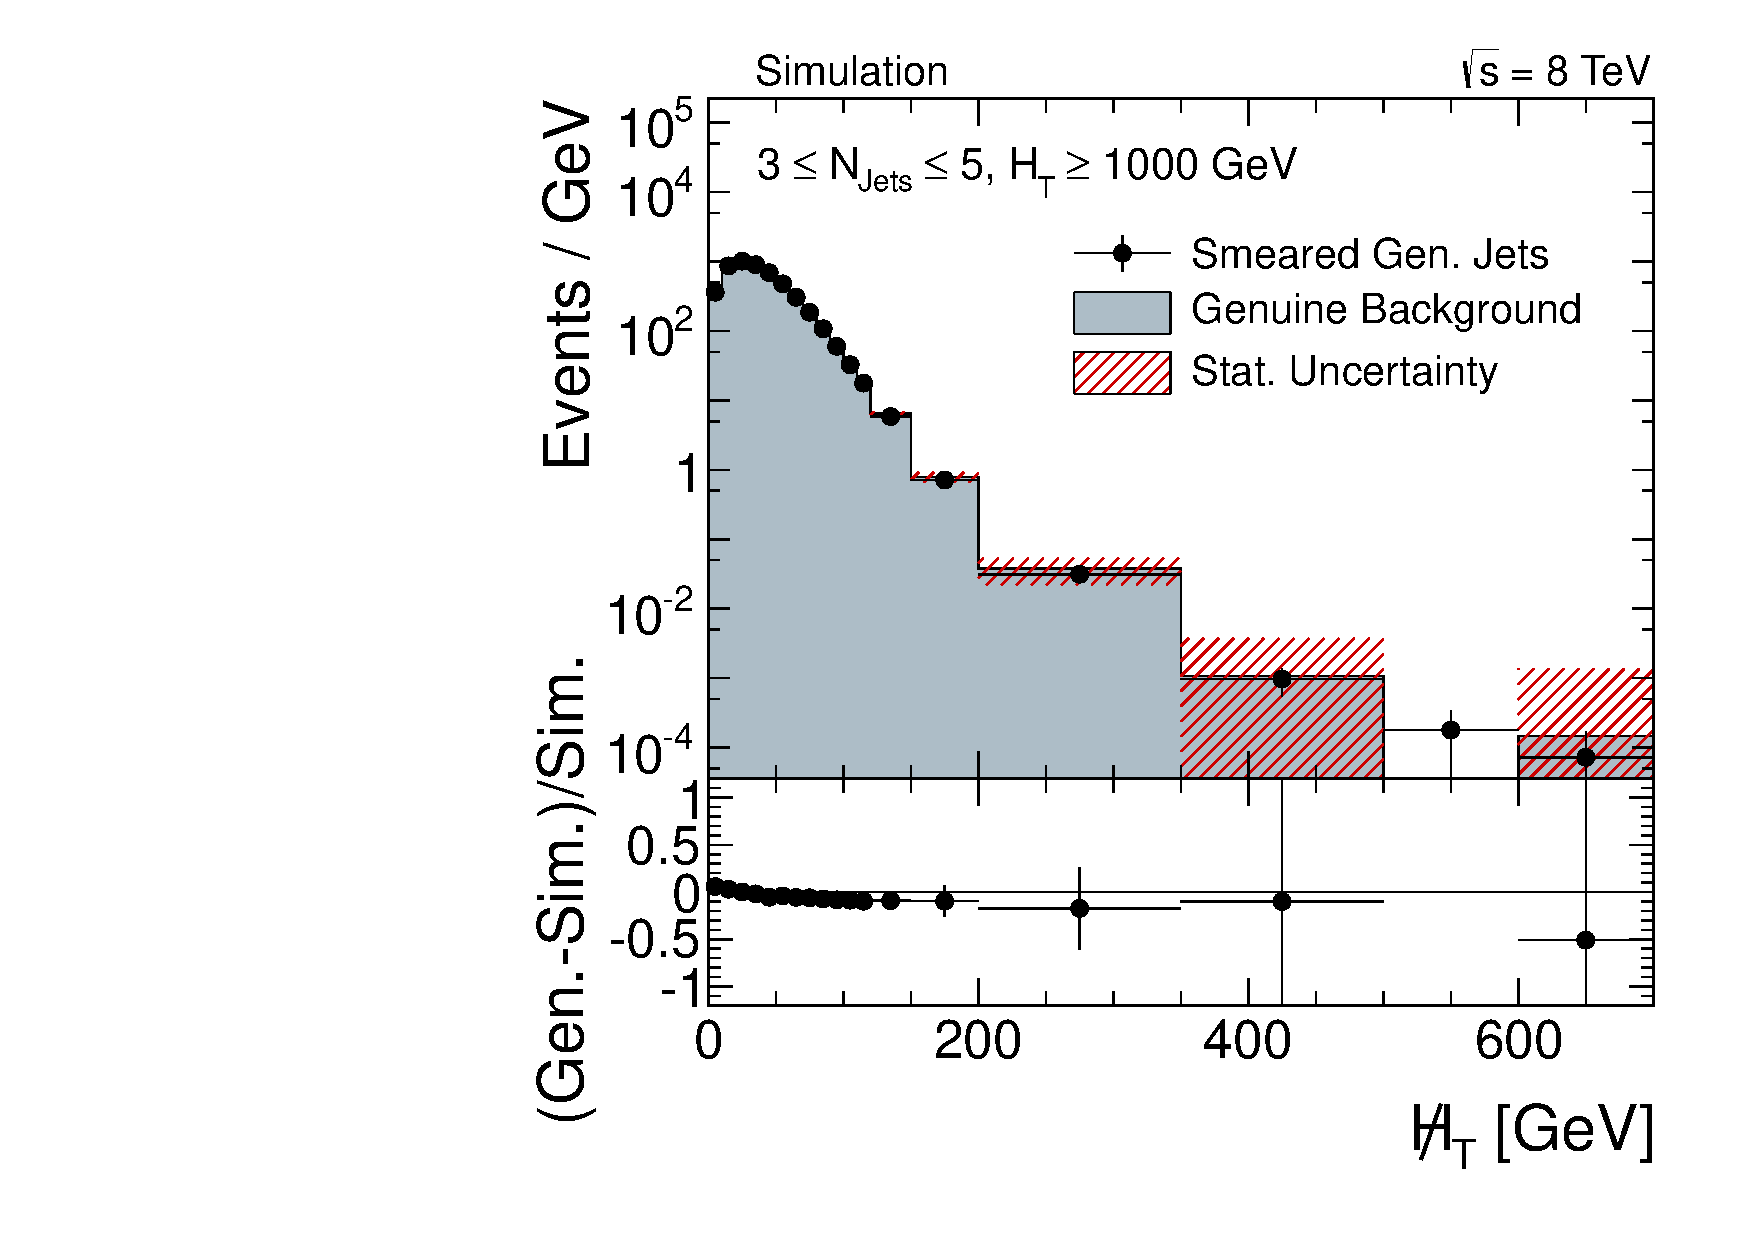
\includegraphics[width=0.49\textwidth]{figures/MHT_JetBin2_HThigh_madgraph_DR53X_chs_withoutPUReweighting_SmearedGenJets_v1.pdf}% \hspace {1.5 pt} 
      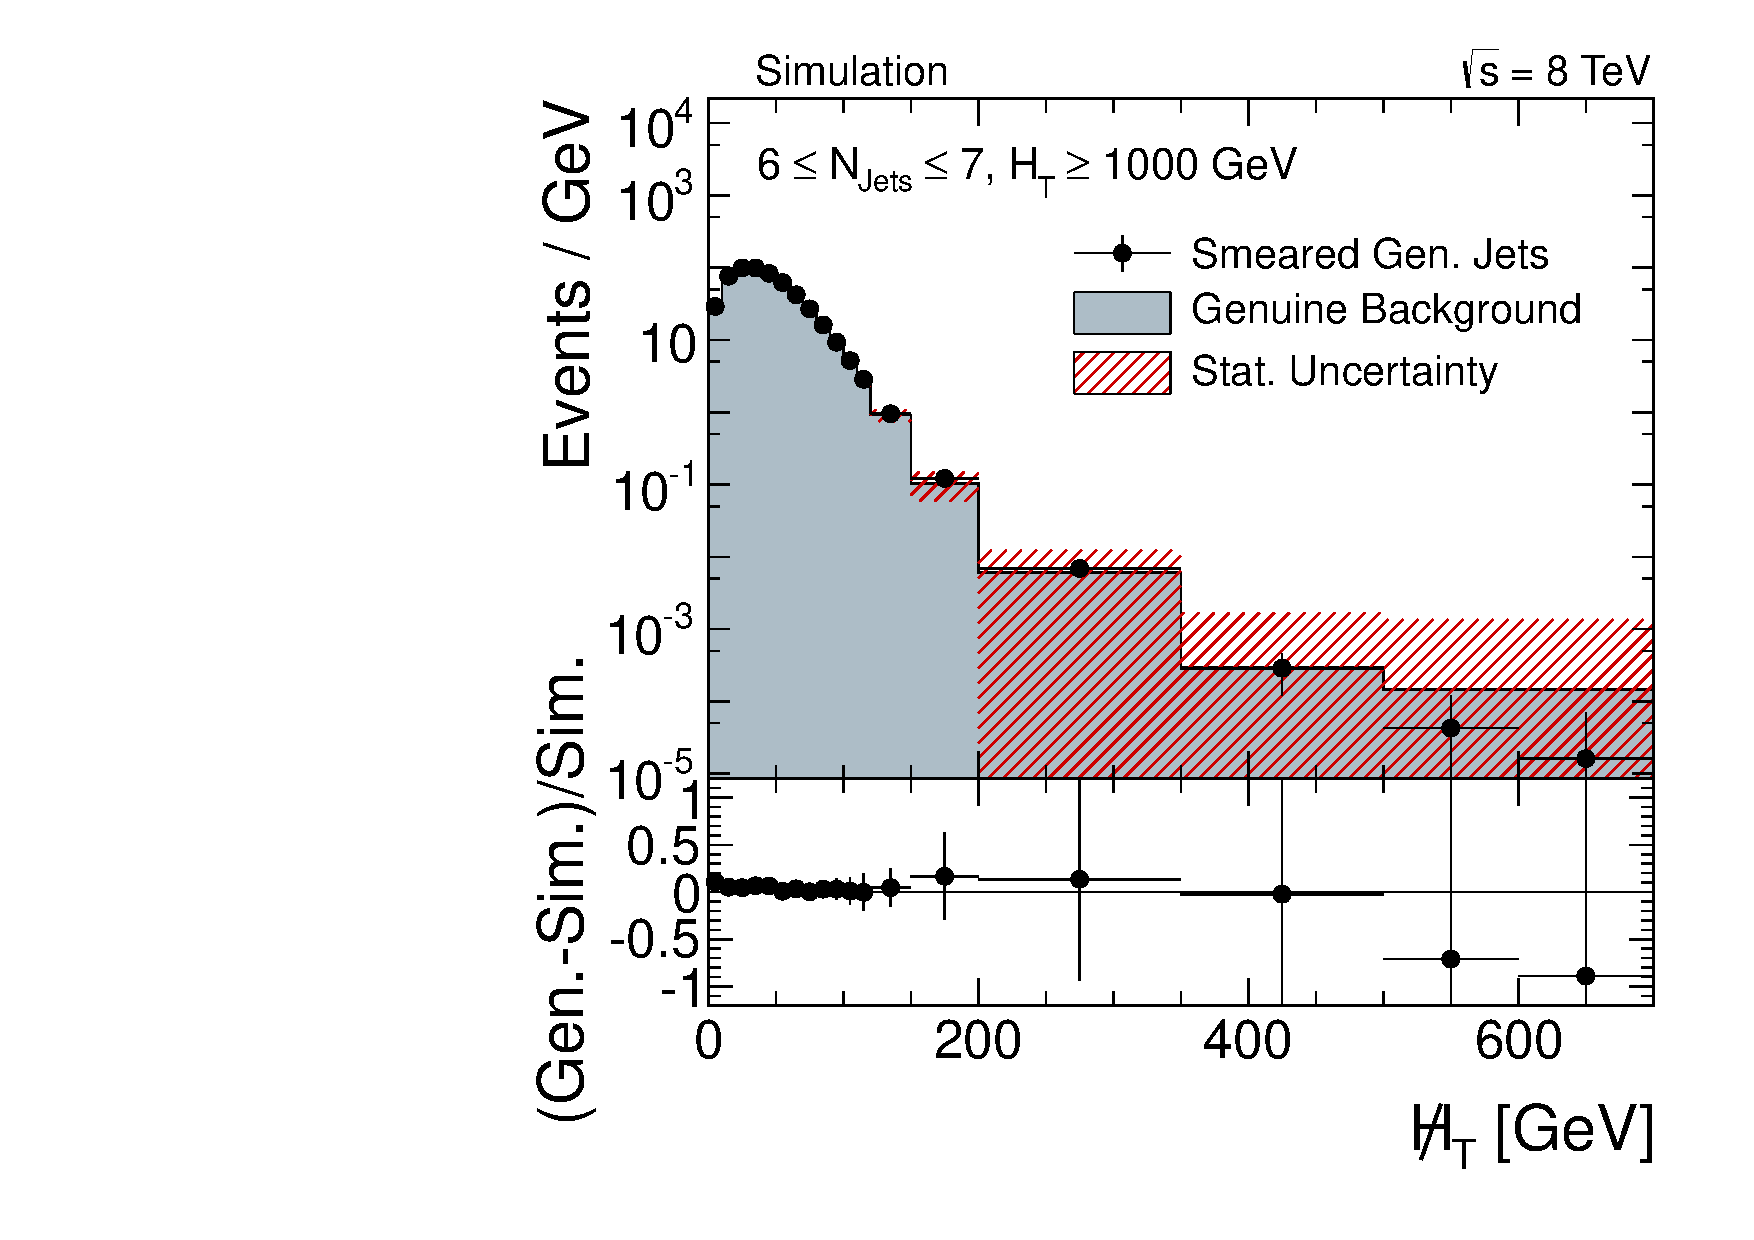
\includegraphics[width=0.49\textwidth]{figures/MHT_JetBin3_HThigh_madgraph_DR53X_chs_withoutPUReweighting_SmearedGenJets_v1.pdf}\\ 
      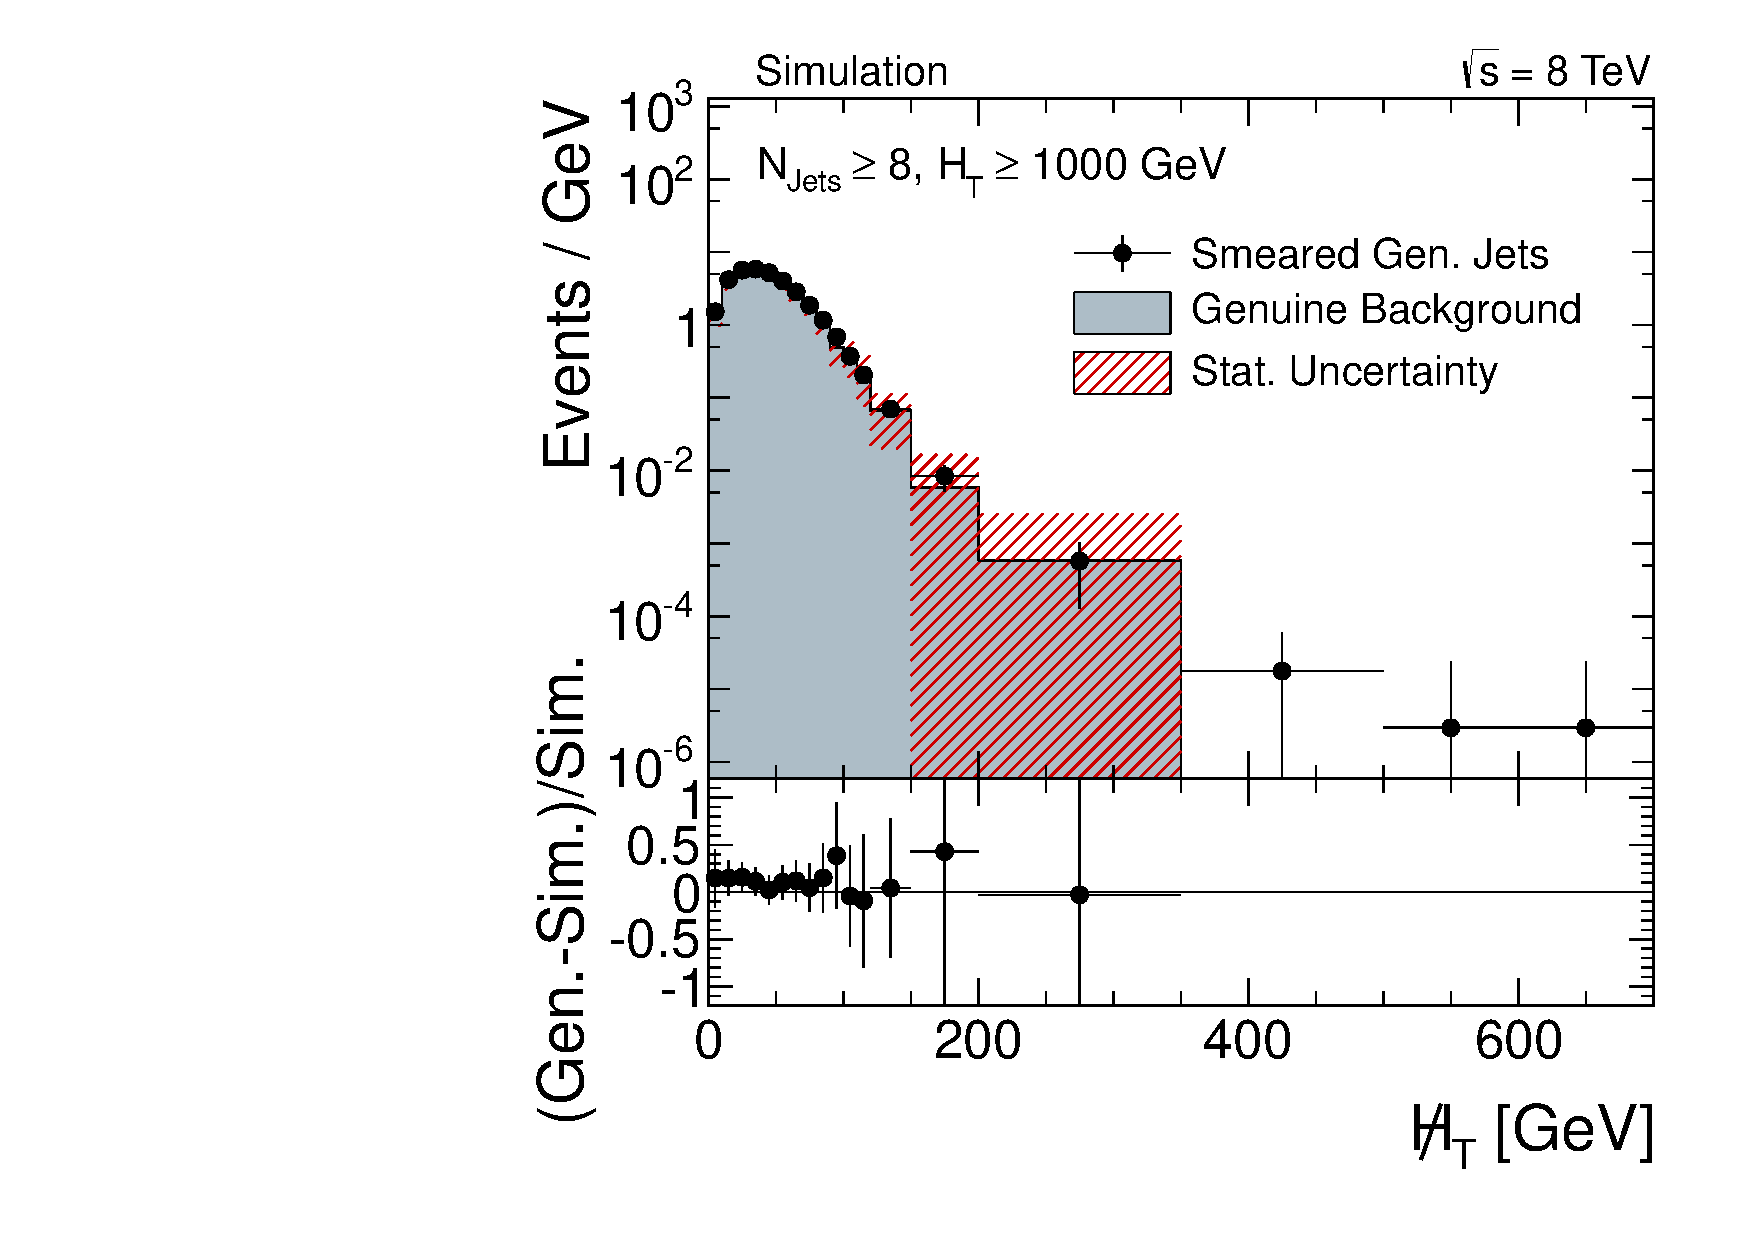
\includegraphics[width=0.49\textwidth]{figures/MHT_JetBin4_HThigh_madgraph_DR53X_chs_withoutPUReweighting_SmearedGenJets_v1.pdf}
    \end{center}
  \end{minipage}
  \caption{Particle-level jets obtained from a QCD multijet sample generated with \madgraph smeared with the truth response templates are compared to the expectation from full simulation. This comparison is shown for search regions with non-negligible QCD multijet background contributions as a function of \MHT defined by $\HT \ge 1000$\gev for $3 \le \NJets \le 5$ (\textit{top left}), $6 \le \NJets \le 7$ (\textit{top right}) and $8 \le \NJets$ (\textit{bottom}) after the application of the minimum $\Delta \phi$ selection.}
  \label{fig:qcd_rs_genjets}
\end{figure}
Overall the distributions derived from the smeared generator jets reproduce nicely the expectation from the simulation. \\
In general, disagreements between predicted and expected quantities in simulated events are in this thesis denoted as \textit{non-closure} of the method and the respective tests of the agreement \textit{closure tests}. Non-closure can occur for instance due to the limited granularity of the response template binning and the averaged flavour composition of the response. In the end, the non-closure of the method is quantified for the whole R+S method including also the rebalancing step (see Sec.~\ref{subsec:RPlusS_app}) and is assigned as systematic uncertainty to the QCD background prediction (see Sec.~\ref{subsec:RA2_syst_unc}). 

%\subsubsection{Feasibility Study of the R+S method}
%\label{subsubsec:qcd_closure_withoutPU}
%\begin{figure}[!t]
%  \centering

%  \begin{minipage}[c]{1.\textwidth}
%    \begin{center}
%      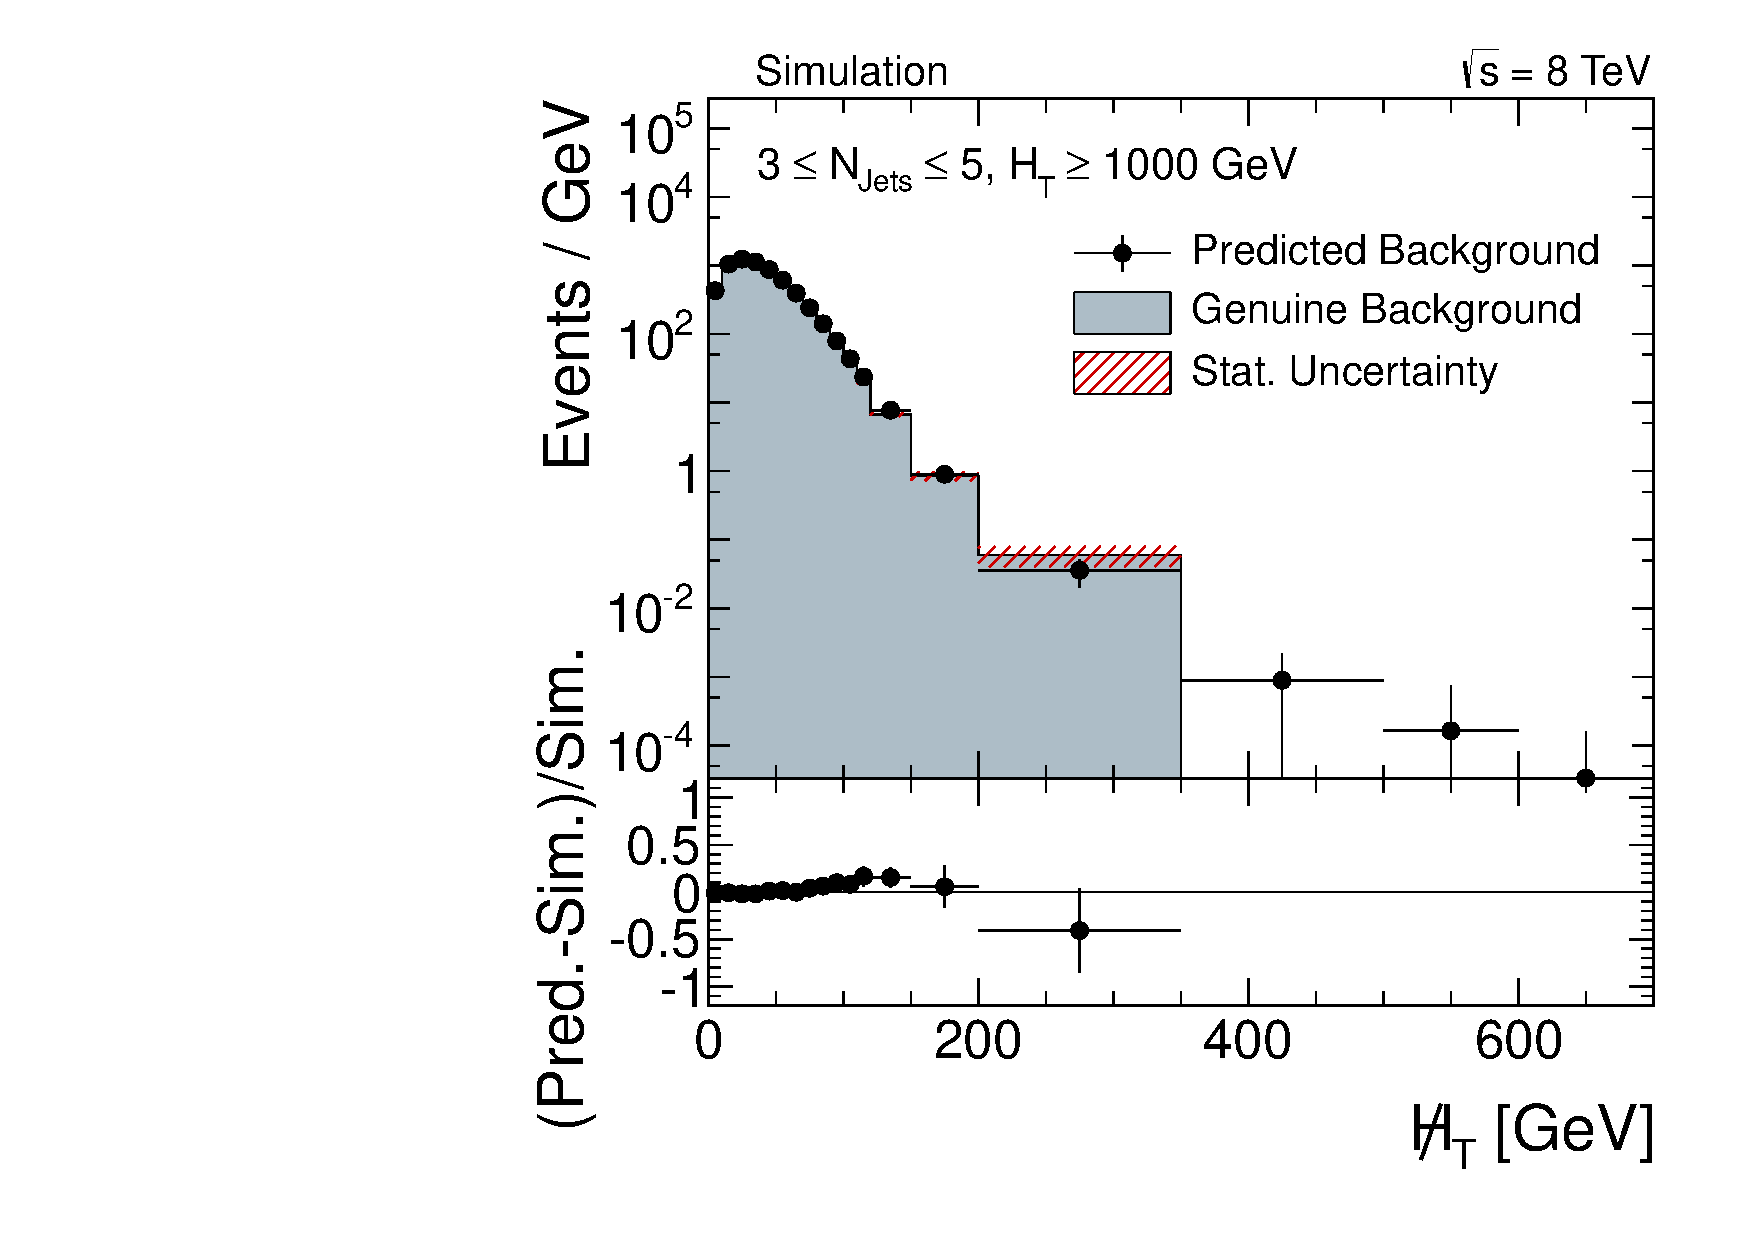
\includegraphics[width=0.49\textwidth]{figures/MHT_JetBin2_HThigh_pythia_chsJets_pt0_NoPU_v1.pdf}% \hspace {1.5 pt} 
%      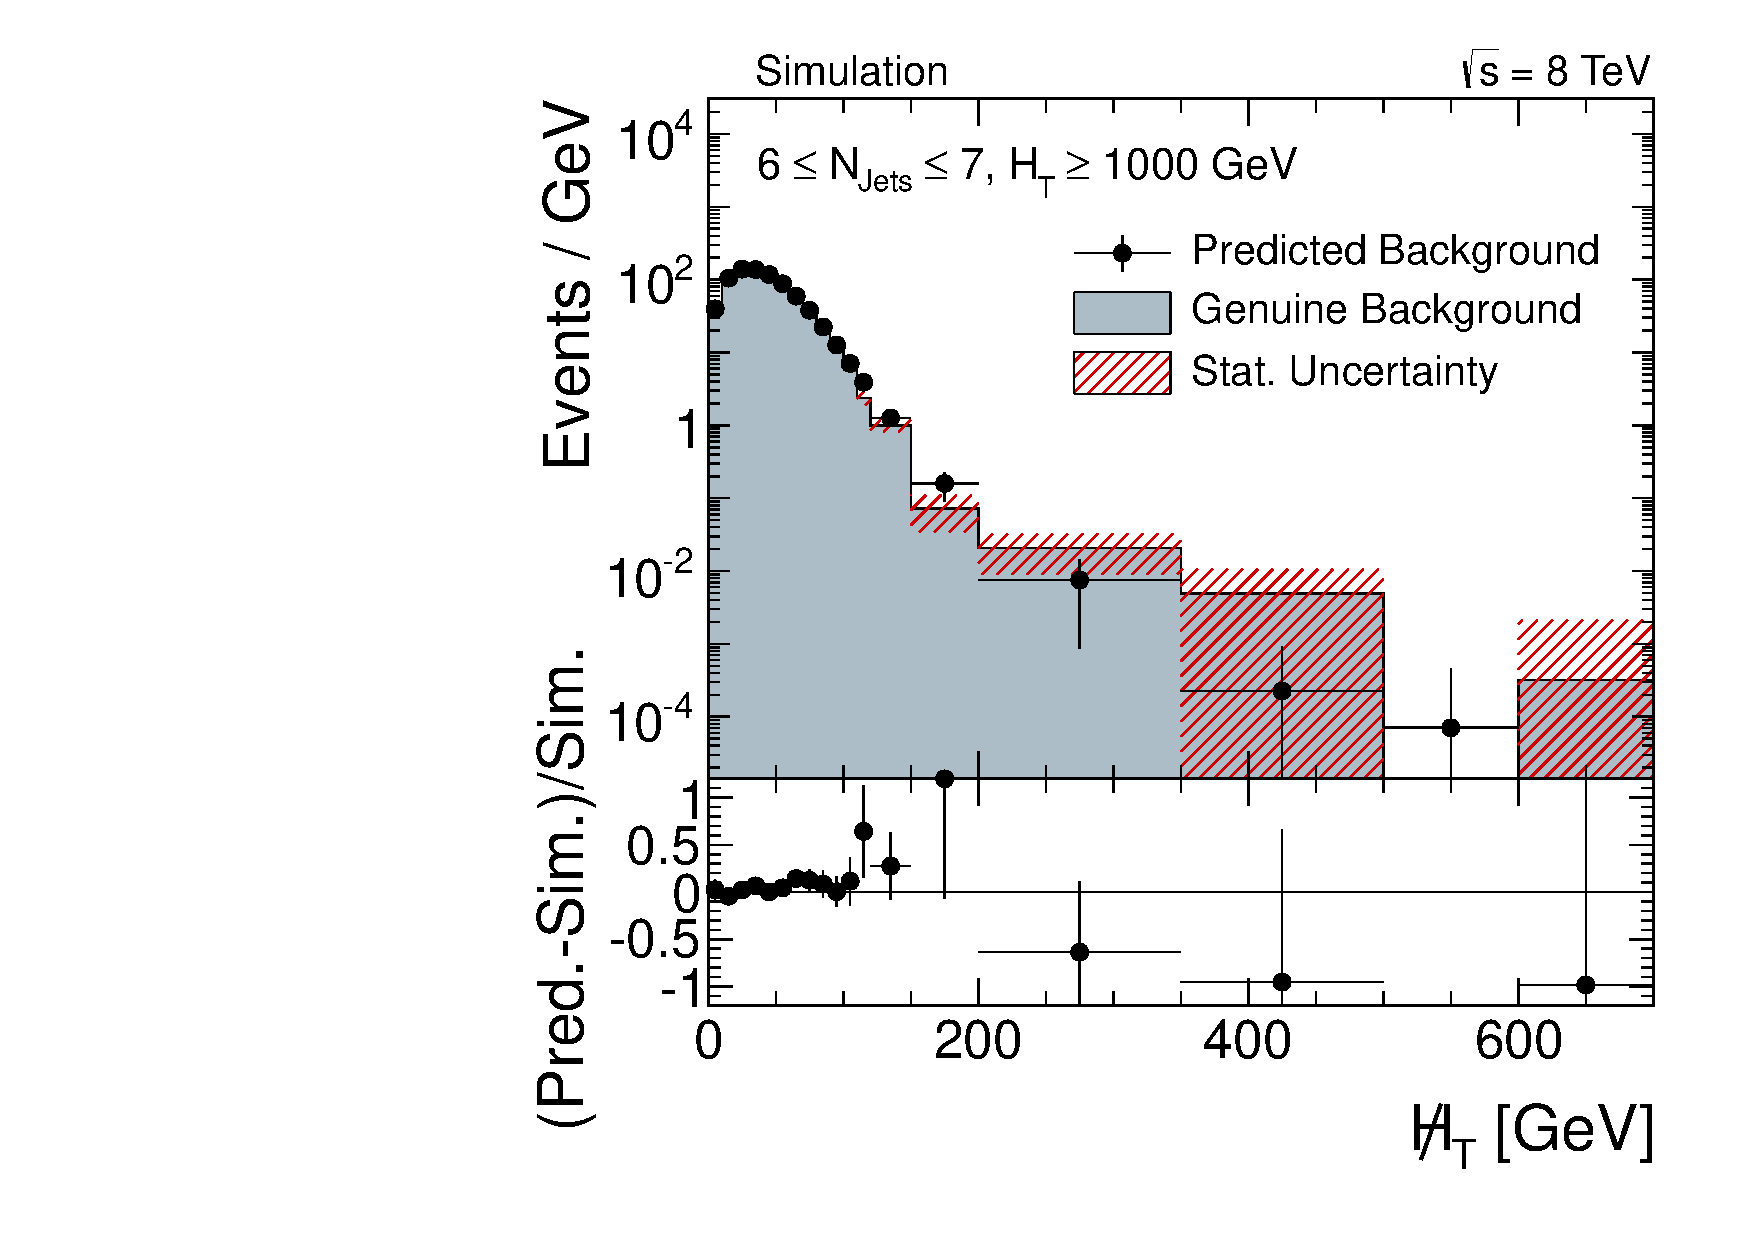
\includegraphics[width=0.49\textwidth]{figures/MHT_JetBin3_HThigh_pythia_chsJets_pt0_NoPU_v1.pdf}\\ 
%      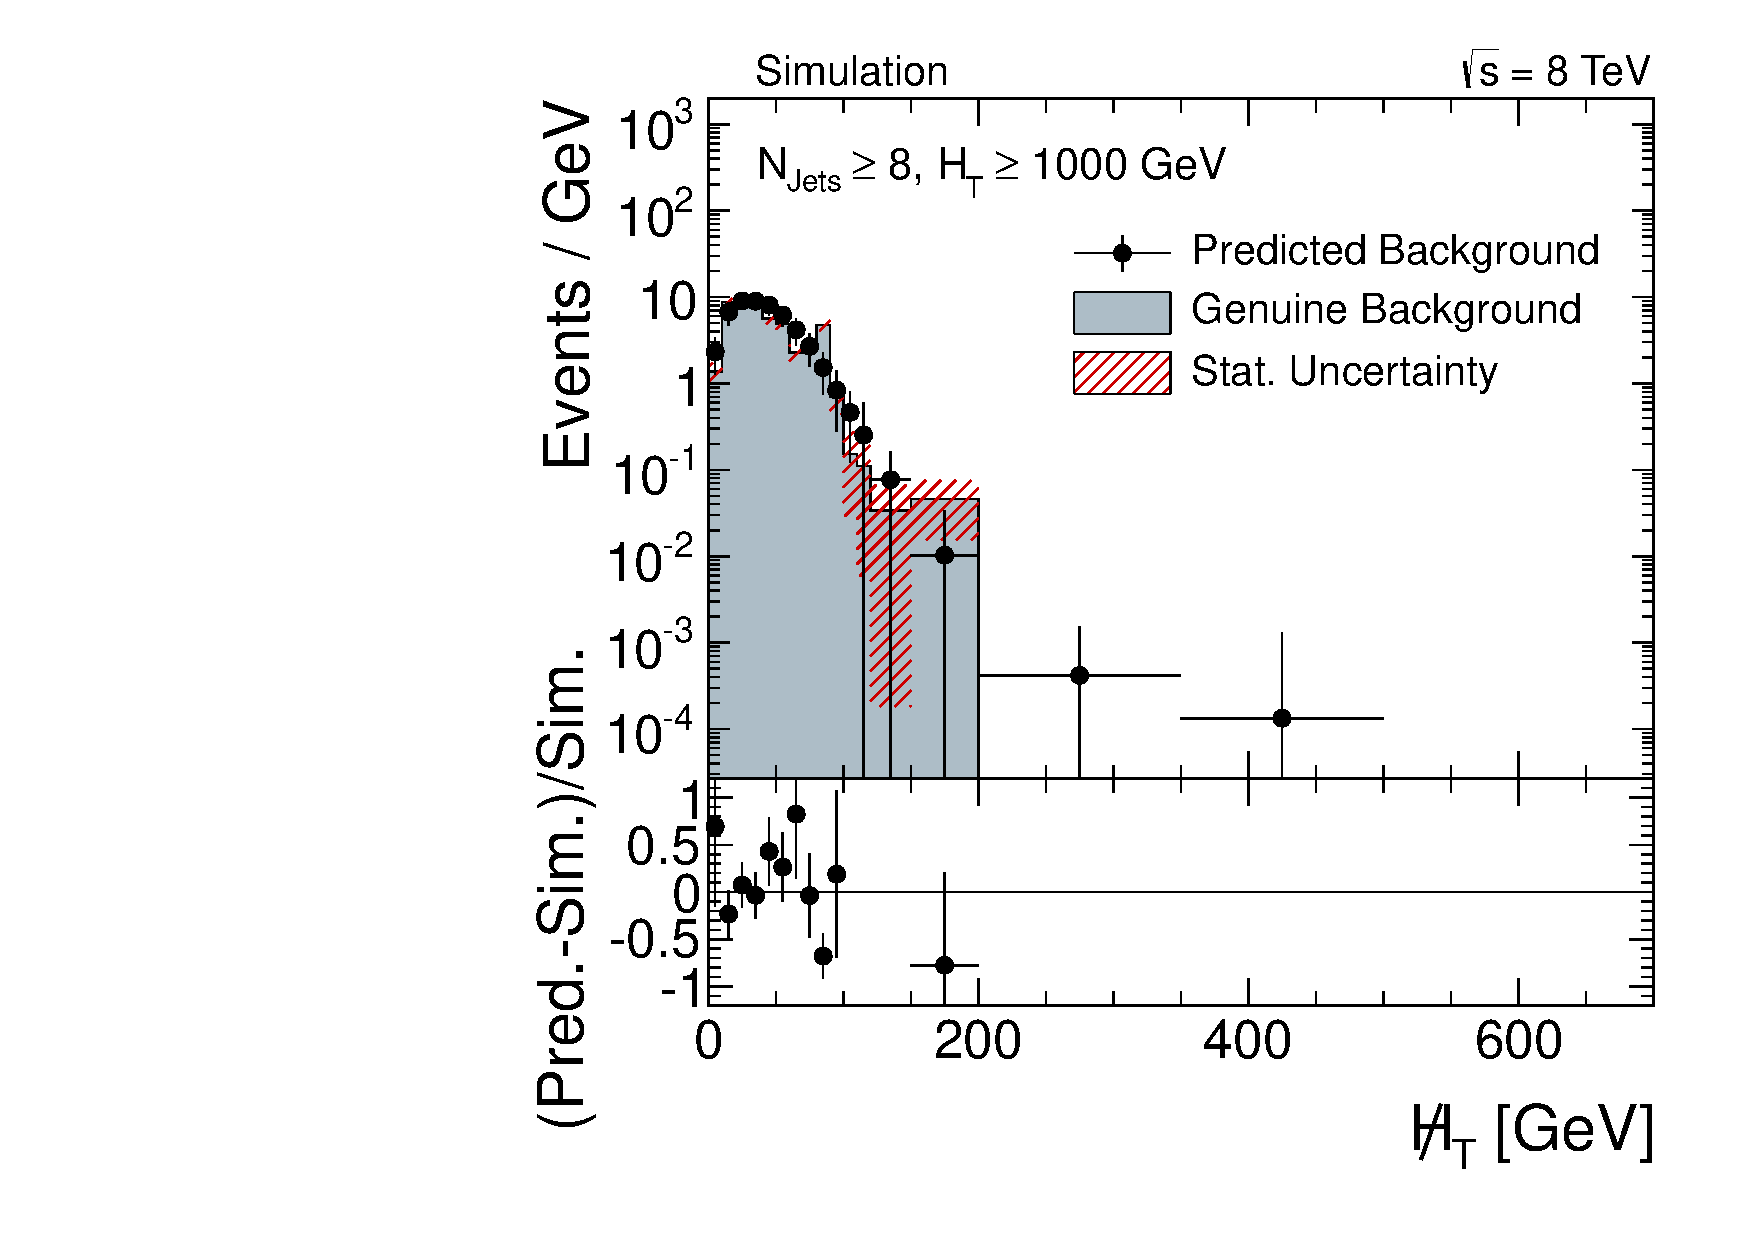
\includegraphics[width=0.49\textwidth]{figures/MHT_JetBin4_HThigh_pythia_chsJets_pt0_NoPU_v1.pdf}
%    \end{center}
%  \end{minipage}
%  \caption{Prediction of QCD background on a QCD multijet sample generated with \pythia \textit{without the simulation of pileup events} compared to the expectation from full simulation. This comparison is shown for search regions with non-negligible QCD multijet background contributions as a function of \MHT defined by $\HT \ge 1000$\gev for $3 \le \NJets \le 5$ (\textit{top left}), $6 \le \NJets \le 7$ (\textit{top right}) and $8 \le \NJets$ (\textit{bottom}) after the application of the minimum $\Delta \phi$ selection.}
%  \label{fig:qcd_rs_closure_nopu}
%\end{figure}
%In order to study the general feasibility of the R+S method to predict background contributions arising from QCD multijet events, the whole procedure is first performed on simulated QCD multijet events \textit{without} simulated pileup events and compared to the expectated event yields. Thus, the events are first reblanced with the kinematic fit adjusting the transverse momenta of all reconstructed jets in the event and then smeared according to the full jet response distribution, as done already for the smearing of generator jets. The resulting QCD background predictions are compared to the expectation in Fig.~\ref{fig:qcd_rs_closure_nopu} for representative search regions with non-negligible QCD background contributions. In general, the disagreement for the actual search regions of $\MHT > 200$\gev is statistically compatible with zero. Thus, the R+S method successfully predicts QCD multijet background in events without additional pileup interactions. The necessary adjustment of the method to realistic collision events is discussed in the next section.

\subsection{Application to Collision Events}
\label{subsec:RPlusS_app} 
The successful performance of the smearing procedure using simulated events, has been shown in the previous section. However, when applying the whole R+S method to collision events including the rebalancing step, further aspects have to be considered. 
\begin{figure}[!t]
  \centering
  \begin{tabular}{cc}
                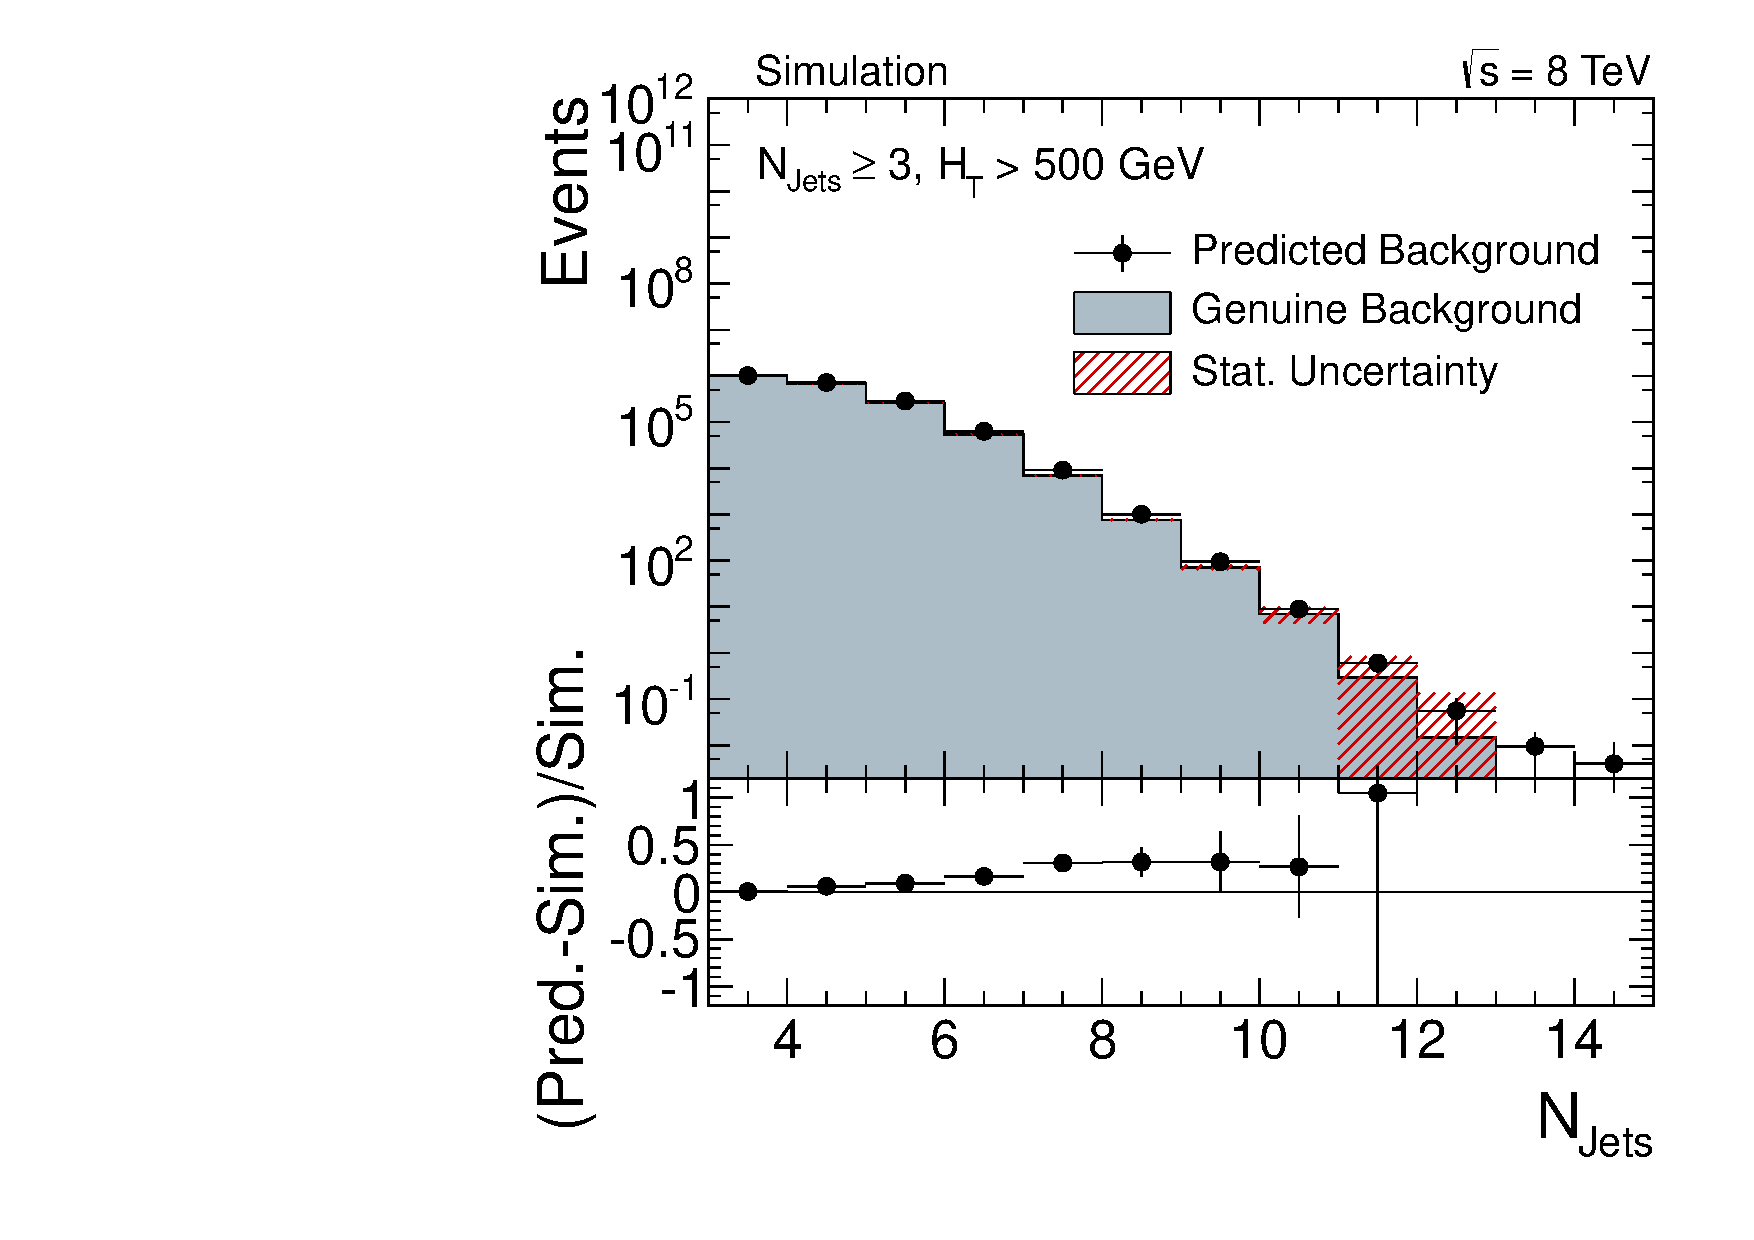
\includegraphics[width=0.49\textwidth]{figures/NJets_baseline_withoutMHT_madgraph_DR53X_chs_TuneZ2star_pt10_withoutPUReweighting_DoNotUseRebCorrection_v1.pdf} &
                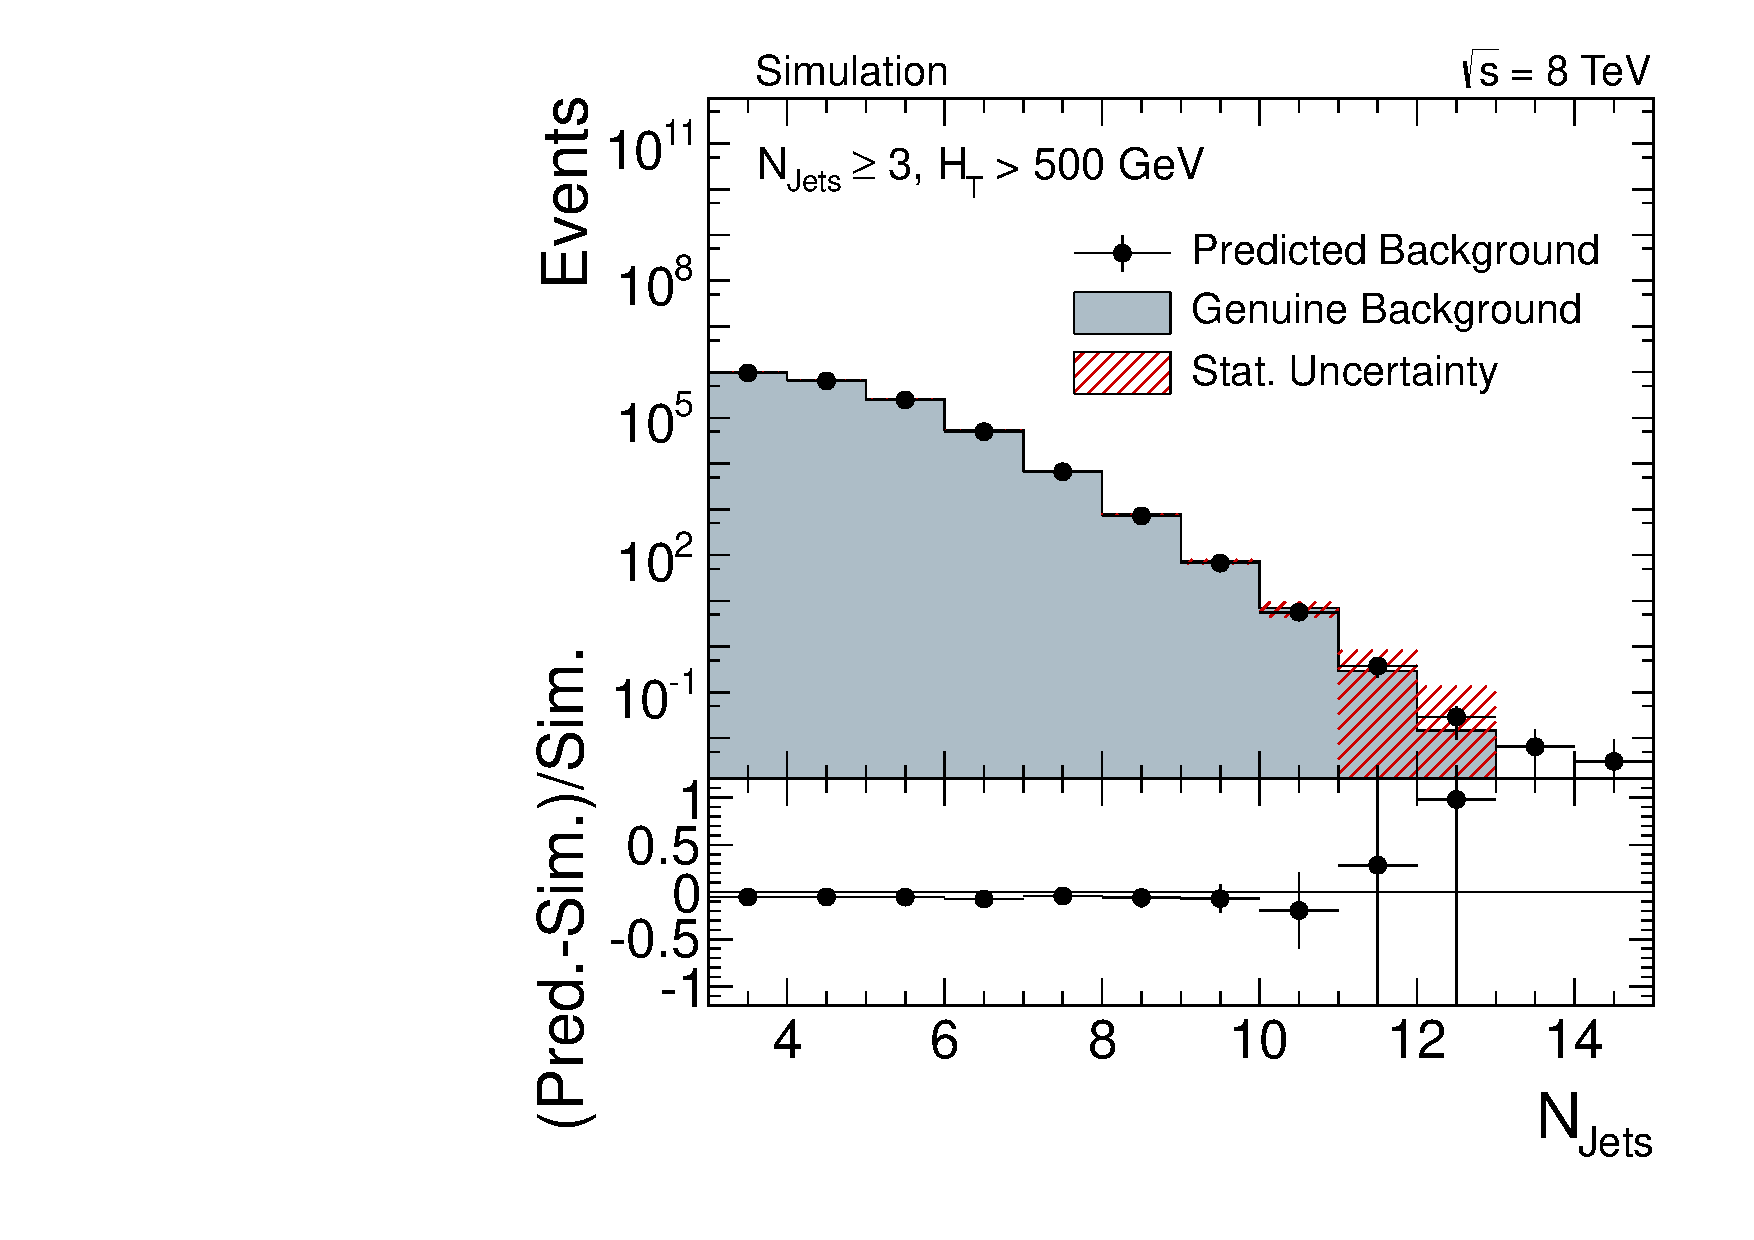
\includegraphics[width=0.49\textwidth]{figures/NJets_baseline_withoutMHT_madgraph_DR53X_chs_TuneZ2star_pt10_withoutPUReweighting_UseRebCorrection_v1.pdf} 

  \end{tabular}
  \caption{Prediction of QCD background on a QCD multijet sample generated with \madgraph compared to the expectation from full simulation with a \pt cut of 10\gev imposed on jets considered in the rebalancing. The predicted $N_{\text{jets}}$ distribution is obtained using the R+S method as in previous versions of the analysis (\textit{left}) and using the R+S method with a correction of the rebalancing step as described in the text (\textit{right}).}
  \label{fig:qcd_rs_rebnjets}
\end{figure}
\\
Jets reconstructed in an event, especially soft jets, do not necessarily originate from the hard interaction, but might arise for instance from pileup or the underlying event. Thus, it is necessary to discard jets below a certain \pt threshold in the rebalancing step in order to not balance them against the hard process. This minimum \pt threshold for jets considered in the rebalancing step can for instance be chosen such that a good inclusive closure of the method in simulated events is observed. Here, only jets with \pt$> 10$\gev are considered for the rebalancing procedure. A similar \pt threshold has also been imposed in earlier versions of the R+S method. There, it has been shown that the R+S method with this configuration provides reliable predictions of \HT and \MHT distributions for an inclusive jet multiplicity selection of $\NJets \ge 3$. Since in the analysis presented in this thesis, the search regions have been extended to several jet multiplicity intervals, it is of particular interest to study, if the R+S method is able to correctly predict the jet multiplicity as well. \\ 
A comparison of the predicted \NJets distribution with the R+S method, using a \pt cut of 10\gev for jets considered in the rebalancing, to the expected genuine background from simulation is shown in Fig.~\ref{fig:qcd_rs_rebnjets} (left) after imposing baseline requirements without the \MHT selection. The distributions exhibit that the R+S method tends to overpredict the expected number of events with increasing jet multiplicities by up to around 40\%. Since the smearing procedure has been shown in Sec.~\ref{subsubsec:qcd_smearing} to provide a reliable performance, this overprediction can be attributed to the rebalancing step. \\
Since the rebalancing step is supposed to provide an estimate of the particle-level jet spectrum, the quality of the rebalancing can be tested by comparing the \pt of the rebalanced jets to the \pt of matched generated jets after performing the rebalancing when excluding jets below 10\gev from the rebalancing procedure. The mean of this ratio, denoted as rebalance factor $\mathrm{f}$, as a function of the momentum of the matched reconstructed jets is shown in Fig.~\ref{fig:qcd_rs_rebfactor}. It is observed that especially jets with small transverse momentum (\pt $\leq$ 100 GeV) are, on average, rebalanced to too high momenta. The observed too high momenta of rebalanced jets, thus result in more jets passing the \NJets threshold of 50\gev than expected. As a consequence, the number of predicted QCD events in the higher jet multiplicity bins is too large. 
\begin{figure}[!t]
  \centering
  \begin{tabular}{c}
                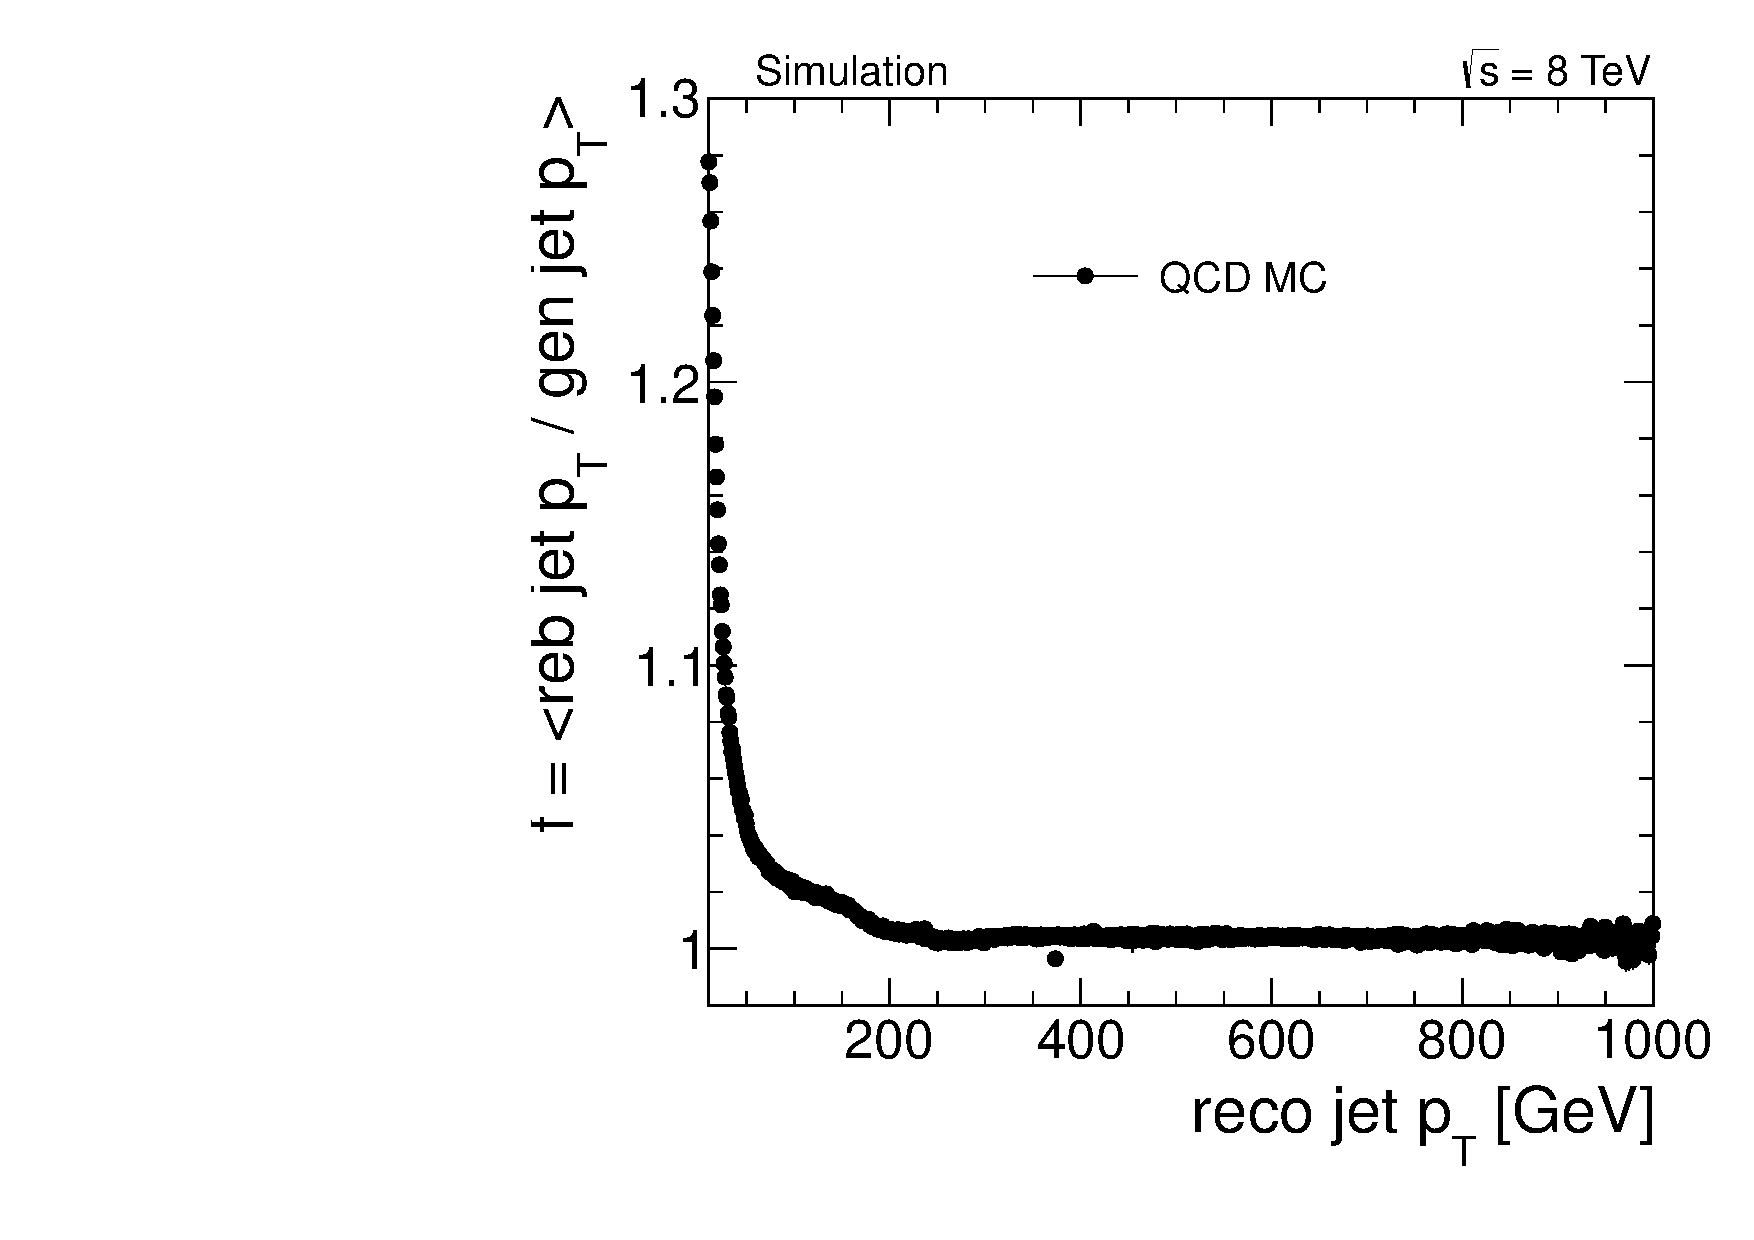
\includegraphics[width=0.49\textwidth]{figures/RebalanceCorrectionFactors_DR53X_chsJets_TuneZ2star_withoutPUReweighting_pt10_vsRecoMadgraph.pdf} 
  \end{tabular}
  \caption{Mean of transverse momenta of rebalanced jets divided by transverse momenta of matched generated jets as a function of transverse momentum of matched reonstructed jets obtained from simulated events generated with \madgraph.}
  \label{fig:qcd_rs_rebfactor}
\end{figure}
\\
This effect can be explained by the necessity to discard soft jets in the rebalancing procedure. By not taking into account all jets in the rebalancing, also soft jets that do belong to the actual hard interaction are not considered. This introduces an artifical additional imbalance in the event which has to be compensated for in the kinematic fit. In order to further study this threshold effect, a closure test is performed on a simulated QCD sample which is generated without pileup. This offers the possibility to drop the requirement of $\pt > 10$\gev for jets considered in the rebalancing and is obtained from the \textsc{Pythia6}~\cite{Sjostrand:2006za} event generator with tune Z2*~\cite{Chatrchyan:2013gfi}. For consistency, also the response templates are in this closure test taken from the same QCD sample. The results of this test are shown in Fig.~\ref{fig:qcd_rs_closure_nopu}. In general, the disagreement for the shown regions is statistically compatible with zero. Especially the higher jet multiplicities are in this case predicted correctly by the R+S method, when there is no necessity to impose the minimum \pt threshold in the rebalancing. 
 \begin{figure}[!t]
  \centering

  \begin{minipage}[c]{1.\textwidth}
    \begin{center}
      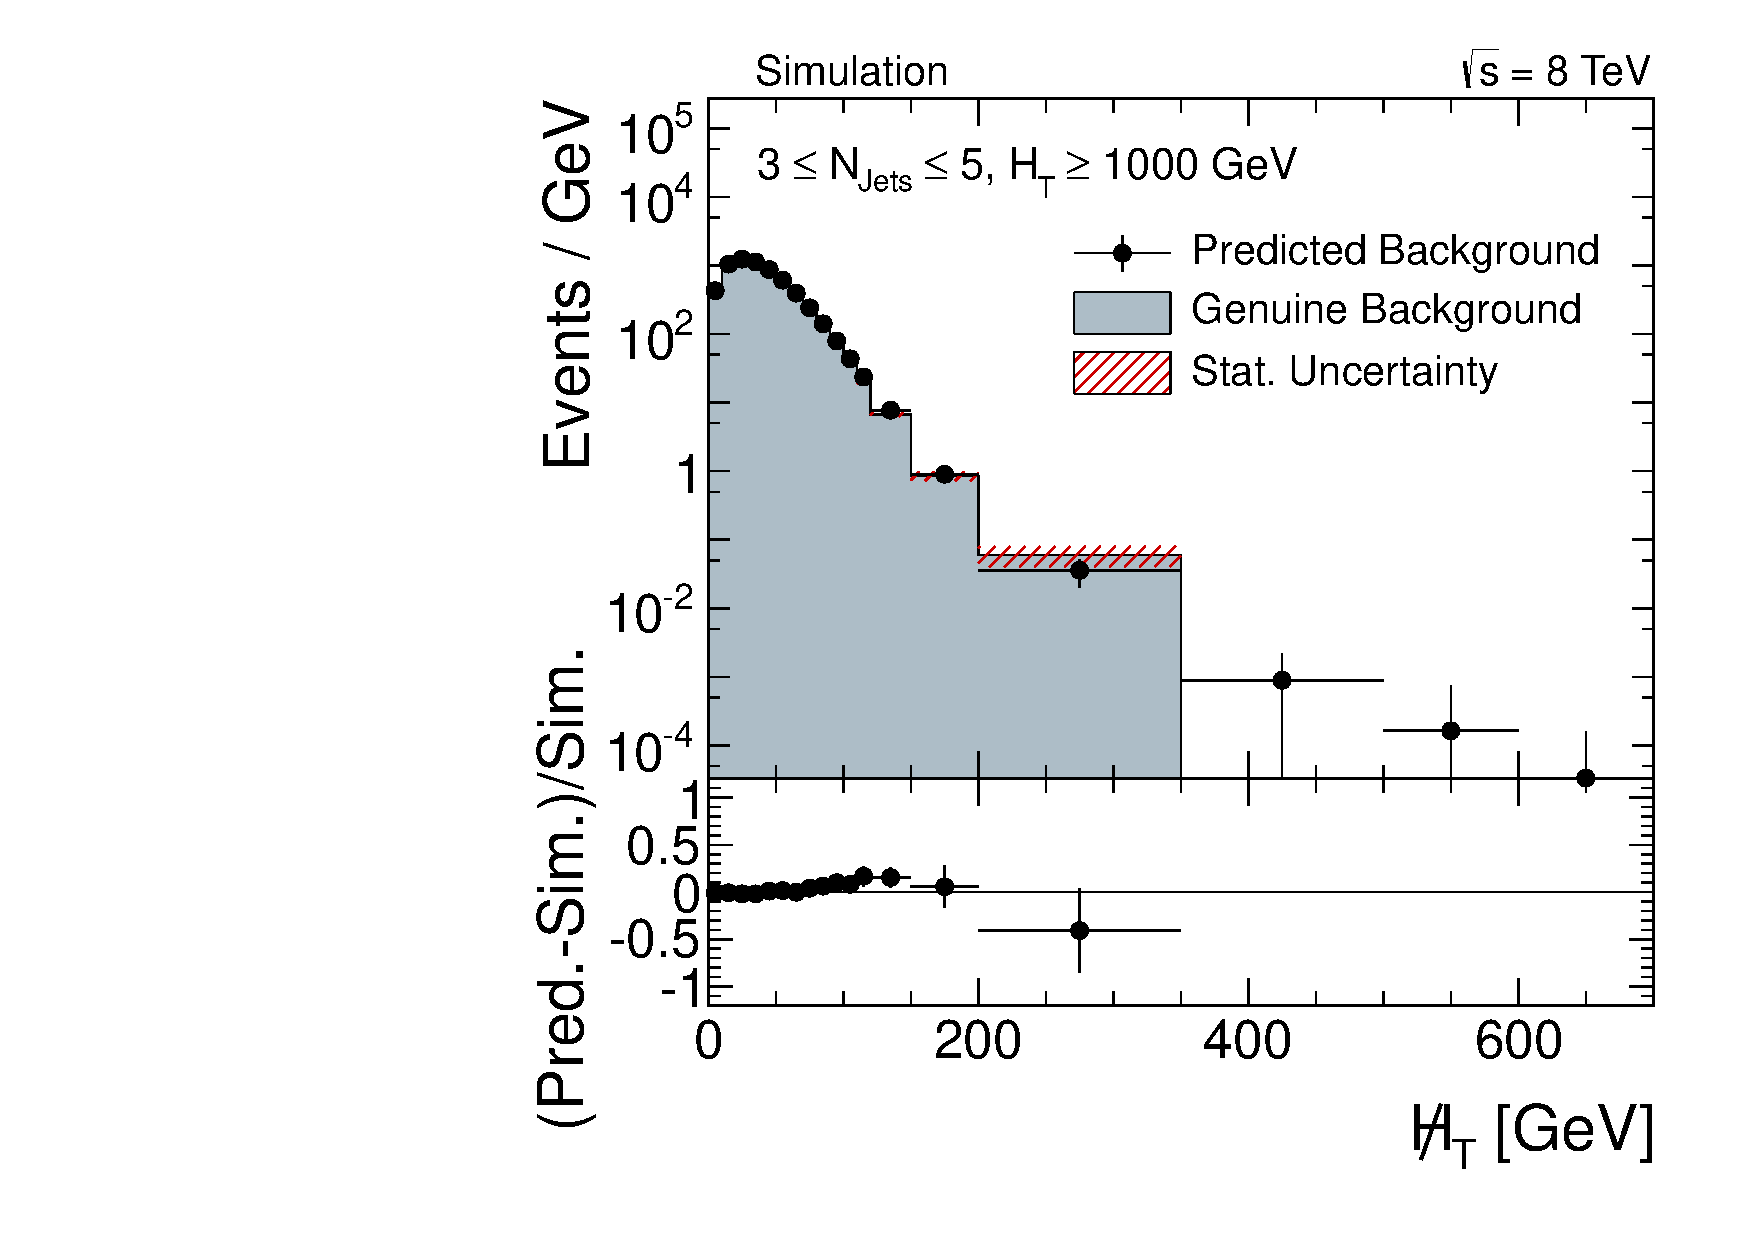
\includegraphics[width=0.49\textwidth]{figures/MHT_JetBin2_HThigh_pythia_chsJets_pt0_NoPU_v1.pdf}% \hspace {1.5 pt} 
      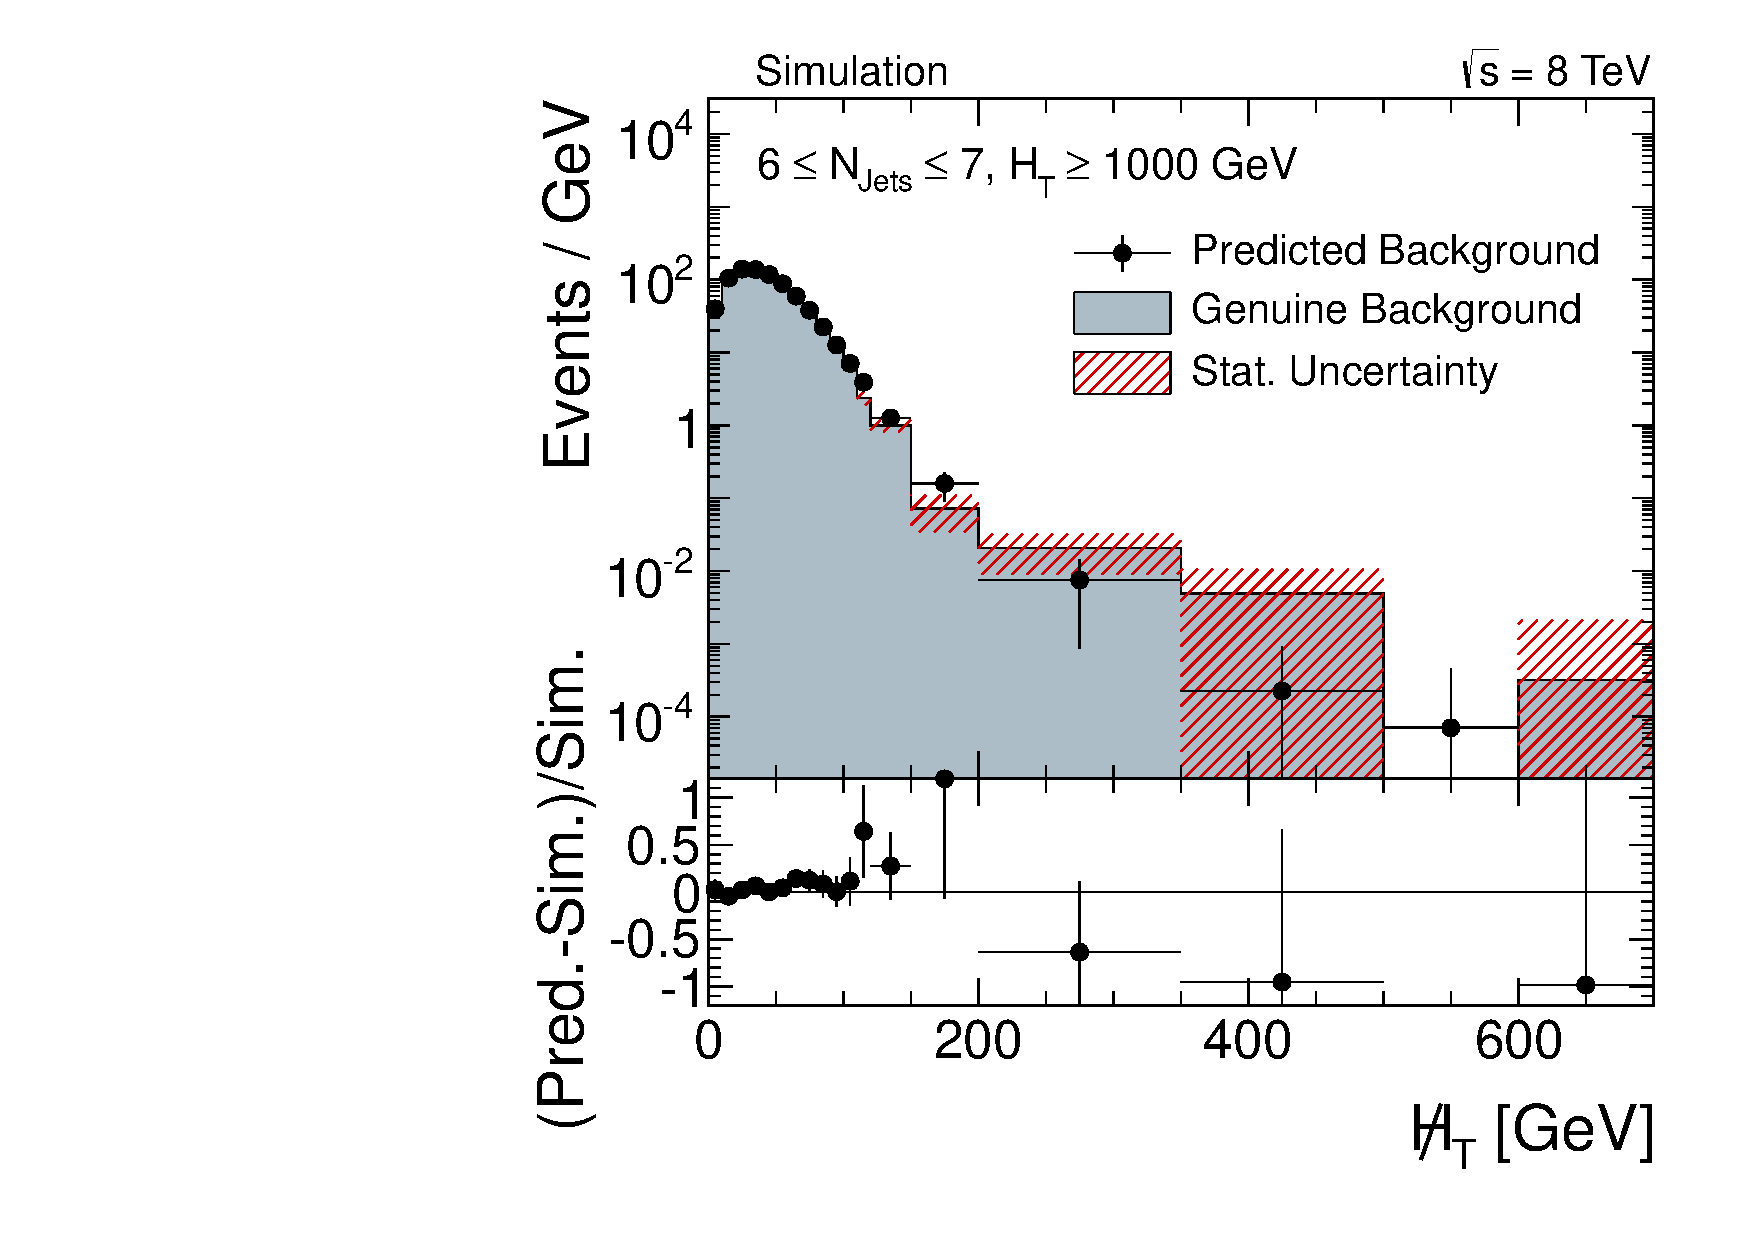
\includegraphics[width=0.49\textwidth]{figures/MHT_JetBin3_HThigh_pythia_chsJets_pt0_NoPU_v1.pdf}\\ 
      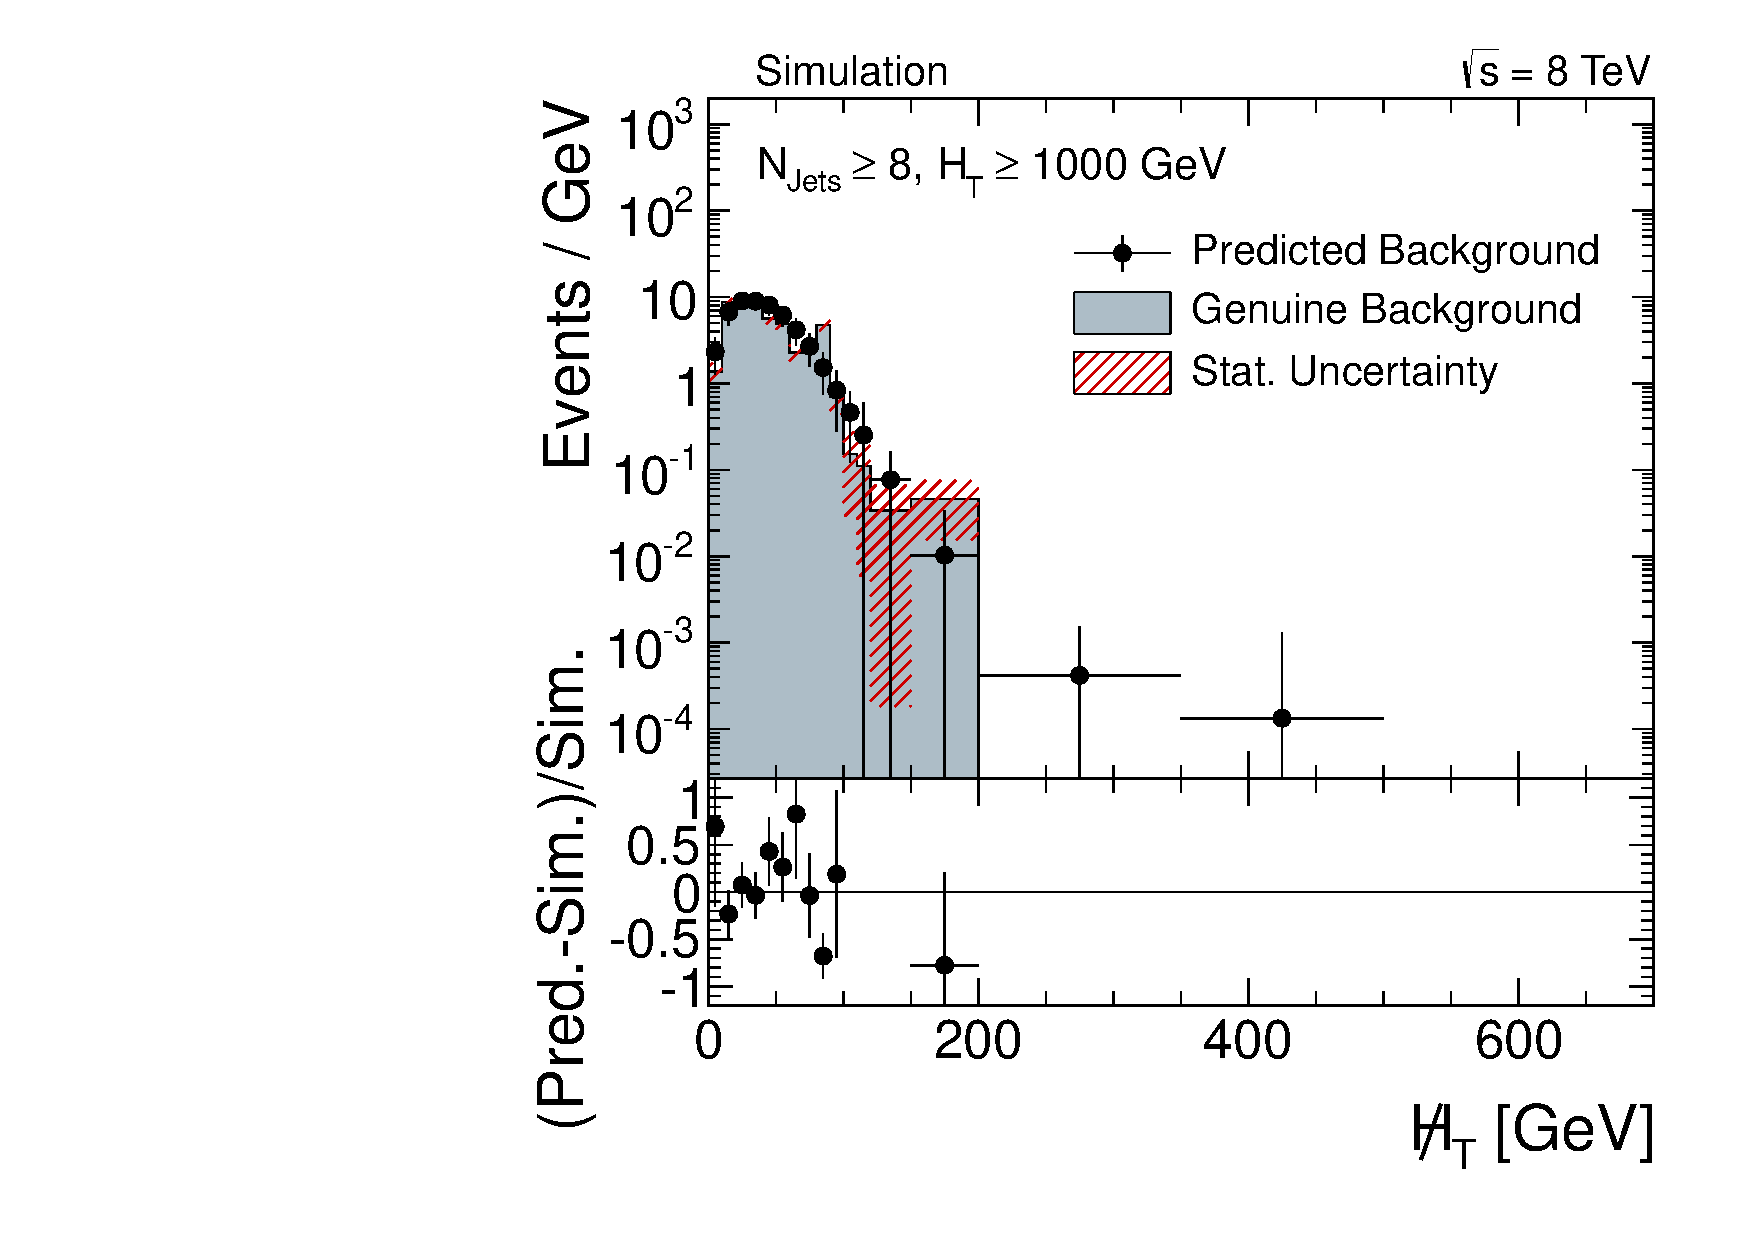
\includegraphics[width=0.49\textwidth]{figures/MHT_JetBin4_HThigh_pythia_chsJets_pt0_NoPU_v1.pdf}
    \end{center}
  \end{minipage}
  \caption{Prediction of QCD background on a QCD multijet sample generated with \pythia without the simulation of pileup compared to the expectation from full simulation. This comparison is shown as a function of \MHT for regions defined by $\HT \ge 1000$\gev and $3 \le \NJets \le 5$ (\textit{top left}), $6 \le \NJets \le 7$ (\textit{top right}) or $8 \le \NJets$ (\textit{bottom}) after applying the minimum $\Delta \phi$ selection.}
  \label{fig:qcd_rs_closure_nopu}
\end{figure}
\\
In order to account for the observed threshold effect in events in which the minimum \pt selection in the rebalancing actually is needed, an empirical correction factor is introduced. The correction factor is employed such that in the rebalancing procedure each jet momentum is scaled by $1/\mathrm{f}$ before the kinematic fit is performed. Thus, the effect of overpredicting the jet momenta of jets with small transverse momenta is taken care of by downscaling the jet momenta before the kinematic fit by a factor representing the average overprediction. The prediction of the \NJets distribution with the adjusted R+S method compared to the expected background is shown in Fig.~\ref{fig:qcd_rs_rebnjets} (right) and illustrates that the regulated method leads to correct predictions of the QCD event yields also in the high jet multiplicity regions. The correction factor derived from simulation is later also applied to the rebalancing of data events, since in data the same minimum jet-\pt threshold of 10\gev is chosen.% \\
%The correction factor is derived by using generator-truth information and hence can only be determined on simulated event samples. However, this can be done for different samples to study, if the correction is somewhat generator dependent. The rebalance correction factor is thus derived for the QCD multijet samples obtained from \pythia and \madgraph. The difference of the correction factors derived from these two samples is found to be of the order of $1-2\%$ cf. Fig.~\ref{fig:qcd_rs_rebfactor} (left). In addition, the correction factor was also determined for different bins of primary vertices and thus for different pile-up conditions. It is observed that the functional form of the correction factor is independent of the pile-up conditions cf. Fig.~\ref{fig:qcd_rs_rebfactor} (right). This justifies the assumption that the observed harder jet \pt-spectrum after the rebalancing step without the application of correction factor is due to the acceptance of the jet \pt cut on the jets considered for the rebalancing. 

\subsection{Validation in Simulated Events}
\label{subsec:validation_mc}
The quality of the R+S method to predict background contributions from QCD multijet events is tested on simulated samples by several closure tests in different kinematic regions. In these tests, the data-based prediction is applied to simulated events and compared to the results from full simulation, as explained in Sec.~\ref{subsec:RPlusS_app}. The different closure tests as a function of \MHT for various jet multiplicity bins for a low \HT $= [500, 1000]$\gev and a high \HT $\ge 1000$\gev selection are shown in Fig.~\ref{fig:qcd_rs_closure} for simulated events obtained from \madgraph. In general, the prediction shows a good agreement with the expected QCD background contributions. Nonetheless, deviations between prediction and expectation occur. These are considered as remaining bias of the R+S method and treated as systematic uncertainty. Due to the limited statistics of the simulated sample, the bias uncertainty is not evaluated for each search region individually, but for the different jet multiplicity intervals and a low and a high \HT selection, corresponding to the kinematic regions defined in Fig.~\ref{fig:qcd_rs_closure}.
\begin{figure}[!hp]
  \centering
  \begin{tabular}{cc}
                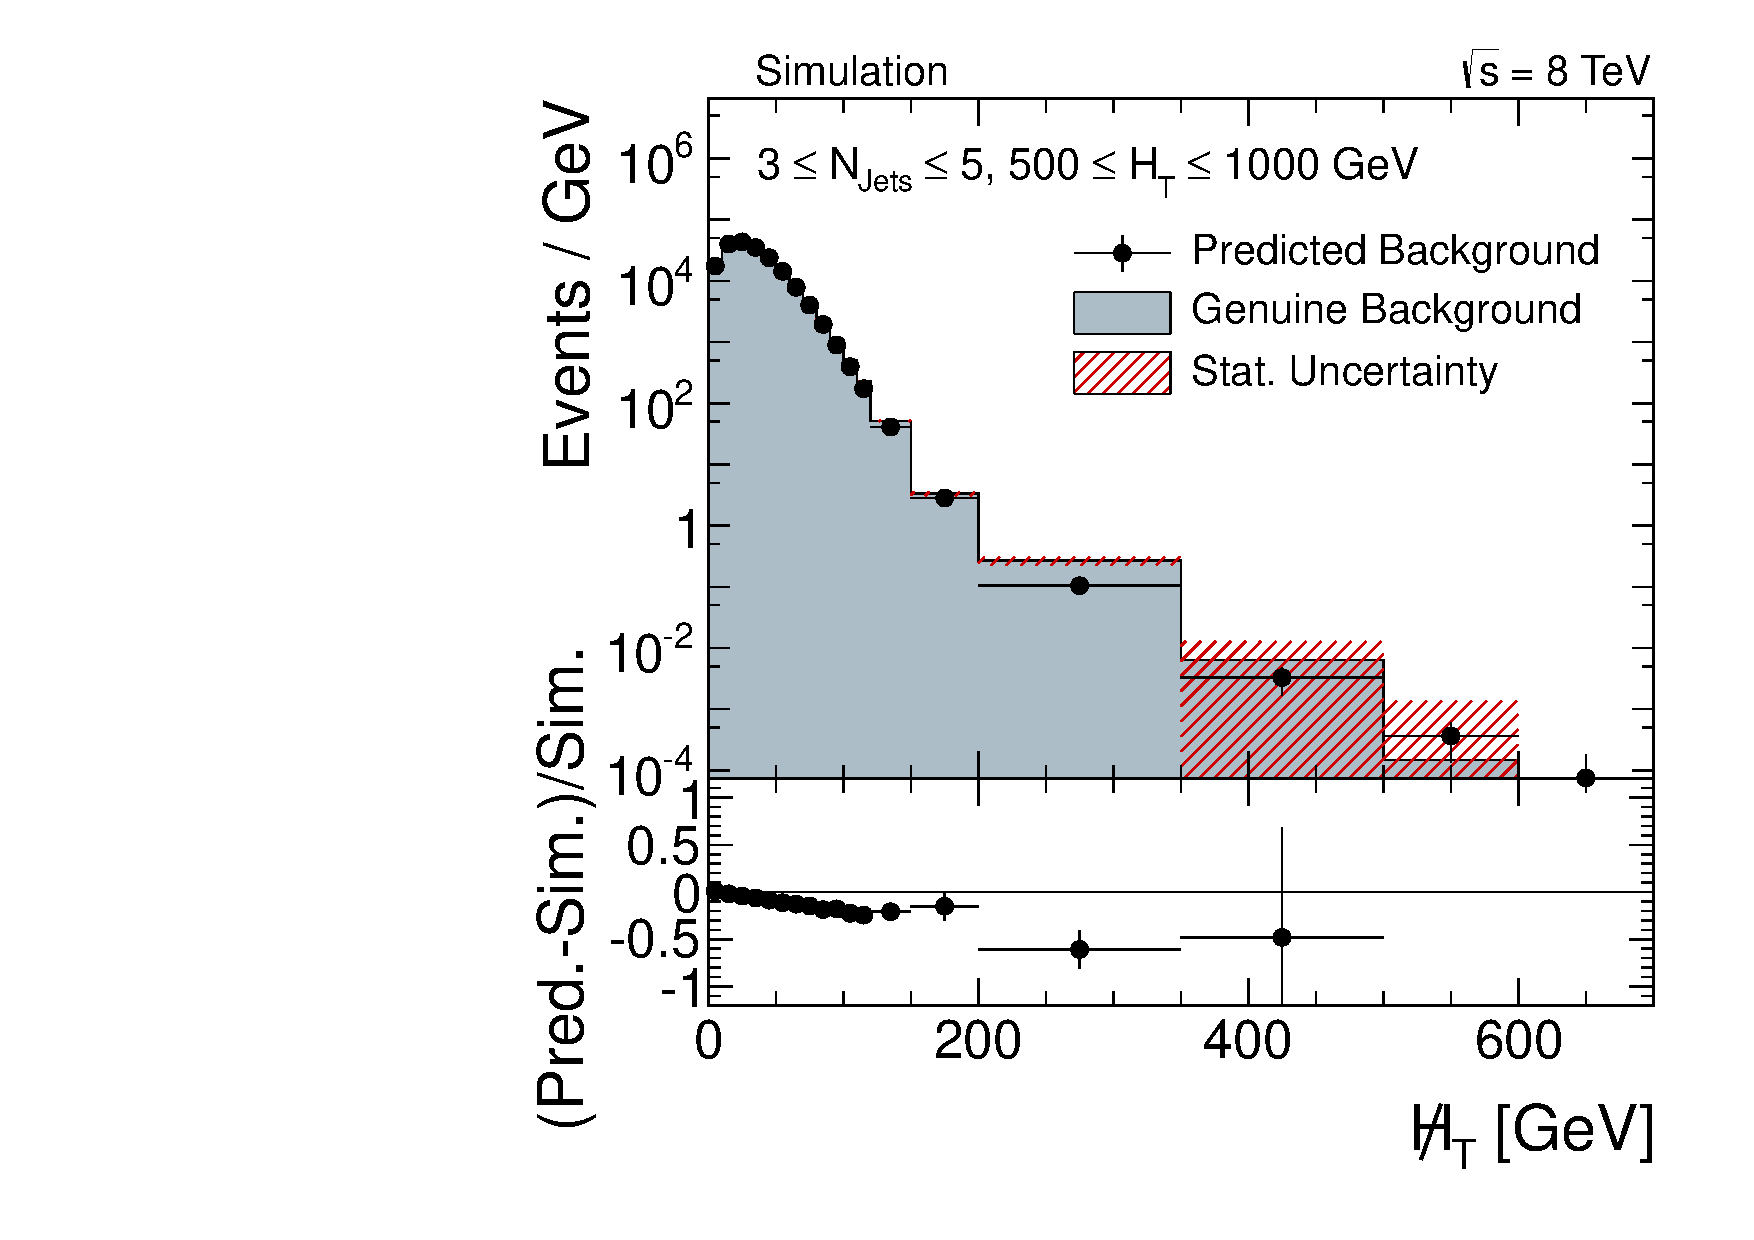
\includegraphics[width=0.49\textwidth]{figures/MHT_JetBin2_HTlow_madgraph_DR53X_chs_TuneZ2star_pt10_withoutPUReweighting_UseRebCorrection_v1.pdf} &
                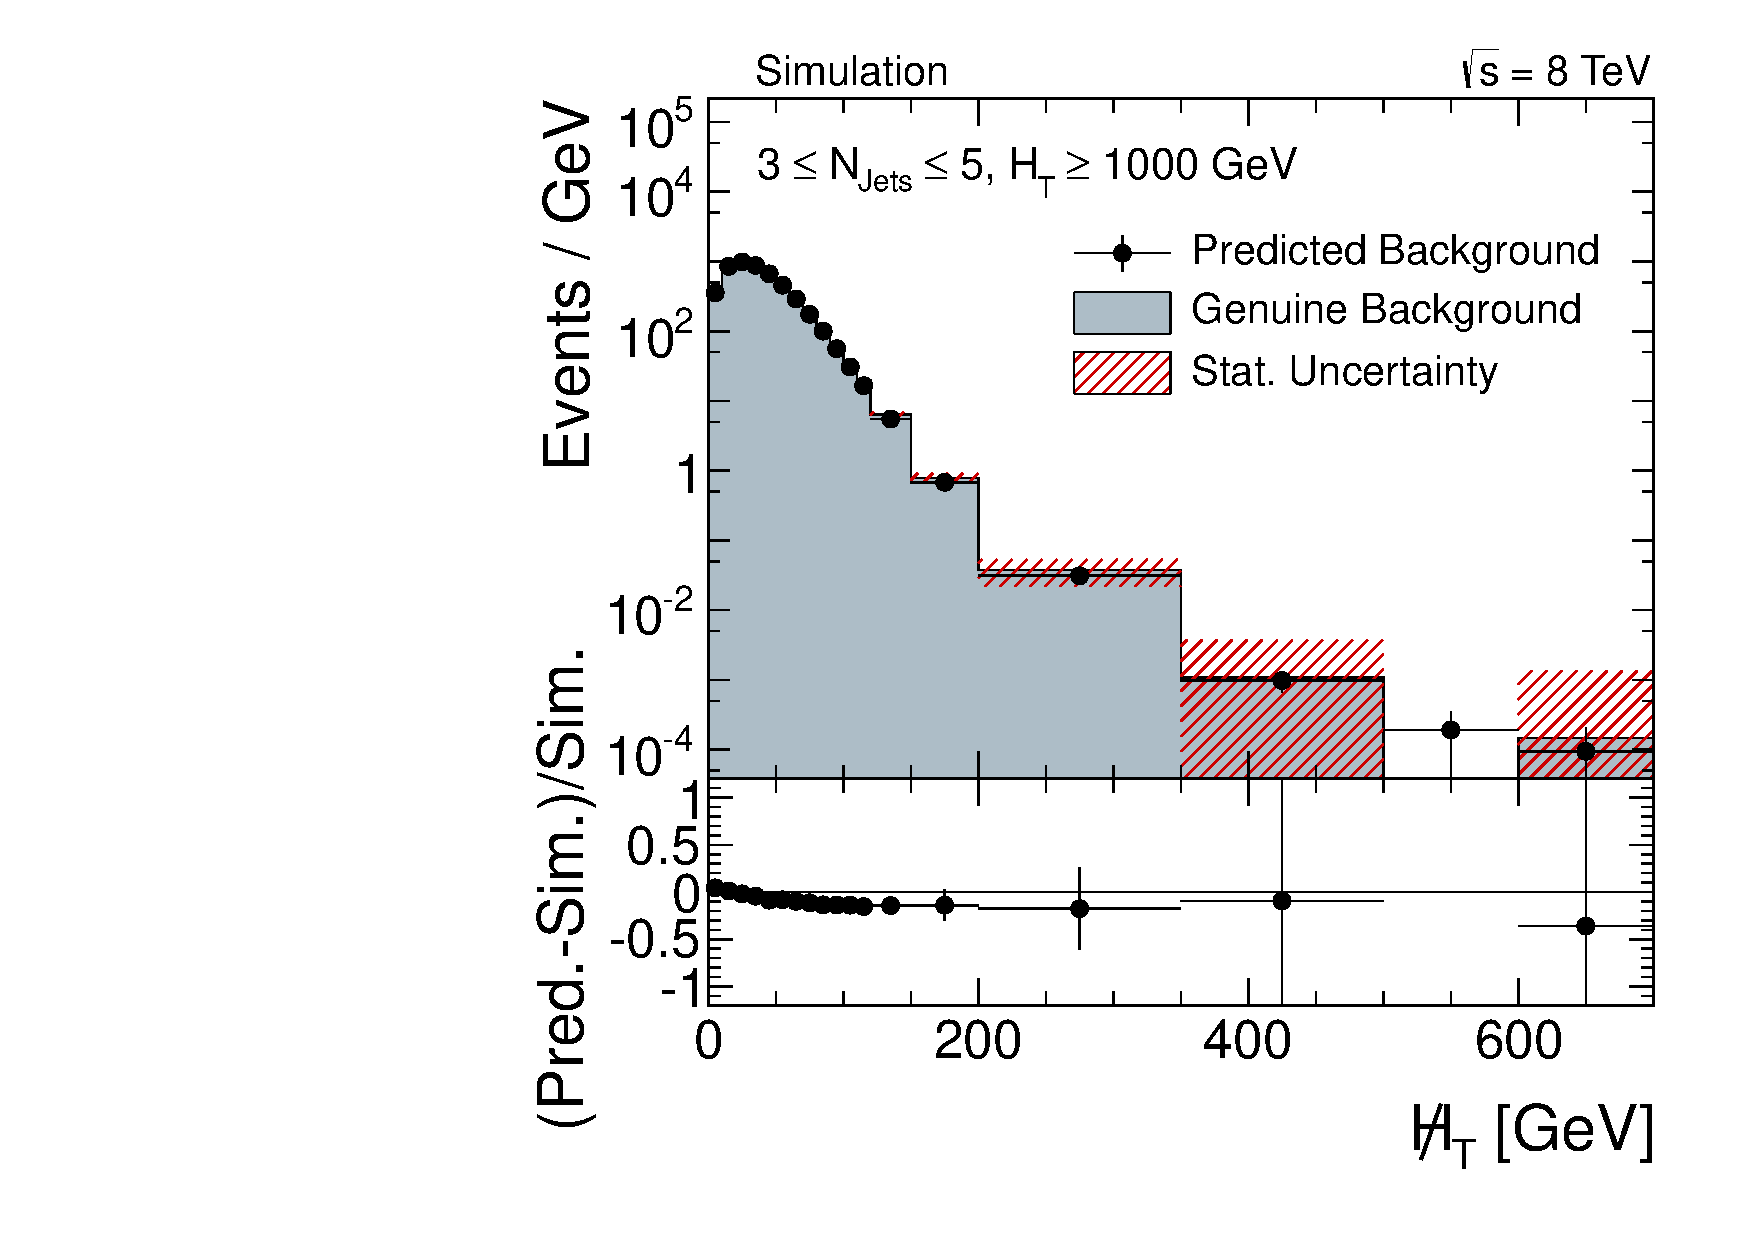
\includegraphics[width=0.49\textwidth]{figures/MHT_JetBin2_HThigh_madgraph_DR53X_chs_TuneZ2star_pt10_withoutPUReweighting_UseRebCorrection_v1.pdf}\\
                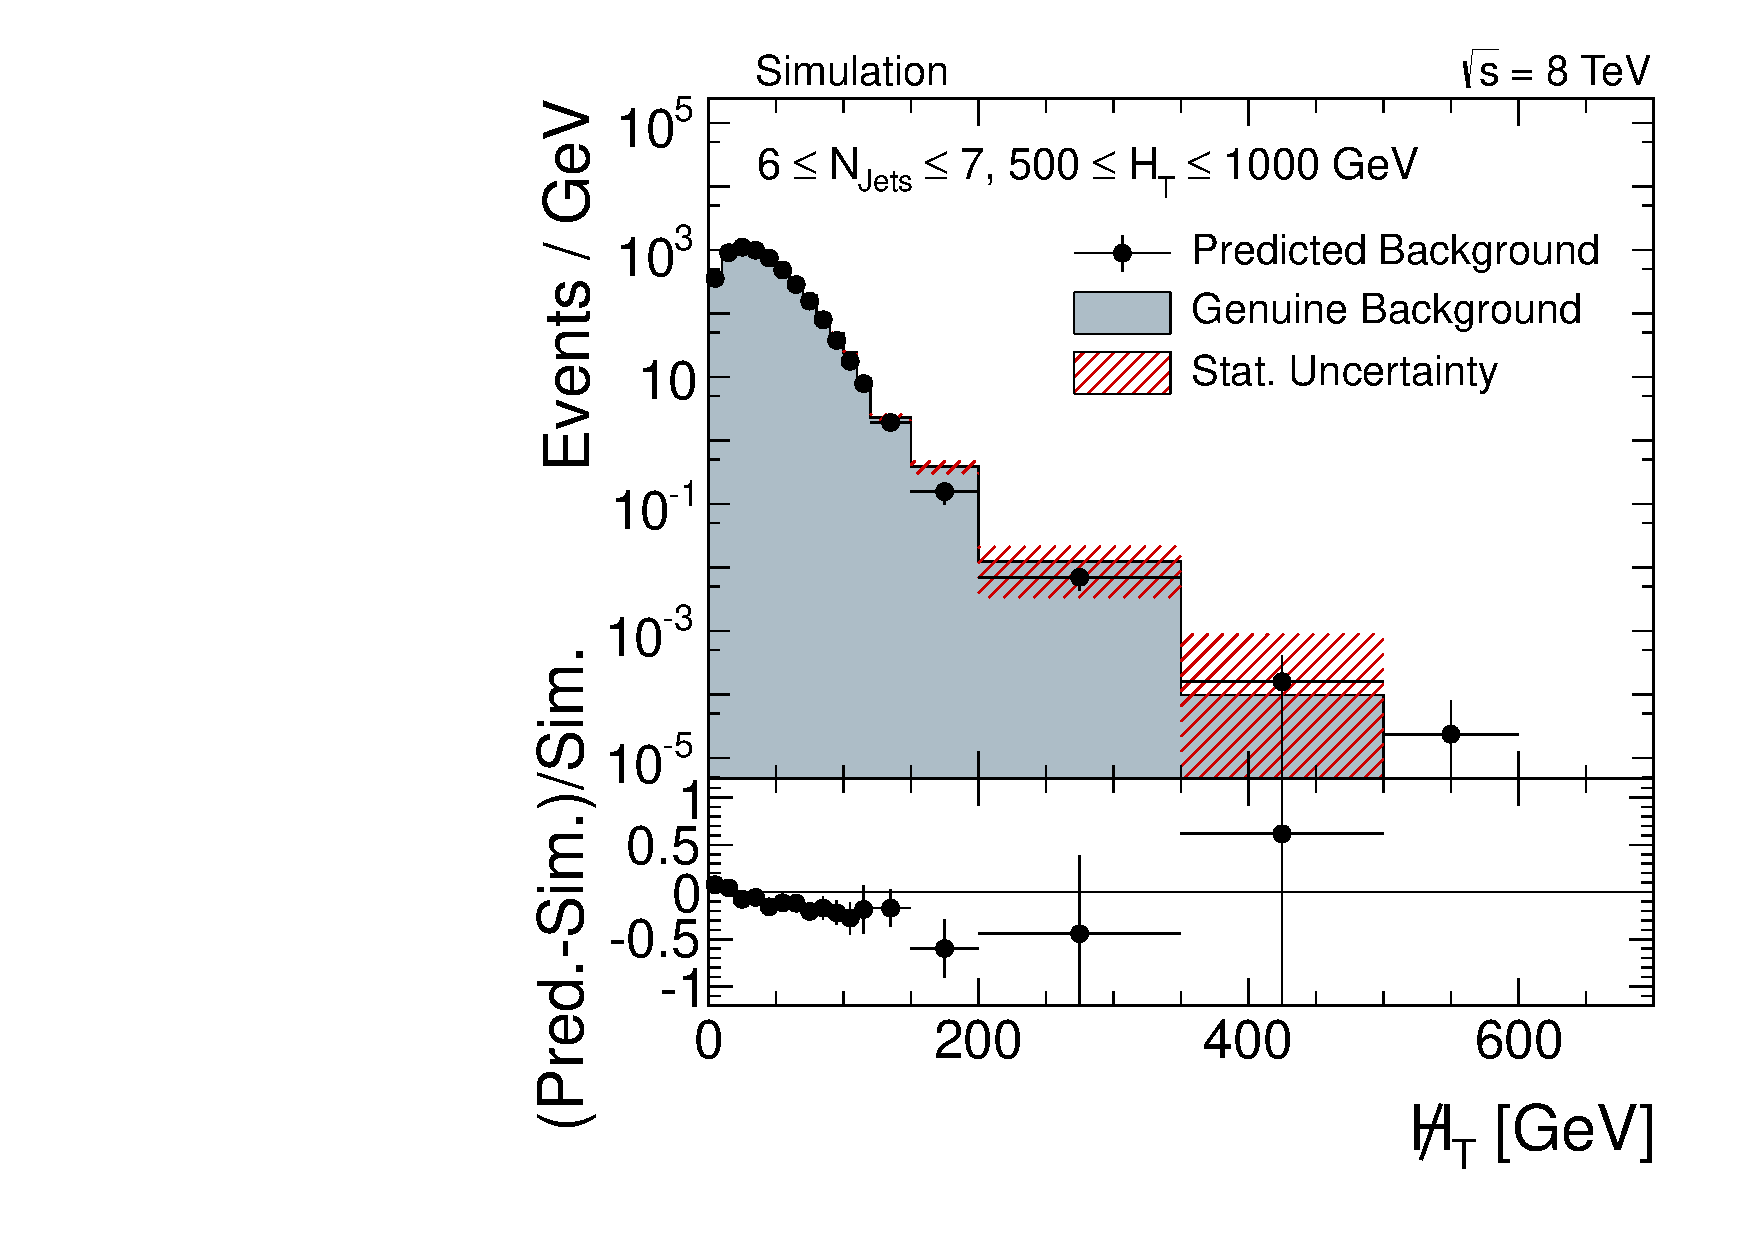
\includegraphics[width=0.49\textwidth]{figures/MHT_JetBin3_HTlow_madgraph_DR53X_chs_TuneZ2star_pt10_withoutPUReweighting_UseRebCorrection_v1.pdf} &
                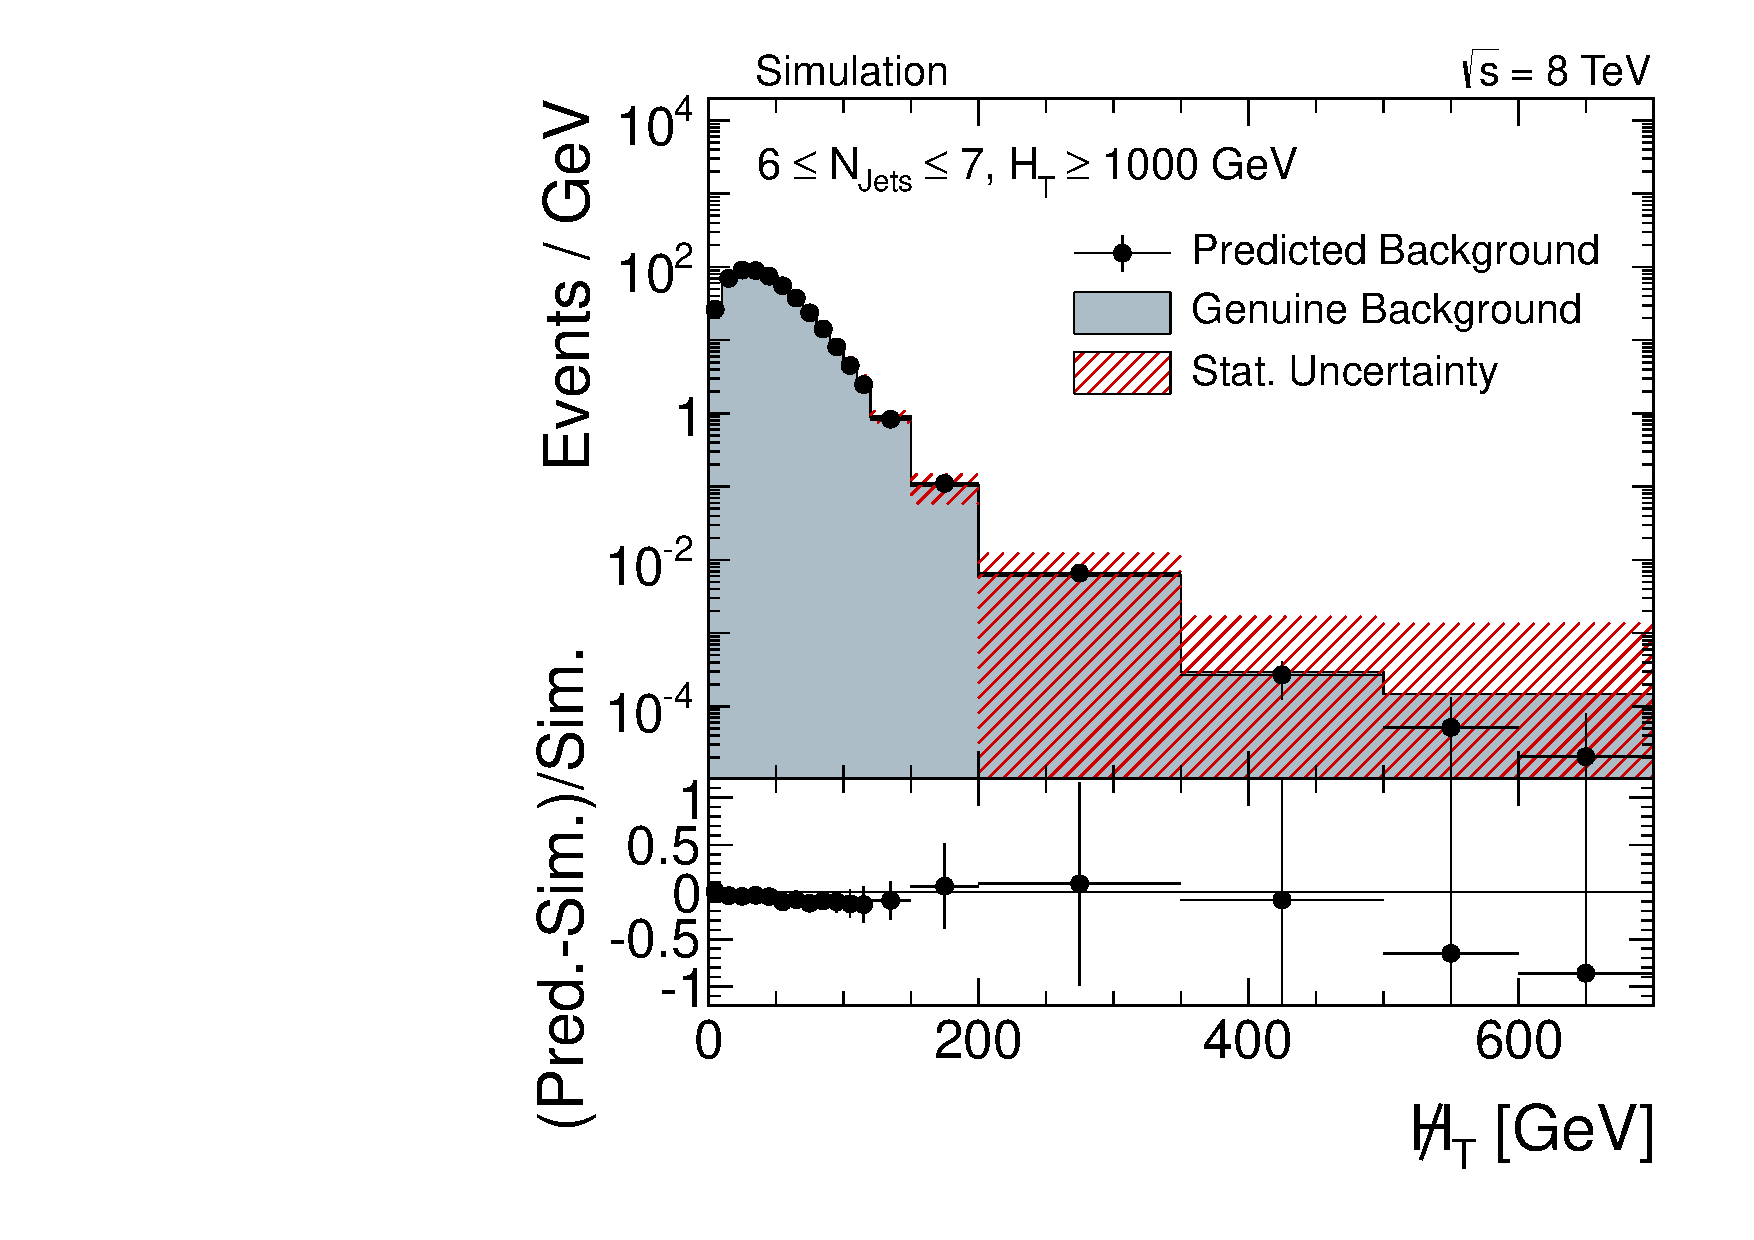
\includegraphics[width=0.49\textwidth]{figures/MHT_JetBin3_HThigh_madgraph_DR53X_chs_TuneZ2star_pt10_withoutPUReweighting_UseRebCorrection_v1.pdf}\\
                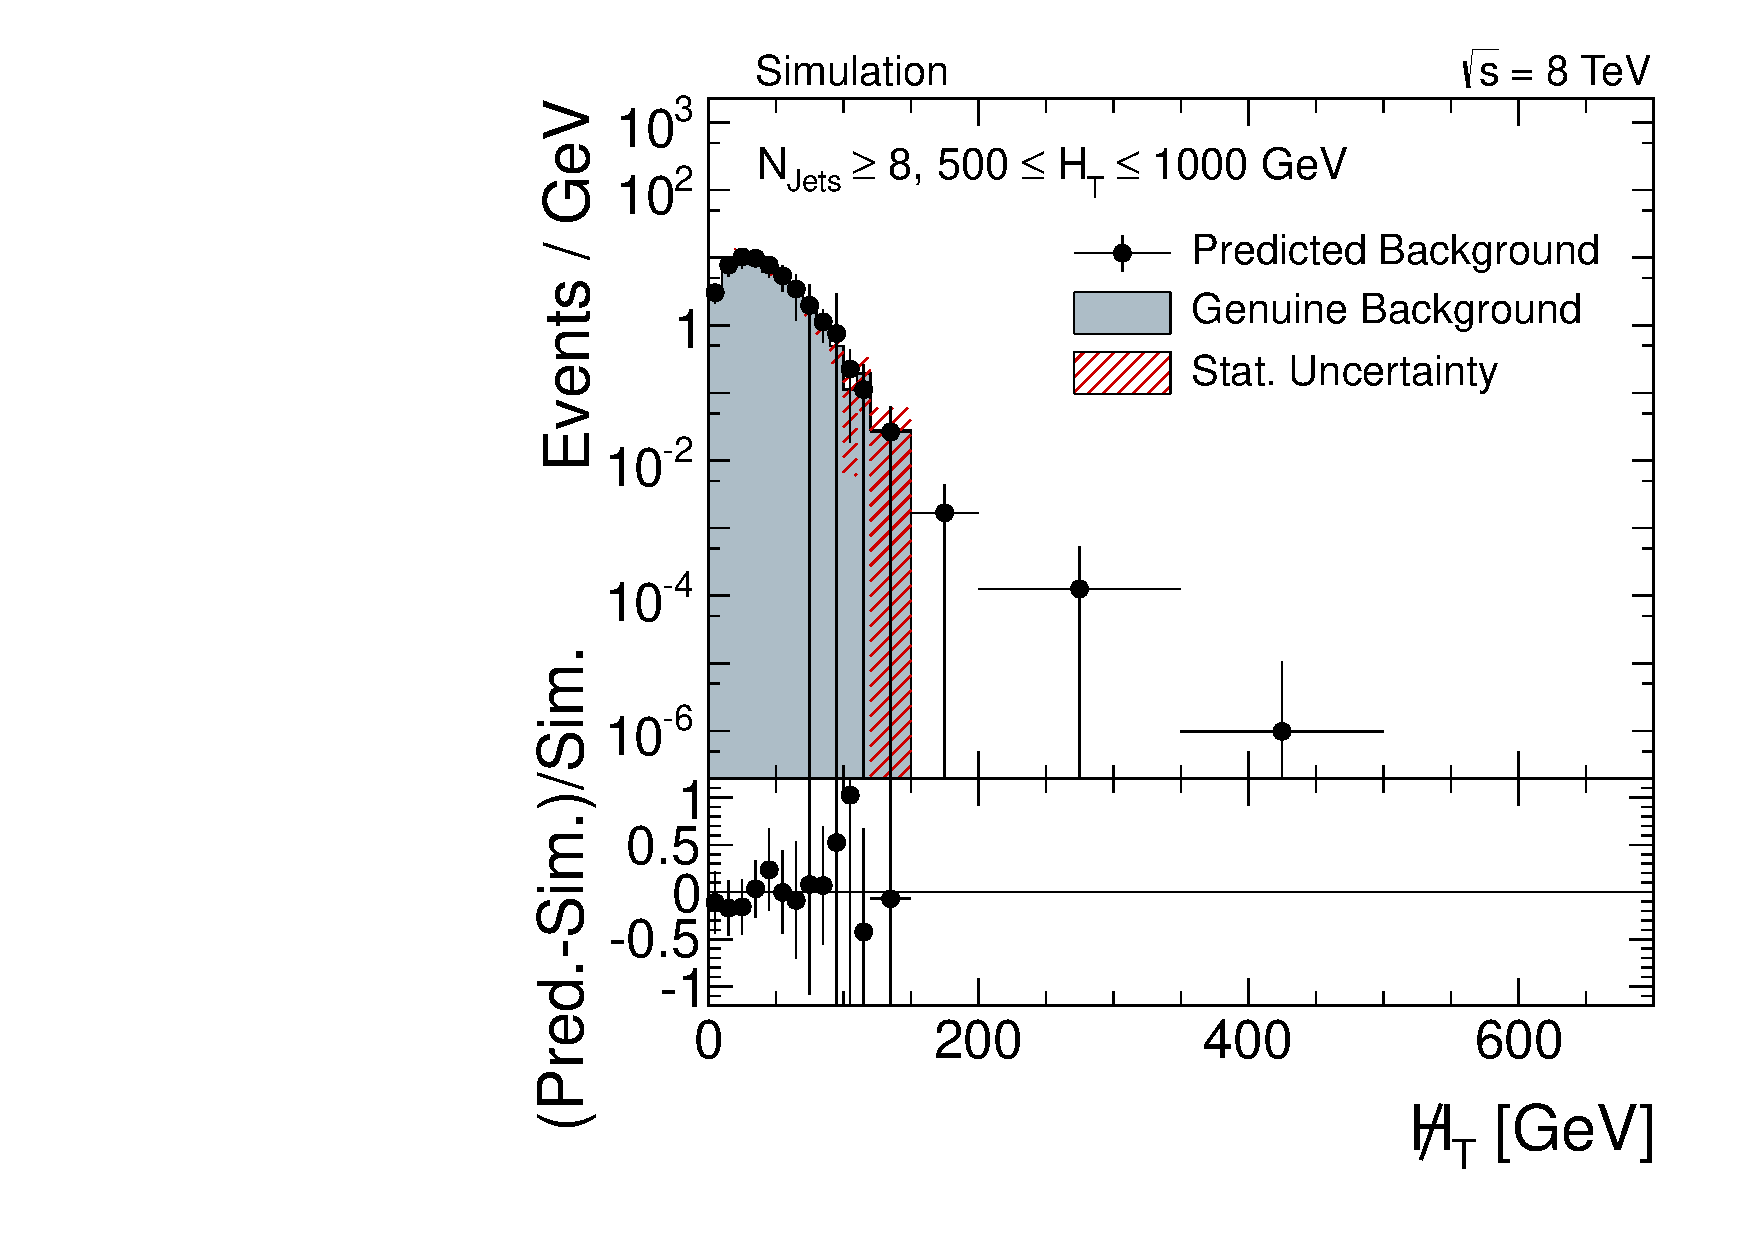
\includegraphics[width=0.49\textwidth]{figures/MHT_JetBin4_HTlow_madgraph_DR53X_chs_TuneZ2star_pt10_withoutPUReweighting_UseRebCorrection_v1.pdf} &
                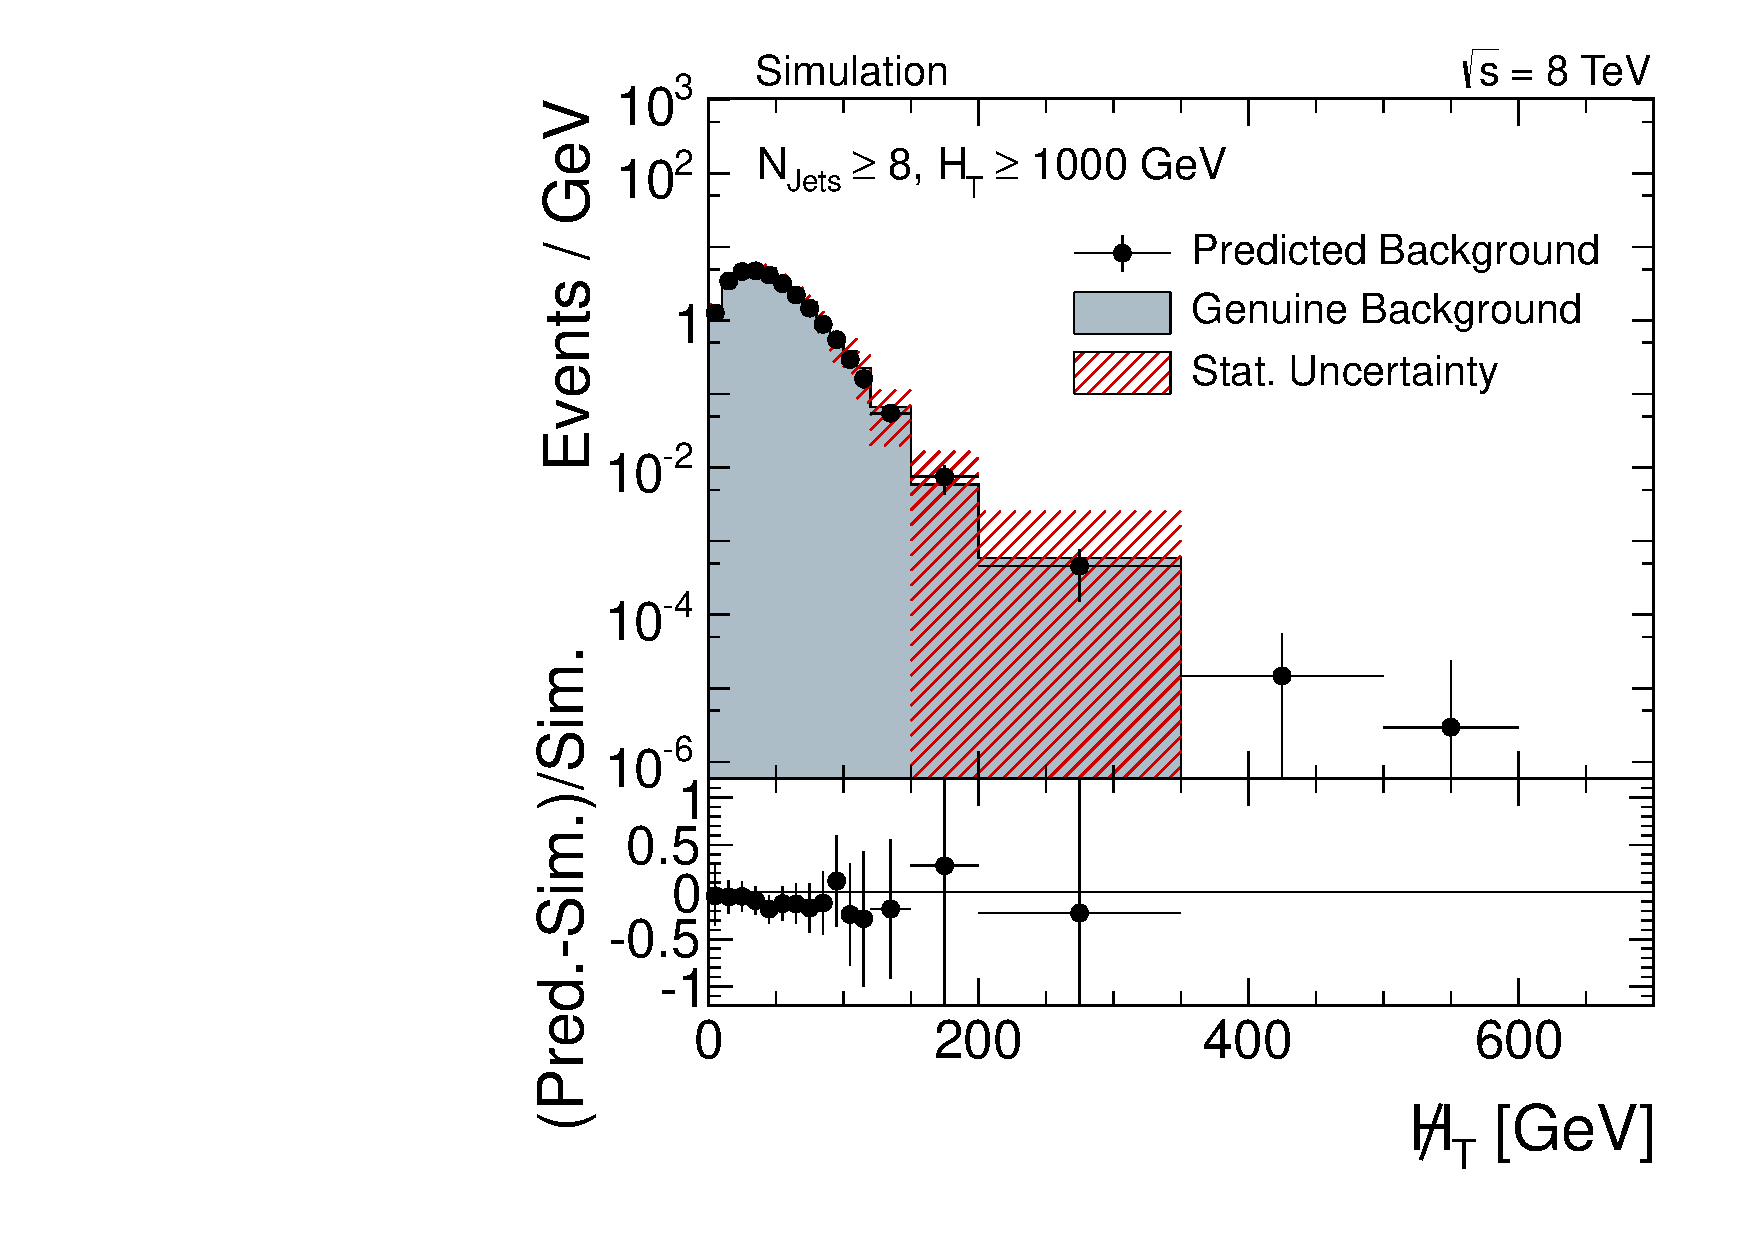
\includegraphics[width=0.49\textwidth]{figures/MHT_JetBin4_HThigh_madgraph_DR53X_chs_TuneZ2star_pt10_withoutPUReweighting_UseRebCorrection_v1.pdf}\\

  \end{tabular}
  \caption{Prediction of QCD background on a QCD multijet sample generated with \madgraph compared to the expectation from full simulation. The closure test is shown for various jet multiplicity bins and low (\textit{left}) or high (\textit{right}) \HT selections.}
  \label{fig:qcd_rs_closure}
\end{figure}
\begin{table}[!t] 
  \centering
  \caption{Summary of non-closure uncertainties with statistical uncertainties derived from the \madgraph QCD sample for the signal region (\textit{first column}) and two control regions which are defined by $100 < \MHT < 200$\gev (\textit{second column}) and inverted $\Delta \phi$ criterion (\textit{third column}). The fourth column is used as additional cross check region, as described in the text. The numbers marked in bold letters are considered as the final non-closure uncertainties of the method.} 
  \label{tab:qcd_rs_closure_unc}
  \resizebox{\textwidth}{!}{%
%   \makebox[\linewidth]{
    \begin{tabular}{cc|cccc} 
      \multicolumn{6}{c}{} \\
      \hline
      & & Signal region & Control region 1 & Control region 2 & Cross check region\\
      \hline
      $N_{\text{jets}}$ & \HT (GeV) & \MHT $>~200$ GeV &  \MHT $= 100 - 200$~GeV  &  \MHT $>~200$ GeV & \MHT $= 100 - 200$~GeV\\
      & & $\Delta \phi$ cut & $\Delta \phi$ cut & $\Delta \phi$ cut inverted & $\Delta \phi$ cut inverted\\
      \hline
      3 -- 5  & 500 -- 1000 & (\textbf{60.4} $\pm$~9.8)\% & (22.6 $\pm$~1.6)\% & (20.1 $\pm$~6.0)\% & (2.8 $\pm$~1.3)\%\\
      6 -- 7  & 500 -- 1000 & (43.1 $\pm$~46.5)\% & (\textbf{25.4} $\pm$~11.1)\% & (59.3 $\pm$~96.0)\% & (4.6 $\pm$~20.0)\%\\
      $\ge$ 8 & 500 -- 1000 & -- & (8.9 $\pm$~90.1)\% & (\textbf{86.0} $\pm$~38.2)\% & (12.2 $\pm$~66.4)\%\\
      \hline
      3 -- 5  & $\ge$ 1000 & (17.1 $\pm$~35.0)\% & (14.4 $\pm$~3.1)\% & (\textbf{14.5} $\pm$~8.9)\% & (5.1 $\pm$~1.7)\%\\
      6 -- 7  & $\ge$ 1000 & (5.5 $\pm$~108.0)\% & (\textbf{10.9} $\pm$~8.8)\% & (14.5 $\pm$~42.9)\% & (3.0 $\pm$~7.0)\%\\
      $\ge$ 8 & $\ge$ 1000 & (19.4 $\pm$~276.0)\% & (21.8 $\pm$~28.6)\% & (40.4 $\pm$~293.5)\% & (21.1 $\pm$~\textbf{42.6})\%\\
      \hline
    \end{tabular}}
\end{table}
\\
The first choice for the determination of remaining biases is to calculate for the signal region, defined by \MHT $>$~200 GeV and the application of the $\Delta \phi$ cut, the relative difference between prediction and expectation normalized to the expectation. Then, this relative difference can be considered as systematic uncertainty. In case it is statistically significant within $\pm 1\sigma$ uncertainty, the prediction could also be corrected for the non-closure. The calculated relative differences with their statistical uncertainties are summarized in Tab.~\ref{tab:qcd_rs_closure_unc} (first column) for the signal region. The table shows that there is one bin ($3 \leq \NJets \leq 5$ and $500 \leq \HT \leq 1000$\gev) in which the signal region shows a statistically significant non-closure. In Fig.~\ref{fig:qcd_rs_closure_comp}, this particular distribution is shown for the \madgraph QCD sample (left) and alternatively for a QCD sample generated with \pythia (right), as used for the studies in Chap.~\ref{chap:Resolution}. In the region for $200 < \MHT < 350$\gev, the \madgraph sample exhibits an underprediction of $\approx 60\%$, while the \pythia sample tends to a statistically non-significant overprediction. Thus, it is difficult to judge, if the observed underprediction in the test performed with \madgraph is a systematic effect or just a statistical fluctuation. In order to treat this observed difference conservatively, the predicted result is not corrected for this potential deviation, but the total 60\% deviation observed in the \madgraph sample is considered as systematic uncertainty. Since QCD is not the dominant background contribution in the search regions defined by $3 \leq \NJets \leq 5$ and $500 \leq \HT \leq 1000$\gev, this rather large uncertainty has hardly an impact on the final result of the analysis.
\begin{figure}[!t]
  \centering
  \begin{tabular}{cc}
                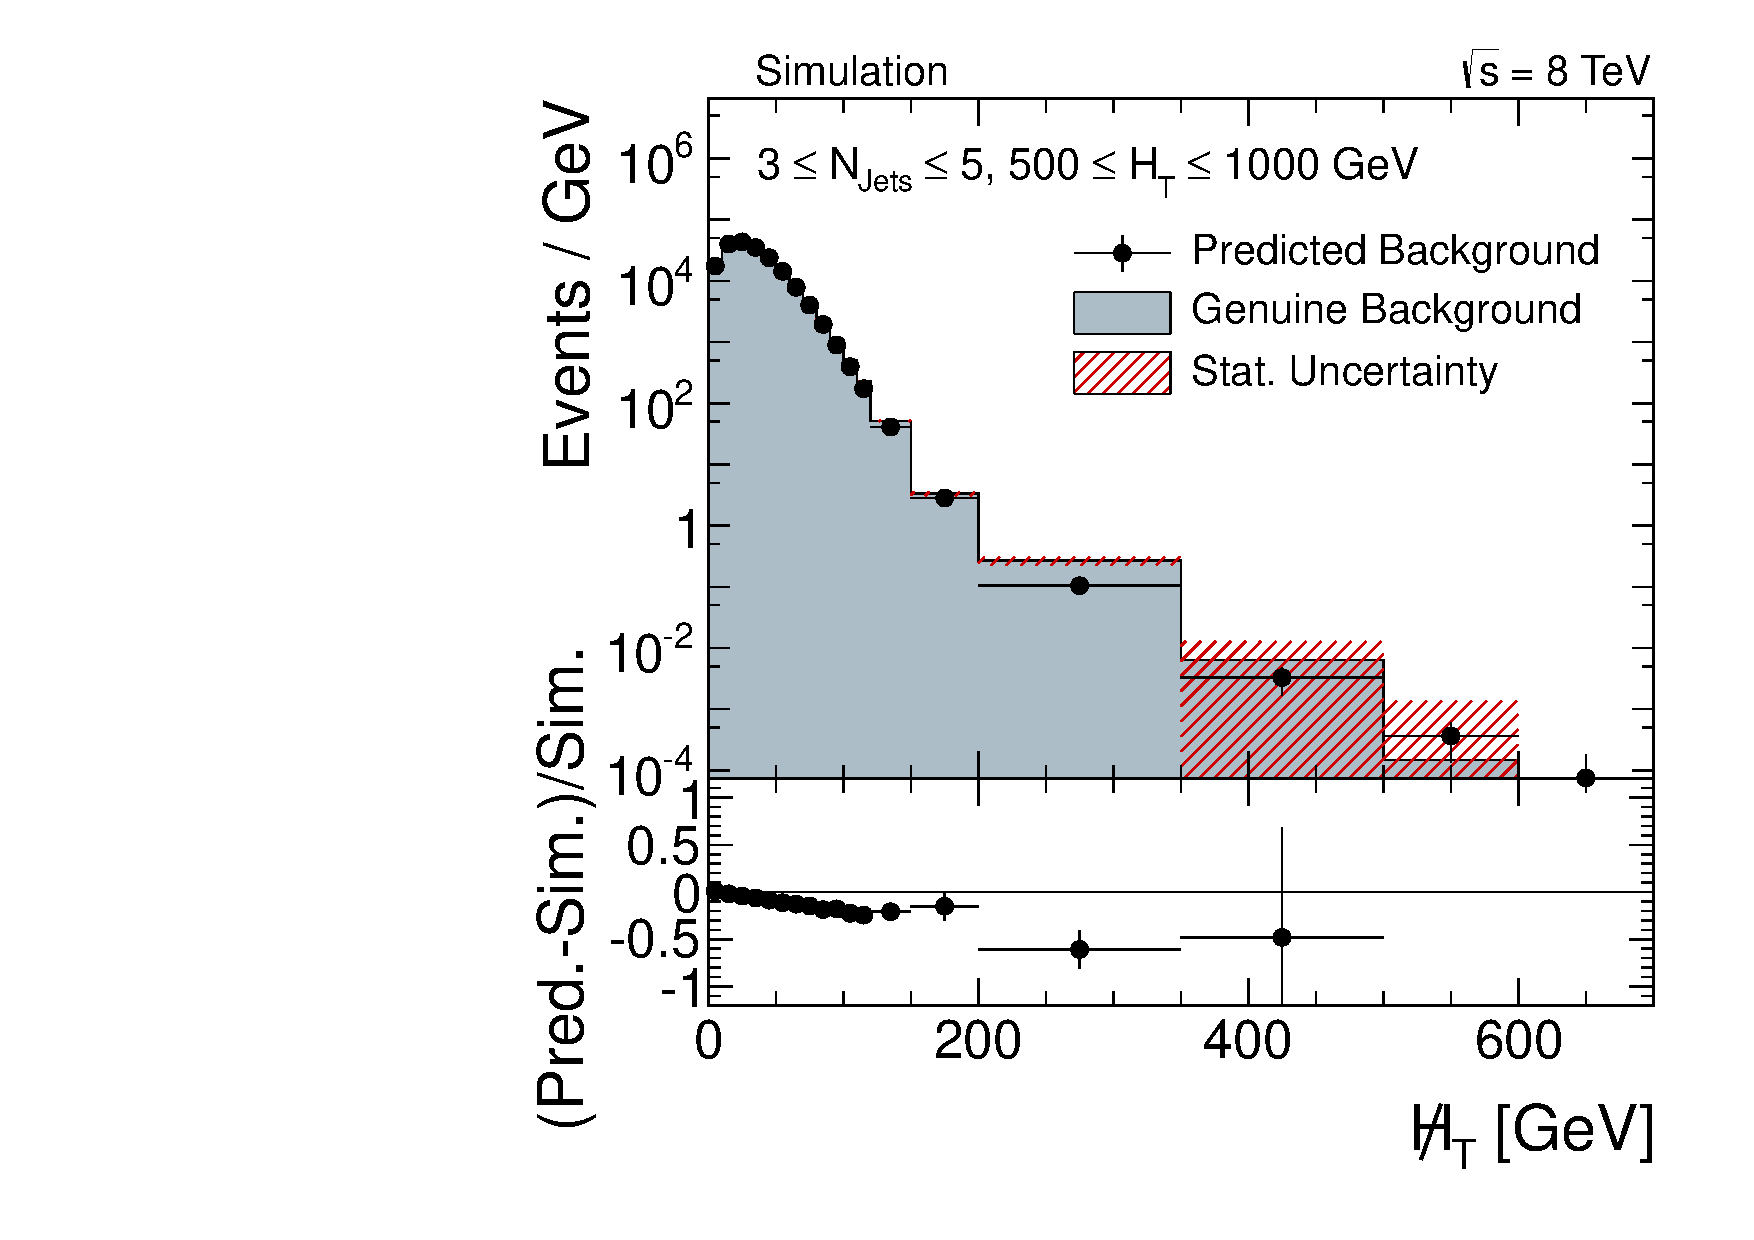
\includegraphics[width=0.49\textwidth]{figures/MHT_JetBin2_HTlow_madgraph_DR53X_chs_TuneZ2star_pt10_withoutPUReweighting_UseRebCorrection_v1.pdf} &
                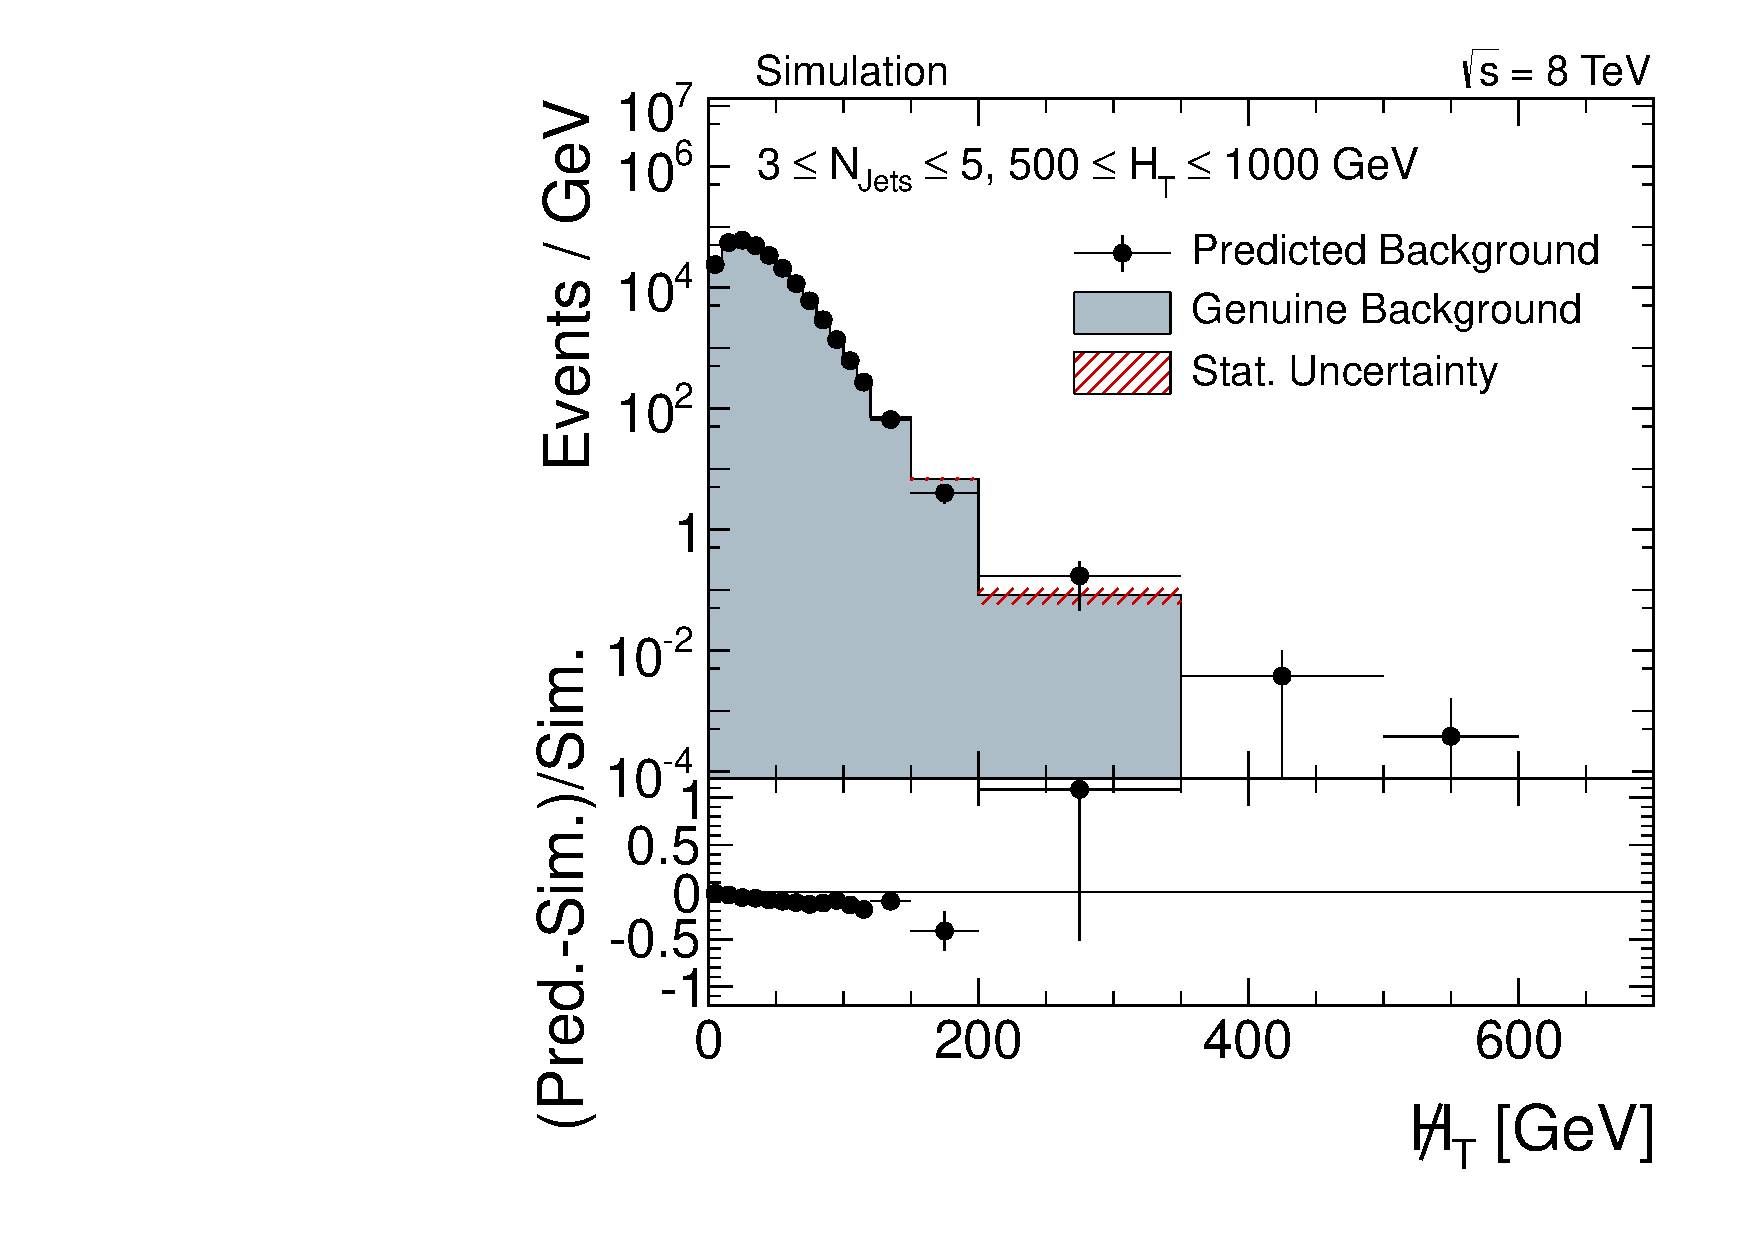
\includegraphics[width=0.49\textwidth]{figures/MHT_JetBin2_HTlow_pythia_DR53X_chs_TuneZ2star_pt10_withoutPUReweighting_UseRebCorrection_v1.pdf}\\
  \end{tabular}
  \caption{Prediction of QCD background on a simulated QCD multijet sample compared to the expectation from full simulation. The closure test is shown for 3--5 jets and $ 500 \leq \HT \leq 1000$~GeV obtained from the \madgraph QCD sample (\textit{left}) and alternatively from a \pythia QCD sample (\textit{right}).}
  \label{fig:qcd_rs_closure_comp}
\end{figure}
\\
Since the number of events in the signal region with $\MHT \ge 200$\gev is low for all bins except for the one discussed above, the respective statistical uncertainties are large. Hence, these bins do not allow reasonable conclusions concerning the closure of the method. Thus, also two sidebands of the signal region are studied and the prediction is compared to the full simulation either for control region 1 defined by $ 100 \leq \MHT \leq 200$\gev (second column in Tab.~\ref{tab:qcd_rs_closure_unc}) or for control region 2 defined by an inverted $\Delta \phi$ criterion (third column in Tab.~\ref{tab:qcd_rs_closure_unc}). The evaluation of the remaining bias aiming at a conservative treatment, proceeds as follows: 
\begin{itemize}
 \item If the differences in both control regions are statistically significant, the larger one is considered as systematic uncertainty. 
 \item If only one of the two numbers in the control regions is statistically significant, it has to be made sure that the assigned uncertainty by taking this number, \eg coming from control region 1, is not too small, as a remaining bias might come from the application of the $\Delta \phi$ cut. Thus, the value is compared to the value and its uncertainty in the corresponding cross check region bin (right column of Tab.~\ref{tab:qcd_rs_closure_unc}). If the value and its uncertainty in the cross check region are smaller than the chosen value from the control region, the number from the control region is considered as systematic error. Otherwise take largest number from cross check region (deviation or its uncertainty).
 \item If none of the numbers in the control regions is statistically significant, take the number with higher precision and proceed as above by comparing this value to the numbers in the cross check region. If the cross check region does not show larger values, take the number with highest precision, otherwise take largest number from cross check region.
\end{itemize}
The uncertainty which is finally considered by the procedure described above as the uncertainty quantifying the remaining bias of the R+S method, is printed in bold letters in Tab.~\ref{tab:qcd_rs_closure_unc}.

\subsection{Application to Data Events}
\label{subsec:validation_data_R+S}
\begin{figure}[!t]
  \centering
  \begin{tabular}{cc}
                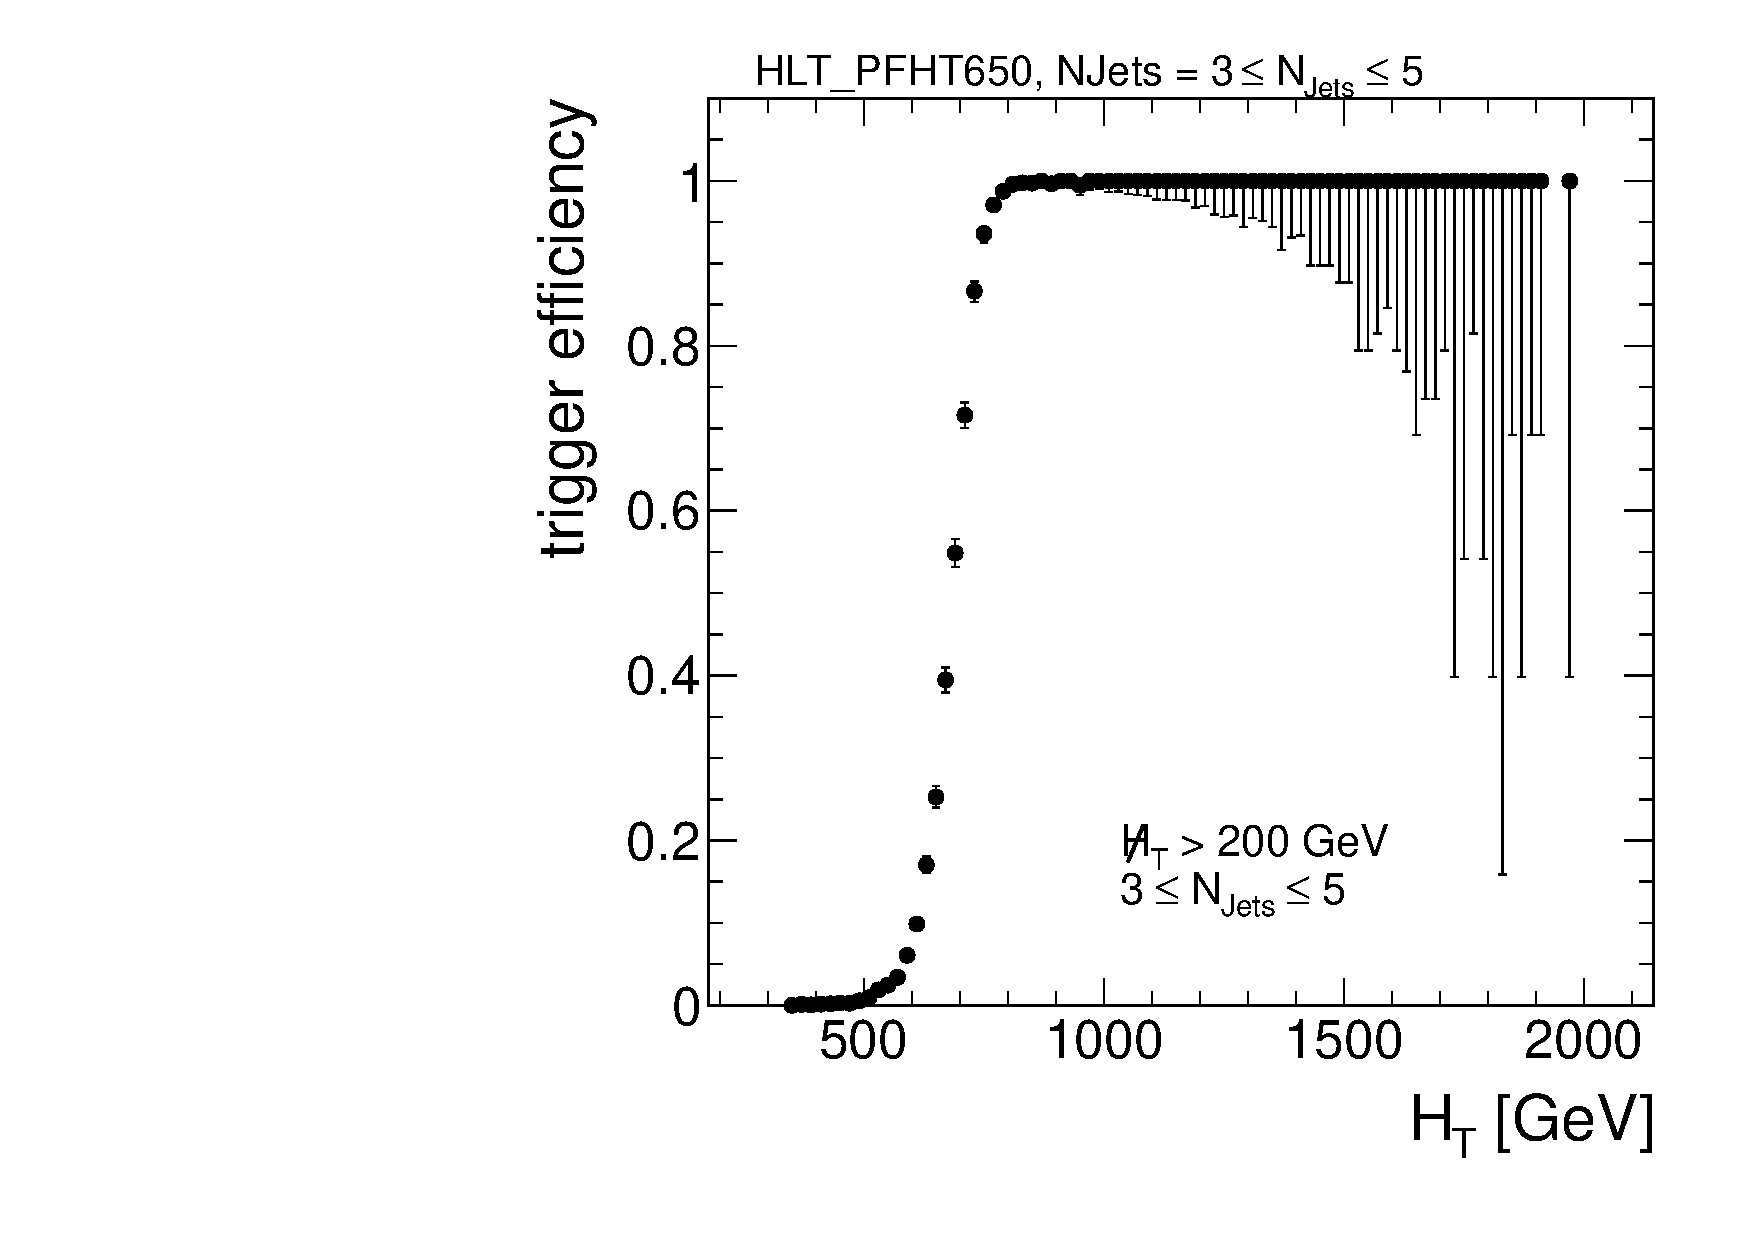
\includegraphics[width=0.49\textwidth]{figures/turn_on_HT_TagEle27WP80_ProbePFHT650_chs_NJets3-5.pdf} &
                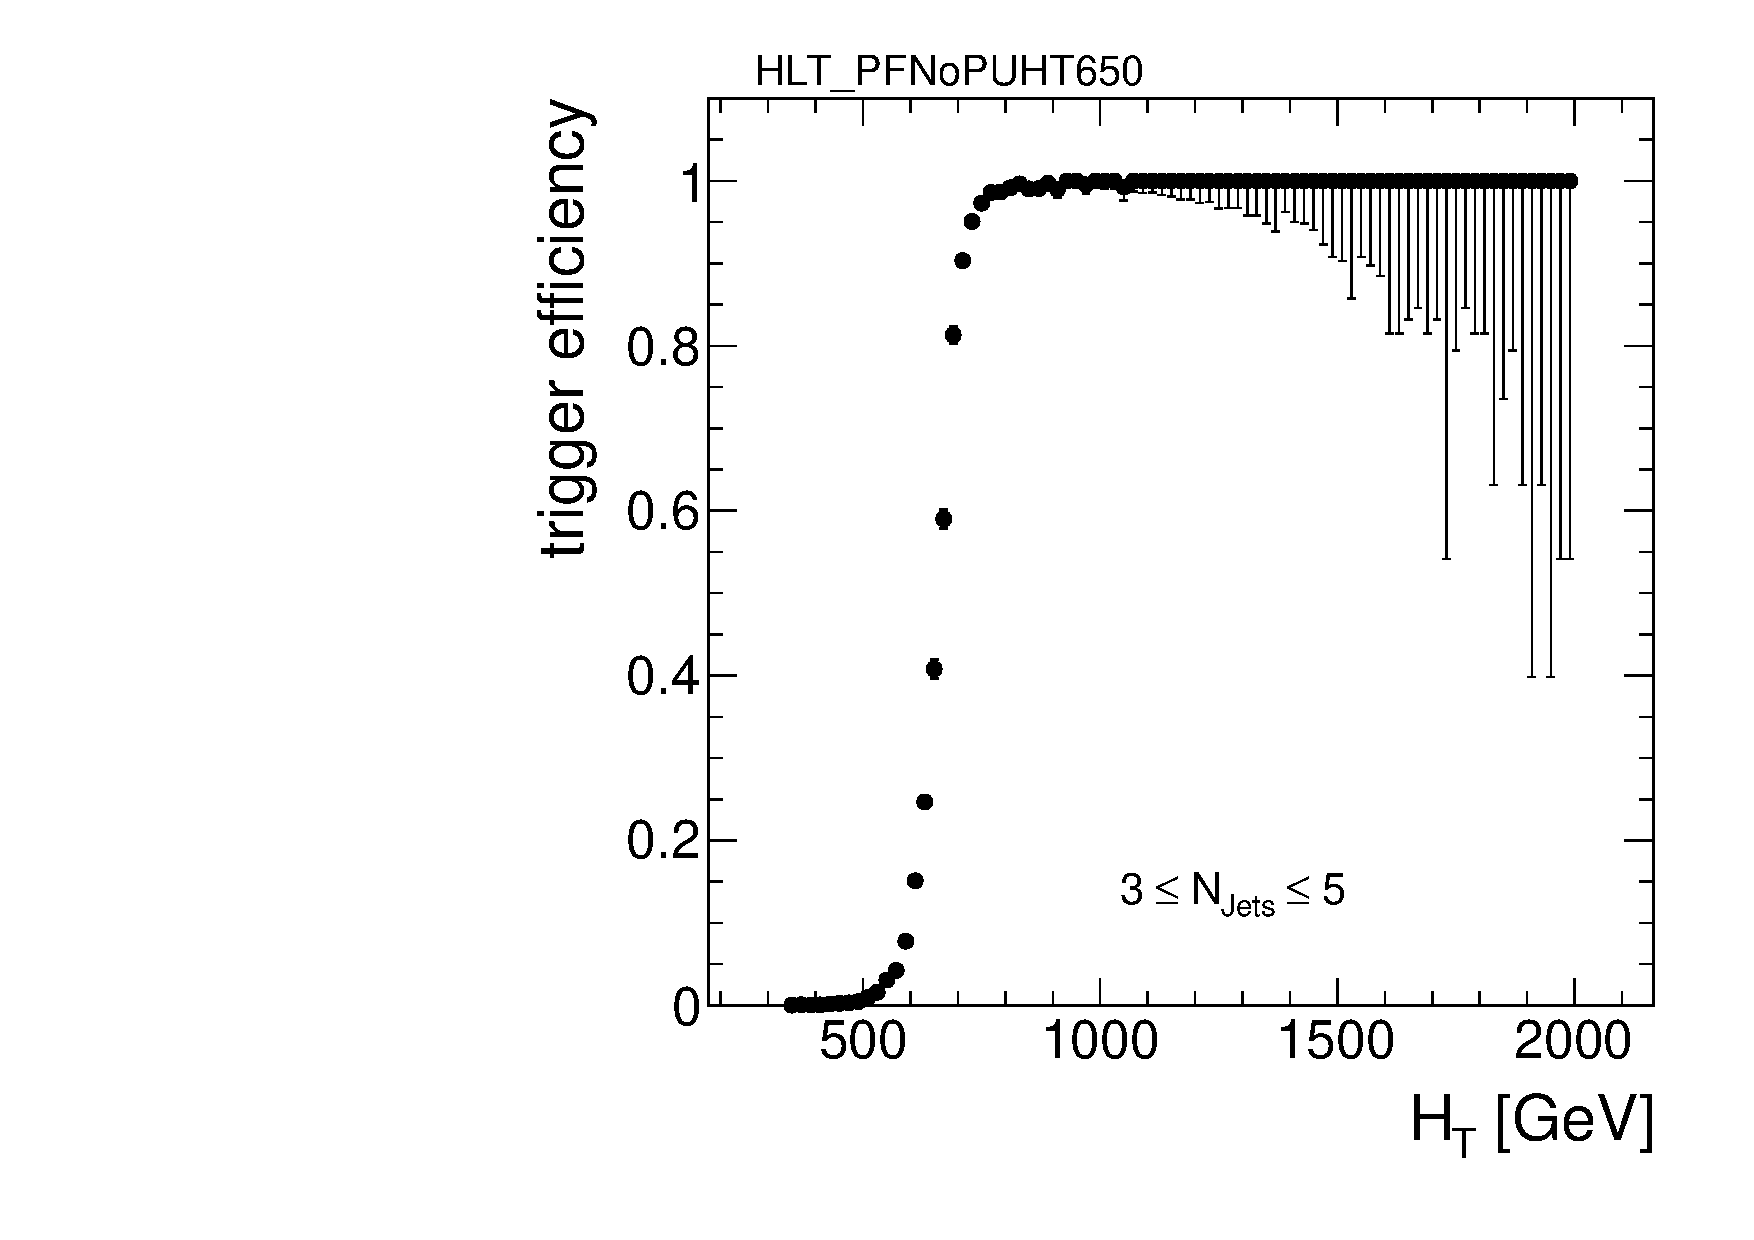
\includegraphics[width=0.49\textwidth]{figures/turn_on_HT_TagEle27WP80_ProbePFNoPUHT650_chs_NJets3-5.pdf} \\
  \end{tabular}
\caption{Measured trigger efficiency for paths HLT\_PFHT650 (\textit{left}) and HLT\_PFNoPUHT650 (\textit{right}) as a function of \HT, shown for $3 \leq$ \NJets $\leq 5$.} 
  \label{fig:trig_eff_650_3njets5}
\end{figure}
After the successful validation of the R+S method in simulated events and a quantification of a possible remaining bias, the procedure can finally be applied to data, in order to estimate the QCD background contributions. \\
The QCD background prediction is performed on a QCD multijet data control sample. This is collected by two triggers based on \HT calculated from PF jets. The nominal \HT thresholds of the two triggers are 350\gev and 650\gev, respectively. The trigger efficiency as a function of \HT for a nominal threshold of 350\gev has been evaluated already for the signal trigger in Sec.~\ref{subsec:RA2_samples_trigger} and was observed to be fully efficient for the baseline \HT cut. The trigger efficiencies for the respective trigger with $\HT = 650$\gev are shown in Fig.~\ref{fig:trig_eff_650_3njets5} for a jet multiplicity of 3--5 and for jet multiplicities $6 \leq \NJets \leq 7$ and $\NJets \geq 8$ in App.~\ref{fig:trig_eff_650_6njets7} and App.~\ref{fig:trig_eff_650_njets8}, respectively. For these jet multiplicities, the trigger paths are fully efficient for a \HT selection of 800\gev. Since two different \HT threshold triggers are used, each event of the multijet control sample has to be unambigously assigned to one trigger to avoid double-counting of certain events and to gain a smooth \HT spectrum which allows an unbiased background prediction. Taking into account that the trigger with the lower \HT threshold has been prescaled during operation, this is done as follows: For each event, the trigger which fired and has the lowest prescale factor is determined. Then the event is weighted according to the prescale factor. Since only one prescaled and one unprescaled trigger is considered, this assignment is unambigious and leads to a smooth \HT spectrum which starts at the lowest trigger threshold. The prescale weighted seed \HT distribution is illustrated in Fig.~\ref{fig:qcd_rs_seedht}.
\begin{figure}[!t]
  \centering
  \begin{tabular}{c}
                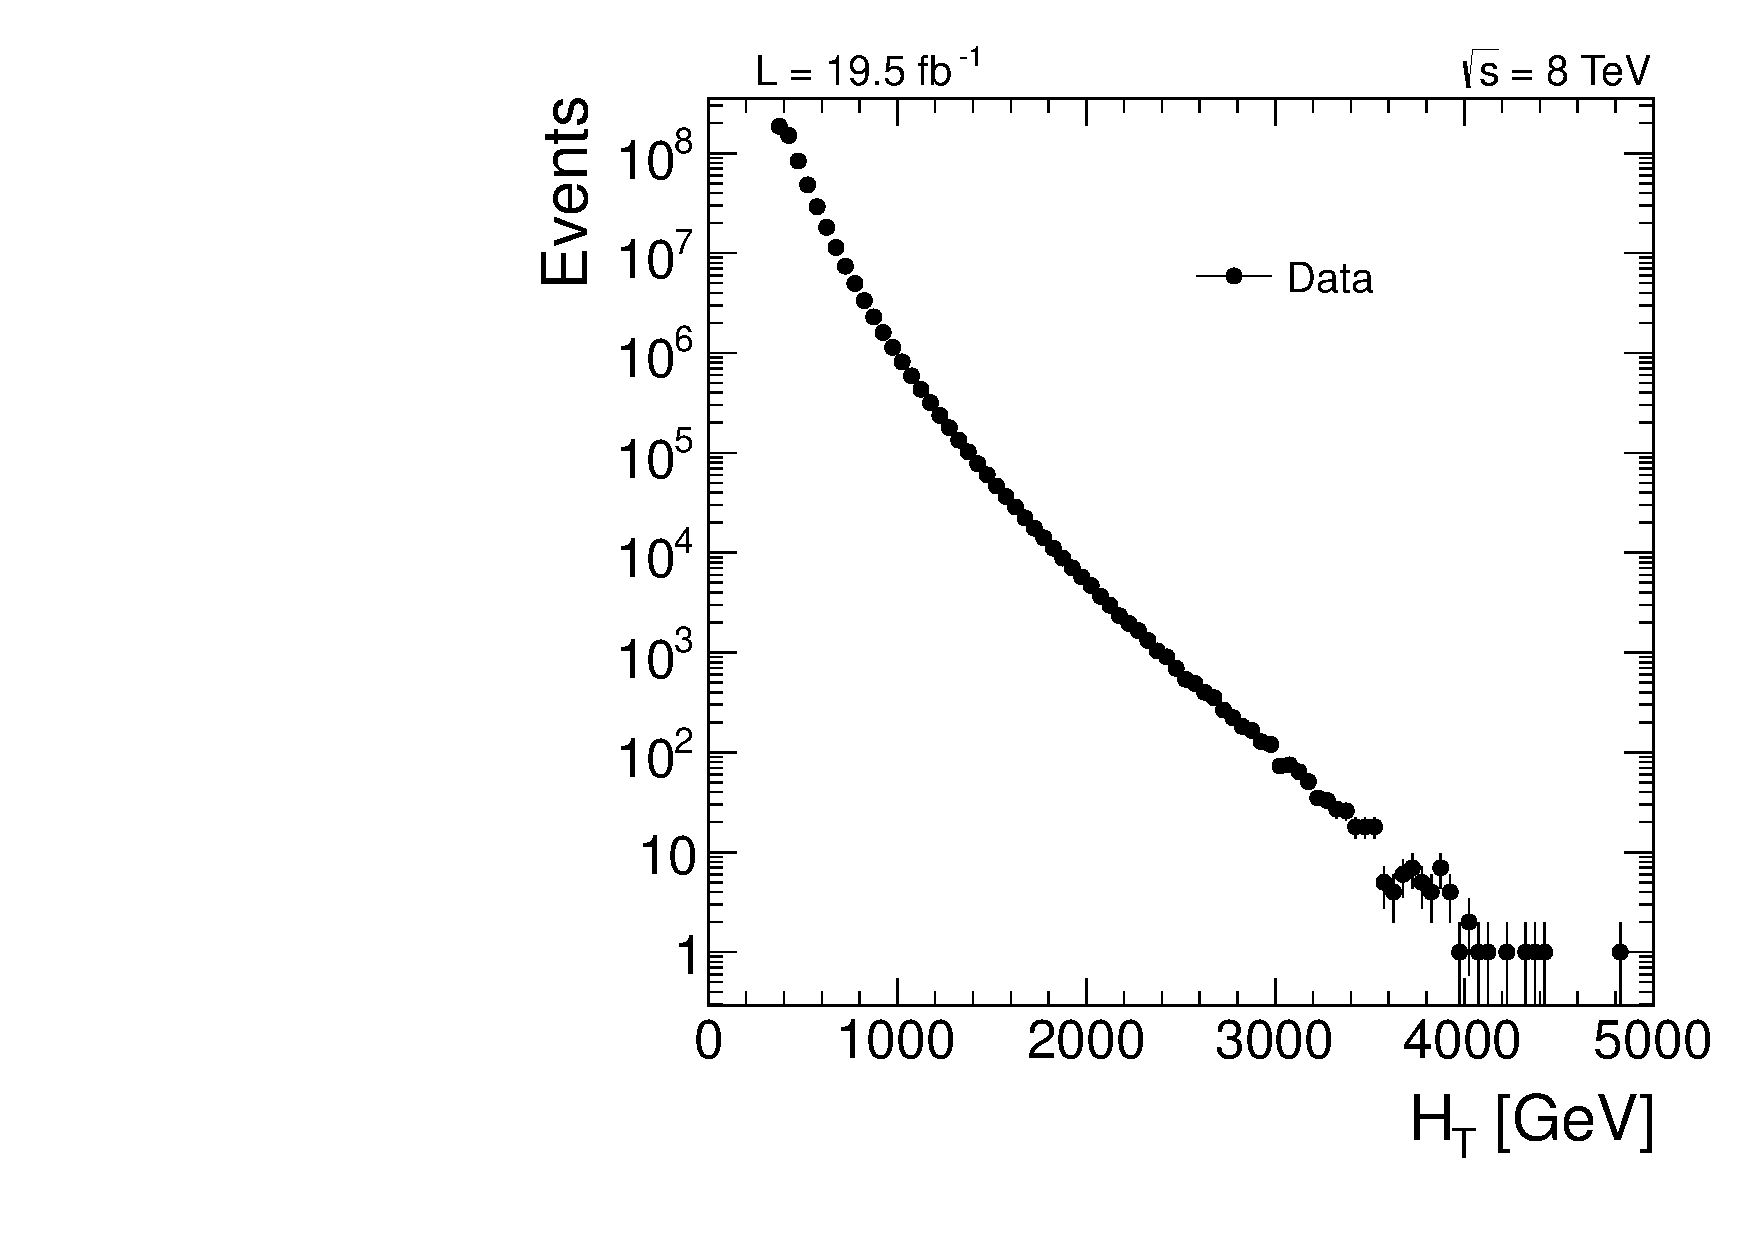
\includegraphics[width=0.49\textwidth]{figures/HT_data.pdf}
  \end{tabular}
  \caption{Seed \HT spectrum of full 2012 dataset used as input for the R+S method after correcting for trigger prescales.}
  \label{fig:qcd_rs_seedht}
\end{figure}
The usage of the prescaled trigger is necessary, in order to collect also events with $\HT < 800$\gev and in particular also events with \HT values below the minimum \HT threshold of the signal region. The latter events have to be considered, since they can pass $\HT > 500$\gev through a fluctuation to large response values. However, the events collected by the prescaled trigger have high event weights and spoil artificially the prediction when they enter the signal region, as they lead to a substantially higher uncertainty. As described for the hadronic-tau background, this is solved by smearing the events obtained from the prescaled trigger not only once but $M$ times (with $M =$ prescale factor), and weighting them accordingly with one.

\subsection{Validation in Data Events}
Similar to the validation in simulated events, also the application of the R+S method to data can be validated. This is done by comparing the prediction of the R+S method from data to selected events in a QCD enriched data control sample. \\
The control sample is defined by at least three jets, $\HT > 1000$\gev, an inverted $\Delta \phi$ criterion and $100 \leq \MHT \leq 200$\gev. The resulting comparison between predicted QCD multijet background events obtained from the R+S method and selected data events in the control region is shown in Fig.~\ref{fig:qcd_rs_dataclosure} and exhibits reasonable agreement within 10--20\%. This also justifies the approach to consider the correction factor for the rebalancing derived from simulation for data events as well. In general, no perfect agreement is expected in this test, since contaminations from other backgrounds are still present in the data control sample. This is illustrated in the lower row of Fig.~\ref{fig:qcd_rs_dataclosure} in which the background composition is studied in simulated events. The ratios in the bottom display the comparison of the QCD background to the total background and thus provide an estimate for the purity of the control sample. The ratios exhibit a similar trend as seen in the upper row for the comparison of the QCD prediction to the data control sample and confirm that the deviations observed in the data closure-test can essentially be attributed to the contamination of the control region by other backgrounds. The residual contribution of non-QCD background to the chosen QCD control region amounts to 5\% in total and is primarily present for \HT values up to 1500\gev and high jet multiplicities. Deviations observed in the data closure test beyond the contamination of the control sample from other backgrounds are covered by the bias uncertainty studied in Sec.~\ref{subsec:validation_mc}. \\
Overall, the application of the R+S method to predict the QCD background contributions in data is expected to provide reliable results, since the validation tests in simulation as well as in data have a positive outcome. However, systematic uncertainties that have to be considered for the prediction of QCD background are discussed in the next section. 
\begin{figure}[!t]
  \centering
  \begin{tabular}{cc}
                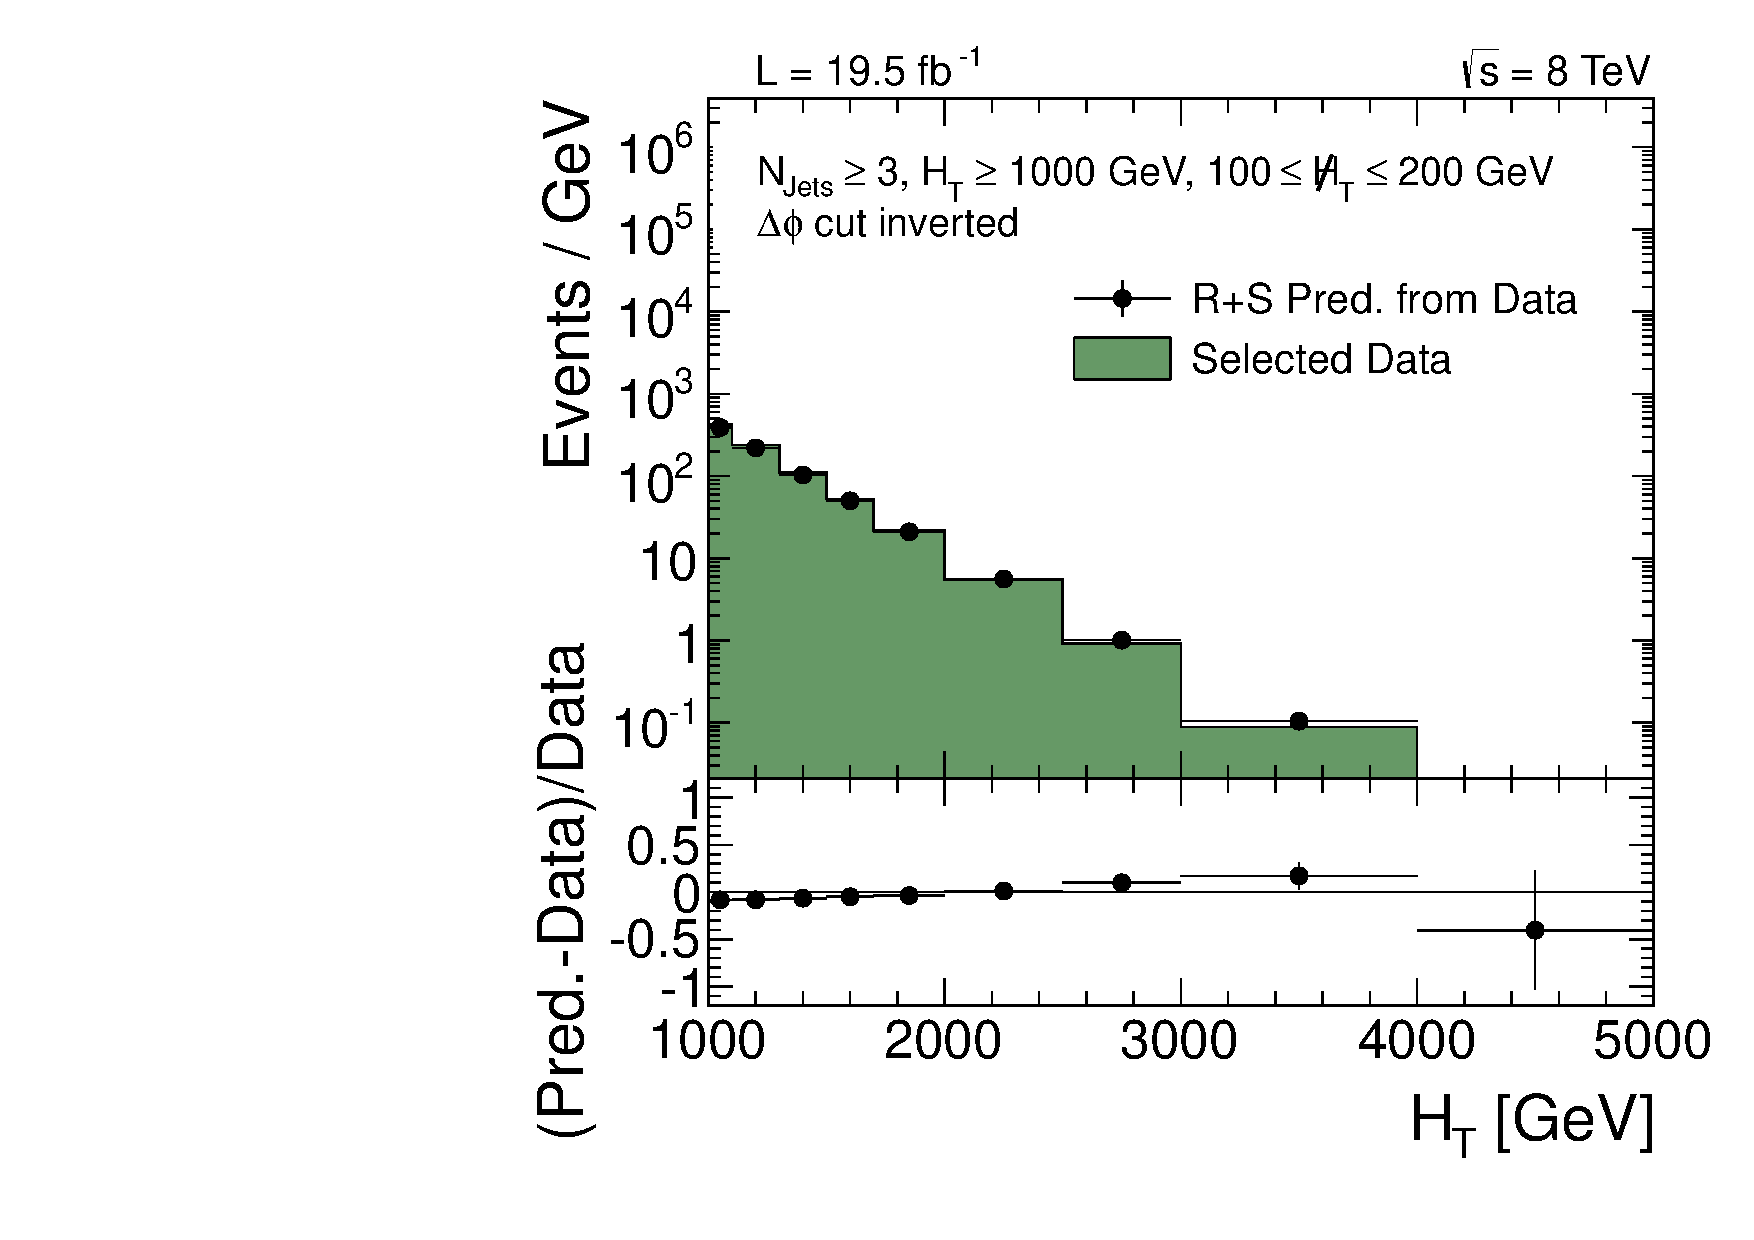
\includegraphics[width=0.49\textwidth]{figures/HT_presel_HThigh_data_DR53X_chs_HThigh_invertedDeltaPhi_v1.pdf} &
                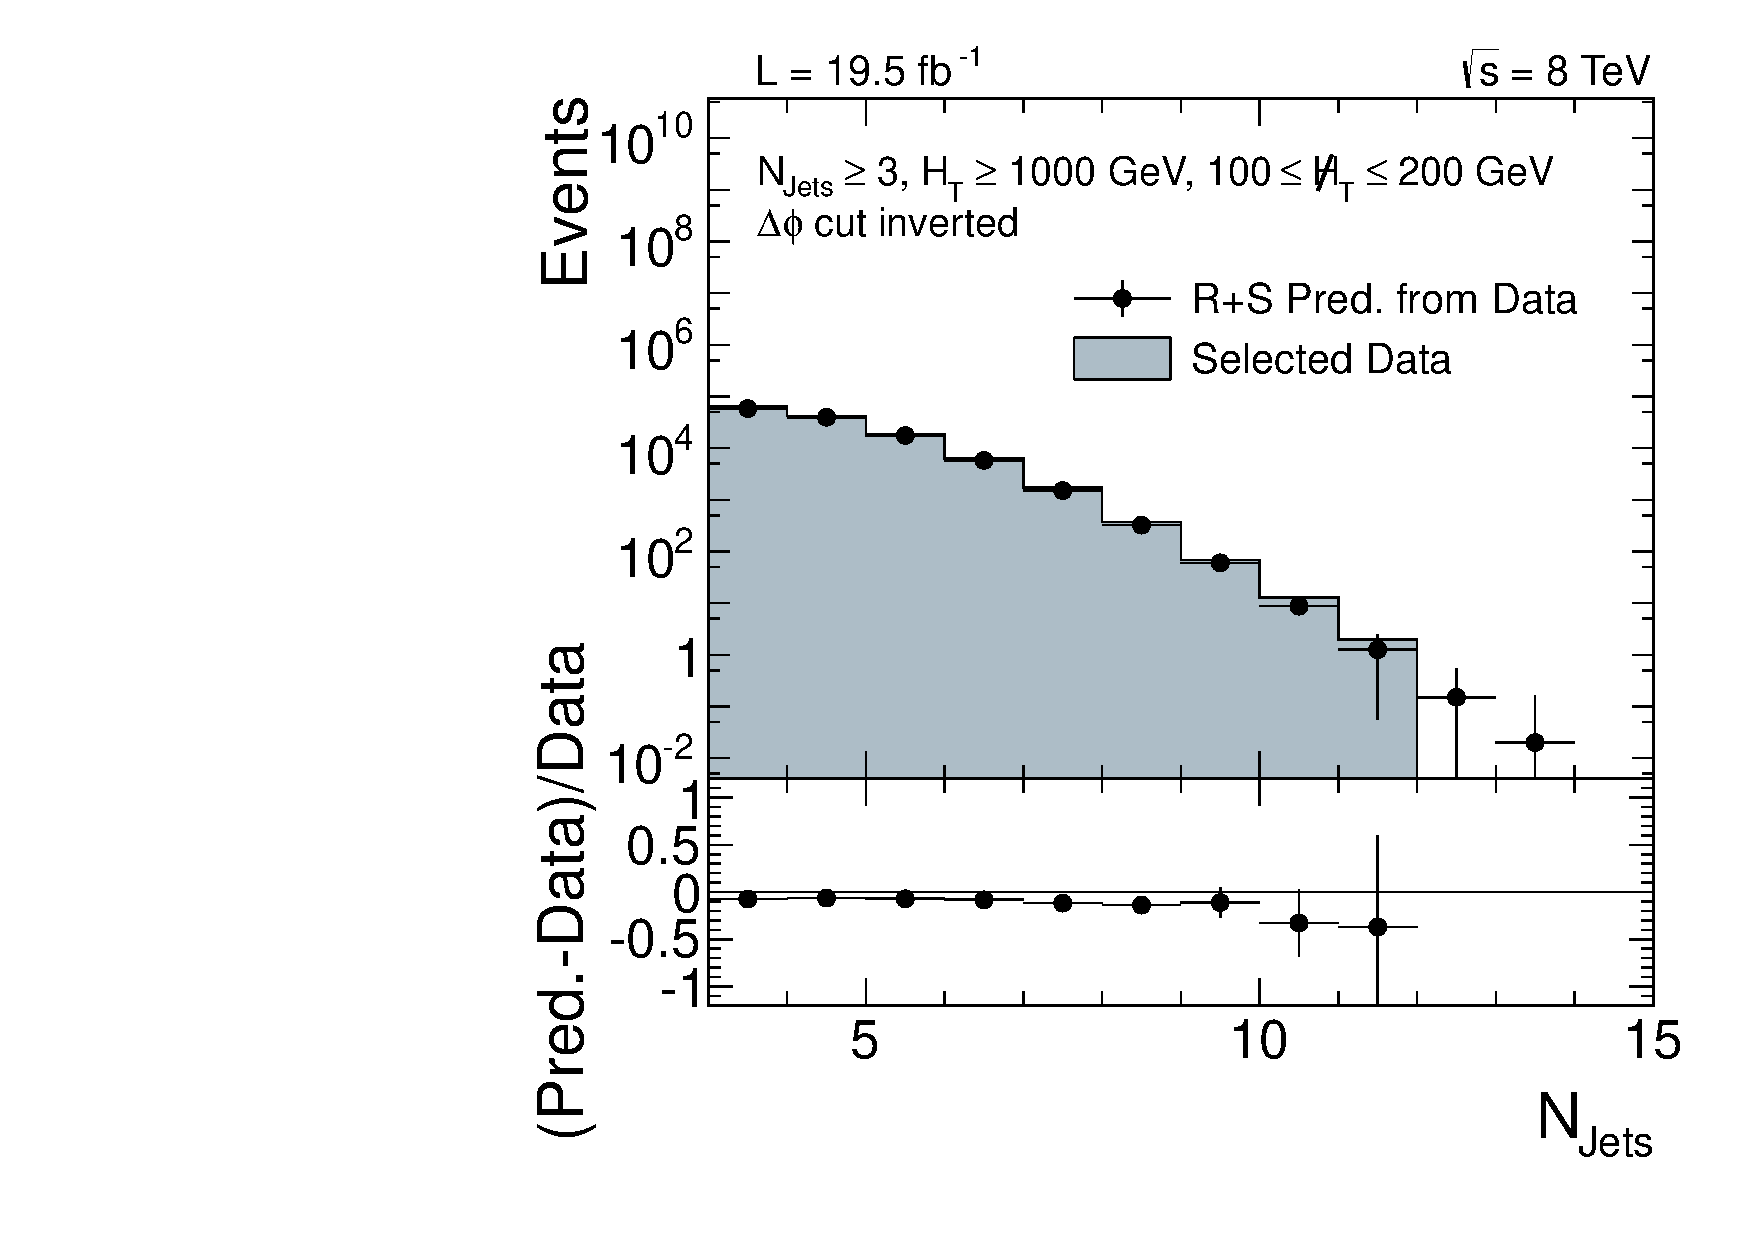
\includegraphics[width=0.49\textwidth]{figures/NJets_presel_HThigh_data_DR53X_chs_HThigh_invertedDeltaPhi_v1.pdf} \\
                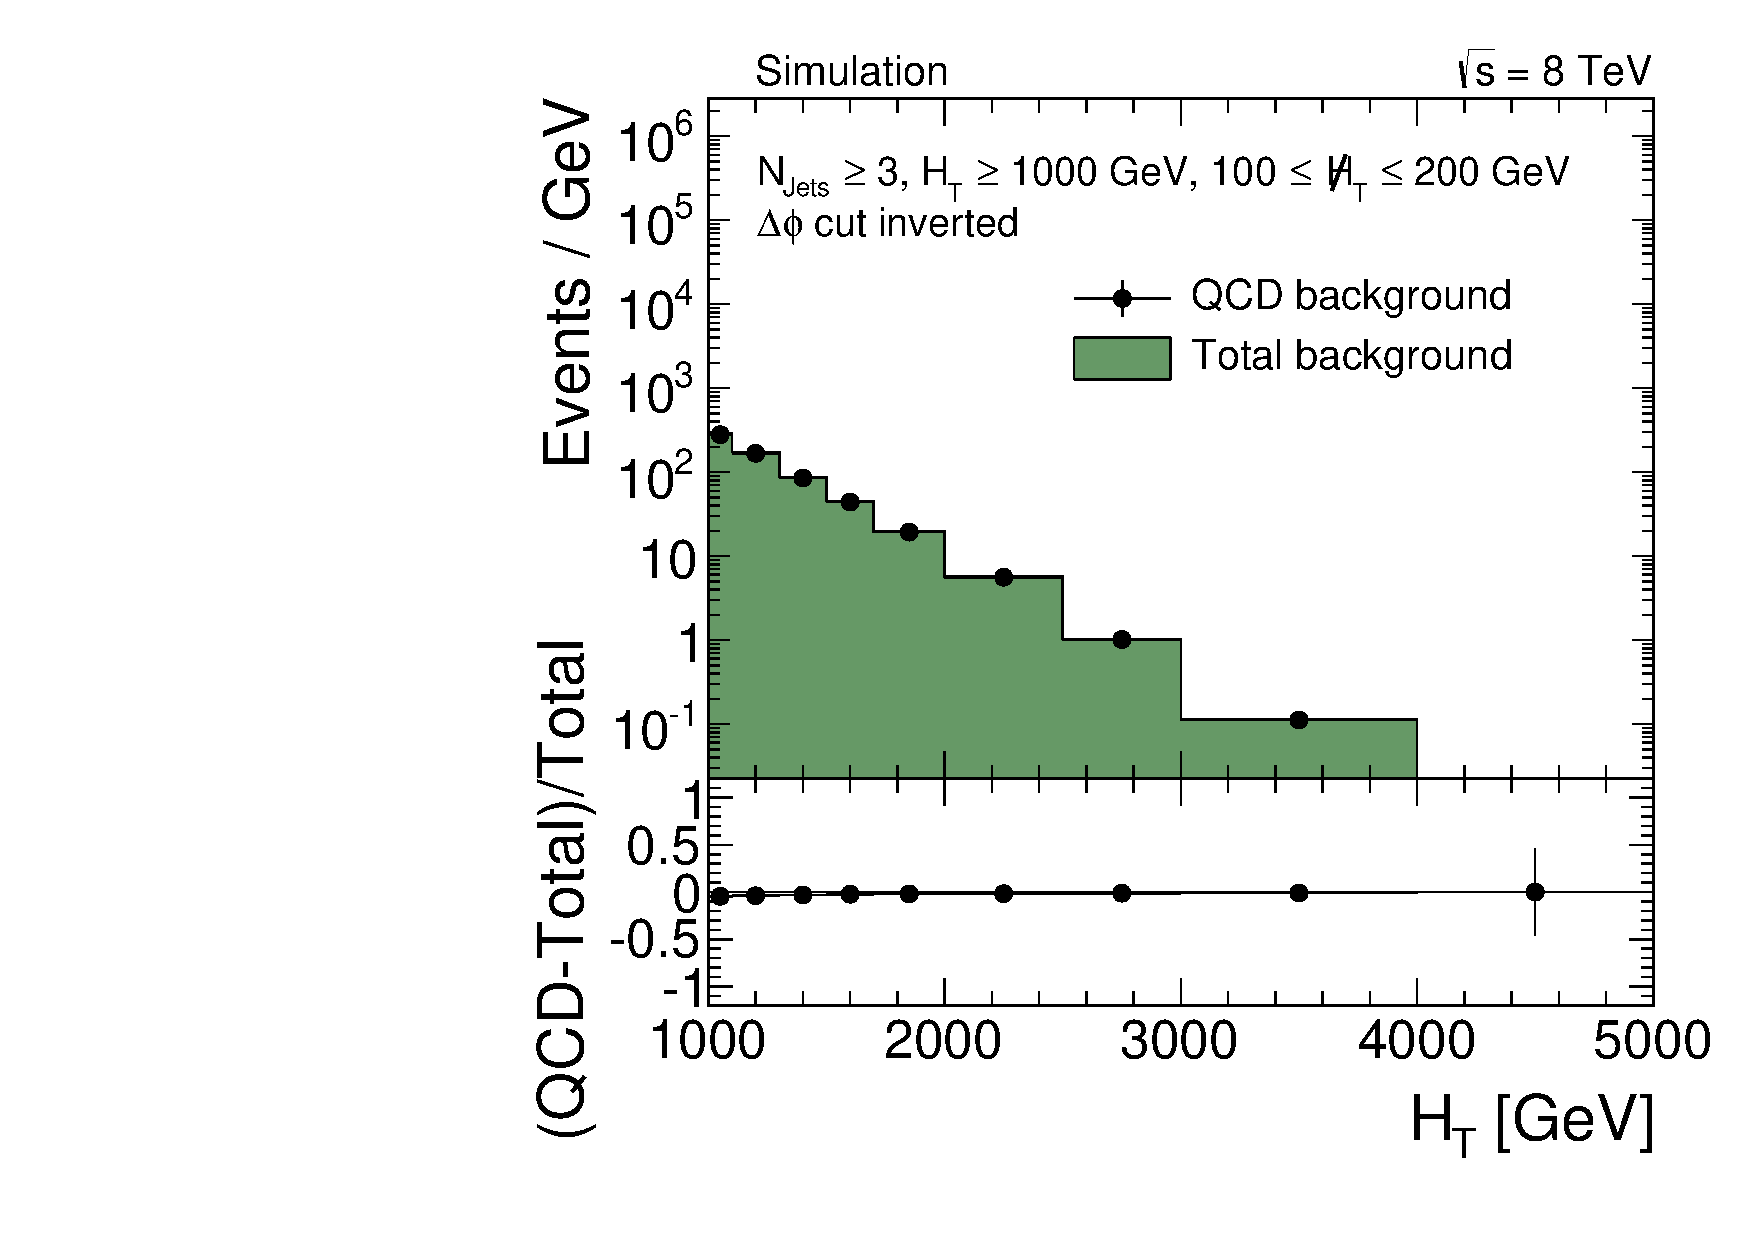
\includegraphics[width=0.49\textwidth]{figures/HTRA2_MC.pdf} &
                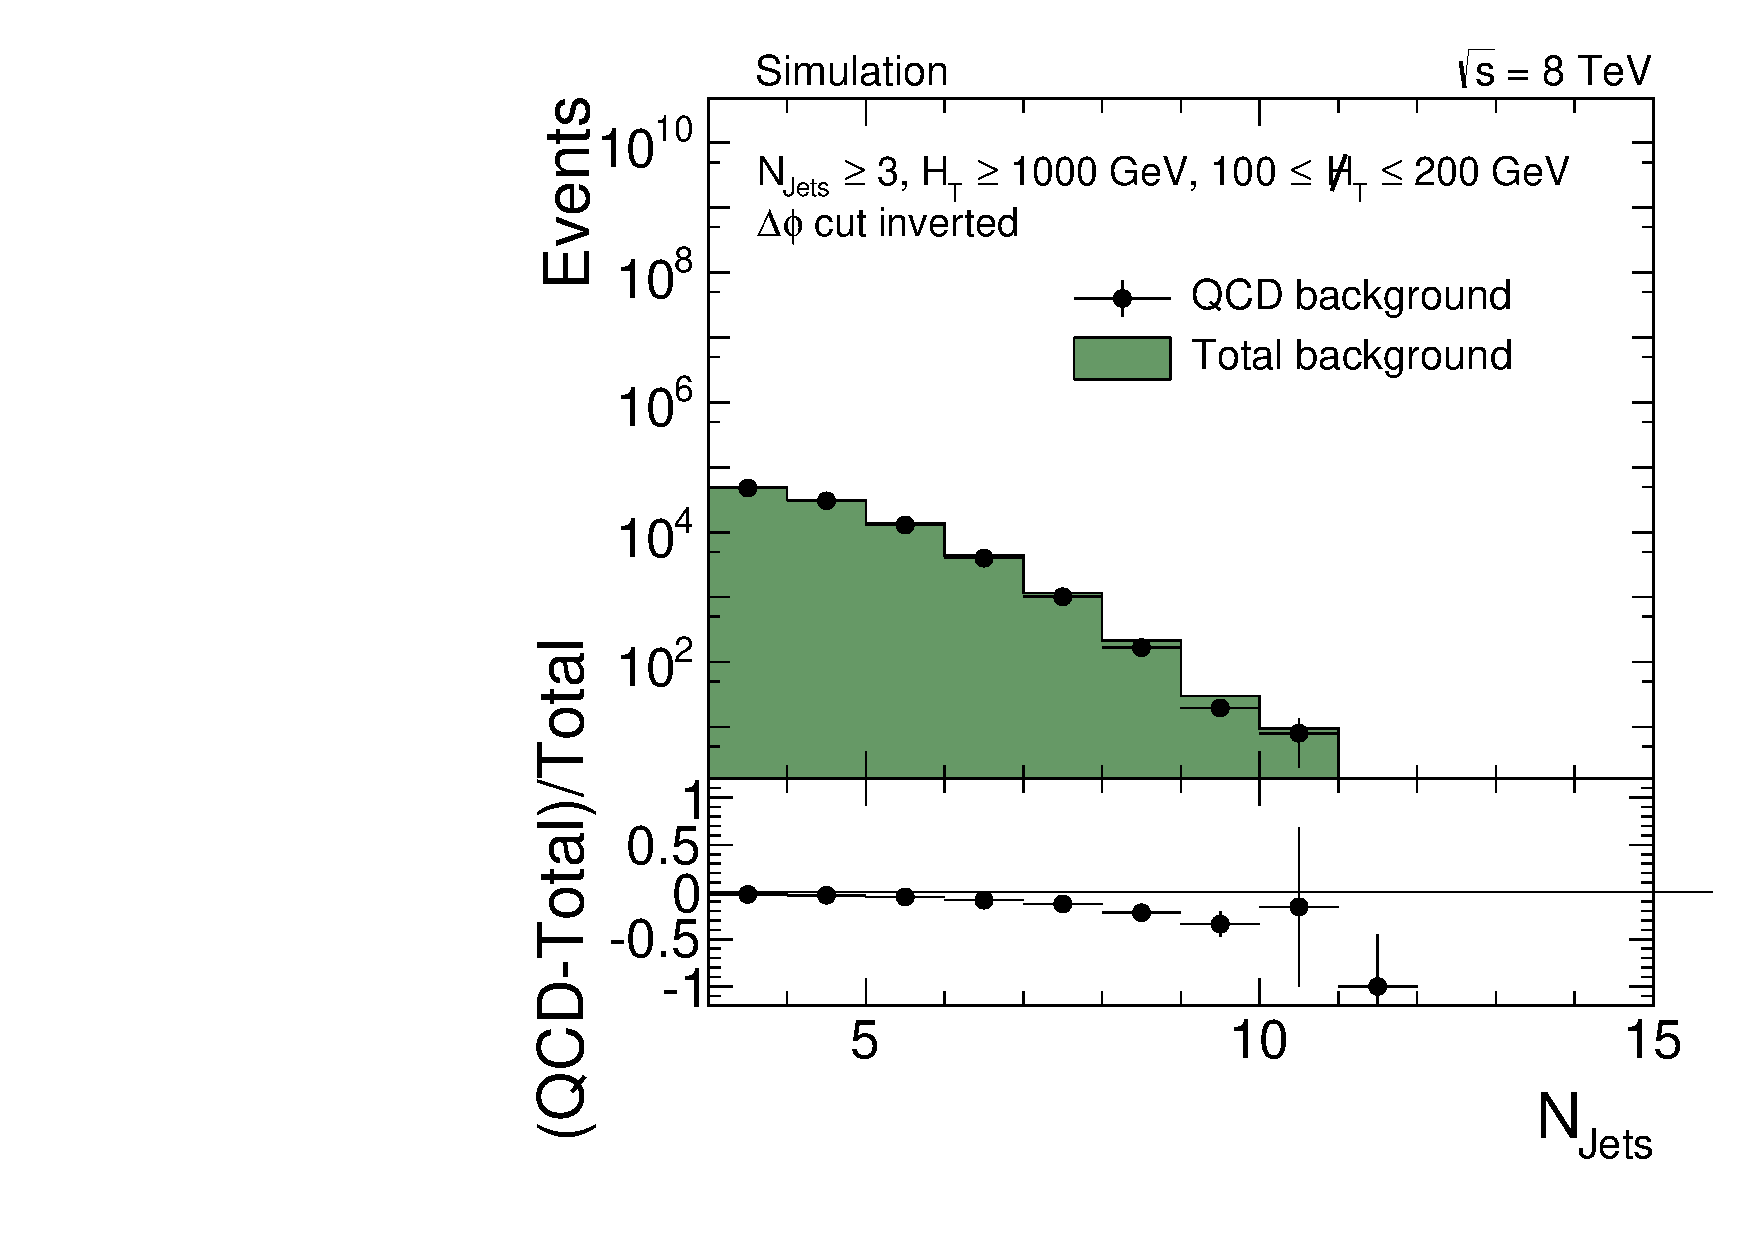
\includegraphics[width=0.49\textwidth]{figures/NJetsRA2_MC.pdf}
  \end{tabular}
  \caption{Prediction of QCD background on data compared to the expectation from data for a QCD enriched control region with \HT$>~1000~\rm{GeV}$, inverted $\Delta \phi$ cut, $\NJets \geq 3$ and $100 \leq \MHT \leq 200$\gev (\textit{upper row}) and selected QCD events in simulation compared to the total number of selected background events in simulation in the chosen control region (\textit{lower row}).}
  \label{fig:qcd_rs_dataclosure}
\end{figure}

\subsection{Systematic Uncertainties}
\label{subsec:RA2_syst_unc}
\subsubsection*{Core of response functions} The uncertainties on the factors of the Gaussian core resolution accounting for the differences in data and Monte Carlo denoted in Tab.~\ref{tab:jer_RPlusS_core} are propagated to the prediction. This is done by shifting the scaling factors by $\pm 1\sigma$ up and down. 
\subsubsection*{Tail of response functions} The uncertainties on the scaling factors of the non-Gaussian tails listed in Tab.~\ref{tab:jer_RPlusS_tails} are also propagated to the prediction by varying them within $\pm 1\sigma$ up and down. 
\subsubsection*{Bias uncertainty} The systematic uncertainty due to a potential non-closure and remaining biases of the R+S method is evaluated as described in Sec.~\ref{subsec:validation_mc}. This uncertainty also covers uncertainties on the rebalance correction factor and the jet-\pt cut value chosen for the jets considered in the rebalancing, such that no additional uncertainties are considered for those. The bias uncertainty is evaluated for each jet multiplicity bin separated into a low $ 500 \leq \HT \leq 1000$\gev and a high $\HT > 1000$\gev region.
\subsubsection*{Pileup} 
In general, the R+S method is taking care of influences from pileup by applying L1 jet energy corrections, making use of charged-hadron subtraction and neglecting soft jets in the rebalancing procedure. Furthermore, pileup, which is an issue especially for soft jets, does in general not contribute significantly to the high \MHT search bins, as these are mainly populated due to heavily mismeasured hard jets. \\
The residual pileup influence is evaluated in a low \MHT control region with \MHT $> 100 \rm{~GeV}$, since residual pileup effects are expected to contribute mostly in such low \MHT regions. Pileup contributions to the high \MHT signal regions might be even less, so that this approach provides a conservative estimate of the pileup uncertainty. Furthermore, the usage of a low \MHT control region ensures that statistical limitations are reduced.\\
The general approach is to estimate the pileup-dependent fraction of the nominal QCD prediction by studying the difference in the behaviour of the prediction in data and simulation (taken from \madgraph) for different pileup conditions. In order to do this, the sample is divided into three different bins of primary vertices $N_\mathrm{Vtx} = [0, 10]$, $N_\mathrm{Vtx} = [11, 20]$ and $N_\mathrm{Vtx} > 20$. Then, the QCD prediction is calculated for each vertex bin when applying baseline selection criteria with the relaxed \MHT requirement mentioned above. In order to compensate for the different number of seed events contributing to each $N_\mathrm{Vtx}$ interval, the prediction in each $N_\mathrm{Vtx}$ bin is normalized to the respective number of seed events contributing to that particular vertex bin. Furthermore, it is assumed that pileup effects are negligible in the lowest primary vertex bin. Hence, the predictions corrected for the number of seed events in data and simulation are normalized to each other, such that they have the same yield in the first primary vertex bin, in order to study the difference between data and MC prediction in the two higher primary vertex intervals. The distribution obtained with this procedure is illustrated for jet multiplicity 3--5 in Fig.~\ref{fig:qcd_rs_pileup}. 
\begin{figure}[!t]
  \centering
  \begin{tabular}{cc}
                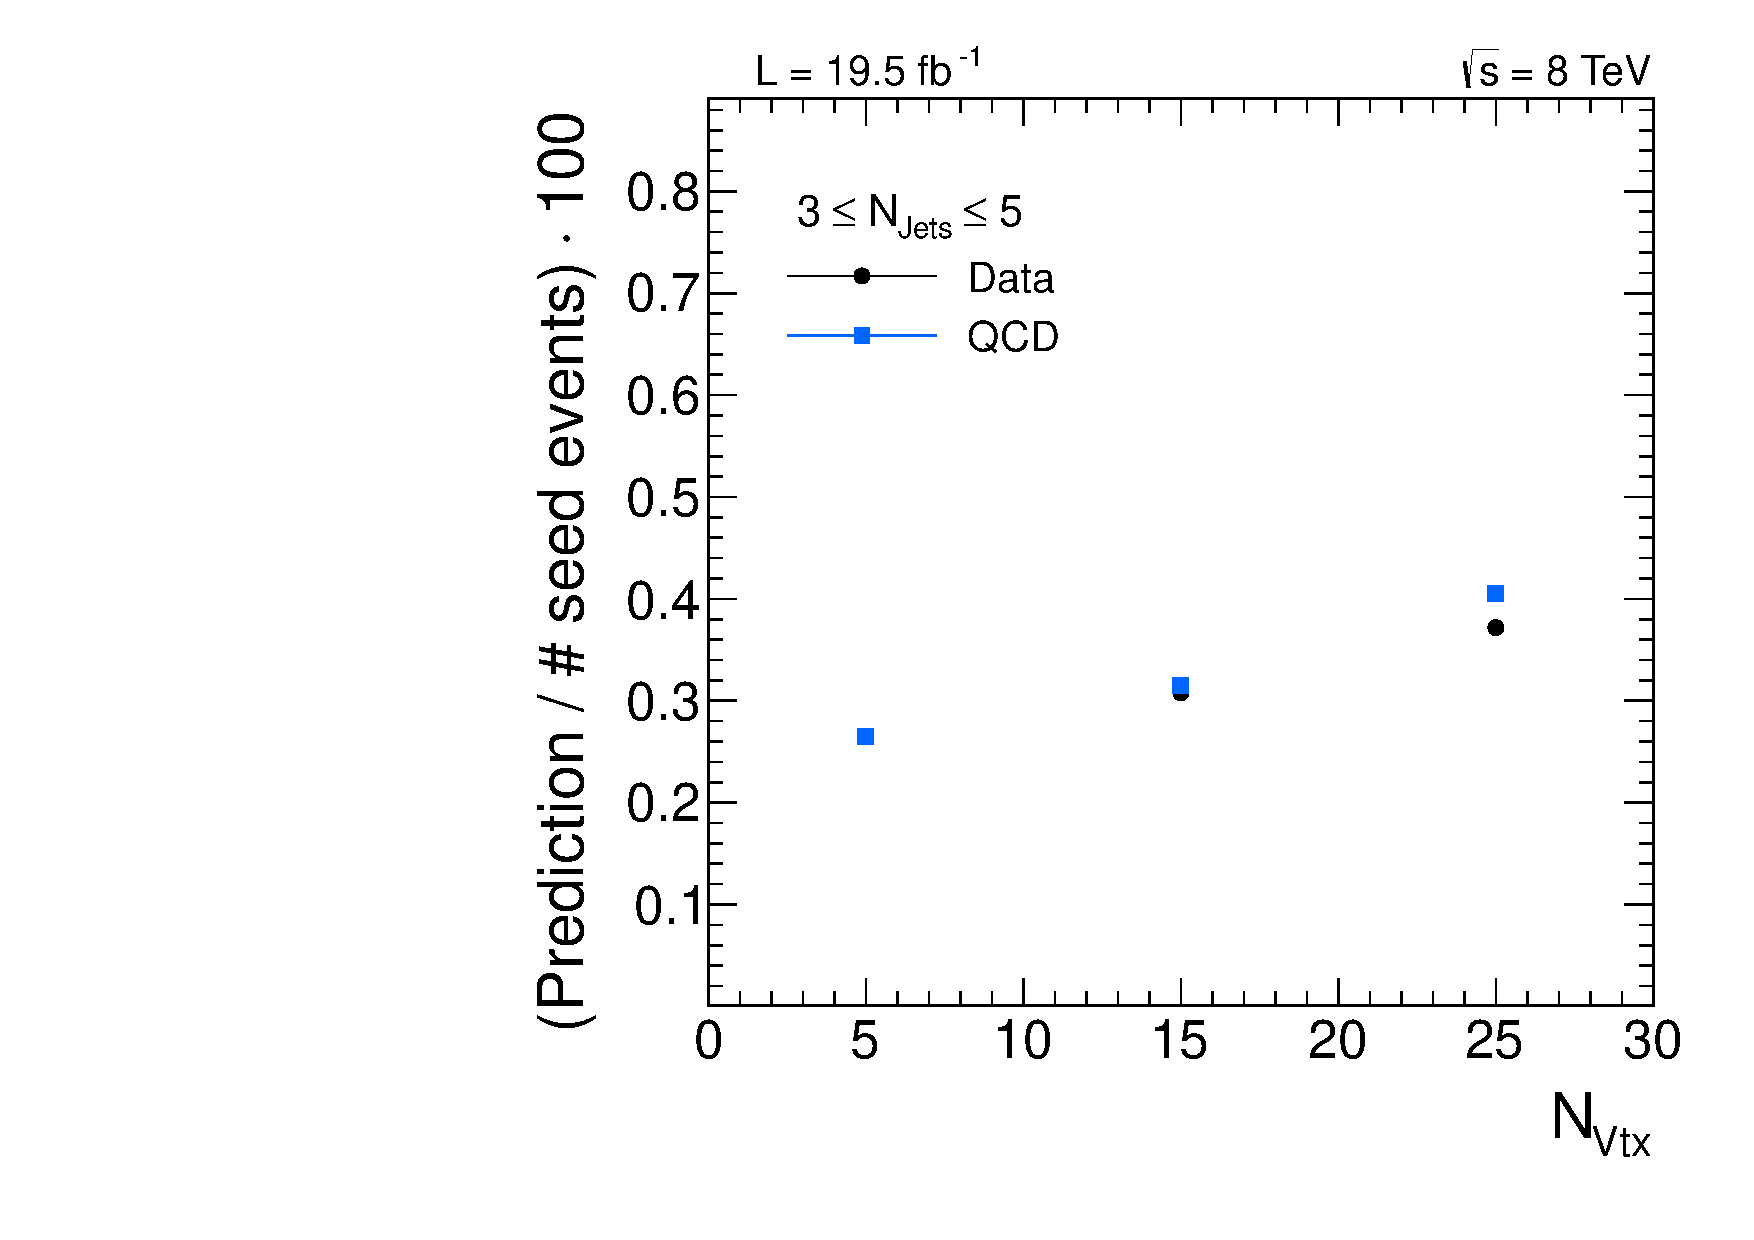
\includegraphics[width=0.49\textwidth]{figures/PUUncertainty_NJet3_5.pdf}% &
  %              \includegraphics[width=0.49\textwidth]{figures/PUUncertainty_NJet6_7.pdf} \\
  %              \multicolumn{2}{c}{\includegraphics[width=0.49\textwidth]{figures/PUUncertainty_NJet8.pdf}}
  \end{tabular}
  \caption{Prediction of QCD background in data and Monte Carlo as a function of primary vertices ($N_\mathrm{Vtx}$) normalized to the number of contributing seed events used for the determination of the pileup uncertainty as described in the text.}
  \label{fig:qcd_rs_pileup}
\end{figure}
In order to relate the observed difference between the data and MC prediction for different pileup conditions to the nominal QCD prediction in data, the absolute difference between data and Monte Carlo prediction for the second and the third vertex bin is taken, multiplied each with the seed events in data for that vertex bin and summed up.  %The input distributions for this calculation are illustrated in Fig.~\ref{fig:qcd_rs_pileup}. 
Finally, the ratio of this pileup dependent fraction of the prediction to the nominal QCD prediction is considered as pileup uncertainty. Due to statistical limitations it is not evaluated for the various \HT regions, but for the three jet multiplicity selections only. 

\subsection{QCD Background Prediction}
\label{subsec:RA2_qcd_pred}
The final prediction for QCD background contributions derived with the R+S method from a multijet control sample in data is summarized in Tab.~\ref{tab:QCDPred} for jet multiplicity bins 3--5, 6--7 and $\ge 8$. The quoted total systematic uncertainty is obtained by adding the single contributions in quadrature. \\
Some search bins show very large statistical uncertainties of $\geq 100 \%$. This then also affects the evaluation of systematic effects, \eg the core and tail scaling uncertainties. However, since this happens only in bins in which QCD background is almost negligible, it does not impact the final result of the analysis significantly. For the affected systematic variations, the largest observed variation is considered as systematic uncertainty, as a conservative estimate. Affected search bins are mainly the high \MHT and the highest jet multiplicity search bins. \\
However, search regions with non-negligible contributions from QCD background, like high \HT ($\ge 1000$\gev) and low \MHT bins, show in general quite moderate total uncertainties. Typical values lie around 50\% which is a remarkable precision for a prediction of a background that is so difficult to model, as discussed in the beginning of this section. The main contributions to the systematic uncertainty arise from the propagated uncertainties of the core and tail scaling factors. The resulting variations in the prediction from the variation of the core scaling factors are typically between 10--30 $\%$ in the search bins with non-negligible QCD contributions while it is between 20--35 $\%$ from the tail scaling factors. This emphasizes the importance to precisely measure the resolution data-to-simulation scale factors, as described in Chap.~\ref{chap:Resolution} for the scaling factors of the response core. 
\begin{table}[!hp]
  \centering
  \caption{Predicted event yields for the QCD background in the search regions defined by \HT, \MHT and \NJets shown together with statistical and systematic uncertainties. The uncertainties of the different systematic uncertainty sources are added in quadrature to obtain the total systematic uncertainties.}
  \label{tab:QCDPred}
 \resizebox{\textwidth}{!}{%
%  \makebox[\linewidth]{
    % \begin{tabular*}{\textwidth}{lll@{\extracolsep{\fill}}|r|r|r|r|r|r}
   % \begin{tabular}{lll|r|l|c|c|c|c|c}
    \begin{tabular}{lll|rc|cccc|c}
      \multicolumn{10}{c}{} \\
    

  %    \NJets{} & \HT{} [GeV] &\MHT{} [GeV]
      \NJets{} & \HT{} [GeV]& \MHT{} [GeV] & Pred. & stat. unc. & Core [\%] & Tail [\%] & Bias [\%] & PU [\%] & syst. unc. \\
      \midrule
      3--5     & 500--800  & 200--300 & 307.4 & $\pm$  18.5  & $^{+13.0}_{-12.2}$ & $^{36.0}_{-34.4} $ & $\pm$ 60.4 & $\pm$ 2.9 & $^{+220}_{-217}$  \\
      3--5     & 500--800  & 300--450 & 34.5  & $\pm$  5.8   & $^{+7.3}_{-10.5}$ & $^{22.9}_{-31.6} $  & $\pm$ 60.4 & $\pm$ 2.9 & $^{+22.4}_{-23.8}$ \\
      3--5     & 500--800  & 450--600 & 1.3   & $\pm$  1.2   & $^{+24.2}_{-16.7}$ & $^{+37.9}_{-26.5}$ &  $\pm$ 60.4 & $\pm$ 2.9 & $^{+1.0}_{-0.9}$  \\
      3--5     & 500--800  & $>600$  & 0.1   & $\pm$  0.3   & $^{+55.6}_{-55.6}$ & $^{+55.6}_{-55.6}$ & $\pm$  60.4 & $\pm$ 2.9 & $^{+0.09}_{-0.09}$\\ 
      \midrule
      3--5    & 800--1000  & 200--300 & 91.7  & $\pm$  10.2  & $^{+14.7}_{-13.8}$  & $^{+33.2}_{-33.5}$ & $\pm$  60.4 & $\pm$ 2.9 & $^{+64.7}_{-64.7}$\\
      3--5    & 800--1000  & 300--450 & 9.9   & $\pm$  3.2   & $^{+5.2}_{-5.1}$ & $^{+29.8}_{-27.1}$  & $\pm$  60.4  & $\pm$ 2.9 & $^{+6.7}_{-6.6}$ \\
      3--5    & 800--1000  & 450--600 & 0.8   & $\pm$  0.9  & $^{+65.5}_{-65.5}$ &  $^{+65.5}_{-65.5}$ & $\pm$  60.4 & $\pm$ 2.9 & $^{+0.9}_{-0.8}$  \\
      3--5    & 800--1000  & $>600$  & 0.1   & $\pm$  0.4  & $^{+75.0}_{-41.7}$ &  $^{+8.3}_{-41.7}$  & $\pm$  60.4 & $\pm$ 2.9 & $^{+0.1}_{-0.1}$  \\
      \midrule
      3--5   & 1000--1250  & 200--300 & 59.0  & $\pm$  7.2  & $^{+19.0}_{-14.6}$ & $^{+34.7}_{-31.7}$ & $\pm$  14.5   & $\pm$ 2.9 & $^{+24.9}_{-22.4}$\\
      3--5   & 1000--1250  & 300--450 & 5.1   & $\pm$  2.2  & $^{+12.2}_{-8.8}$ & $^{+32.0}_{-16.9}$ & $\pm$  14.5   & $\pm$ 2.9 & $^{+1.9}_{-1.2}$ \\
      3--5   & 1000--1250  & 450--600 & 0.5   & $\pm$  0.7  & $^{+35.3}_{-3.9}$ & $^{+23.5}_{-5.9}$ &  $\pm$  14.5   & $\pm$ 2.9 & $^{+0.2}_{-0.1}$ \\
      3--5   & 1000--1250  & $>600$  & 0.1   & $\pm$  0.3  & $^{+41.7}_{-41.7}$ & $^{+41.7}_{-41.7}$ & $\pm$ 14.5   &  $\pm$ 2.9 & $^{+0.1}_{-0.1}$ \\
      \midrule
      3--5   & 1250--1500  & 200--300 & 31.2  & $\pm$  5.3  & $^{+18.3}_{-19.1}$ & $^{+30.3}_{-29.7}$ & $\pm$  14.5  & $\pm$ 2.9 & $^{+12.0}_{-11.9}$\\
      3--5   & 1250--1500  & 300--450 & 2.3   & $\pm$  1.3  & $^{+16.3}_{-5.3}$ & $^{+38.3}_{-30.4}$ & $\pm$  14.5  & $\pm$ 2.9 & $^{+1.0}_{-0.8}$ \\
      3--5   & 1250--1500  & $>450$  & 0.2   & $\pm$  0.5  & $^{+0.0}_{-8.3}$ & $^{+54.2}_{-8.3}$  & $\pm$   14.5 & $\pm$ 2.9 & $^{+0.1}_{-0.1}$  \\
      \midrule
      3--5   & $>$1500    & 200--300 & 35.1  & $\pm$  6.1  & $^{+19.6}_{-20.0}$ & $^{+23.3}_{-29.4}$ & $\pm$   14.5 & $\pm$ 2.9 & $^{+11.9}_{-13.5}$ \\
      3--5   & $>$1500    & $>300$  & 2.4   & $\pm$  1.4  & $^{+39.9}_{-39.9}$ & $^{+39.9}_{-39.9}$ & $\pm$   14.5 & $\pm$ 2.9 & $^{+1.4}_{-1.4}$ \\
      \midrule 
      \midrule
      6--7   & 500--800   & 200--300  &  18.2 & $\pm$  3.9  & $^{+8.9}_{-12.5}$ & $^{+37.4}_{-33.5}$ & $\pm$  25.4  & $\pm$ 8.0 & $^{+8.5}_{-8.1}$  \\
      6--7   & 500--800   & 300--450  &  1.9  & $\pm$  1.4  & $^{+31.9}_{-31.9}$ & $^{+31.9}_{-31.9}$ & $\pm$  25.4 & $\pm$ 8.0 & $^{+1.0}_{-1.0}$  \\
      6--7   & 500--800   & $>450$   &  0.01 & $\pm$  0.1  & $^{+400.0}_{-100.0}$ & $^{+400.0}_{-100.0}$ & $\pm$  25.4 & $\pm$ 8.0 & $^{+0.1}_{-0.01}$\\
      \midrule
      6--7   & 800--1000  & 200--300  &  13.13& $\pm$  3.4  & $^{+15.0}_{-8.2}$ & $^{+33.7}_{-30.0}$ & $\pm$  25.4  & $\pm$ 8.0 & $^{+6.0}_{-5.3}$  \\
      6--7   & 800--1000  & 300--450  &  2.0  & $\pm$  1.1  & $^{+5.1}_{-20.0}$ & $^{+30.8}_{-28.2}$ & $\pm$  25.4  & $\pm$ 8.0 & $^{+0.8}_{-0.9}$  \\
      6--7   & 800--1000  & $>450$   &  0.2  & $\pm$  0.4  & $^{+46.7}_{-46.7}$ & $^{+46.7}_{-46.7}$ & $\pm$  25.4 & $\pm$ 8.0 & $^{+0.1}_{-0.1}$  \\ 
      \midrule
      6--7   & 1000--1250 & 200--300  &  11.9 & $\pm$  3.8  & $^{+5.9}_{-12.7}$ & $^{+33.5}_{-35.8}$  & $\pm$  10.9 & $\pm$ 8.0 & $^{+4.4}_{-4.8}$ \\
      6--7   & 1000--1250 & 300--450  &  1.5  & $\pm$  1.3  & $^{+31.8}_{-31.8}$ & $^{+31.8}_{-31.8}$  & $\pm$  10.9 &  $\pm$ 8.0 & $^{+0.7}_{-0.7}$ \\
      6--7   & 1000--1250 & $>450$   &  0.1  & $\pm$  0.3  & $^{+100.0}_{-100.0}$ & $^{+100.0}_{-100.0}$ & $\pm$  10.9 & $\pm$ 8.0 & $^{+0.2}_{-0.1}$ \\
      \midrule
      6--7   & 1250--1500 & 200--300  &  6.8  & $\pm$  3.0  & $^{+12.0}_{-11.9}$ & $^{+32.6}_{-32.4}$ & $\pm$   10.9   & $\pm$ 8.0 & $^{+2.5}_{-2.5}$ \\
      6--7   & 1250--1500 & 300--450  &  0.9  & $\pm$  1.0  & $^{+54.4}_{-54.4}$ & $^{+54.4}_{-54.4}$ & $\pm$   10.9   & $\pm$ 8.0 & $^{+0.7}_{-0.7}$ \\
      6--7   & 1250--1500 & $>450$   &  0.09 & $\pm$  0.3  & $^{+44.4}_{-44.4}$ & $^{+44.4}_{-44.4}$ & $\pm$   10.9  & $\pm$ 8.0 & $^{+0.06}_{-0.06}$\\
      \midrule
      6--7   & $>$1500   & 200--300  &  8.0  & $\pm$  2.8  & $^{+20.9}_{-15.4}$ & $^{+31.5}_{-25.8}$ & $\pm$   10.9  & $\pm$ 8.0 & $^{+3.1}_{-2.6}$\\
      6--7   & $>$1500   & $>300$   &  0.8  & $\pm$  0.9  & $^{+47.0}_{-47.0}$ & $^{+47.0}_{-47.0}$ & $\pm$   10.9  & $\pm$ 8.0 & $^{+0.6}_{-0.6}$ \\
      \midrule 
      \midrule 
      $\geq$8 & 500--800 & $>200$   &  0.14 & $\pm$  0.38 & $^{+71.4}_{-71.4}$ & $^{+71.4}_{-71.4}$ & $\pm$ 86.0  & $\pm$ 33.4 & $^{+0.19}_{-0.14}$ \\
      $\geq$8 & 800--1000 & $>200$  &  0.54 & $\pm$  0.69 & $^{+33.3}_{-33.3}$ & $^{+33.3}_{-33.3}$ & $\pm$ 86.0  & $\pm$ 33.4 & $^{+0.56}_{-0.54}$ \\
      $\geq$8 & 1000--1250 & $>200$ &  0.73 & $\pm$  0.78 & $^{+19.2}_{-1.4}$ & $^{+56.2}_{-27.4}$  & $\pm$ 86.0 & $\pm$ 33.4 & $^{+0.59}_{-0.44}$ \\
      $\geq$8 & 1250--1500 & $>200$ &  0.54 & $\pm$  0.75 & $^{+55.6}_{-55.6}$ & $^{+55.6}_{-55.6}$ & $\pm$ 86.0 & $\pm$ 33.4 & $^{+0.52}_{-0.52}$ \\
      $\geq$8 & $>$1500   & $>200$ &  0.89 & $\pm$  0.94 & $^{+65.2}_{-65.2}$ & $^{+65.2}_{-65.2}$ & $\pm$ 86.0 & $\pm$ 33.4 & $^{+0.95}_{-0.89}$ \\
      \bottomrule
    \end{tabular}}
  % \end{lrbox}
  % \scalebox{0.95}{\usebox{\closureBox}}
  % }
  % \end{center}
\end{table}

\section{Results and Interpretation}
\label{sec:RA2_results}
The selected number of events in 19.5\fbinv of data together with the predicted event yields for the various SM background contributions estimated as discussed in Sec.~\ref{sec:RA2_Non-QCD} and Sec.~\ref{subsec:RA2_QCD}, are listed in Tab.~\ref{tab:FinalEventYields} for all 36 exclusive search regions. The displayed uncertainties for the background predictions are the total uncertainties. Furthermore, the obtained yields in data and the predicted background are visualized in Fig.~\ref{fig:ra2_summary}. The ratio in the bottom shows the difference between observed data events and predicted background normalized to the background prediction. In general, the data are consistent with the SM expectation. The largest deviation occurs in the search region for $6 \leq \NJets \leq 7$, $500 < \HT < 800$\gev and $\MHT \ge 450$\gev with a local p-value of 0.05. However, this is insignificant when including the probability to observe a statistical fluctuation as large or larger in any of the search regions corresponding to a global p-value of 0.78. 
\begin{table}[!hp]
  \centering
  \caption{Predicted event yields for the different background components in the search regions defined by \HT, \MHT and \NJets. The uncertainties of the different background sources are added in quadrature to obtain the total uncertainties. Taken from~\cite{Chatrchyan:2014lfa}.
  }
  \label{tab:FinalEventYields}
 \resizebox{\textwidth}{!}{%
%  \makebox[\linewidth]{
    % \begin{tabular*}{\textwidth}{lll@{\extracolsep{\fill}}|r|r|r|r|r|r}
    \begin{tabular}{lll|r|r|r|r|r|r}
      \multicolumn{9}{c}{} \\
      \multicolumn{3}{c|}{Selection}
      & \multicolumn{1}{c|}{$Z \rightarrow \nu\bar{\nu}$} 
      & \multicolumn{1}{c|}{$\ttbar/W$}
      & \multicolumn{1}{c|}{$\ttbar/W$} 
      & \multicolumn{1}{c|}{QCD}
      & \multicolumn{1}{c|}{Total }
      & \multicolumn{1}{c}{Data}          \\

      \NJets{} & \HT{} [GeV] &\MHT{} [GeV]
      & \multicolumn{1}{c|}{} 
      & \multicolumn{1}{c|}{$\to \e,\mu+$X}
      & \multicolumn{1}{c|}{$\to \tau_{\mbox{\tiny h}}+$X}  
      & \multicolumn{1}{c|}{}
      & \multicolumn{1}{c|}{background}  
      & \multicolumn{1}{c}{}  \\ 
      % \hspace*{-2ex}
      \hline
      3--5     & 500--800    & 200--300  & 1821   $\pm$  387         & 2211   $\pm$  448        &1749   $\pm$  210        & 307  $\pm$  219         & 6088   $\pm$  665      &  6159  \\
      3--5     & 500--800    & 300--450  &  994   $\pm$  218         &  660   $\pm$  133        & 590   $\pm$   69        & 35   $\pm$   24         & 2278   $\pm$  266      &  2305  \\
      3--5     & 500--800    & 450--600  &  273   $\pm$   63         &   77   $\pm$   17        &  66.3 $\pm$   9.5       &  1.3 $^{+1.5}_{-1.3}$       & 418    $\pm$   66      &   454  \\
      3--5     & 500--800    & $>600$   &   42   $\pm$   10         &   9.5 $\pm$    4.0       &   5.7 $\pm$   1.3       &  0.1 $^{+0.3}_{-0.1}$       & 57.4   $\pm$   11.2    &    62  \\ \hline
      3--5     & 800--1000   & 200--300  &  216   $\pm$   46         &  278   $\pm$   62        & 192   $\pm$   33        & 92   $\pm$   66         & 777    $\pm$  107      &   808  \\
      3--5     & 800--1000   & 300--450  &  124   $\pm$   26         &  113   $\pm$   27        &  84   $\pm$   12        &  9.9 $\pm$    7.4       & 330    $\pm$   40      &   305  \\
      3--5     & 800--1000   & 450--600  &   47   $\pm$   11         &   36.1 $\pm$    9.9      &  24.1 $\pm$    3.6      &  0.8 $^{+1.3}_{-0.8}$       & 108    $\pm$   15      &   124  \\
      3--5     & 800--1000   & $>600$   &   35.3 $\pm$    8.8       &    9.0 $\pm$    3.7      &  10.3 $\pm$    2.0      &  0.1 $^{+0.4}_{-0.1}$       & 54.8   $\pm$   9.7     &    52  \\ \hline
      3--5     & 1000--1250  & 200--300  &   76   $\pm$   17         &  104   $\pm$   26        &  66.5 $\pm$    9.9      & 59   $\pm$   25         & 305    $\pm$   41      &   335  \\
      3--5     & 1000--1250  & 300--450  &   39.3 $\pm$    8.9       &   52   $\pm$   14        &  41   $\pm$   11        &  5.1 $\pm$    2.7       & 137    $\pm$   20      &   129  \\
      3--5     & 1000--1250  & 450--600  &   18.1 $\pm$    4.7       &    6.9 $\pm$    3.2      &   6.8 $\pm$    2.0      &  0.5 $^{+0.7}_{-0.5}$       & 32.3   $\pm$    6.1    &    34  \\
      3--5     & 1000--1250  & $>600$   &   17.8 $\pm$    4.8       &    2.4 $\pm$    1.8      &   2.5 $\pm$    0.8      &  0.1 $^{+0.3}_{-0.1}$       & 22.8   $\pm$    5.2    &    32  \\ \hline
      3--5     & 1250--1500  & 200--300  &   25.3 $\pm$    6.0       &   31.0 $\pm$    9.5      &  21.3 $\pm$    4.1      & 31   $\pm$   13         & 109    $\pm$   18      &    98  \\
      3--5     & 1250--1500  & 300--450  &   16.7 $\pm$    4.3       &   10.1 $\pm$    4.4      &  13.7 $\pm$    7.1      &  2.3 $\pm$    1.6       & 42.8   $\pm$    9.5    &    38  \\
      3--5     & 1250--1500  & $>450$   &   12.3 $\pm$    3.5       &    2.3 $\pm$    1.7      &   2.7 $\pm$    1.2      &  0.2 $^{+0.5}_{-0.2}$       & 17.6   $\pm$    4.1    &    23  \\ \hline
      3--5     & $>$1500    & 200--300  &   10.5 $\pm$    2.9       &   16.7 $\pm$    6.2      &  23.5 $\pm$    5.6      & 35   $\pm$   14         & 86     $\pm$   17      &    94  \\
      3--5     & $>$1500    & $>300$   &   10.9 $\pm$    3.1       &    9.7 $\pm$    4.3      &   6.6 $\pm$    1.4      &  2.4 $\pm$    2.0       & 29.7   $\pm$    5.8    &    39  \\ \hline \hline
      6--7     & 500--800    & 200--300  &   22.7 $\pm$    6.4       &  133   $\pm$   59        & 117   $\pm$   25        & 18.2 $\pm$    9.2       & 290    $\pm$   65      &   266  \\
      6--7     & 500--800    & 300--450  &    9.9 $\pm$    3.2       &   22   $\pm$   11        &  18.0 $\pm$    5.1      &  1.9 $\pm$    1.7       & 52     $\pm$   12      &    62  \\
      6--7     & 500--800    & $>450$   &    0.7 $\pm$    0.6       &    0.0 $^{+3.2}_{-0.0}$      &   0.1 $^{+0.5}_{-0.1}$      &  0.0 $^{+0.1}_{-0.0}$       & 0.8    $^{+3.3}_{-0.6}$    &     9  \\ \hline
      6--7     & 800--1000   & 200--300  &    9.1 $\pm$    3.0       &   56   $\pm$   25        &  46   $\pm$   11        & 13.1 $\pm$    6.6       & 124    $\pm$   29      &   111  \\
      6--7     & 800--1000   & 300--450  &    4.2 $\pm$    1.7       &   10.4 $\pm$    5.5      &  12.0 $\pm$    3.6      &  1.9 $\pm$    1.4       & 28.6   $\pm$    6.9    &    35  \\
      6--7     & 800--1000   & $>450$   &    1.8 $\pm$    1.0       &    2.9 $\pm$    2.5      &   1.2 $\pm$    0.8      &  0.1 $^{+0.4}_{-0.1}$       & 6.0    $\pm$    2.8    &     4  \\ \hline
      6--7     & 1000--1250  & 200--300  &    4.4 $\pm$    1.7       &   24   $\pm$   12        &  29.5 $\pm$    7.8      & 11.9 $\pm$    6.0       &  70    $\pm$   16      &    67  \\
      6--7     & 1000--1250  & 300--450  &    3.5 $\pm$    1.5       &    8.0 $\pm$    4.7      &   8.6 $\pm$    2.7      &  1.5 $\pm$    1.5       & 21.6   $\pm$    5.8    &    20  \\
      6--7     & 1000--1250  & $>450$   &    1.4 $\pm$    0.8       &    0.0 $^{+3.6}_{-0.0}$      &   0.6 $^{+0.8}_{-0.6}$      &  0.1 $^{+0.4}_{-0.1}$       & 2.2    $^{+3.8}_{-1.1}$    &     4  \\ \hline
      6--7     & 1250--1500  & 200--300  &    3.3 $\pm$    1.4       &   11.5 $\pm$    6.5      &   6.4 $\pm$    2.7      &  6.8 $\pm$    3.9       & 28.0   $\pm$    8.2    &    24  \\
      6--7     & 1250--1500  & 300--450  &    1.4 $\pm$    0.8       &    3.5 $\pm$    2.6      &   3.5 $\pm$    1.9      &  0.9 $^{+1.3}_{-0.9}$       & 9.4    $\pm$    3.6    &     5  \\
      6--7     & 1250--1500  & $>450$   &    0.4 $\pm$    0.4       &    0.0 $^{+2.5}_{-0.0}$      &   0.1 $^{+0.5}_{-0.1}$      &  0.1 $^{+0.3}_{-0.1}$       & 0.5    $^{+2.6}_{-0.4}$    &     2  \\ \hline
      6--7     & $>$1500    & 200--300  &    1.3 $\pm$    0.8       &   10.0 $\pm$    6.9      &   2.0 $\pm$    1.2      &  7.8 $\pm$    4.0       & 21.1   $\pm$    8.1    &    18  \\
      6--7     & $>$1500    & $>300$   &    1.1 $\pm$    0.7       &    3.2 $\pm$    2.8      &   2.8 $\pm$    1.9      &  0.8 $^{+1.1}_{-0.8}$       & 7.9    $\pm$    3.6    &     3  \\ \hline \hline 
      $\geq$8 & 500--800    & $>200$   &    0.0 $^{+0.8}_{-0.0}$       &    1.9 $\pm$    1.5      &   2.8 $\pm$    1.4      &  0.1 $^{+0.4}_{-0.1}$       & 4.8    $^{+2.3}_{-2.1}$    &     8  \\
      $\geq$8 & 800--1000   & $>200$   &    0.6 $\pm$    0.6       &    4.8 $\pm$    2.9      &   2.3 $\pm$    1.2      &  0.5 $^{+0.9}_{-0.5}$       & 8.3    $^{+3.4}_{-3.3}$    &     9  \\
      $\geq$8 & 1000--1250  & $>200$   &    0.6 $\pm$    0.5       &    1.4 $^{+1.5}_{-1.4}$      &   2.9 $\pm$    1.3      &  0.7 $^{+1.0}_{-0.7}$       & 5.6    $^{+2.3}_{-2.1}$    &     8  \\
      $\geq$8 & 1250--1500  & $>200$   &    0.0 $^{+0.9}_{-0.0}$       &    5.1 $\pm$    3.5      &   1.4 $\pm$    0.9      &  0.5 $^{+0.9}_{-0.5}$       & 7.1    $^{+3.8}_{-3.6}$    &     5  \\
      $\geq$8 & $>$1500    & $>200$   &    0.0 $^{+0.7}_{-0.0}$       &    0.0 $^{+4.2}_{-0.0}$      &   2.4 $\pm$    1.4      &  0.9 $^{+1.3}_{-0.9}$       & 3.3    $^{+4.7}_{-1.7}$    &     2  \\ \hline \hline


    \end{tabular}}
  % \end{lrbox}
  % \scalebox{0.95}{\usebox{\closureBox}}
  % }
  % \end{center}
\end{table}
\begin{figure}[!hp]
  \centering
  \begin{tabular}{c}
    \includegraphics[width=0.99\textwidth]{figures/RA2_summary.pdf}
  \end{tabular}
  \caption{Summary of the observed number of events in each of the 36 search regions in comparison to the corresponding background prediction. The hatched region shows the total uncertainty of the background prediction. Taken from~\cite{Chatrchyan:2014lfa}.}
  \label{fig:ra2_summary}
\end{figure}
\\
\\
Furthermore, the results are interpreted in several simplified supersymmetric models of pair production of light-flavour squarks or gluinos. The LSP is denoted as $\tilde{\chi}_1^0$. Several different decay modes are studied in the parameter space of the LSP and the squark or gluino which are
\begin{description}
\item (a) $\tilde{q} \rightarrow q + \tilde{\chi}_1^0$
\end{description} 
in case of light-flavour squarks and
\begin{description}
\item (b) $\tilde{g} \rightarrow q\bar{q} + \tilde{\chi}_1^0$
\item (c) $\tilde{g} \rightarrow t\bar{t} + \tilde{\chi}_1^0$
\item (d) $\tilde{g} \rightarrow q\bar{q} + \tilde{\chi}_1^{\pm}/\tilde{\chi}_2^0 \;\; \mathrm{where} \;\; \tilde{\chi}_1^{\pm} \rightarrow W + \tilde{\chi}_1^0, \; \tilde{\chi}_2^0 \rightarrow Z + \tilde{\chi}_1^0 \;\; \mathrm{and} \;\; m_{\tilde{\chi}_1^{\pm}/\tilde{\chi}_2^0} = 0.5(m_{{\tilde{\chi}^0_1}} + m_{\tilde{g}})$ 
\end{description}  
for decays of the gluino. The branching ratios are assumed to be 100\% for the different decay modes, except for case (d) where the decay via $\tilde{\chi}_1^{+}$, $\tilde{\chi}_1^{-}$ and $\tilde{\chi}_2^0$ is considered with equal probabilities. \\
Exclusion limits are derived with the modified $\mathrm{CL_s}$~\cite{0954-3899-28-10-313, Thomas1999435, bib:Higgs:CLS} approach and denote the 95\% confidence level (CL) upper limit on the production cross section of the signal. The profile likelihood ratio is used as test statistics which is derived from the combined likelihood calculated for all 36 search regions considering the uncertainties of the acceptance, efficiencies and uncertainties for the signal as well as the background predictions. The uncertainties considered for the signal acceptance and efficiency in the limit setting procedure are: 
\begin{itemize} 
\item 2.6\% uncertainty on the integrated luminosity~\cite{CMS-PAS-LUM-13-001}
\item 2\% uncertainty for a possible trigger inefficiency (cf. Sec.~\ref{subsec:RA2_samples_trigger})
\item 3\% uncertainty due to a possible mismodelling of the event cleaning efficiency
\item 2--8\% and 1--2\% in the signal acceptance from the propagation of the respective uncertainties on the jet energy calibration and resolution 
\item 1--8\% in the signal acceptance from the systematic variation of PDFs~\cite{Botje:2011sn} 
\item an uncertainty considering the adjustment of the rate of initial-state radiation in simulation to match the measured rate in data~\cite{isrfsr} resulting for model parameter points with small differences between the LSP and the gluino or squark mass in an uncertainty of up to 22\% and typically less than a few percent for others  
\end{itemize}
\begin{figure}[!t]
  \centering
  \begin{tabular}{cc}
                \includegraphics[width=0.49\textwidth]{figures/RA2_Limit1.pdf} &
                \includegraphics[width=0.49\textwidth]{figures/RA2_Limit2.pdf} \\
                \includegraphics[width=0.49\textwidth]{figures/RA2_Limit3.pdf} &
                \includegraphics[width=0.49\textwidth]{figures/RA2_Limit4.pdf} \\
  \end{tabular}
\caption{The observed and expected 95\% CL upper limits on the (a) squark-squark and (b--d) gluino-gluino production cross sections in either the m(squark)-m(LSP) or the m(gluino)-m(LSP) plane obtained with the simplified models. For the squark-squark production the upper set of curves corresponds to the scenario when the first two generations of squarks are degenerate and light, while the lower set corresponds to only one light accessible squark~\cite{Chatrchyan:2014lfa}.} 
  \label{fig:ra2_limits}
\end{figure}
Finally, the resulting exclusion limits for the above described processes (a)--(d) are shown in Fig.~\ref{fig:ra2_limits}(a)--(d), respectively. The expected (\textit{dashed}) and observed (\textit{solid}) 95\% CL upper limits are shown in the gluino-LSP and squark-LSP mass plane for the signal production cross sections, respectively. The one-standard-deviation uncertainty for the theory prediction is obtained by varying the renormalization and factorization scale by a factor of two and incorporating CTEQ6.6~\cite{Nadolsky:2008zw} and MSTW2008~\cite{Martin:2009iq} as alternative PDF sets. By considering conservatively the observed limit minus the one sigma theory uncertainty, pair production of squarks of the first two generations is excluded below 780\gev for a LSP mass less than 200\gev. However, if only one light squark is accessible, the limit decreases to 400\gev for LSP masses below 80\gev. Similarly, the pair production of gluinos could be excluded for the three different decay modes (b)--(d) in case of a LSP mass less than 100\gev for gluino masses up to 1.16\tev, 1.13\tev and 1.21\tev, respectively. \\
In general, the analysis provides good sensitivity to signal points with large mass differences between squark/gluino and LSP mass, nearly independent of the LSP mass. This is due to the fact that for such mass scenarios the selection based on large values of \HT and \MHT is most efficient. For signal scenarios in which the mass difference between squark/gluino and LSP is small, softer jets and smaller values of \MHT are expected and consequently the analysis sensitivity drops resulting in the weaker cross section limits.

\subsection{Comparison to Other Measurements}
\label{subsec:RA2_comp}
The exclusion limits obtained with the analysis presented in this thesis exceed the exclusion limits derived from the 7\tev analysis (cf. Fig.~\ref{fig:SMS_7TeV}). Especially, the limit on the gluino mass is improved by around 200\gev for light LSPs. Furthermore, the extension of the analysis into the \NJets plane provides a good sensitivity towards the gluino-mediated production of third generation squarks and to decays involving $W$ and $Z$ bosons which could not be explored before. \\
Furthermore, studies using the $\sqrt{s} = 8$\tev data targeting the same simplified models, but based on different analysis techniques or final states, have been performed within CMS as well. A comparison of the analysis presented here (SUS-13-012) to other CMS analyses is illustrated in Fig.~\ref{fig:result_comp} for models (a)--(c) introduced in Sec.~\ref{sec:RA2_results}. 
\begin{figure}[!t]
  \centering
\makebox[\linewidth]{
  \begin{minipage}[c]{1.\linewidth}
    \begin{center}
      \includegraphics[width=0.49\textwidth]{figures/T1_ICHEP2014_All.png}% \hspace {1.5 pt} 
      \includegraphics[width=0.49\textwidth]{figures/T2_ICHEP2014.png}\\ 
      \includegraphics[width=0.49\textwidth]{figures/T1tttt_ICHEP2014_All.png}
    \end{center}
  \end{minipage}}

  \caption{Comparison of various exclusion limits derived by different CMS analyses for the process $\tilde{g} \rightarrow q\bar{q} + \tilde{\chi}_1^0$ (\textit{top left}), $\tilde{q} \rightarrow q + \tilde{\chi}_1^0$ (\textit{top right}) and $\tilde{g} \rightarrow t\bar{t} + \tilde{\chi}_1^0$ (\textit{bottom}). Taken from~\cite{bib:CMS:PhysicsResultsSUS}.}
  \label{fig:result_comp} 
\end{figure}
\\
This comparison exhibits that the expected sensitivity to the models $\tilde{g} \rightarrow q\bar{q} + \tilde{\chi}_1^0$ and $\tilde{q} \rightarrow q + \tilde{\chi}_1^0$ is similar for the different analyses. This is not unexpected as the compared analyses all make use of the all-hadronic final state. However, the analysis published in~\cite{CMS-PAS-SUS-13-019} performs better especially in case of squark production, as here also search regions based on dijet events are employed. \\
Concerning gluino-mediated stop production it is interesting to note that the analysis presented in this thesis is also similarly sensitive to this model as other all-hadronic searches (\cf SUS-12-028, SUS-12-024 or SUS-13-019). These other hadronic analyses typically employ b-tagging information while the analysis presented in this thesis followed a complementary approach by employing high jet multiplicity search regions. However, the best sensitivity to this respective model is achieved by an analysis which is based on a single lepton, multiple jets and b-tags (SUS-13-007). 
\\
Comparable analyses have also been performed by the ATLAS experiment~\cite{Aad:2014wea, Aad:2013wta, Aad:2014lra} and the obtained exclusion limits on sparticle masses lie in a very similar mass region.

\section{Status of supersymmetry after LHC Run I}
\label{sec:susy_status}
\begin{figure}[!t]
  \centering
  \begin{tabular}{cc}
                \includegraphics[width=0.49\textwidth]{figures/pMSSM_gluino.pdf} &
                \includegraphics[width=0.49\textwidth]{figures/pMSSM_squark.pdf} 
  \end{tabular}
\caption{Marginalized distributions of gluino masses (\textit{left}) and $\tilde{u}_L,\tilde{c}_L$ masses (\textit{right}). Filled histograms show prior distributions while line histograms illustrate posterior distributions based on the results of the analysis presented in this chapter and~\cite{Chatrchyan:2012lia}. Solid curves denote the nominal curves while dashed lines represent systematic variations. Taken from~\cite{CMS-PAS-SUS-13-020}.} 
  \label{fig:pMSSM}
\end{figure}
In general, the SUSY search presented in this thesis as well as other measurements, as discussed in Sec.~\ref{subsec:RA2_comp}, pushed the mass limits of supersymmetric particles closer to the TeV range than the 7\tev analyses or even beyond. However, most of the interpretations are in fact presented in simplified models assuming 100\% branching fraction of that specific decay which is most probably is not realised in nature. Scaling the respective branching ratios down, typically results in much weaker mass limits. \\
Therefore, it is also interesting to look at more realistic SUSY models, \eg the CMSSM again. In addition to direct interpretations of searches in the CMSSM, which for instance in case of the ATLAS experiment, result in exclusions of $m_{1/2} \lesssim 800$\gev for $m_{0} \lesssim 1$\tev and $m_{1/2} \lesssim 600$\gev for $m_{0} \lesssim 6$\tev ($\mathrm{tan} \, \beta = 30$, $A_0 = -2m_0$, $\mu >0$)~\cite{bib:ATLAS:PhysicsResultsSUS}, also global fits to constrain the respective CMSSM parameters are performed (\cf for instance~\cite{Bechtle:2012zk, Buchmueller:2013rsa}). Typically, these fits do not only consider direct searches from the LHC, but also use constraints from low-energy precision observables, flavour measurements or the cosmological cold dark matter density. In general, in these fits a growing tension between low-energy observables, the non-observation of SUSY at the LHC and the CMSSM is observed and consequently best fit values are pushed up to large values of $m_0/m_{1/2}$ which is in contradiction to expectations for natural SUSY. \\
However, as discussed in Sec.~\ref{subsec:susy_collider} the interpretation of search results only within the CMSSM and simplified models is not considered as sufficient anyway. Thus, also models beyond the CMSSM catch growing attention. One of these is the pMSSM which has been introduced in Sec.~\ref{subsec:susy_collider}, too. An interpretation of SUSY searches, comprising especially the analysis presented in this thesis, in the context of the pMSSM, has been performed by the CMS experiment~\cite{CMS-PAS-SUS-13-020}. In order to investigate the impact of direct searches at CMS, a global Bayesian analysis~\cite{robert2001bayesian, o2004bayesian} is performed that furthermore also includes pre-CMS data and indirect measurements. Here, probability distributions prior and posterior to the CMS searches are investigated. In Fig.~\ref{fig:pMSSM}, example distributions of such prior and posterior probability distributions for gluino and squark masses are illustrated. The distributions exhibit that the data disfavours pMSSM scenarios with $\tilde{g}$ masses below 1200\gev and scenarios with $\tilde{u}_L,\tilde{c}_L$ masses below 1000\gev. Consequently, also in this interpretation of the analysis presented here, excluded mass ranges reach or exceed already the 1\tev mark, such that the impression arises that natural SUSY is under increasing pressure. \\
However, as discussed in Sec.~\ref{sec:susy}, especially the supersymmetric partner of the top quark should not be too heavy, if SUSY is supposed to provide a solution to the hierarchy problem. This is still feasible, since mass limits for third generation squarks are typically weaker than for light-flavour squarks. A summary of searches performed with the CMS experiment at a centre of mass energy of $\sqrt{s} = 8$\tev for direct production of top squark pairs, is illustrated in Fig.~\ref{fig:8TeV_stop_limits}.
\begin{figure}[!h]
  \centering
  \begin{tabular}{c}
                \includegraphics[width=0.49\textwidth]{figures/T2tt_ICHEP2014_All.pdf} 
  \end{tabular}
\caption{Exclusion limits derived by different CMS analyses for the process $\tilde{t} \rightarrow t\tilde{\chi}_1^0$ in the $m_{\tilde{t}}$ versus $m_\mathrm{LSP}$. Taken from~\cite{bib:CMS:PhysicsResultsSUS}.} 
  \label{fig:8TeV_stop_limits}
\end{figure}
\\
Here, top squarks with masses between 200--750\gev have been excluded for LSP masses below around 200\gev. This corresponds to a generic tuning (as introduced in Sec.~\ref{subsec:natural_susy}) of $\Delta \lesssim 20$. Although this exceeds the traditional value of $\Delta \lesssim 10$ already, values up to $\Delta \lesssim 100$ are often considered acceptable to date~\cite{Craig:2013cxa}. Consequently, a stop mass up to around 1\tev is considered eligible and a wide range of the parameter space is still not investigated. Since the LHC starts a second run period in 2015 with an increased centre of mass energy of $\sqrt{s} = 13$\tev, this mass region up to 1\tev can be further studied.\\
A feasibility study to search for direct stop quark pair-production at $\sqrt{s} = 13$\tev is presented in the next chapter based on simulated events,. Here, also techniques to identify boosted hadronically-decaying top quarks, as introduced in Chap.~\ref{chap:Objects}, emerging from the stop quark decays, are employed.
